\documentclass[12pt]{unhthesis}
%\documentclass[12pt, doublespace]{unhthesis}

%%% Preamble

\usepackage{amsfonts}
\usepackage{textcomp}
\usepackage{amsmath,amssymb}
\usepackage{amsthm}
\usepackage{graphicx}
\usepackage{rotating}
%\usepackage{natbib}
\usepackage[T1]{fontenc}
\usepackage{times}
\usepackage{mathptmx} % rm & math
\usepackage[scaled=0.90]{helvet} % ss
\normalfont
\usepackage[scaled=0.95]{inconsolata}
\usepackage{textcomp,wasysym,comment,titlesec,color,booktabs} %colortbl,
\usepackage[notintoc]{nomencl}
%\usepackage[table]{xcolor}
\usepackage{appendix}
% \usepackage{multirow,subfig}
\usepackage{relsize,units}
\usepackage[multiple]{footmisc}
\usepackage{ulem}
\usepackage{longtable}
\usepackage{url}
\usepackage{float}
\usepackage{pdfpages}
\usepackage[bookmarks=true, colorlinks=true, citecolor=black,
urlcolor=black, linkcolor=black]{hyperref}
%\usepackage{ifthen}
\normalem

\graphicspath{{figures/}}

%\bibpunct{(}{)}{;}{a}{,}{,}

\newtheorem{theorem}{Theorem}
\newtheorem{corollary}[theorem]{Corollary}
\newtheorem{definition}[theorem]{Definition}
\newtheorem{lemma}[theorem]{Lemma}

\newcommand{\baselinestrech}{3}

\definecolor{myGrey}{rgb}{0.85,0.85,0.85}

\newcommand{\nt}{\noindent}
\newcommand{\cd}{\ensuremath{\mathrm{d}}}
\newcommand{\del}{\ensuremath{\partial}}
\newcommand{\Del}[2]{\ensuremath{\frac{\partial{#1}}{\partial{#2}}}}
\newcommand{\Delsq}[2]{\ensuremath{\frac{\partial^2{#1}}{\partial{#2}^2}}}

\newcommand{\bracI}[1]{\ensuremath{\left(#1\right)}}
\newcommand{\bracII}[1]{\ensuremath{\left\{#1\right\}}}
\newcommand{\bracIII}[1]{\ensuremath{\left[#1\right]}}
\newcommand{\bracIV}[1]{\ensuremath{\left\langle#1\right\rangle}}

\newcommand{\etal}{\emph{et al.}}
\newcommand{\ml}{\mathlarger}

\includecomment{figs}
%\excludecomment{figs}

\hyphenation{gno-mon-ly}
\titlespacing*{\section}{0in}{*0}{0.2in}

\makenomenclature
\RequirePackage{ifthen}
\renewcommand{\nomgroup}[1]{%
\ifthenelse{\equal{#1}{A}}{\item[\textbf{Roman Symbols}]}{%
\ifthenelse{\equal{#1}{G}}{\vspace{0.5cm}\item[\textbf{Greek Symbols}]}{%
\ifthenelse{\equal{#1}{Z}}{\vspace{0.5cm}\item[\textbf{Abbreviations}]}{%
\ifthenelse{\equal{#1}{S}}{\vspace{0.5cm}\item[\textbf{Subscripts/Superscripts}]}
{}
}% matches Subscripts
}% matches Abbreviations
}% matches Greek Symbols
}% matches Roman Symbols

\hoffset        -0.00in
\voffset         0.0in

%My own added commands
\newcommand{\ee}{\end{equation}}
\newcommand{\be}{\begin{equation}}
\newcommand{\bi}{\begin{itemize}}
\newcommand{\ei}{\end{itemize}}
\newcommand{\bc}{\begin{center}}
\newcommand{\ec}{\end{center}}
\newcommand{\mc}{\multicolumn}

\newcommand{\nm}{{\it nautical miles}}
\newcommand{\ms}{${\rm m\,s^{-1}}$}
\newcommand{\mms}{${\rm mm\,s^{-1}}\,$}
\newcommand{\cms}{${\rm cm\,s^{-1}}\,$}
\newcommand{\kgm}{${\rm kg\,m^{-1}}\,$}
\newcommand{\kgmmm}{${\rm kg\,m^{-3}}\,$}
\newcommand{\dgr}{$^{\circ}$}
\newcommand{\mmn}{$\rm m^{-2}$}
\newcommand{\mn}{$\rm m^{-1}$}

\newcommand{\DP}[2]{\frac{\partial #1}{\partial #2}}
\newcommand{\DF}[2]{\frac{#1}{ #2}}

\def \p{\partial}
\def \d{\mathrm{d}}
\def \D{\mathrm{D}}


%% Code syntax highlighting

\usepackage{listings}
\usepackage{color}

% Subfigures/captions
\usepackage{caption}
\usepackage{subcaption}

\definecolor{mygreen}{rgb}{0,0.6,0}
\definecolor{mygray}{rgb}{0.5,0.5,0.5}
\definecolor{mymauve}{rgb}{0.58,0,0.82}

\lstset{frame=single,
    language=C++,
    aboveskip=3mm,
    belowskip=3mm,
    showstringspaces=false,
    columns=flexible,
    basicstyle=\ttfamily,
    numbers=none,
    numberstyle=\tiny\color{mygray},
    keywordstyle=\bfseries\color{blue!40!black},
    commentstyle=\color{gray},
    stringstyle=\color{mygreen},
    otherkeywords={for,if,else},
    breaklines=true,
    breakatwhitespace=true,
    tabsize=4,
    escapeinside={\%*}{*)},
    keepspaces=true,
    captionpos=b
}

\usepackage{todonotes}

\begin{document}

\listoftodos


\title{Physical and numerical modeling of cross-flow turbines}

\author{Peter Bachant}

\prevdegrees
{
    B.S., Mechanical Engineering, University of Massachusetts Dartmouth, 2008
    \\
    M.S., Mechanical Engineering, University of New Hampshire, 2011
}

\major{Mechanical Engineering}

\degree{Doctor of Philosophy}

\degreemonth{May}

\degreeyear{2016}

\thesisdate{May 21, 2016}

\frontmatter

\maketitle

% \input{copyright}
\newpage
\vspace*{0.75 in}

\begin{singlespace}


\noindent \small{This dissertation has been examined and approved in partial fulfillment of the requirements for the degree of Doctor of Philosophy in Mechanical Engineering by:}
\vspace{0.5in}

\hfill                                      % Rubber space pushes this
\parbox{4in} {                               % paragraph box to the right.
\textbf{Dissertation Director, Martin Wosnik,}\\ \small{Associate Professor of Marine Sciences\\ and Mechanical Engineering}
\vspace{0.2in}

 {\textbf{Kenneth Baldwin,}\\ \small{Professor of Mechanical Engineering \\ and Ocean Engineering\\ and Marine Sciences}}
\vspace{0.2in}

{\textbf{Diane Foster,}\\  \small {Professor of Marine Sciences\\ and Mechanical Engineering\\ and Ocean Engineering}}
\vspace{0.2in}

 {\textbf{Thomas Lippmann,}\\   \small{Associate Professor of Marine Sciences and Earth Sciences,\\ Research Associate Professor of Ocean Engineering}}
\vspace{0.2in}

{\textbf{M. Robinson Swift,}\\ \small{Professor of Mechanical Engineering \\ and Ocean Engineering\\ and Marine Sciences}}
\vspace{0.2in}

{\textbf{Brian Polagye,}\\ \small{Associate professor of Mechanical Engineering \\ University of Washington}}
\vspace{0.2in}

on \todo[inline]{Fix defense date}.\\}


\vspace{0.5 in}
\noindent \small{Original approval signatures are on file with the University of New Hampshire Graduate School.}

% \newpage
% \newpage
% \makeapproval

\end{singlespace}
\vspace*{\fill}

% \begin{Dedication}
% \vfill
% \begin{flushright}
% \textit
% {
%     This thesis decicated to someone.
% }
% \end{flushright}
% \end{Dedication}


%\begin{Extra}
%\end{Extra}


\begin{Acknowledgments}
\setlength{\baselineskip}{1.5\baselineskip}
{
This work would not have been possible without advice, support and assistance
provided by several individuals.
}
\end{Acknowledgments}

\tableofcontents
\listofnomenclature
\listoftables
\listoffigures
\begin{Abstractpage}

\setlength{\baselineskip}{1.5\baselineskip}
{
This is the abstract.
}


\end{Abstractpage}


\mainmatter
% Introduction setting up motivation, goals, requirements
\chapter{Introduction}

With the threat of anthropogenic climate change and the looming end to fossil
fuel supplies, human civilization must reduce carbon emissions \cite{Hansen2013}
and transition to a fully sustainable energy portfolio. Towards this end,
natural fluid flows such as wind and water in river and tidal flows---a.k.a.
marine hydrokinetic (MHK) energy---can contribute. It is estimated that there is
11,000 and 4,200 GW of wind power capacity potential from on- and offshore in
the US, respectively \cite{Lopez2012}, while there is approximately 50 GW of
technically available MHK power in the US \cite{Haas2011, Jacobson2012,
    Haas2013}. For reference, the United States produced on average about 438 GW of
electric power in 2013, and only 13\% of this was from renewable
sources~\cite{EIA2015}, which shows just how much work there is left to be done.

A turbine is the most common type of machine for extracting renewable energy
from fluid flows, converting the energy to shaft work as the fluid applies
torque on the rotor. Wind turbine designs have matured a lot over the past
couple decades, to the point where they are not changing much conceptually,
though they are pushing forward by increasing size. MHK turbine designs on the
other hand are quite immature despite taking heavy influence from wind
technology.

Turbine rotor concepts can essentially be divided into two classes---axial-flow
and cross-flow---describing the relative orientation of the axis to the nominal
flow direction. The ubiquitous horizontal-axis wind turbine (HAWT) is an example
of an axial-flow turbine (AFT), while the egg-beater shaped Darrieus
vertical-axis wind turbine (VAWT), patented in 1931 \cite{Darrieus1931}, is an
example of a cross-flow turbine (CFT). Note that a cross-flow turbine can accept
flow from any direction perpendicular to its rotation, meaning the axis can be
horizontal, vertical, or anything in between.

The most well-know CFT, the Darrieus vertical-axis wind turbine, examples of
which are shown in Figure~\ref{fig:Darrieus}, was developed thoroughly in the
late 1970s through the early 1990s by groups including Sandia National
Laboratories (SNL) in the US and the National Research Council (NRC) in Canada
\cite{Para2002}. Sandia's efforts culminated in their 34 m Test Bed, shown in
Figure~\ref{fig:Sandia-34m}. The lessons and knowledge gained from this research
turbine were used to create a ``point design'' for commercialization
\cite{Sutherland2012}. Turbine developer FloWind used the point design and
technical guidance from SNL to develop three-bladed composite rotors for their
fleet of VAWTs, shown in Figure~\ref{fig:FloWind}, resulting in moderate
commercial success. The highest power output of any VAWT---in the 1--3 MW
range---was achieved by the Canadian Lavalin Eole 64 m Research Turbine,
constructed in 1986 \cite{Para2002}, and shown in Figure~\ref{fig:Eole}.

\begin{figure}
    \centering

    \begin{subfigure}[b]{0.595\textwidth}
        \centering
        
        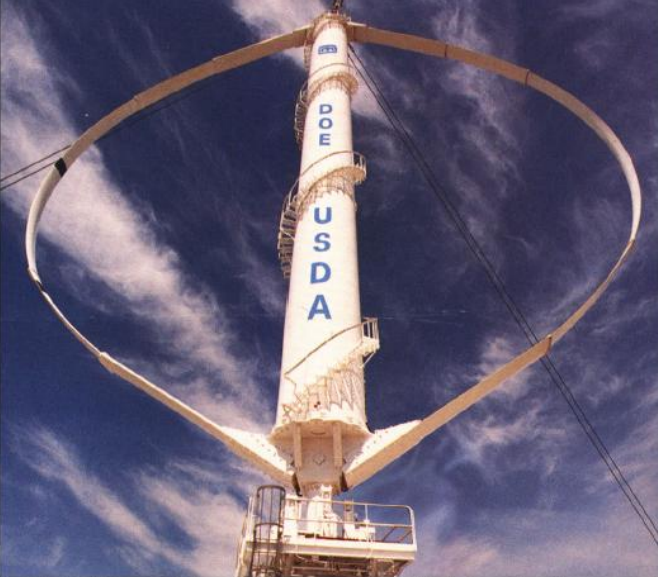
\includegraphics[width=\textwidth]{Murray2011-34m}
        
        \caption{Sandia 34 m Test Bed, from \cite{Murray2011}.}
        
        \label{fig:Sandia-34m}
    \end{subfigure}
    \hfill
    \begin{subfigure}[b]{0.355\textwidth}
        \centering
        
        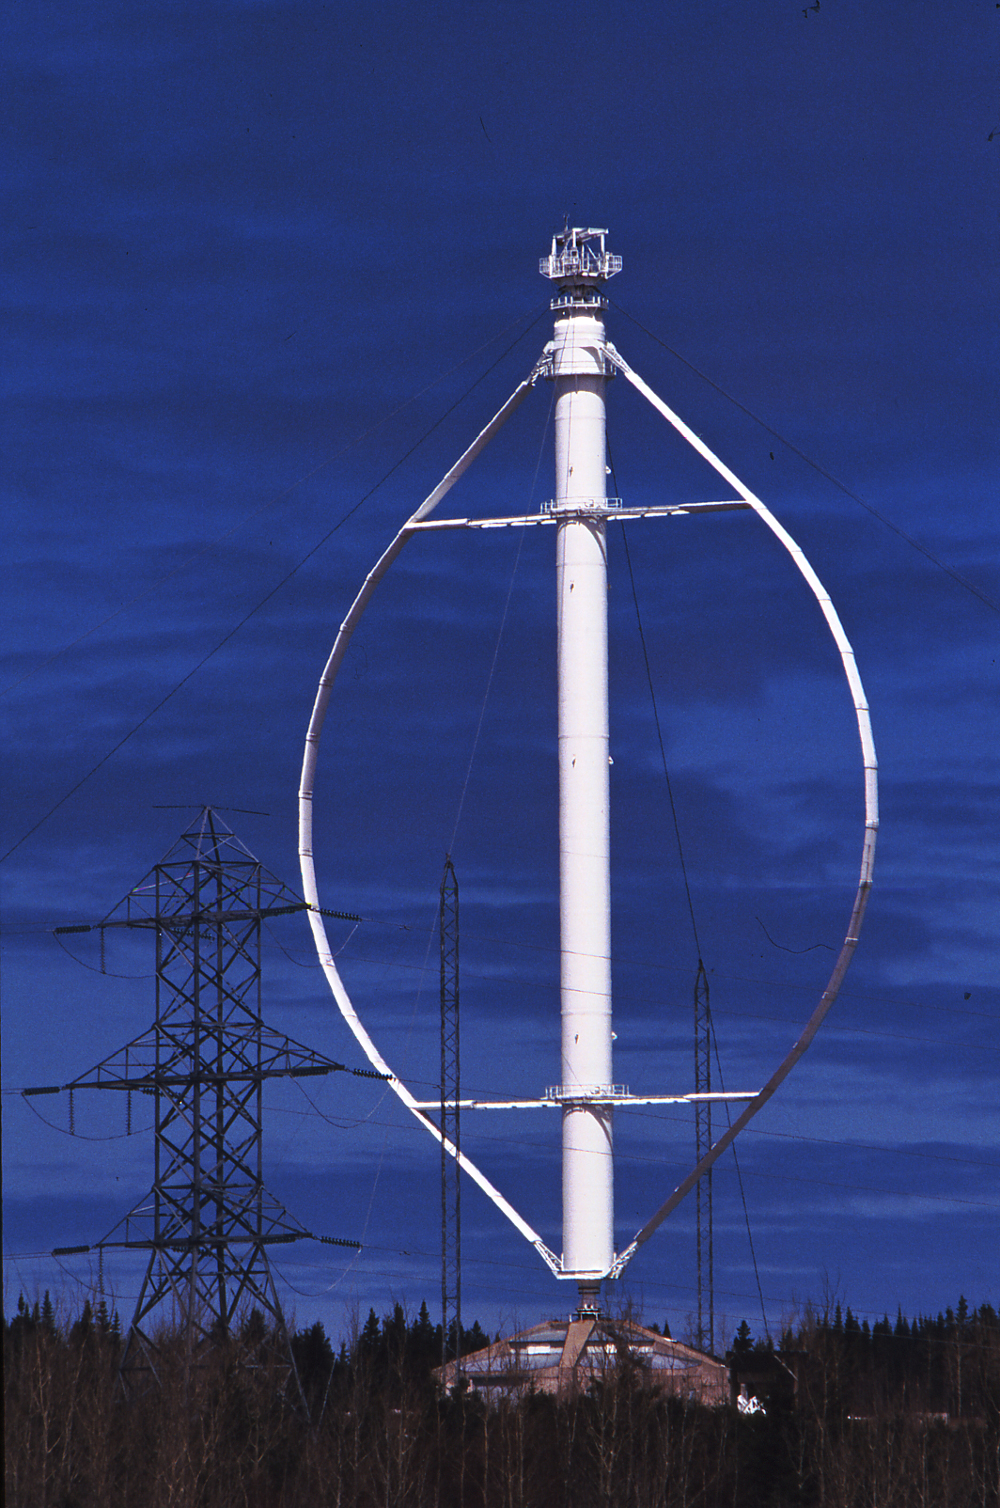
\includegraphics[clip, trim=0 0 0 0.05in, width=\textwidth]{Eole}
        
        \caption{Lavalin Eole 64 m VAWT. Photo by Paul Gipe. All rights
            reserved.}
        
        \label{fig:Eole}
    \end{subfigure}
    
    \begin{subfigure}[b]{0.8\textwidth}
        \centering
        
        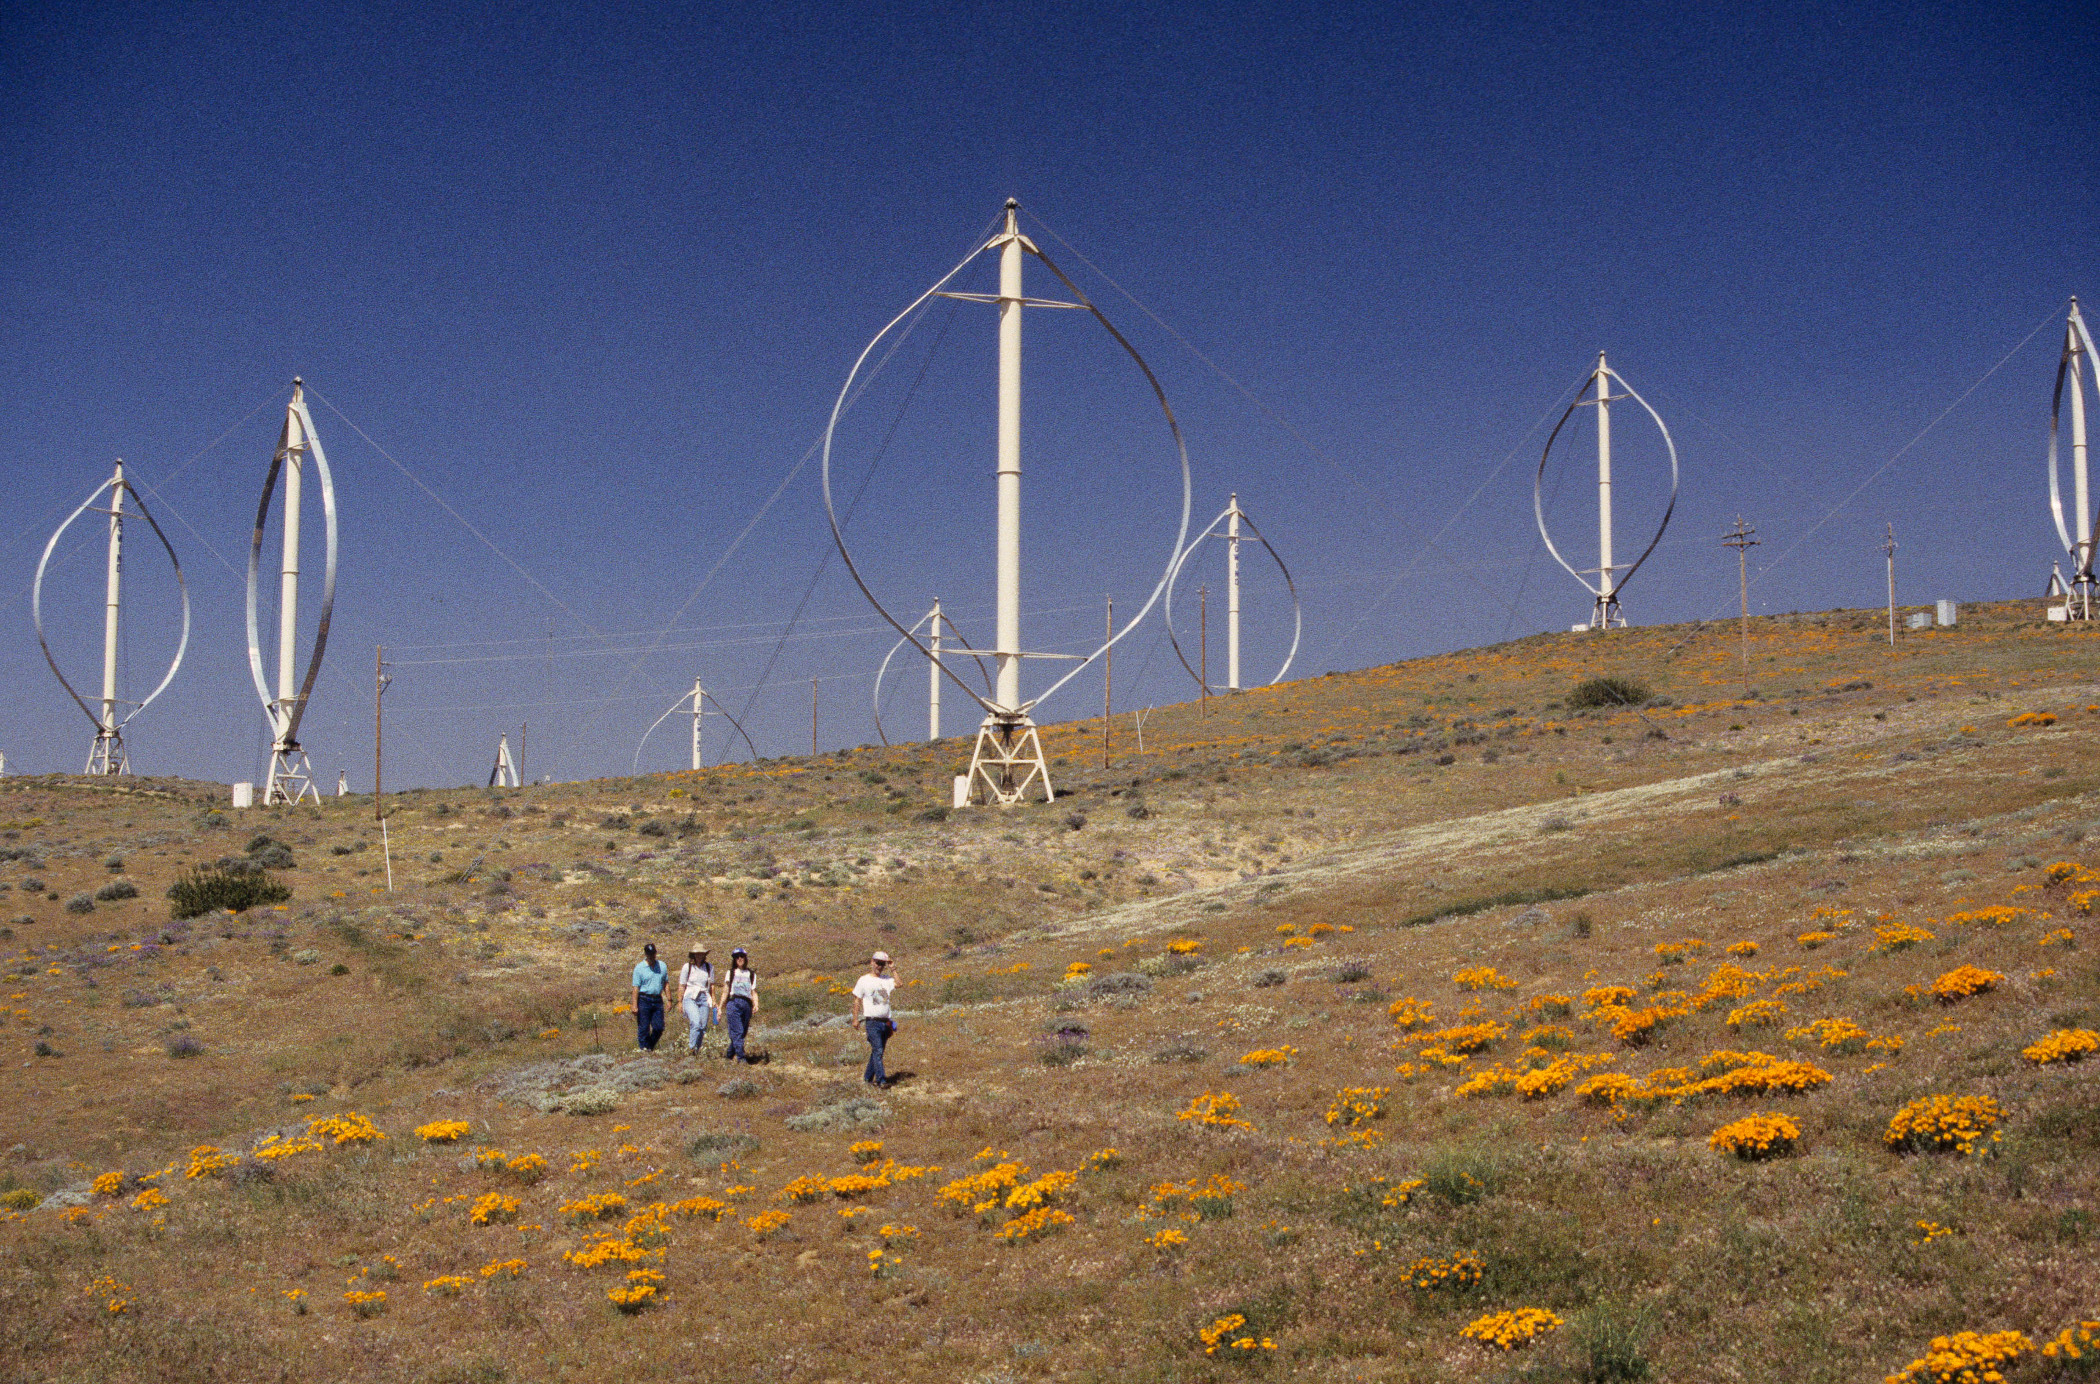
\includegraphics[width=\textwidth]{flowind}
        
        \caption{FloWind VAWT array. Photo by Paul Gipe. All rights reserved.}
        
        \label{fig:FloWind}
    \end{subfigure}
    
    \caption{Large scale Darrieus wind turbines: Sandia 34 m Test Bed (a),
        Lavalin Eole 64 m (b), and FloWind VAWT array (c).}
    
    \label{fig:Darrieus}
\end{figure}

Ultimately the three-bladed, horizontal-axis propeller-type axial-flow turbine
(AFT) concept---shown in Figure~\ref{fig:AFT} has became the design of choice
for large scale onshore wind---and for good reasons. Axial-flow turbines are
easier to analyze since their operating principles can be though of as an
essentially steady flow over a foil before stall. AFTs also have the benefit of
research ``inertia''---a lot has been invested and a lot of knowledge has
accumulated already. As a result, the designs are quite mature, for wind energy
at least. In contrast, the CFT has been studied and applied significantly less,
though there have been cases where CFTs have performed nearly equivalently well
as AFTs. However, CFTs are harder to design, since their blades are constantly
changing their angles of attack throughout the turbine's rotation, often
undergoing dynamic stall as part of normal operation \cite{Para2002}. Beside
their unpredictability, the highly oscillatory blade loading presents
significant design challenges for avoiding fatigue---a main cause for failure or
premature retirement of the large Darrieus wind turbines.

\begin{figure}[ht]
    \centering
    
    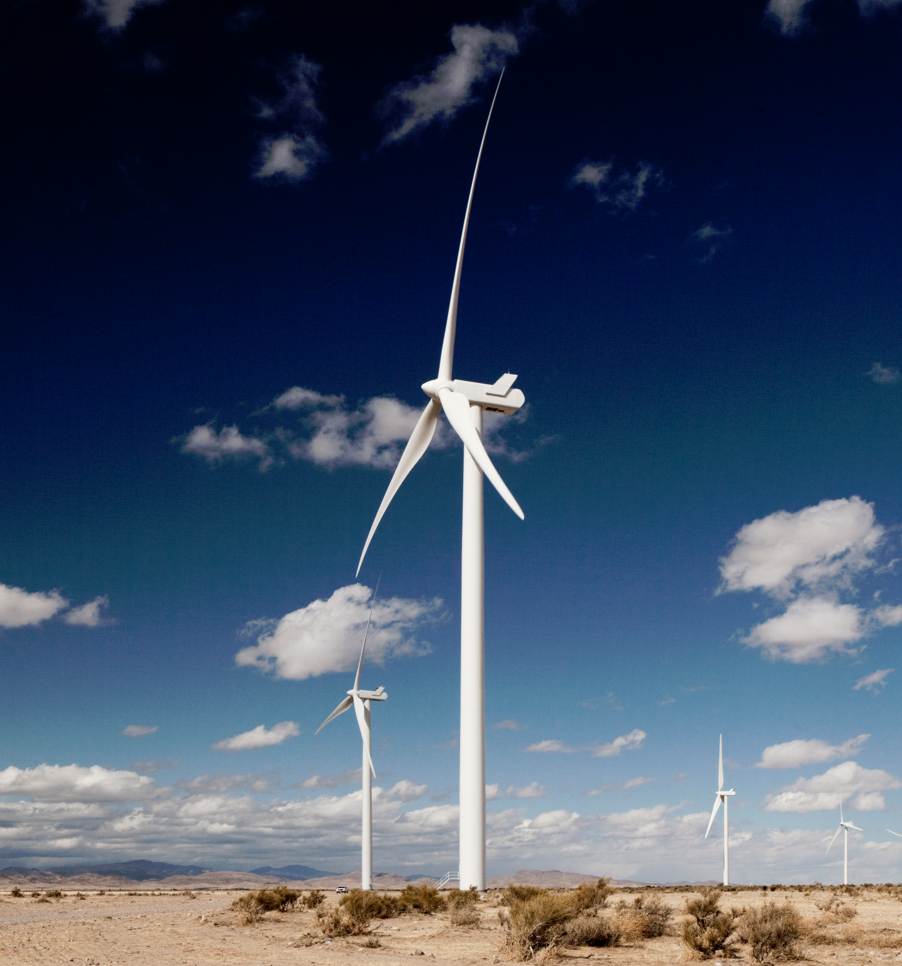
\includegraphics[width=0.7\textwidth]{Vestas-V100}
    
    \caption{Vestas V100 1.8 MW three-bladed axial-flow, a.k.a horizontal-axis
        wind turbine. Courtesy of Vestas Wind Systems A/S.}
    
    \label{fig:AFT}
\end{figure}

Despite their shortcomings, CFTs still may be valuable in some cases. They are
simpler, omni-directional machines, which negates the need for yawing and
pitching mechanisms. There were considerations in the 2010s by DEEPWIND in
Europe \cite{Paulsen2011} and SNL \cite{Sandia2012} in the US for using large
scale floating VAWTs for offshore wind, since along with the
omni-directionality, a vertical shaft allows placement of the generator and
gearbox lower in the machine, which lowers center of gravity. In the onshore
wind arena, CFTs show promise for projects where space is limited, e.g., urban
environments, as adjacent turbines sometimes interact ``constructively'' to
increase each other's power outputs \cite{Li2010}---a trait not possessed by
AFTs. A group from the California Institute of Technology has shown that arrays
of VAWTs can potentially provide an order-of-magnitude increase in the power
output per land area of a wind turbine array, since the devices can be spaced
more closely than HAWTs \cite{Dabiri2011}. Field measurements have shown that
their wakes recover more quickly than those of AFTs, and this cannot be entirely
attributed to higher turbulence generation \cite{Kinzel2012}. This phenomenon is
investigated in later chapters.

In the built, i.e., suburban and urban environments, wind resources are less
understood, more variable in terms of direction, speed, and turbulence levels
\cite{Smith2012}. Kooiman and Tullis \cite{Kooiman2010} observed that a
cross-flow turbine in an urban environment was indeed insensitive to changes in
wind direction, and was only adversely affected by temporal variations in wind
speed when turbulence intensity was above 15\%. The lack of need for yawing can
help lower cost of energy from CFTs versus AFTs by reducing complexity, e.g., by
eliminating slip rings. Cross-flow turbines may also have an advantage in the
urban environment since they must be designed for high fatigue loads anyway.
Recently, the Eiffel tower in Paris, France has been outfitted with two 5.3 m
tall, 3.2 m diameter helical vertical-axis cross-flow turbines, which will
produce at least 10 kWh/yr, or approximately 1 kW on average, which is expected
to power the entire first floor of the facility \cite{Lott2015}.

For MHK development, a field much less mature than wind power, the cross-flow
turbine concept is playing a major role thanks to its omni-directionality and
flexibility with respect to frontal area shape, allowing for more precisely
tuned fitment in channels with complex bathymetry or installed structures.
Chosen by the Ocean Renewable Power Company (ORPC) for their TidGen design, a
cross-flow turbine was the first grid-connected tidal energy device in the US,
which was installed in Cobscook Bay, ME \cite{ORPC2012}. Today, ORPC is working
on improving their turbine's performance, and planning for the installation of 4
more turbines \cite{Nelson2013}. 

CFTs are also being considered for micropower applications, such as powering
remote underwater instrumentation packages that currently rely on batteries
\cite{Polagye2013b}. They are also being used in riverine applications, for
example, in ORPC's RivGen project in the Kvichak River just downstream of the
village of Igiugig, AK~\cite{Forbush2015}, and the Rosa canal in Yakima, WA
\cite{Gunawan2014}. 

In general, the failure of cross-flow turbines in the large scale wind industry
can be largely attributed to less-than-adequate predictive capability in the
engineering process, i.e., issues with low performance and fatigue could be
overcome. In order for modern cross-flow turbines to be effective, these
capabilities must be enhanced, for both individual devices and arrays, which is
a primary motivation for this research.


\section{Principles of cross-flow turbine operation}

Blade element theory, originally conceived by
Drzewiecki~\cite{Drzewiecki1892,Drzewiecki1920}, is the analysis of a rotor or
propeller as a collection of 2-D foil sections, or blade elements, and can be
employed to obtain a simplified view of the kinematics and dynamics of a CFT.
Figure~\ref{fig:vectors} shows the relevant velocity and and force vectors on a
CFT blade element. The relative velocity and angle of attack $\alpha$ are
calculated by adding the inflow velocity vector to the opposite of the blade
element velocity $\omega R$, where $\omega$ is the shaft angular velocity and
$R$ is the element radius. In the relative velocity coordinate system, the lift
and drag are then oriented normal and tangential to the relative velocity,
respectively. These forces ultimately produce the shaft torque, and in turn the
shaft power.

\begin{figure}[ht]
    \centering
    
    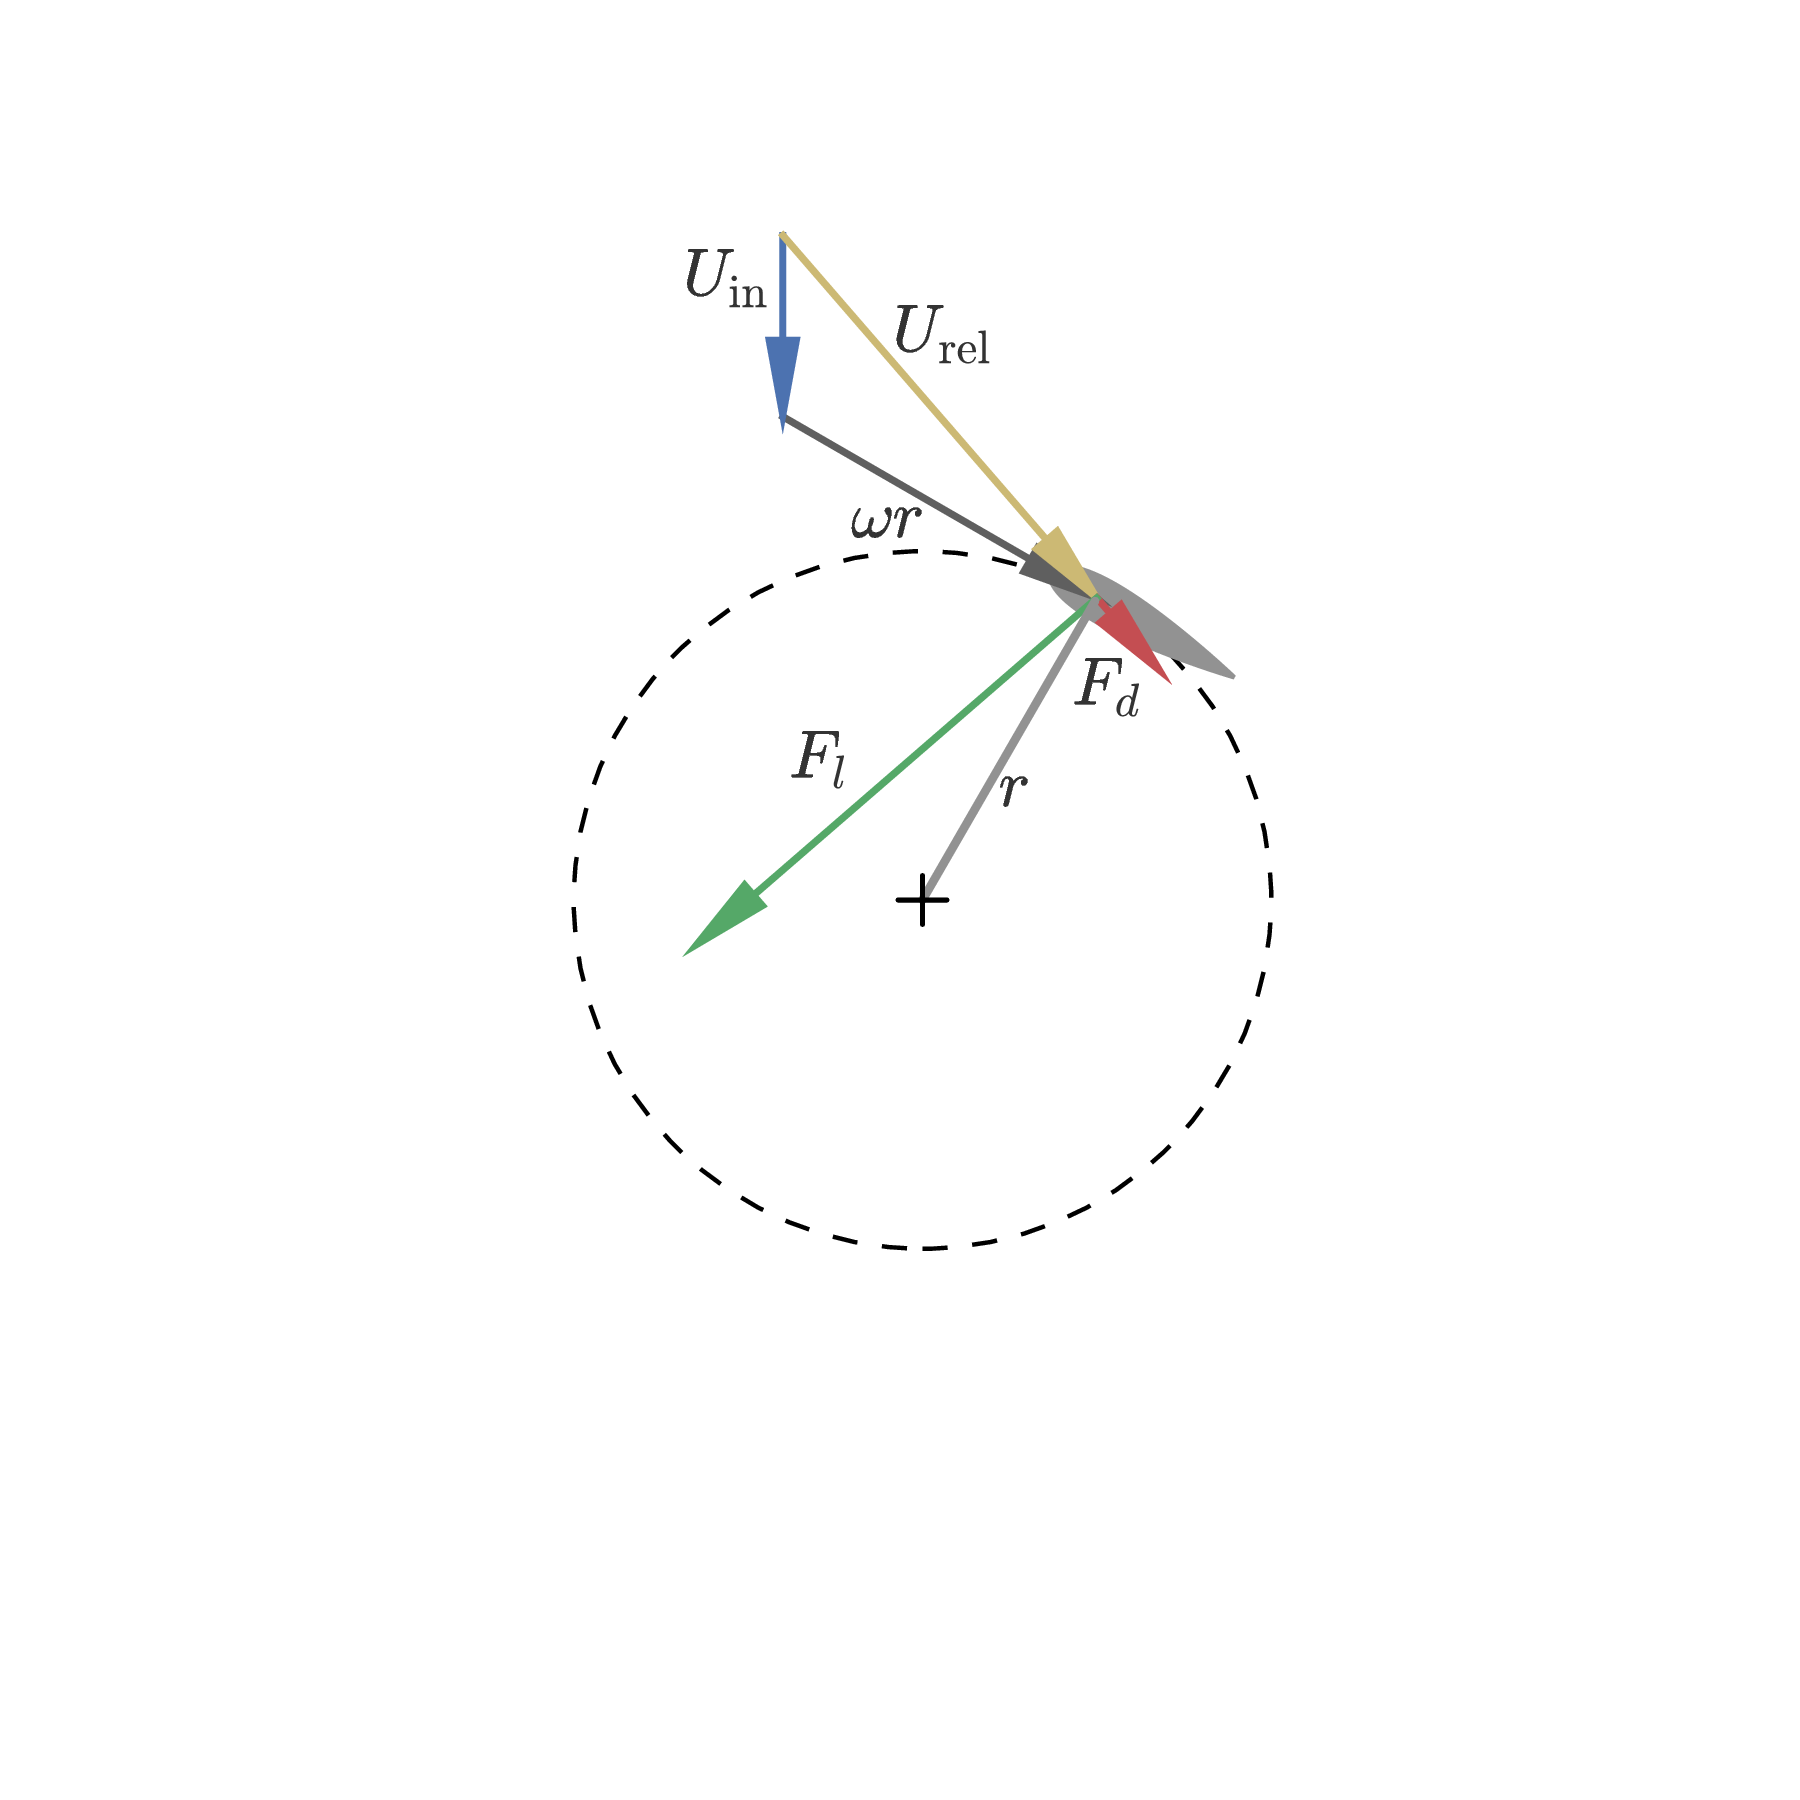
\includegraphics[clip, trim=1in 1.5in 1in 0.5in,
    width=0.6\textwidth]{figures/CFT-vectors_cft-vectors}
    
    \caption{Vector diagram of velocity and forcing on a cross-flow turbine
        blade element.}
    
    \label{fig:vectors}
\end{figure}

The shaft's angular velocity is nondimensionalized as the tip speed ratio
\begin{equation}
    \lambda = \frac{\omega R}{U_\infty},
    \label{eq:lambda}
\end{equation}
where $U_\infty$ is the free stream velocity.
Torque $T$ is characterized by the nondimensional torque coefficient 
\begin{equation}
    C_T = \frac{T}{\frac{1}{2} \rho A R U_\infty^2},
    \label{eq:ct}
\end{equation}
where $\rho$ is the fluid density and $A$ is the turbine's frontal area.
Similarly, the turbine power $P = T\omega$ and overall rotor drag $F_D$ are
normalized as the power coefficient
\begin{equation}
    C_P = \frac{T \omega}{\frac{1}{2} \rho A U_\infty^3},
    \label{eq:cp}
\end{equation}
and the rotor drag coefficient
\begin{equation}
    C_D = \frac{F_D}{\frac{1}{2} \rho A U_\infty^2}.
    \label{eq:cd}
\end{equation}
It is also worth noting that $C_P = \lambda C_T$.

So why then, is it difficult to analyze these machines? A first glimpse can be
seen in Figure~\ref{fig:geom-alpha-urel}, where the geometric angle of attack
and relative velocity are plotted over one turbine revolution for various tip
speed ratios. If we imagine a typical high solidity $\sigma = Nc/R$ turbine
operating at an optimal tip speed ratio $\lambda_0 = 2$, for example
\cite{Howell2010} (note that solidity and $\lambda_0$ are inversely correlated
\cite{Templin1974}), we see that angles of attack can be very high even in
optimal conditions. Keep in mind that we are calculating geometric angle of
attack---the ``true'' angle of attack will be reduced by a slowing of the inflow
velocity, also known as induction.

\begin{figure}[ht]
    \centering
    
    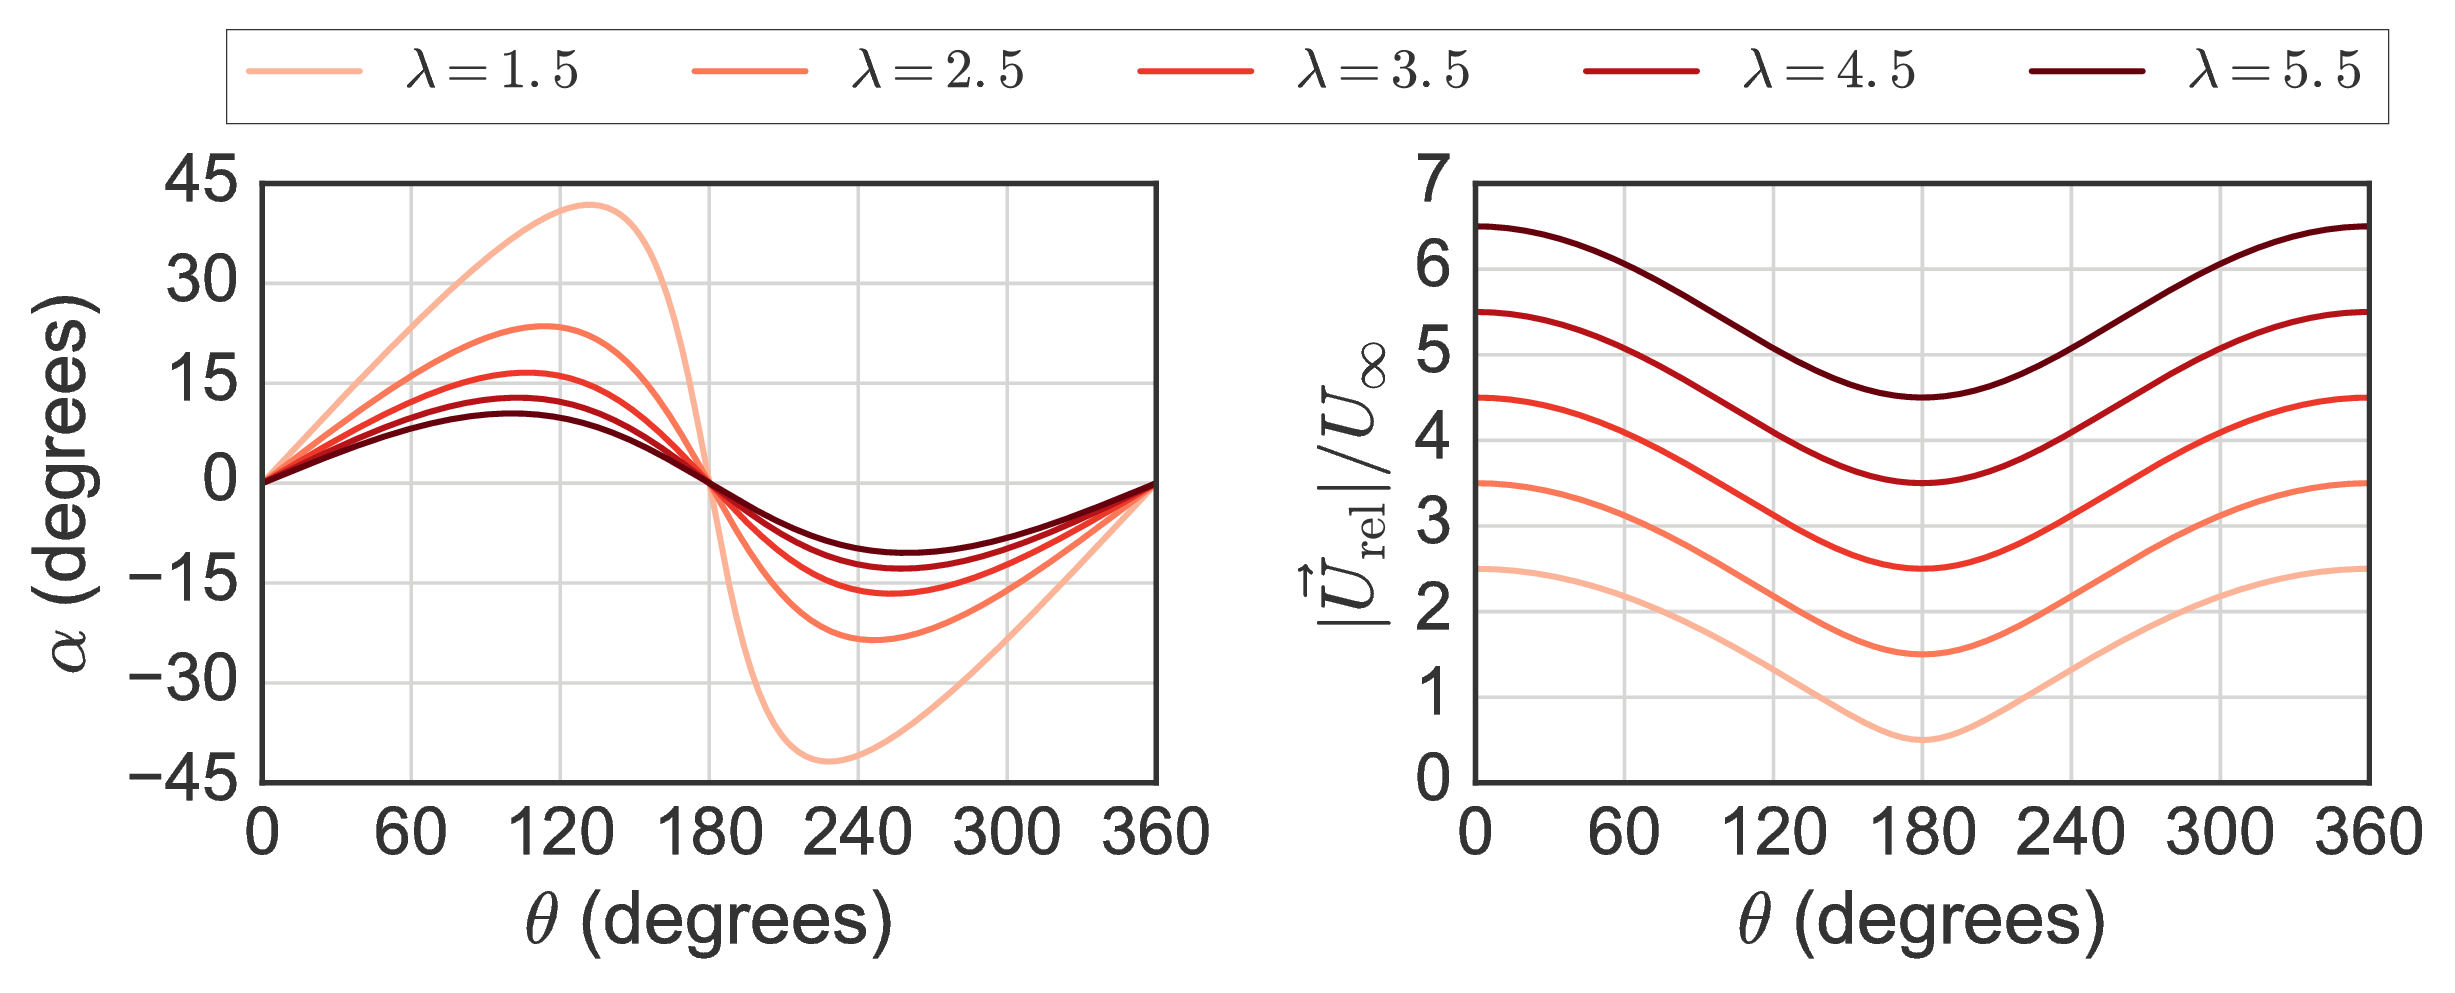
\includegraphics[width=0.85\textwidth]{CFT-vectors_alpha_deg_urel_geom}
    
    \caption{Geometric angle of attack (left) and relative velocity (right)
        versus azimuthal angle at various tip speed ratios.}
    
    \label{fig:geom-alpha-urel}
\end{figure}

As shown in Figure~\ref{fig:vectors}, the blade's lift to drag ratio and angle
of attack can be thought of as the quantities to maximize in order to develop
shaft torque. However, beyond a threshold angle of attack, i.e., the static
stall angle, $C_l/C_d$ drops. Predicting foil characteristics (lift, drag,
pitching moment) is difficult beyond the static stall angle, where boundary
layer separation becomes dominant over most of the foil suction surface, which
reduces lift and increases drag dramatically. For example,
Figure~\ref{fig:S826-perf} shows measured lift and drag coefficients compared
with 2-D and 3-D Navier--Stokes CFD simulations from Cakmakcioglu \etal
\cite{Cakmakcioglu2014}. The linear lift slope region and static stall angle are
predicted well enough, but the peak $C_l/C_d$ is massively overestimated. This
may not be an issue for a machine designed to operate at relatively fixed and/or
pre-stall $\alpha$, e.g., airplane wings, propellers, or axial-flow wind
turbines, but a cross-flow turbine will most likely encounter post-stall
regimes, making even high-fidelity CFD analysis an uncertain prospect for
accurate blade load prediction.

\begin{figure}[ht]
    \centering
    
    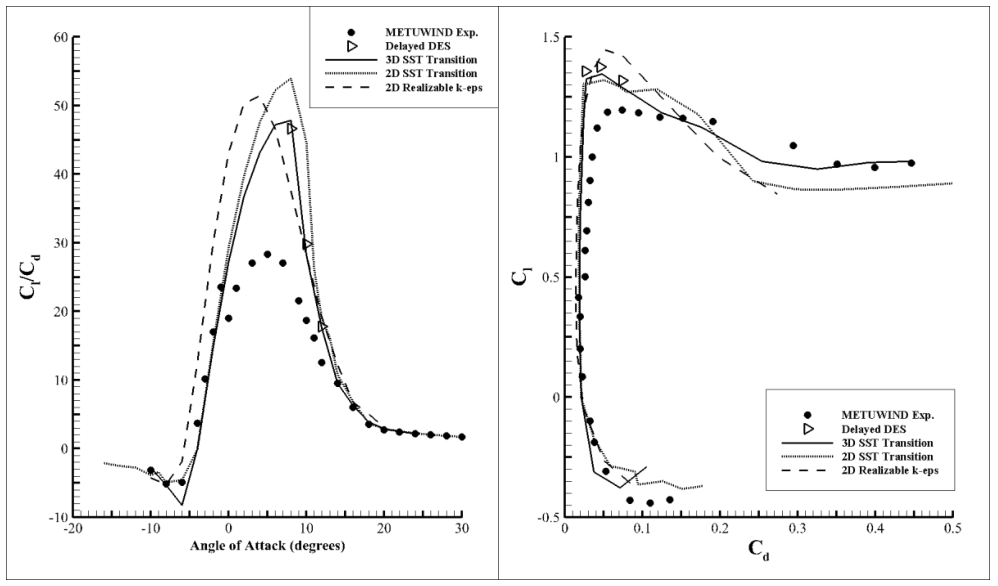
\includegraphics[width=\textwidth]{Cakmak-et-al-2014-fig8}
    
    \caption{Characteristics of an S826 airfoil at $Re=145,000$, from
        \cite{Cakmakcioglu2014}.}
    
    \label{fig:S826-perf}
\end{figure}


\subsection{Unsteady aerodynamics and dynamic stall}

Up until now we have only considered the static behavior of foils, which may be
sufficient to model the steady performance of an axial-flow turbine, since rotor
blade element angles of attack are meant to remain constant in ideal conditions.
The rotation of a cross-flow turbine, however---with its constantly changing
angle of attack (also the change in sign) and relative velocity---produces an
unsteady environment for the blade elements, even in an idealized case.

Unsteady foil behavior had been studied extensively in rotorcraft research. In
the absence of stall, even a helicopter rotor airfoil will deviate from static
behavior due to cyclic pitching, along with changes in relative velocity as the
blade advances and retreats. Thus, the wealth of knowledge available from the
helicopter literature provides insight into the cross-flow turbine case.

The first consideration is the attached behavior of unsteady airfoils. As one
might expect, in these cases either the angle of attack or relative velocity is
varying, but large amounts of flow separation, i.e. stall, is never encountered.
The unsteadiness is characterized by a reduced frequency~\cite{Leishman2006}
\begin{equation}
    k = \frac{\omega c}{2 U_\infty},
\end{equation}
which assumes the free stream velocity is constant. Unsteady effects begin to
become significant for $k > 0.05$, and can become dominant for $k \ge 0.2$.

For a cross-flow turbine reduced frequency can be reformulated in terms of the
tip speed ratio as
\begin{equation}
    k = \frac{\lambda c}{2R}.
\end{equation}
As an example, a large scale, relatively low solidity Darrieus turbine such as
the Sandia 34 m diameter Test Bed, with an equatorial blade chord of 0.91 m
\cite{Murray2011}, a reduced frequency of 0.16 is encountered based solely on
angle of attack oscillations at $\lambda=6$. For a smaller scale CFT, e.g., with
$c/R = 0.25$, operating at $\lambda = 2$, the reduced frequency is 0.25. It
follows that unsteady effects will be significant for cross-flow turbines even
in the absence of nonlinear effects such as stall.

In the unsteady regime, when angle of attack is high enough to induce large
separation it is called dynamic stall. The effects on foil loading are different
from those of static stall in that they are time dependent and include
hysteresis or lag effects. The dynamic stall process in general can be described
as \cite{McCroskey1981}:
\begin{enumerate}
    \item A large leading edge vortex is formed, which causes an overshoot in
    lift beyond the static case in a linear fashion.
    
    \item The vortex is advected downstream, causing additional lift.
    
    \item The vortex reaches the trailing edge and the lift decays rapidly.
    
    \item Lift slowly returns to the linear regime as flow reattaches.
\end{enumerate}

Based on Figure~\ref{fig:geom-alpha-urel}, we expect dynamic stall to play an
important role in governing overall blade loading for a cross-flow turbine.
Therefore, it is necessary to either accurately model dynamic stall, or employ
CFD methods that can resolve unsteady effects in the foil boundary layer, both
of which will be explored in later chapters.


\section{The state of engineering tools for CFTs}

\subsection{For individual devices}

Presently, the most reliable predictor of turbine performance is physical
modeling (building prototypes or copying existing designs that have been
field-tested), so long as important dynamical scales (Reynolds number, mainly)
are sufficiently matched. It has been shown that performance becomes essentially
Reynolds number independent at an approximate blade chord Reynolds number $Re_c
\approx \lambda U_\infty c / \nu = O(10^5)$ \cite{Bravo2007}, which is
investigated further in later chapters. However, experiments at this scale can
be quite expensive. For example, a turbine with a 1 m diameter and 10 cm chord
would need to be tested in a flow on the order of 1 m/s in water and 10 m/s in
air. For a turbine this large it is typically impractical to manufacture many
prototypes to find the optimal design, so numerical modeling is preferred. There
exists a large spectrum of numerical modeling techniques with widely varying
computational cost and fidelity, and sometimes only the most complex and
computationally expensive are trustworthy.

Momentum models are the simplest and cheapest, where the turbine blades are
discretized into blade elements, for which 2-D static lift and drag data are
tabulated. The relative velocity and angle of attack for a blade element are
calculated by seeking a balance between forces computed from the static foil
data and the rate of change of momentum of the fluid passing by the blade
element. Momentum methods break down for large streamwise forces, i.e.,
``induction factors''---common in water and high solidity turbines---and must be
corrected empirically. Despite their deficiencies, these models can do a
reasonable job for low solidity rotors when combined with corrections for
dynamic loading, the most prominent cause of which is dynamic stall
\cite{Para2002}, but fail for high solidity~\cite{Joo2015}. A double multiple
streamtube (DMS) momentum model can compute a full turbine performance curve in
seconds on a modern desktop computer.

Vortex line methods are similar to momentum models, except blade element local
velocity is computed using potential flow theory, where lifting bodies are bound
vortex lines that shed vortex wake elements whose influences are combined via
the Biot--Savart law \cite{Strickland1979}. Sandia National Labs' CACTUS is an
example of a vortex method \cite{Murray2011}. CACTUS has been tested against
experimental data from large, low-solidity wind turbines (those for which
momentum models do well), but has been shown to fail for smaller turbines in
water, which are typically higher solidity \cite{Michelen2014}. Regarding
computing effort, vortex line methods can compute a full turbine performance
curve in minutes---slightly longer than the DMS method, but still quite fast.
The increase in accuracy of the flow field prediction and the robustness with
respect to high turbine loading justify the slightly higher expense of the
vortex line method.

A more sophisticated vortex model is the so-called panel method, where turbine
geometry can be specified arbitrarily as potential flow boundary elements,
negating the need for sectional foil coefficient tables. This is a significantly
more computationally expensive model. A single turbine operating point (not a
full performance curve) computed in three dimensions may take hours on a
conventional desktop PC. Furthermore, boundary layer models are necessary to
predict the occurrence and consequences of dynamic stall \cite{Zanon2012}.

The most computationally expensive models solve the Navier--Stokes equations,
with turbulence modeled with Reynolds-averaging (RANS) or large eddy simulation
(LES)---the former being relatively less expensive, since LES directly solves a
larger portion of the energy spectrum of turbulence. If a body-fitted grid is
used, the actual turbine geometry is included as part of the computational
domain, and the mesh is generally refined next to the solid surfaces to resolve
the boundary layer, i.e., with cells adjacent to walls having a nondimensional
wall distance $y^+ \sim 1$. When only run in two dimensions, RANS methods are
affordable enough to be run on a single CPU, computing a single turbine
operating point in hours. However, 3-D effects are important enough that 2-D
simulations are not reliable, at least as predictors of absolute performance
\cite{Li2013}. 3-D simulations with a body-fitted grid are very expensive
(especially for LES), therefore are practically limited to high performance
computing (HPC) clusters. Even with the high computational expense, these models
are not perfect and results can deviate significantly from experimental
measurements, especially when using RANS models \cite{Li2013}.

Actuator line modeling (ALMs), first used by Sorensen and
Shen~\cite{Sorensen2002}, is a hybrid of the blade element and Navier--Stokes
methods. The turbine is not part of the mesh, but is represented by lines that
move through the flow, acting as momentum sinks, where the resultant force is
computed using 2-D foil data. Negating the needs for a body-fitted grid and
resolving the boundary layer removes a significant amount of computational
effort, but the flow field is still computed more accurately than with momentum
or vortex methods, since nonlinear effects and turbulence are included in the
RANS or LES equations. Removing the need for complex grids is also an advantage
with respect to  mesh generation, which is arguably the largest impediment to
automation in CFD \cite{Slotnick2014}. Computational effort is also
significantly reduced since the ALM does not need a rotating mesh.

To the author's knowledge, at the time of
this writing there has only been one study in the literature investigating the
ALM for CFTs \cite{Shamsoddin2014}, which was performed for a 2-D rotor at very
low Reynolds number, for which performance predictions were not reported.
Assessing its effectiveness is therefore of interest in the present work.


\subsection{For arrays}

Effective turbine array engineering directly depends on accurate prediction of
turbine wake generation, evolution and interaction, along with the impact of
various types of turbulent inflow on power production of each device. Like for
individual turbines, physical modeling is an option for predicting array
performance, though it becomes even more expensive to match relevant dynamical
scales. For this reason, turbine arrays are mainly designed using numerical
methods.

The contemporary industry standard method for predicting array performance
involves the superposition of prescribed wakes \cite{Stevens2014b}. Evolution
can be dependent on a single expansion coefficient chosen by the free stream
turbulence intensity \cite{Jensen1983, Choi2013} or computed by a solution of
the linearized RANS equations with an empirically derived constant eddy
viscosity closure \cite{Ainslie1988}. In light of the CFT's unique near-wake
dynamics, the valitidy of these models is questionable. At the very least they
would need to be recalibrated for CFTs, though their applicability is limited in
the near-wake of any turbine, meaning they are generally inappropriate for
closely-spaced arrays.
	
The next step up in complexity is the actuator disk method, where a constant
body force is added to the Navier--Stokes equations. This method can be
computationally cheap with RANS, or quite expensive and thorough with LES. The
ORPC turbine array is being laid out using the SNL-EFDC code, which uses a
constant uniform force applied to the RANS equations, where the turbine injects
turbulence kinetic energy and dissipation for the model's $k$--$\epsilon$
closure \cite{Nelson2013}. The ability of actuator disk models to predict the
near-wakes of CFTs is of interest in this work.
	
At present simulations with body-fitted grids are limited to one or two turbines
due to computational cost, which means they are impractical for full array
simulations. Thus the actuator line method, when combined with LES, is the most
complex model being used today. The ALM has the benefit of resolving unsteady
flow features created by periodic blade forcing and end effects, ultimately
producing the most accurate parameterization for turbine induced forces in
Navier--Stokes simulations. It has been shown in blind axial-flow turbine
modeling tests that ALM/LES methods fair better when predicting turbine induced
turbulence, and therefore will be more accurate at predicting flow within a
turbine array \cite{Krogstad2013}.


\section{Goals and objectives}

At the most basic level, the goal this research is to work towards the ability
to predict the performance of and flow though an array of cross-flow turbines,
to allow for the evaluation of array layouts, and the prediction of overall
power output and potential environmental effects. The strategy for meeting this
goal includes the following objectives:

\begin{enumerate}
	\item To improve the understanding of both high and low solidity cross-flow
    turbine wakes, most importantly the apparent increased rate of recovery
    compared with axial-flow turbines. This will establish our flow modeling
    targets.
    
    \begin{enumerate}
        \item To evaluate the ability of actuator disk models to predict the
        wakes of cross-flow turbines.
    \end{enumerate}
	
	\item To assess the allowable scale mismatch at which physical models can
	provide results relevant to full-scale devices and arrays.
	
	\item To evaluate the ability of high-fidelity blade-resolved computational
    fluid dynamics and high performance computing to supplement or possibly replace
    experimental work.
    
    \item To investigate actuator line modeling to potentially reduce the
    required computing power necessary for engineering work with CFTs.
\end{enumerate}


\section{Contributions to science and engineering}

Cross-flow turbines are simple machines made from common shapes, but they can
produce very complex flows. Despite their failure in the large scale wind
industry, and beyond their contemporary adoption in marine hydrokinetics, there
is scientific and engineering value to better understanding their behavior. The
flow problem---unsteady foil behavior involving dynamic stall, finite blade span
end effects in curvilinear flows---is complex yet general enough to be
applicable to other unsteady turbomachinery and/or foil flows, e.g., Voith
Schneider propellers, Cyclogyros, or even conventional helicopter rotors.

This work will increase the amount of experimental data available for device
comparison and numerical model validation. This is especially important for CFTs
since typical designs for small wind and MHK use have not yet been established.
This means that in order to be robust, numerical models must be tested against
measurements from turbines with varying design parameters, notably the solidity
and aspect ratio, which affect the unsteadiness and significance of 3-D effects,
respectively. There is a danger that validating against the most ubiquitous
Darrieus turbine experiments may result in models that fail with newer, more
unique designs.

From this work, open datasets have been generated and published. These datasets
will help others evaluate their numerical models, and since their availability
will also include processing code, other researchers may find new knowledge to
glean from them. 

In summary, this research will elucidate the unique wake properties of
cross-flow turbines, establish scaling guidelines for physical modeling, and
inform designers on the trustworthiness of state-of-the-art numerical modeling
techniques.

% Chapter on developing experimental setup
\chapter{Development of an experimental setup for measuring the performance and
    near-wake of cross-flow turbines at large laboratory
    scale}\label{chap:exp-setup}

In 2011, a turbine test bed was developed for measuring the performance
(mechanical power and overall rotor drag or thrust) of large laboratory scale
($O(1)$ m\textsuperscript{2} frontal area) cross-flow turbines in the University
of New Hampshire (UNH) tow tank \cite{Bachant2011-MS}, a 36.6 m long, 3.66 m
wide, and 2.44 m deep facility, pictured in Figure~\ref{fig:tow-tank}, which was
capable of towing up to approximately 1.4 m/s. The turbine-specific
instrumentation consisted of a mounting frame built from NACA 0020 hydrofoil
struts, a hydraulic disk brake for turbine loading, an Interface T8 200 Nm
capacity rotary torque transducer, and a 54 pulse-per-rev magnetic pickup for
measuring shaft speed. The frame was mounted to the carriage via
streamwise-oriented linear bearings and was held in place by a pair of Sentran
ZB3 2224 N capacity load cells that allowed measurement of total streamwise
rotor drag.

\begin{figure}
    \centering

    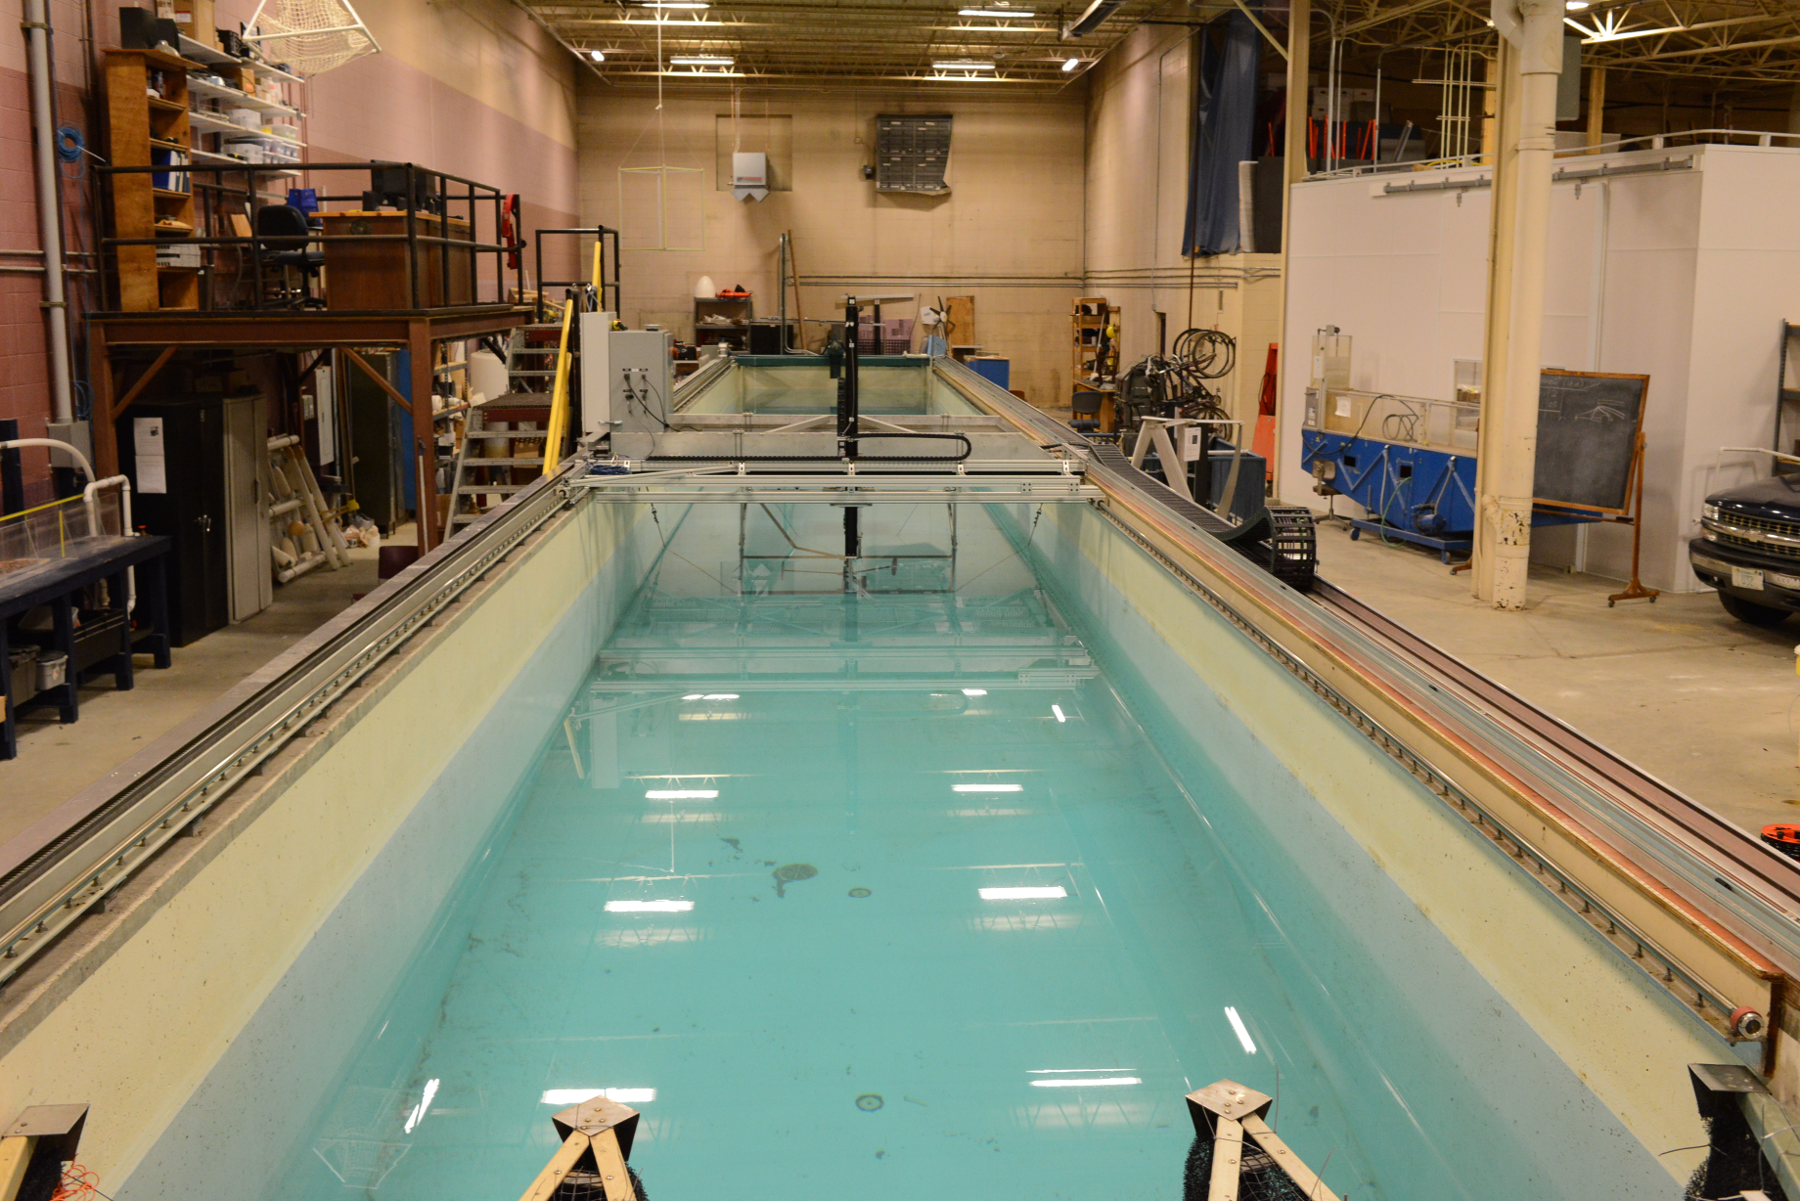
\includegraphics[width=0.9\textwidth]{tow-tank.png}

    \caption{The University of New Hampshire's wave and tow tank, located in the
        Jere A. Chase Ocean Engineering Laboratory.}

    \label{fig:tow-tank}
\end{figure}

Despite its usefulness in collecting a relatively small amount of data for two
helical cross-flow turbines~\cite{Bachant2015-RE}, this ``first generation''
system had some issues to be addressed:
\begin{itemize}
    \item No control over turbine shaft angular velocity. This made operation at
    tip speed ratio below peak torque impossible.

    \item Fully manual starting and load application. This limited resolution of
    the applied torque, and took considerable effort to perform experiments on
    the order of 100 tows, since a person had to ride on the tow carriage to
    adjust and apply the load torque.

    \item Open loop speed and manual position control of the tow carriage. This
    also took considerable effort to operate experiments, since the operator had
    to estimate braking distance to ensure the carriage did not hit the tank
    ends.

    \item Low carriage acceleration. The carriage acceleration was on the order
    of 0.1 m/s\textsuperscript{2}, which limited the steady state turbine
    operating duration to a few seconds.

    \item Low frequency resonance in the tow member. A long 0.25 inch diameter
    wire rope was used to tow the carriage, which resonated longitudinally with
    the significant variation of streamwise forces from the turbine.
\end{itemize}

In addition to the above issues, in order to meet the data acquisition goals, it
was necessary to measure turbine wake flows. These concerns required major
renovations, upgrades, and additions to the tow tank and turbine test bed
motion, control, and data acquisition systems. Furthermore, it was desirable to
automate the entire system to increase both data quality and quantity. These
changes were made possible thanks to an infrastructure grant from the US
Department of Energy (DOE).


\section{Modifications to the UNH tow tank}

The ``foundation'' of the experimental setup was the tow tank, which was
addressed first. The main goals for the tow tank upgrades were to increase max
speed and acceleration, add closed-loop positioning and velocity control,
stiffen the tow member to reduce longitudinal resonance, and add onboard power
and networking to the carriage for data acquisition and other peripherals. A
summary of the old system and new target specifications is shown in
Table~\ref{tab:tow-tank-specs}.

\begin{table}
\centering
\begin{tabular}{c|c|c}
Spec & Old system & Target \\
\hline
Maximum speed & 1.4 m/s  & 3.0 m/s \\
Maximum acceleration & 0.1 m/s$^2$ & 2.0 m/s$^2$ \\
Control system & Open loop velocity only & Closed loop position/velocity \\
Onboard power & $4\times12$ V batteries & Continuous 120 and 220 VAC \\
\end{tabular}
\caption{Specifications summary for existing and upgraded tow tank systems.}
\label{tab:tow-tank-specs}
\end{table}


\subsection{Linear guides}

The previous linear guide system, shown in Figure~\ref{fig:old-linear-guides},
consisted of a ``master'' guide constructed from $4 \times 4$ inch fiberglass
tubing, and a ``slave'' guide constructed from aluminum angle, on which plastic
wheels rode. Over time, the fiberglass tubing had failed structurally and was
covered with stainless steel bars fixed with double-sided tape. These bars
shifted around considerably during towing and were a source of noise in the
measurements.

A new set of linear guides was designed from 1.25 inch diameter Thomson 440C
stainless steel linear shafts and super self-aligning linear bearings, shown in
Figure~\ref{fig:new-linear-guides}. The existing carriage was modified to
retrofit the linear bearings, and a series of parts were designed to adapt the
stainless shafts to the existing quasi-level mounting surfaces, which helped
keep cost down. The shafts were mounted via 3/8-24 inch threaded rods in
oversized holes to allow adjustment in all three dimensions, a concept which was
inspired by similar linear guide setups at the University of Minnesota's Saint
Anthony Falls Laboratory (SAFL). The shafts were aligned in the cross-tank
direction using a piece of monofilament line stretched along the path. The
vertical alignment was set by spacing the shaft from its mounting surface
equally along the path via machined blocks. When the existing level surfaces
were set in 1996, these were measured to be level within $\pm 1/16$
inches~\cite{Darnell1996}.

\begin{figure}
    \centering

    \begin{subfigure}{0.47\textwidth}
        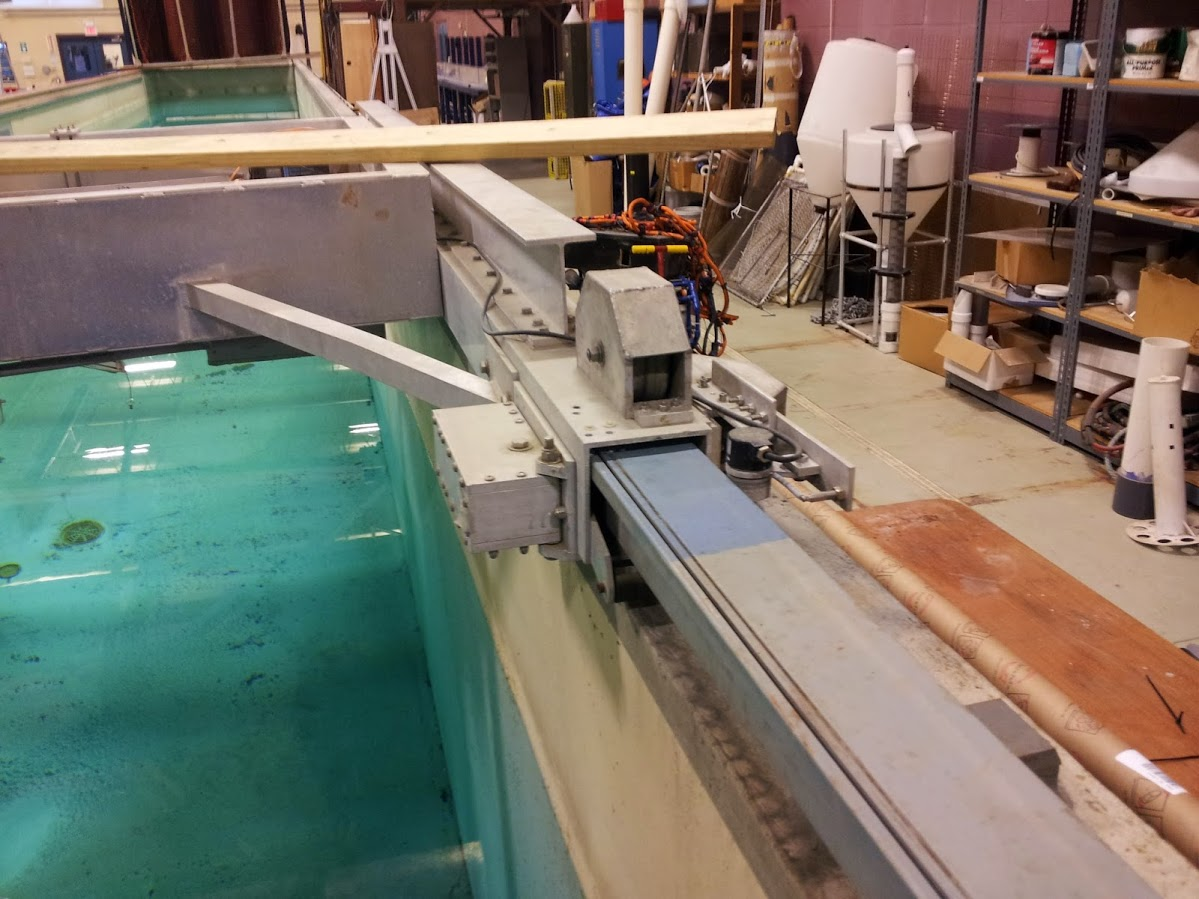
\includegraphics[width=\textwidth]{old-tow-tank-linear-guides}
        \caption{Previous linear guide system.}
        \label{fig:old-linear-guides}
    \end{subfigure}
    \begin{subfigure}{0.47\textwidth}
        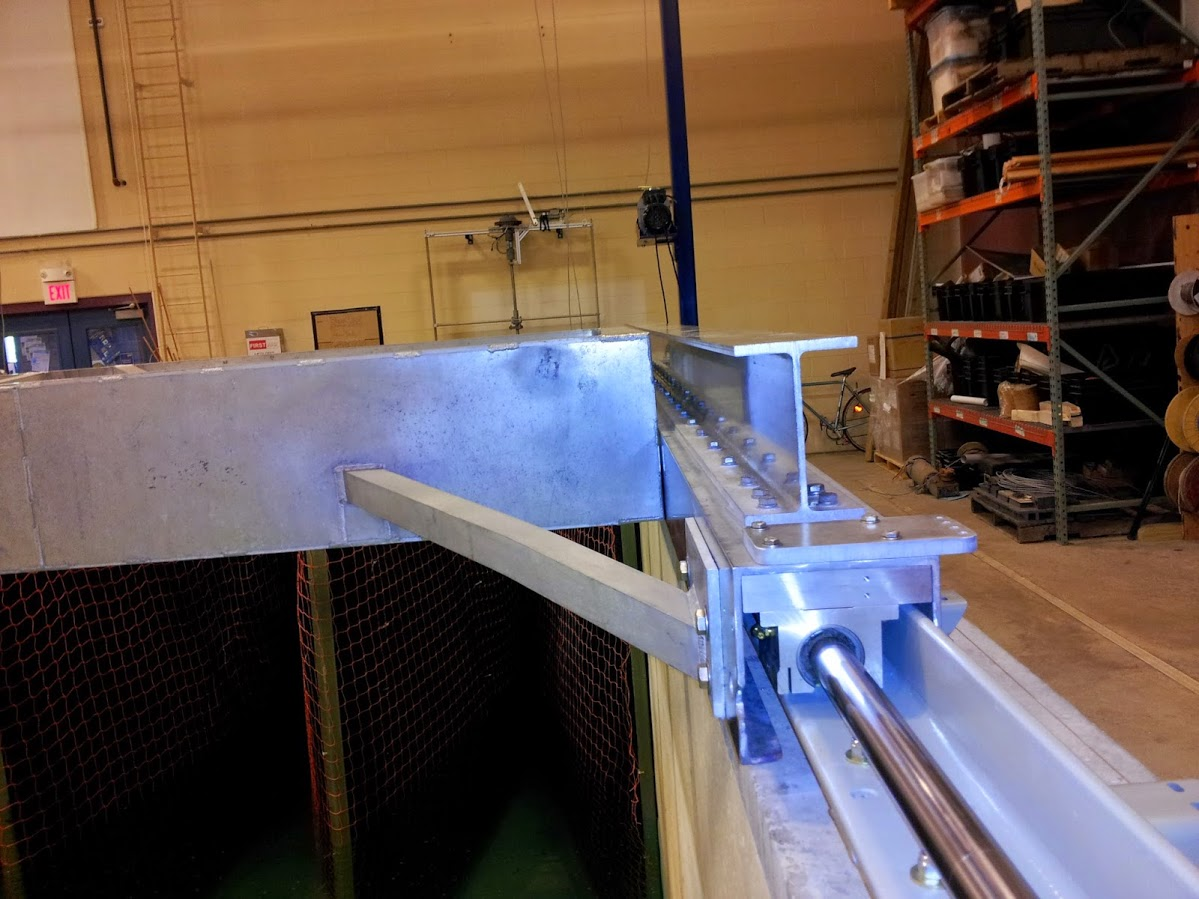
\includegraphics[width=\textwidth]{new-tow-tank-linear-guides}
        \caption{Upgraded linear guides.}
        \label{fig:new-linear-guides}
    \end{subfigure}

    \caption{Linear guide system (on ``master'' side) (a) before and (b) after
        upgrades.}
\end{figure}


\subsection{Motion and control}

The tow tank's previous motion system consisted of a 10 horsepower AC induction
motor powered by a Yaskawa V7 variable frequency drive. The motor was coupled to
a speed reducing gearbox, on which a pulley was mounted to drive a 0.25 inch
diameter wire rope. It was seen in previous testing that this system had very
low acceleration ($\sim 0.1$ m/s$^2$), which severely reduced steady state
towing durations. The relatively low spring constant of the wire rope tow member
also gave the system a low natural frequency, which resonated due to cross-flow
turbines' cyclic forcing. Furthermore, the system was only velocity-controlled,
and in an open-loop manner. This meant positioning was done manually, which took
a skilled operator, and reduced usable tank length further to allow for coasting
to a stop.

These issues were addressed by changing the motor to a 26.1 maximum horsepower
Kollmorgen AKM82 permanent magnet servo motor and 10:1 gearbox, shown installed
in Figure~\ref{fig:tow-servo}, which was sized to tow turbines with 1 m$^2$
frontal area up to 3 m/s, while accelerating at 2 m/s$^2$. The motor was powered
by a Kollmorgen S700 servo drive, controlled by an 8-axis ACS NTM EtherCAT
master controller, providing closed loop position and velocity control. A series
of emergency stop buttons were also installed to increase the safety of the
system.

\begin{figure}
    \centering

    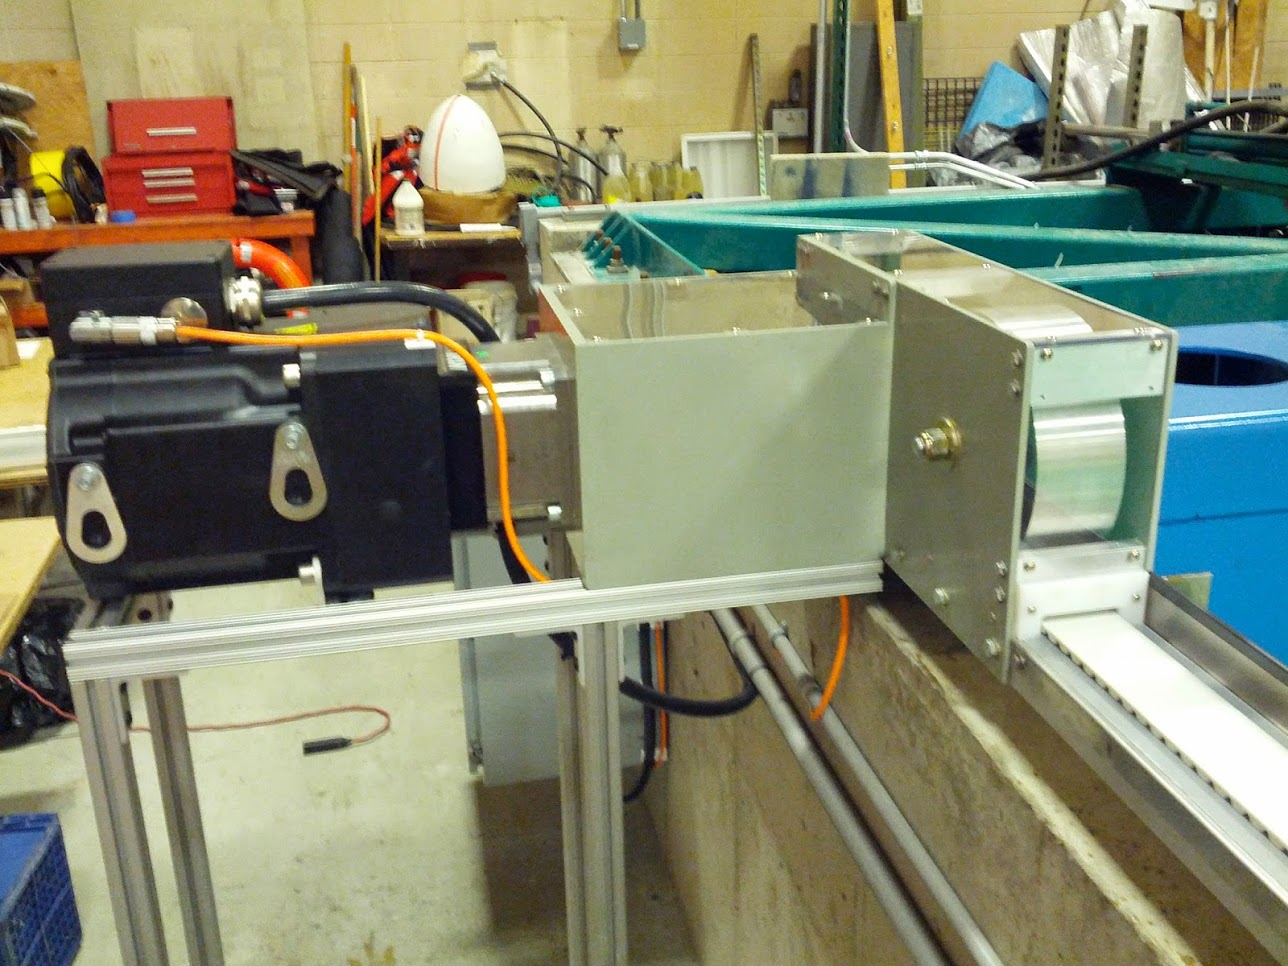
\includegraphics[clip, trim=0 0 0 1.5in, width=0.8\textwidth]{tow-servo}

    \caption{Upgraded tow system servo motor, gearbox, and custom-designed
        timing belt pulley housing.}

    \label{fig:tow-servo}
\end{figure}

A 7.5 cm wide steel-reinforced polyurethane timing belt was chosen as the new
drive member. The most robust timing belt profile---an ATL20---was chosen for
maximum stiffness per unit width. Custom timing belt and pulley housings were
designed to move both the upper and lower runs of the belt above the tank wall,
shortening the overall length, which when combined with the higher specific
stiffness belt increased the total drive member spring constant roughly by a
factor of 7.


\subsection{Data acquisition and onboard accessories}

The previous generation tow tank data acquisition (DAQ) system was based around
an onboard PC, powered by a set of four 12 V automotive batteries. This was done
to avoid the complexity of running power out to the carriage \cite{Darnell1996}.
The DAQ PC was accessed wirelessly via Windows Remote Desktop to control any DAQ
applications. The PC that sent the control signal to the inverter drive was a
separate machine, which meant users had to work with at least two interfaces to
specify DAQ and motion parameters. This also made it difficult to synchronize
motion with data acquisition, e.g., triggering data collection at a certain
location.

A new DAQ system was designed based around a National Instruments (NI) 9188
CompactDAQ Ethernet chassis. NI 9237, 9205, 9401, and 9411 modules were
installed for analog bridge, analog voltage, digital, and quadrature encoder
signals, respectively. A single CAT5e cable was dedicated for this system.
Additional cables were run for the EtherCAT and Internet connectivity on the
carriage. An 8-port Ethernet-serial server was installed for accessing serial
devices, e.g., the Nortek Vectrino+, described later. For measuring carriage
speed, and therefore inflow velocity, a Renishaw LM15 linear encoder with 10
$\mu$m resolution was installed and connected to the NI 9411 module. Networking,
power, and control signal cables were run through an igus cable carrier,
installed along the ``slave'' or $+y$ side of the tank.

Requirements for onboard power were derived from the goal of fully automating
both motion and data acquisition. It was also determined that the UNH ME
department's high frame rate particle image velocimetry (HFR-PIV) system would
be used on the carriage at some point, which included laser power supplies and a
laser chiller that could not be powered by the previous generation's isolated
battery/inverter system.

An onboard electronics cabinet was designed by Minarik, Inc. as part of the
upgraded motion system. A 45 amp, 120 VAC circuit and 20 amp, 240 VAC single
phase power cable were run through the cable carrier to power outlets on the
side of the onboard electronics cabinet. An additional 240 VAC three-phase
supply was connected to a Kollmorgen AKD servo drive, also installed in the
cabinet, which was sized to power a servo motor to control turbine shaft
position and speed. The AKD drive's digital outputs were setup for triggering
instrumentation, e.g., the NI 9188 chassis, via the main motion controller.


\section{Upgraded turbine test bed}

For this work, the turbine test bed was kept mostly intact, but modified for
fully-automated operation. To reduce low frequency resonance in the frame caused
by turbine side forces, and help redistribute some of the streamwise force from
turbines towed at higher speeds, two pairs of steel guy wires were added. These
solutions were chosen based on a finite element analysis (FEA) of the turbine
mounting frame, which showed more improvement regarding stiffening in the
desired directions compared to simply adding 45 degree flat bar braces in the
corner joints. To ensure drag from the outer guy wires was included in the
overall streamwise force measurement, an additional set of linear bearings was
added to the carriage for their connection.

Summaries of turbine test bed sensors and instrumentation are presented in
Table~\ref{tab:sensors} and Table~\ref{tab:instrumentation}, respectively. A
drawing and photo of the test bed are shown in
Figure~\ref{fig:turbine-test-bed}. Details on each subsystem are presented in
following sections.

\begin{table}
    \centering
    \begin{tabular}{c|c|c|c}
        Measured quantity & Device type & Mfg. \& model & Nominal accuracy \\
        \hline
        Carriage position & Linear encoder & Renishaw LM15 & 10 $\mu$m/pulse \cite{RenishawLM15}\\
        Turbine angle & Servo encoder output & Kollmorgen AKD & 10$^5$ pulse/rev \cite{KollmorgenAKD}\\
        Turbine torque & Rotary transducer & Interface T8-200 & $\pm$0.5 Nm \cite{InterfaceT8}\\
        Turbine torque (2) & Load cell (\& arm) & Sentran ZB3-200 & $\pm$0.2 Nm \cite{SentranZB}\\
        Drag force, left & Load cell & Sentran ZB3-500 & $\pm$0.6 N \cite{SentranZB}\\
        Drag force, right & Load cell & Sentran ZB3-500 & $\pm$0.6 N \cite{SentranZB}\\
        Fluid velocity & ADV & Nortek Vectrino+ & $\pm$0.5\% $\pm$1 mm/s \cite{NortekVectrino}\\
    \end{tabular}

    \caption{Turbine test bed sensor details. Note that ``(2)'' denotes a
        secondary redundant measurement. ``Turbine torque (2)'' nominal accuracy
        estimated by combining load cell accuracy and arm machining tolerances ($\pm
        1 \times 10^{-4}$ m) as root-sum-square.}

    \label{tab:sensors}
\end{table}

\begin{table}
    \centering
    \begin{tabular}{c|c|c}
        Measured quantity & Device type & Mfg. \& model \\
        \hline
        Carriage position & Differential counter & NI 9411 \\
        Carriage velocity (2) & Motion controller & ACS NTM \\
        Turbine angle & Differential counter & NI 9411 \\
        Turbine RPM (2) & Motion controller & ACS NTM \\
        Turbine torque & Analog voltage input & NI 9205 \\
        Turbine torque (2) & Analog bridge input & NI 9237 \\
        Drag force, left & Analog bridge input & NI 9237 \\
        Drag force, right & Analog bridge input & NI 9237 \\
    \end{tabular}

    \caption{Details of the instrumentation used to perform experiments with the
        turbine test bed. Note that ``(2)'' denotes a secondary redundant
        measurement.}

    \label{tab:instrumentation}
\end{table}

\begin{figure}
    \centering
    \begin{subfigure}[t]{\textwidth}
        \centering

        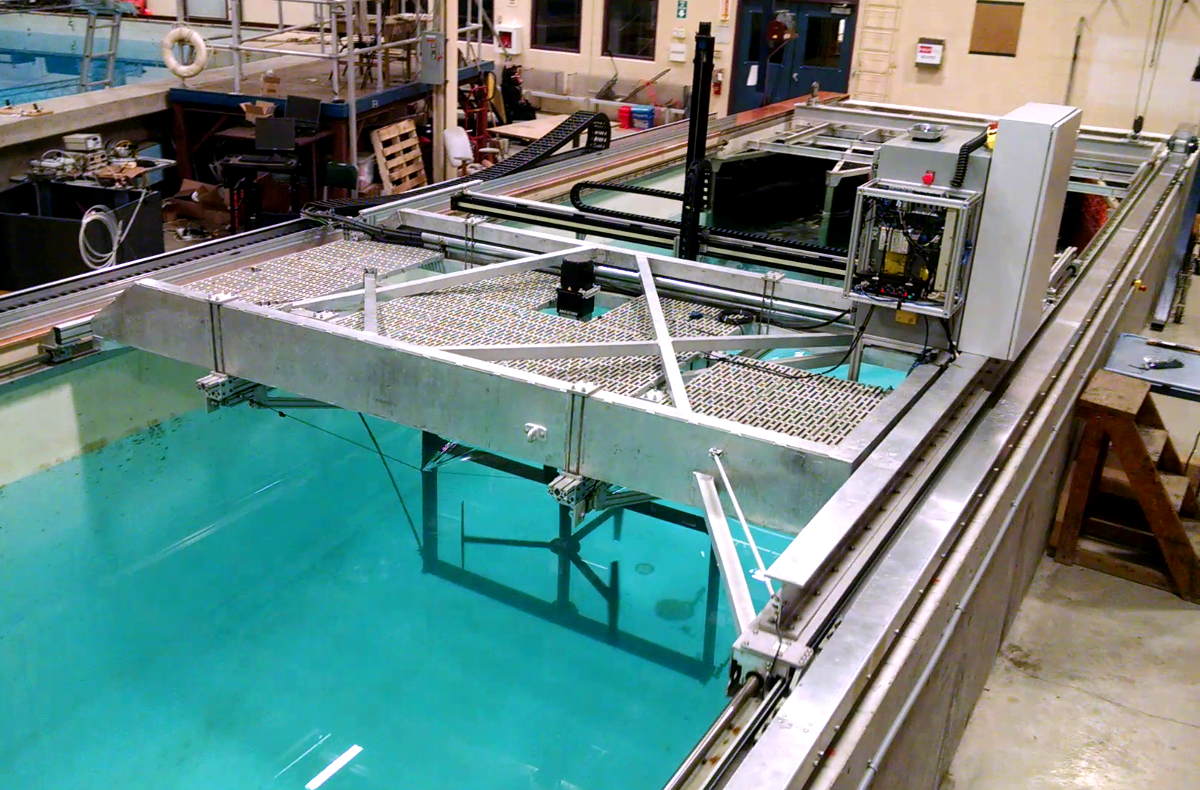
\includegraphics[width=0.75\textwidth]{figures/turbine-test-bed-photo}

        \caption{}

        \label{fig:turbine-test-bed-photo}
    \end{subfigure}

    \begin{subfigure}[t]{\textwidth}
        \centering

        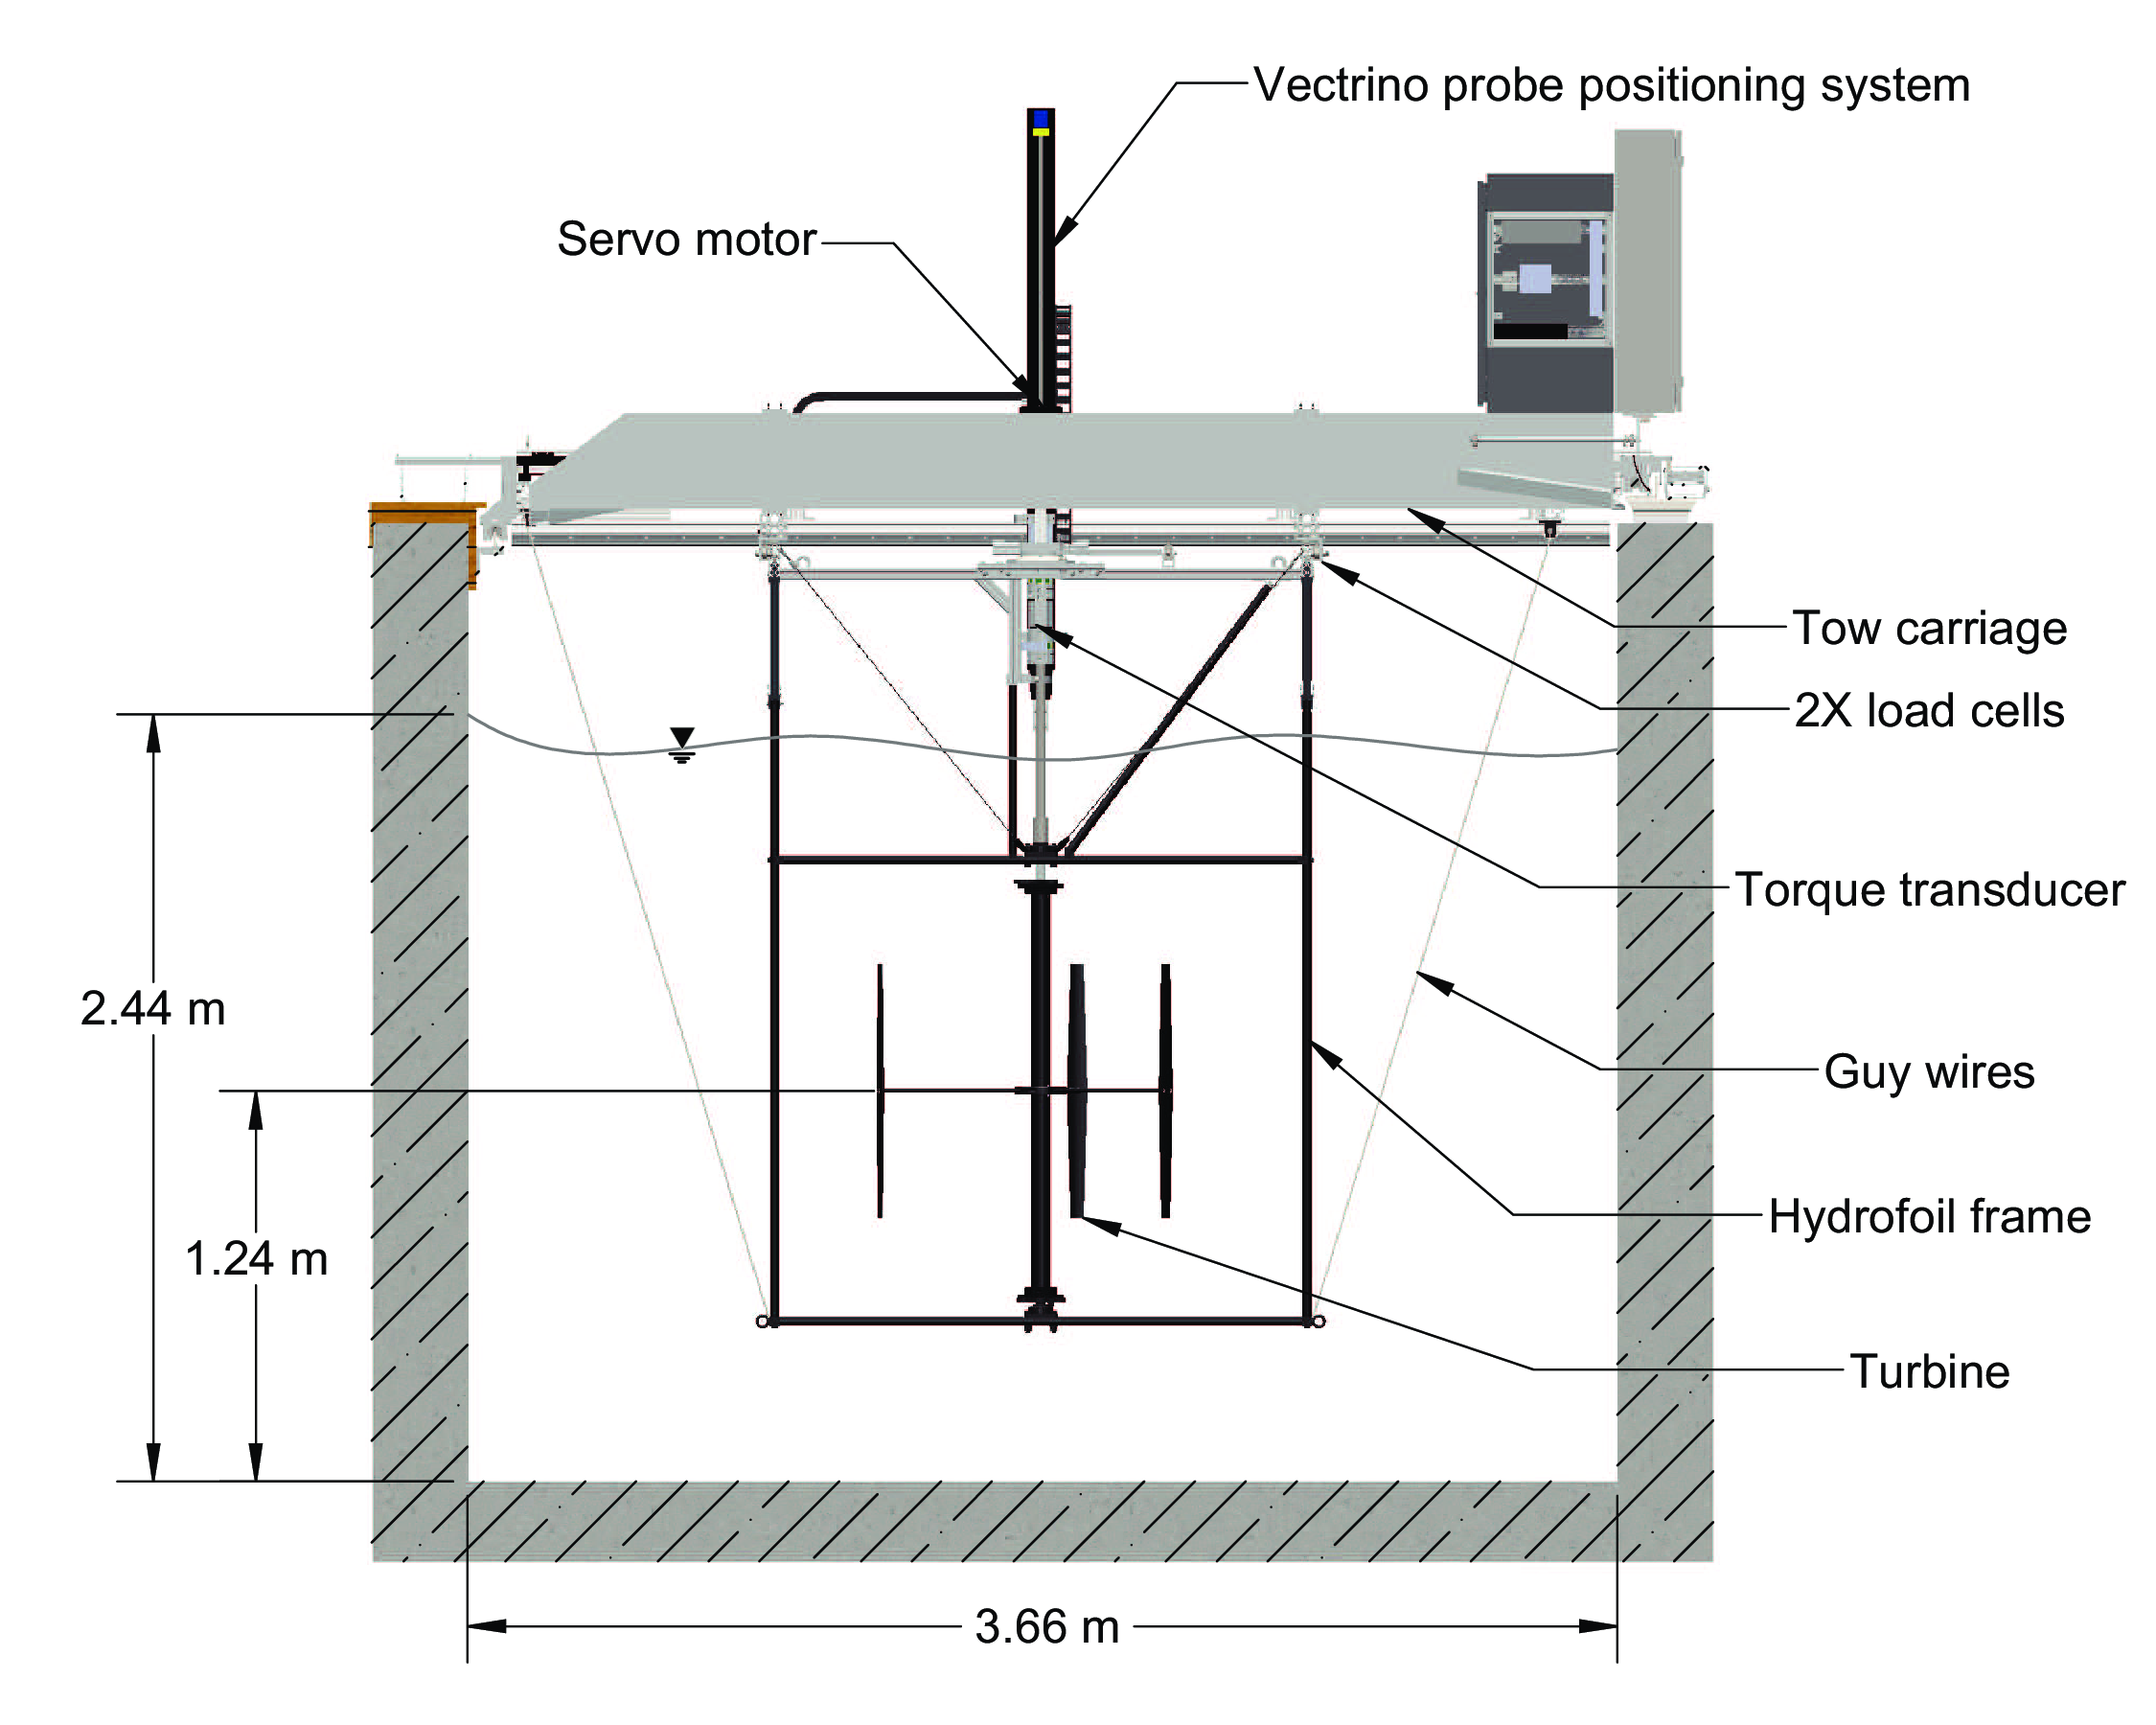
\includegraphics[width=0.85\textwidth]{turbine-test-bed-drawing}

        \caption{}

        \label{fig:turbine-test-bed-drawing}
    \end{subfigure}

    \caption{Turbine test bed photo (a) and drawing (b).}

    \label{fig:turbine-test-bed}
\end{figure}


\subsection{Turbine loading, speed control, torque, and drag measurement}

In order to control turbine shaft angular velocity, a Kollmorgen AKM62Q servo
motor and 20:1 ratio gearhead were added with a custom retrofit mounting plate
and housing. Two zero-backlash R+W EKH/300/B curved jaw couplings were added
above and below the rotary torque transducer. An additional torque measurement
system was added by mounting the servo/gearhead assembly to a slewing ring
bearing, and holding its mounting housing in place by a Sentran ZB3 200 lbf load
cell attached at a fixed distance by a 16 inch long arm. This system served as a
redundant torque measurement for values up to 200 Nm, and extended the maximum
torque range to approximately 360 Nm.

Turbine shaft angle was measured via the AKD drive's emulated encoder output,
set to $5 \times 10^3$ (pre-gearbox) or $1 \times 10^5$ (post-gearbox)
lines-per-rev in an A-quad-B configuration. This signal was sampled by either
the NI 9401 (experiments reported in Chapter~\ref{chap:RVAT-baseline}) or the NI
9411 (experiments reported in Chapters~\ref{chap:Re-dep} and \ref{chap:RM2})
modules. Shaft speed was computed by differentiating the angle time series with
a second order central difference scheme. A moving average filter $\sim$10
samples wide was applied to smooth the resulting $\omega$ time series such that
it agreed nearly identically with the shaft RPM measured by the servo motor's
resolver feedback as sampled by the motion controller.

The two drag slide assemblies for overall streamwise drag or thrust measurement
were retained from the previous setup, which is described in
\cite{Bachant2011-MS}. All turbine performance related signals were sampled by
modules in the NI 9188 CompactDAQ chassis at a 2 kHz sample rate.


\subsection{Wake measurement system}

In order to characterize turbine wakes, a Nortek Vectrino+ acoustic Doppler
velocimeter (ADV) was purchased with a Hubbard Fund grant from UNH. An ADV is
capable of measuring three components of velocity at a single point in space
(technically over a small volume), and the Vectrino+ was set to sample at 200
Hz. This system was considered desirable compared with hot wire or hot film
anemometry as it required no calibrations, and the sensor element is
significantly more robust. Spatial resolution is typically lower---the
Vectrino's measurement volume is 6 mm in diameter \cite{NortekVectrino}---but
this is still small compared with the typical length scale of a turbine model.
ADV was also preferable to laser Doppler velocimetry (LDV) in this case since
the tow carriage is a high vibration environment, which would make LDV alignment
a challenge.

\nomenclature{ADV}{Acoustic Doppler velocimeter.}

A $y$--$z$ axis positioning system was designed for the Vectrino probe. This
system consisted of two Velmex BiSlide linear stages---the $y$-axis driven by
belt and the $z$-axis by ball screw. Both drive systems were powered by stepper
motors with approximately 0.001 inch resolution. These motors were driven by an
ACS UDMlc EtherCAT drive, connected to the tow tank's main motion controller for
integrated synchronous motion.

When operating the Vectrino, the tank was seeded with 11 $\mathrm{\mu}$m mean
diameter hollow glass spheres. Seeding was added along the tank length,
generally at the surface, and was mixed by towing the turbine through the tank.
This process was repeated until the Vectrino's signal-to-noise ratio (SNR) was
approximately above 12 dB. Seeding was added throughout experiments as
necessary---totaling approximately 1--5 cups (dry) per day. Note that while
acquiring ADV data the $y$- and $z$-axis stepper drive had to be disabled to
reduce noise. The axes were re-enabled to position the probe before each run.


\subsection{Software}

Software was developed to automate the entire turbine testing process. Dubbed
TurbineDAQ, the desktop application was written in Python due to its reputation
as a good ``glue'' language for systems integration. The graphical user
interface (GUI), shown in Figure~\ref{fig:TurbineDAQ}, was built using the PyQt
bindings to the Qt framework. Communication with the tow tank's motion
controller, data acquisition system, and ADV were integrated into a single
application. This, combined with the ability to load and automatically execute
test matrices in comma-separated value (CSV) format, allowed for experiments
consisting of thousands of tows, where the previous generation test bed could
only realistically achieve around 100. Note that the software was developed
after the experiments in Chapter~\ref{chap:RVAT-baseline}, for which turbine tip
speed ratio, Vectrino positioning, and data collection parameters were input
manually. However, TurbineDAQ was developed before and employed for both the
larger experiments described in Chapter~\ref{chap:Re-dep} and
Chapter~\ref{chap:RM2}.

\nomenclature{GUI}{Graphical user interface.}

\begin{figure}
    \centering

    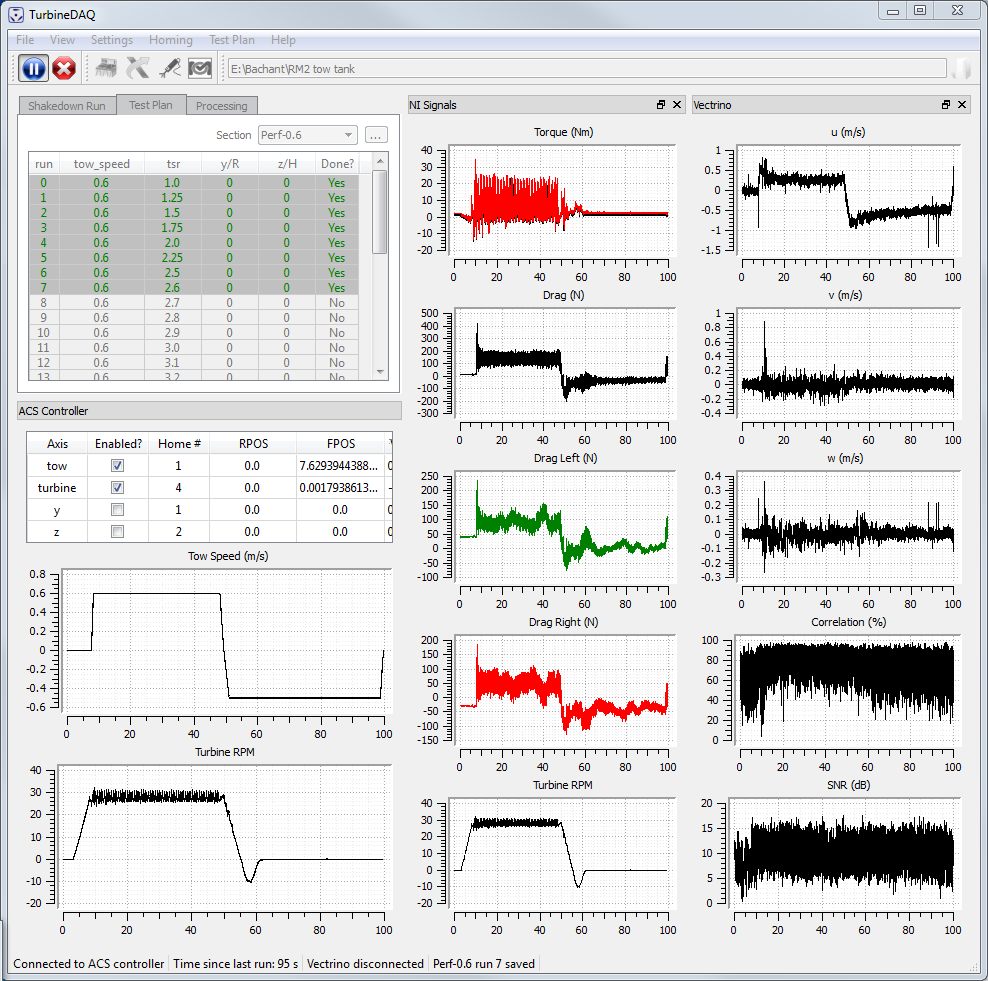
\includegraphics[width=0.95\textwidth]{TurbineDAQ}

    \caption{TurbineDAQ turbine test bed experiment automation software
    graphical interface.}

    \label{fig:TurbineDAQ}
\end{figure}


\subsection{Tare drag and torque compensation}

The drag and torque measurement systems were set up in such a way that raw
measurements for drag would include all submerged gear and torque would include
all friction below the transducer along with the turbine shaft torque. To
compensate, tare torque and drag runs were performed to measure the shaft
bearing friction torque and turbine mounting frame drag, respectively. Tare drag
runs were performed for each tow speed in each experiment, for which the mean
value was subtracted in data processing to estimate rotor drag alone. Tare
torque runs were performed by rotating the turbine shaft (without blades) in air
at constant angular velocity for a specified duration, over the range of angular
velocities used throughout the experiment. Tare torque was then fit with a
linear regression versus shaft angular velocity, and added to the measured
turbine torque in post-processing.


\subsection{Synchronization of instrumentation subsystems}

The three data acquisition instrumentation subsystems---motion controller, NI
DAQ (performance measurements), and Vectrino+ (wake velocity
measurements)---were set to begin sampling at precisely the same time each run,
after being triggered by a TTL pulse created by the motion controller. This
strategy retains synchronization for all performance signal samples (tow speed,
torque, drag, angular velocity), ensuring precise calculation of, e.g., power
coefficient. Since there is also synchronization of the initial sample from each
three subsystems, correlation of events in the performance and wake signals is
also possible.

\nomenclature{DAQ}{Data acquisition.}


\subsection{Calibrations}

Factory calibrations for all instrumentation were used for the experiments
described in Chapters~\ref{chap:RVAT-baseline} and \ref{chap:Re-dep}. The drag
slide and torque arm assemblies were calibrated out of the tank using the
fixtures shown in Figure~\ref{fig:calibration-fixtures}, in which a Sentran ZB3
500 lbf capacity load cell and indicator were used for input values. The
reference load cell and indicator were calibrated as a full system from the
factory and remained connected to each other at all times. The drag slide and
torque arm fixtures were loaded incrementally using a 3/4-16 inch threaded rod,
nut, and self-lubricating thrust bearing.

\begin{figure}
    \centering
    \begin{subfigure}{0.9\textwidth}
        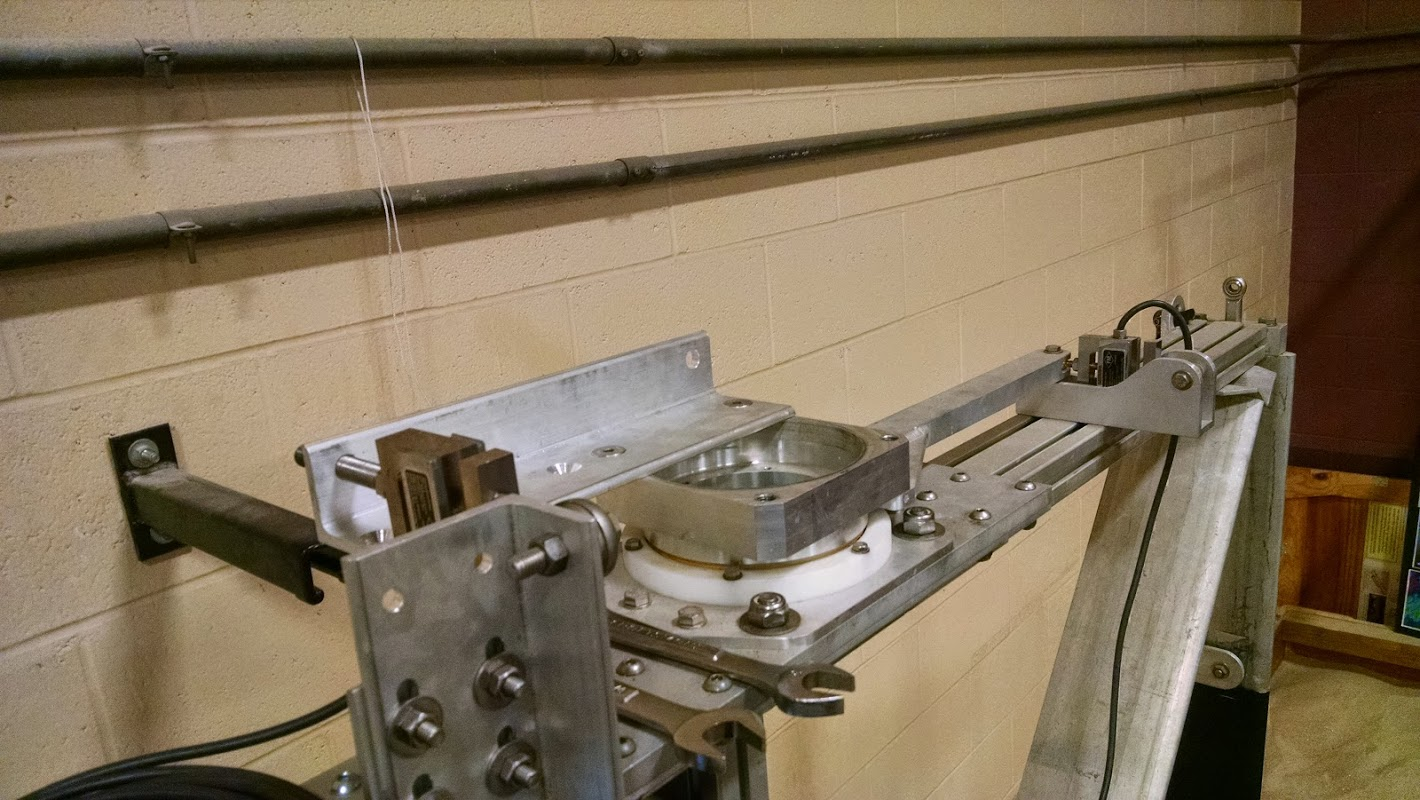
\includegraphics[clip, trim=0 0 0 3in,
        width=\textwidth]{torque-arm-calibration} \caption{}
    \end{subfigure}

    \begin{subfigure}{0.9\textwidth}
        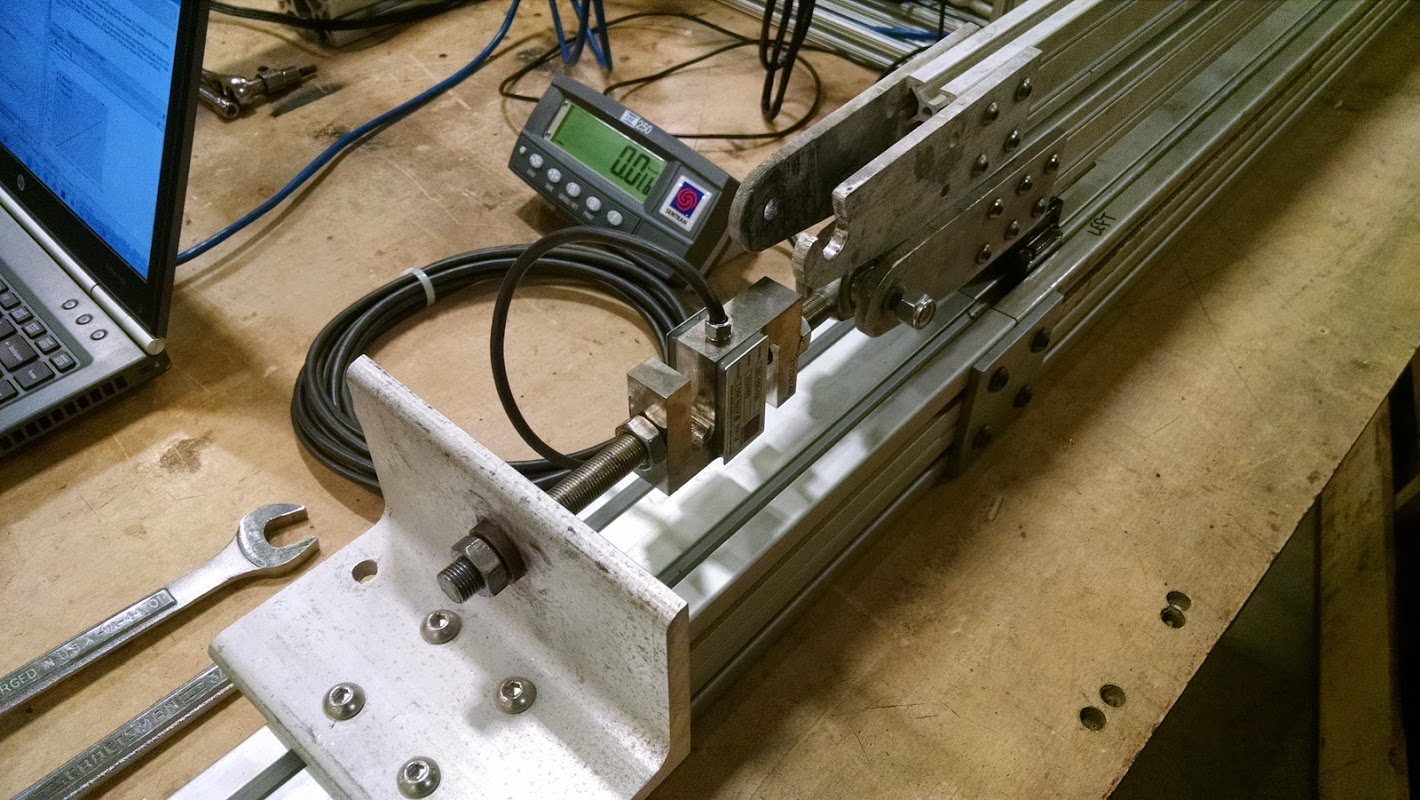
\includegraphics[width=\textwidth]{drag-slide-calibration}
        \caption{}
    \end{subfigure}

    \caption{Torque arm (a) and drag slide (b) calibration fixtures. Note that
        the same load cell, indicator, and thrust bearing are used for both setups.}

    \label{fig:calibration-fixtures}
\end{figure}

Before the RM2 experiment described later in Chapter~\ref{chap:RM2}, traceable
calibration certificates were obtained for the Interface T8-200 torque
transducer and NI 9205 and NI 9237 modules. In 2014, the drag slide and torque
arm assemblies were recalibrated using the same fixture and Sentran ZB3 load
cell and indicator described above, for which a new traceable calibration
certificate was obtained. Values before and after the recalibration are
presented in Table~\ref{tab:calibrations}.

\nomenclature{RM2}{Reference Model 2.}

\begin{table}
    \centering
\begin{tabular}{c|c|c|c}
    Signal & Calibration 1 & Calibration 2 & Difference \\
    \hline
    Torque trans. & 40.0000 Nm/V & 39.8380 Nm/V & -0.4 \% \\
    Torque arm & 122531 Nm/V/V & 123437 Nm/V/V & 0.7 \% \\
    Drag left & 743104 N/V/V & 742830 N/V/V & -0.1 \% \\
    Drag right & 740137 N/V/V & 742400 N/V/V & 0.3 \% \\
\end{tabular}
    \caption{Calibration slopes used for experimental measurements. Calibration
        1 was used for the experiments described in Chapter~\ref{chap:RVAT-baseline}
        and Chapter~\ref{chap:Re-dep}. Calibration 2 was used for those in
        Chapter~\ref{chap:RM2}.}

    \label{tab:calibrations}
\end{table}


\section{Determining tank settling time}

For each experiment, sample turbine tows were performed at each speed to
determine the amount of time taken between runs such that the tank has settled
adequately, i.e., background turbulence and any large scale mean flows have been
dissipated. This was assessed by towing the turbine, bringing the carriage back
to mid-tank, and allowing the Vectrino to continue recording velocity data,
monitoring the mean and standard deviation of the signals.

Turbulence intensity tended to decay quickly, while the lower frequency
fluctuations were damped with the help of the tank's ``beach,'' designed for
absorbing waves created by the paddle-style wavemaker. Settling times ranged
from 140 seconds for tows at 0.3 m/s up to 360 seconds for those at 1.4 m/s.
These values were then included in the experiment configuration---one value for
each tow speed, to be used by TurbineDAQ as wait times between automated runs.


\section{Blockage}

Placing a turbine in a confined environment such as a towing tank will force
flow through the turbine at higher velocity compared with a free case, where
streamlines are allowed to diverge. Consequently, higher levels of blockage will
lead to increased turbine performance, and a shift in optimal operating
parameters, i.e., tip speed ratio. In order to for experiments to be relevant to
others in the literature, blockage effects must either be corrected for, or the
blockage ratio should be kept to a typical value seen in other studies.

Most numerical models have the ability to include finite domains or walls, which
makes uncorrected applicable to validation; applying blockage corrections may
even complicate validation efforts. Furthermore, blockage will be non-zero in
most MHK cases, where turbines are placed in rivers or channels, the effects of
which need to be predicted as well. Since a definitive blockage correction for
CFTs has not yet been established \cite{Cavagnaro2014, Dossena2015}, and a 1
m\textsuperscript{2} turbine creates a reasonably low blockage---on the order of
10\%---no corrections were applied.

\nomenclature{MHK}{Marine hydrokinetic.}


\section{Turbine models}

Two physical turbine models were designed and built. The first was intended to
be a geometrically simple---not necessarily very efficient---high-solidity
turbine. This simplicity was achieved with symmetrical foil profiles, square
frontal rotor area, and a rectangular blade planform. This turbine was
constructed from materials donated by Lucid Energy Technologies, LLP, and dubbed
the ``Reference Vertical-Axis Turbine'' or UNH-RVAT.

The second turbine was designed and built as part of a measurement task for
Sandia National Laboratories (SNL), in collaboration with the US Department of
Energy (DOE), which is described in more detail later in Chapter~\ref{chap:RM2}.
The so-called ``Reference Model 2'' (RM2) was developed by SNL to be a standard
cross-flow turbine for which modelers could validate their predictions
\cite{Neary2014}. The RM2 was designed using Sandia's CACTUS vortex line code
\cite{Barone2011}, and its low-to-medium solidity made it a nice complement to
the UNH-RVAT for testing the robustness of numerical models to varying solidity.


\subsection{UNH-RVAT}

The UNH-RVAT turbine was constructed from straight 14 cm chord length NACA 0020
extrusions, used for both the blades and struts. Blades were mounted at
mid-chord, mid-span, and zero preset pitch, with a length or height of 1 m and
placed at 1 m diameter, giving the rotor an aspect ratio of unity. These
parameters gave the rotor a relatively high solidity $Nc/(\pi D) = 0.13$ and a
large chord-to-radius ratio $c/R = 0.28$.

The support struts were also constructed from 14 cm chord NACA 0020 profiles,
and attach the turbine to a 9.5 cm diameter shaft. A drawing of the turbine
rotor is shown in Figure~\ref{fig:rvat-drawing} and CAD models are available
from \cite{Bachant2014-RVAT-CAD}. The turbine is shown outside of the tank
installed in the test bed mounting frame in Figure~\ref{fig:rvat-photo}.

\begin{figure}
    \centering
    \begin{subfigure}{0.49\textwidth}
        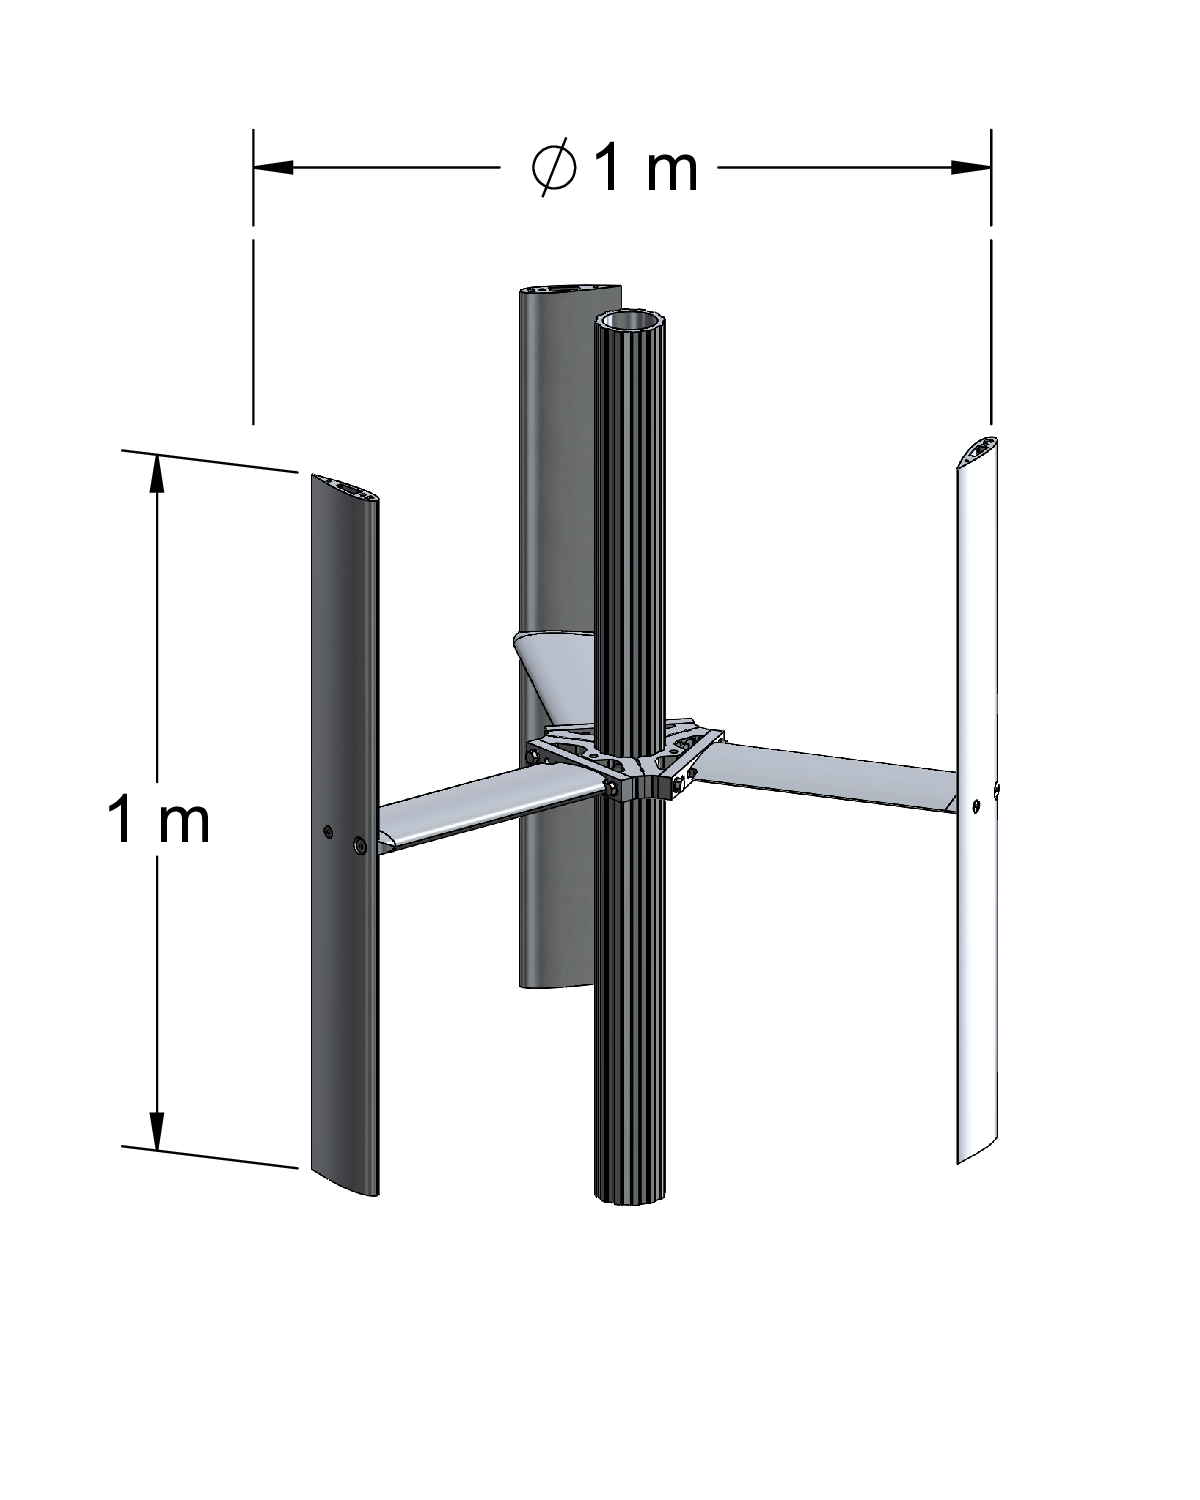
\includegraphics[width=\textwidth]{unh-rvat-drawing}
        \caption{}
        \label{fig:rvat-drawing}
    \end{subfigure}
    \begin{subfigure}{0.47\textwidth}
        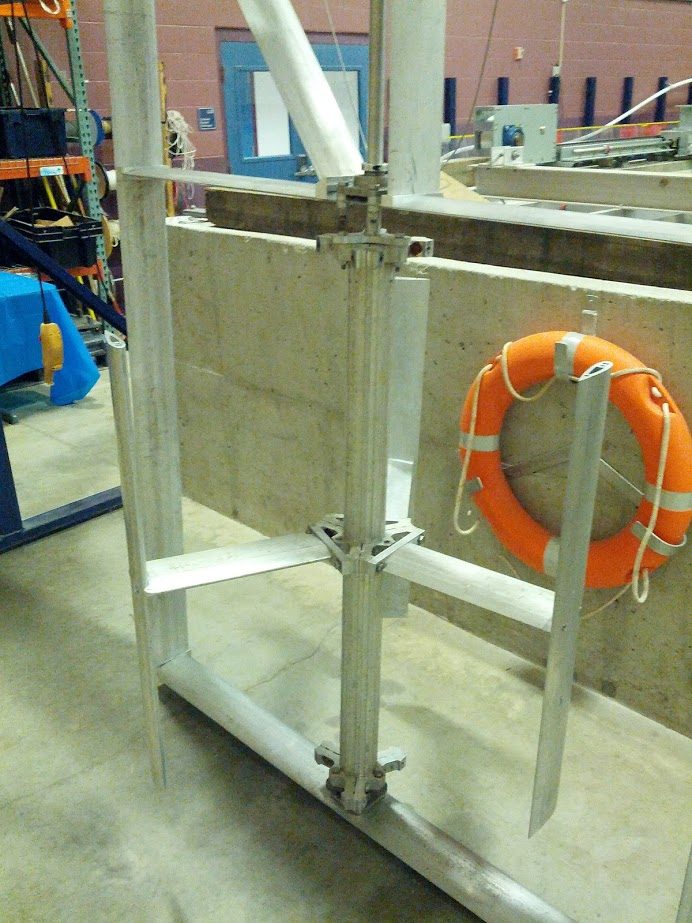
\includegraphics[width=\textwidth]{unh-rvat-photo}
        \caption{}
        \label{fig:rvat-photo}
    \end{subfigure}

    \caption{Drawing (a) and photo (b) of the UNH-RVAT vertical-axis cross-flow
        turbine. Note that the upper and lower mounting flanges (and the area of the
        shaft they cover) have been excluded in the drawing. These were included in
        the tare drag measurements for the experiments in Chapter~\ref{chap:Re-dep},
        but excluded for those in Chapter~\ref{chap:RVAT-baseline}.}

    \label{fig:unh-rvat}
\end{figure}


\subsection{DOE/SNL RM2}

The RM2 rotor was designed as a 1:6 scale model of that described in the RM2
``rev 0'' design report \cite{Barone2011}, with the exception of the shaft
diameter, which was scaled from the SAFL RM2 shaft \cite{Hill2014}. The hub
design is also similar to the SAFL model. A drawing of the turbine design is
shown in Figure~\ref{fig:rm2-drawing} and a photo of the RM2 installed in the
turbine test bed mounting frame is shown in Figure~\ref{fig:rm2-photo}. The
rotor has tapered blades with $c/R=0.12$ at the roots (mid-span) and $c/R=0.07$
at the tips, which uniquely gives it a medium-high solidity for a wind turbine
and low solidity for an MHK turbine. The RM2 is discussed in more detail in
Chapter~\ref{chap:RM2}.

\begin{figure}
    \centering

    \begin{subfigure}{0.45\textwidth}
        \centering
        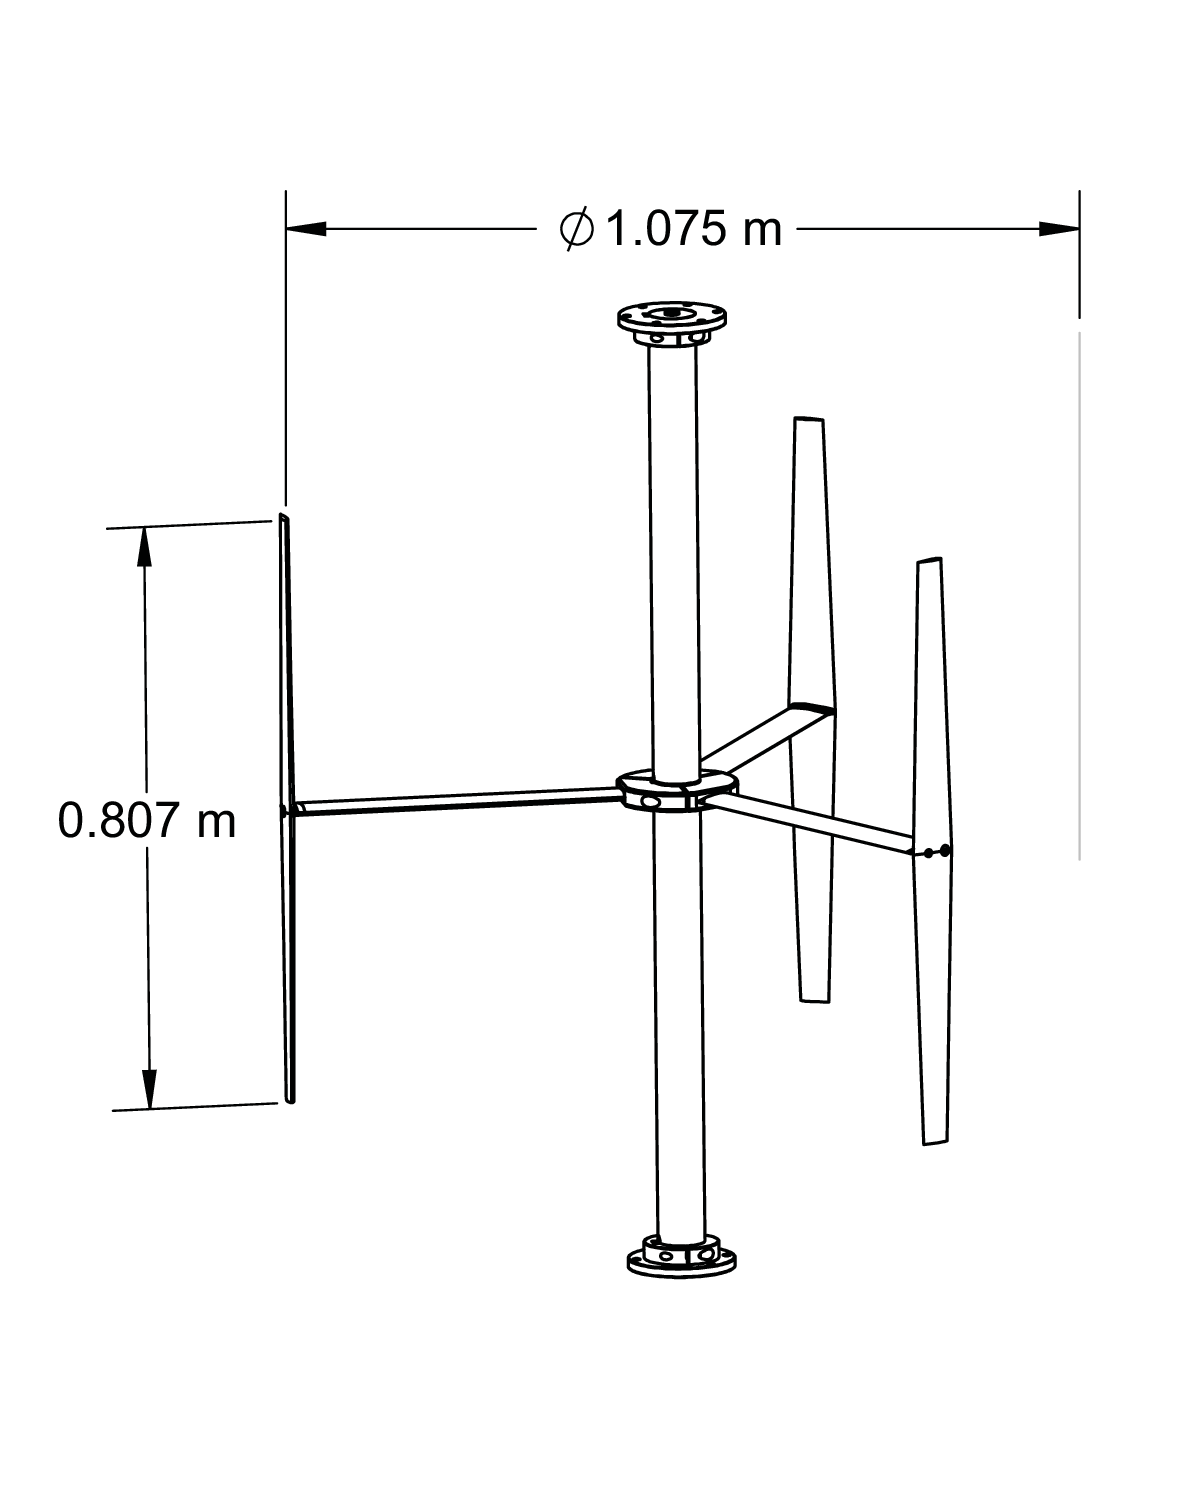
\includegraphics[clip, trim=0 0.5in 0 0.6in, width=\textwidth]{rm2-drawing}
        \caption{}
        \label{fig:rm2-drawing}
    \end{subfigure}
    \begin{subfigure}{0.41\textwidth}
        \centering
        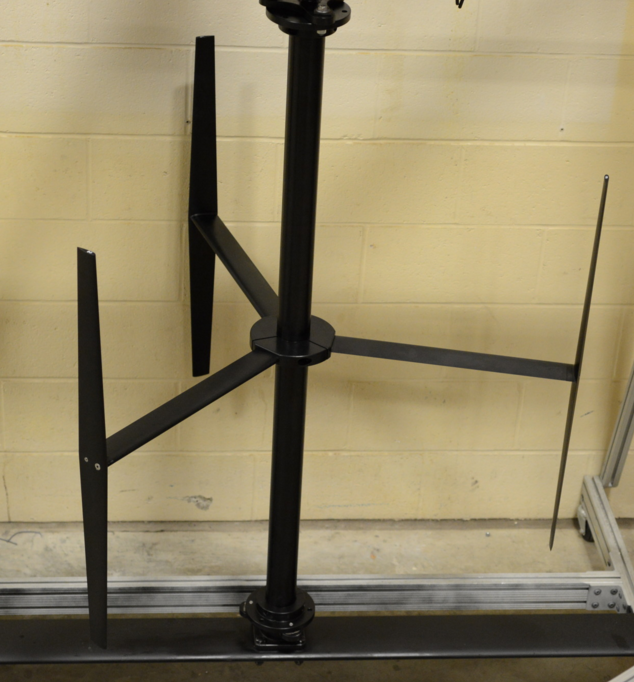
\includegraphics[width=\textwidth]{rm2-photo}

        \caption{}
        \label{fig:rm2-photo}
    \end{subfigure}

    \caption{Drawing (a) and photo (b) of the 1:6 RM2 scaled physical model cross-flow turbine.}
    \label{fig:rm2}
\end{figure}


\section{Summary and conclusions}

An upgraded test bed for measuring the performance and near-wake flows of large
laboratory scale ($O(1)$ m\textsuperscript{2} frontal area) cross-flow turbines
was developed for the UNH tow tank. To acquire adequate amounts of data and to
achieve significant lengths of steady state operation with a limited tank
length, the tow tank's linear motion, control, and data acquisition systems had
to be redesigned, rebuilt, and upgraded to allow fully automated operation,
along with higher carriage speed and acceleration. Integrating carriage,
turbine, and Vectrino probe positioning, along with synchronized data
acquisition from performance measurement, Vectrino, and motion controller
systems increased the number of tows possible per experiment by essentially an
order of magnitude, while simplifying data processing and increasing data
quality and repeatability. CAD files for the tow tank and turbine test bed are
available from~\cite{Bachant2016-tow-tank-CAD}.

\nomenclature{UNH}{University of New Hampshire.}
\nomenclature{UNH-RVAT}{University of New Hampshire Reference Vertical-Axis
Turbine.}
\nomenclature{CAD}{Computer-aided design.}

Two turbine models were designed and fabricated. The UNH-RVAT turbine was
designed to be more geometrically simple, but higher solidity, while the RM2
turbine is lower solidity, with tapered blades. The differences between these
rotors provide an opportunity for direct comparison within the same experimental
setup, and will provide validation data to test numerical models' predictive
capabilities with varying levels of flow curvature (from higher $c/R$) and end
effects (blade aspect ratio and taper).

% Chapter on RVAT baseline experiments
\chapter{Baseline experimental characterization of a high solidity cross-flow
turbine}\label{chap:RVAT-baseline}

As an initial baseline experiment with the turbine test bed, the performance and
near-wake velocity of the high solidity UNH-RVAT were measured. Note that the
results presented here have been published in \cite{Bachant2013,
    Bachant2015-JoT}.

The first task was to assess the rotor's characteristic performance (power and
drag coefficient versus tip speed ratio) curves. Next, a typical operating set
point tip speed ratio was established, at which the near-wake was examined in
detail to gain insight into the mechanisms that improve CFT wake recovery rates
compared with AFTs (allowing closer spacing, \emph{cf.} \cite{Kinzel2012}) or
other axisymmetric turbulent wakes, with the ultimate goal that these mechanisms
can be replicated in simpler models for use in simulations of large turbine
arrays, where resolving actual turbine geometry is prohibitively expensive. The
ability of one such model---an actuator disk inside a Reynolds-Averaged
Navier--Stokes (RANS) simulation---to predict those defining characteristics was
also assessed.

The dominant scales within the turbine's near-wake were evaluated for their
relative importance, loosely following the conceptual framework presented in
Chamorro \etal \cite{Chamorro2012b}, where the turbine was treated as an
``active filter.'' However, by extending this concept it should be cautioned
that this filter could also be nonlinear, i.e., the spectral modifications of
the inflow are dependent on the spectral distribution itself, not a
superposition of effects at each individual scale. It is also expected that a
CFT will introduce even stronger large (turbine) scale variance into the flow,
due to its cyclical forcing from oscillatory blade angles of attack and relative
velocity. The experiments presented here were performed in a towing tank,
providing a very low turbulence intensity inflow (at least as low as the
instrumentation noise floor), which provides an excellent baseline case for
spectral content added to the flow by the turbine, without any modulation of a
turbulent inflow spectra.

Previous detailed experimental studies with CFTs were generally limited in terms
of Reynolds number due to small geometric scale. On the other hand, as expected,
large-scale measurements were typically performed with lower resolution
instrumentation, and with less control of inflow conditions
\cite{Vermeulen1979}. Brochier \etal~\cite{Brochier1986} employed laser-Doppler
velocimetry (LDV) to acquire detailed flow measurements of a small-scale,
quasi-2-D CFT in dynamic stall. Their study was similar in scope to the work
presented here, but was conducted at very low Reynolds number---approximately
two orders of magnitude smaller than the study presented here. More recently,
Tescione \etal~\cite{Tescione2014} performed a detailed experimental campaign,
using particle image velocimetry to illuminate vortex structures in the wake,
and how these interact with each other. However, the question still remains as
to why the CFT wake would recover more quickly than that of an AFT. The study
reported here also examined the three-dimensionality of the wake, as turbine
``end effects'' will no doubt affect interaction with the free stream.

To summarize, the goals of this experiment were:
\begin{enumerate}
    \item To identify the essential features of the near-wake of a cross-flow
    turbine.
    
    \item To assess the relative importance of mean and turbulent dynamics on the
    transport of momentum and kinetic energy in the wake.
    
    \item To compare the measured CFT wake to numerical predictions from a
    uniform actuator disk force parameterization implemented inside a RANS
    model, to evaluate its prospects for representing CFTs in array simulations.
\end{enumerate}


\section{Experimental test plan}

All experiments were performed at a tow speed of 1 m/s, resulting in a Reynolds
number based on turbine diameter of $Re_D = U_\infty D /\nu = 1 \times 10^6$, or
an approximate blade chord Reynolds number of $Re_c \approx \lambda U_\infty
c/\nu = 2.7 \times 10^5$ for $\lambda=1.9$, where tip speed ratio $\lambda
\equiv \omega D / (2 U_\infty)$. Note that this Reynolds number is high enough
to be considered operating in a $Re$-independent regime \cite{Bravo2007,
    Bachant2014, Bachant2016-Energies}, which is examined in more detail in
Chapter~\ref{chap:Re-dep}.

The performance of the turbine was measured first by operating at a range of tip
speed ratios, which were held constant during individual tows, and varied from
almost zero to just above that where power becomes negative, i.e., where the
motor has to drive the rotor. From the $C_P$--$\lambda$ curve, the optimal tip
speed ratio $\lambda_0$ was selected for characterizing the wake at one rotor
diameter downstream of the rotor axis. The flow measurements mapped out the
upper half of the turbine wake over 3 m in the spanwise direction, centered
within the 3.66 m tank width, the coordinate system and locations for which are
shown in Figure~\ref{fig:RVAT-baseline-wake-coordinates}.

\begin{figure}
    \centering
    
    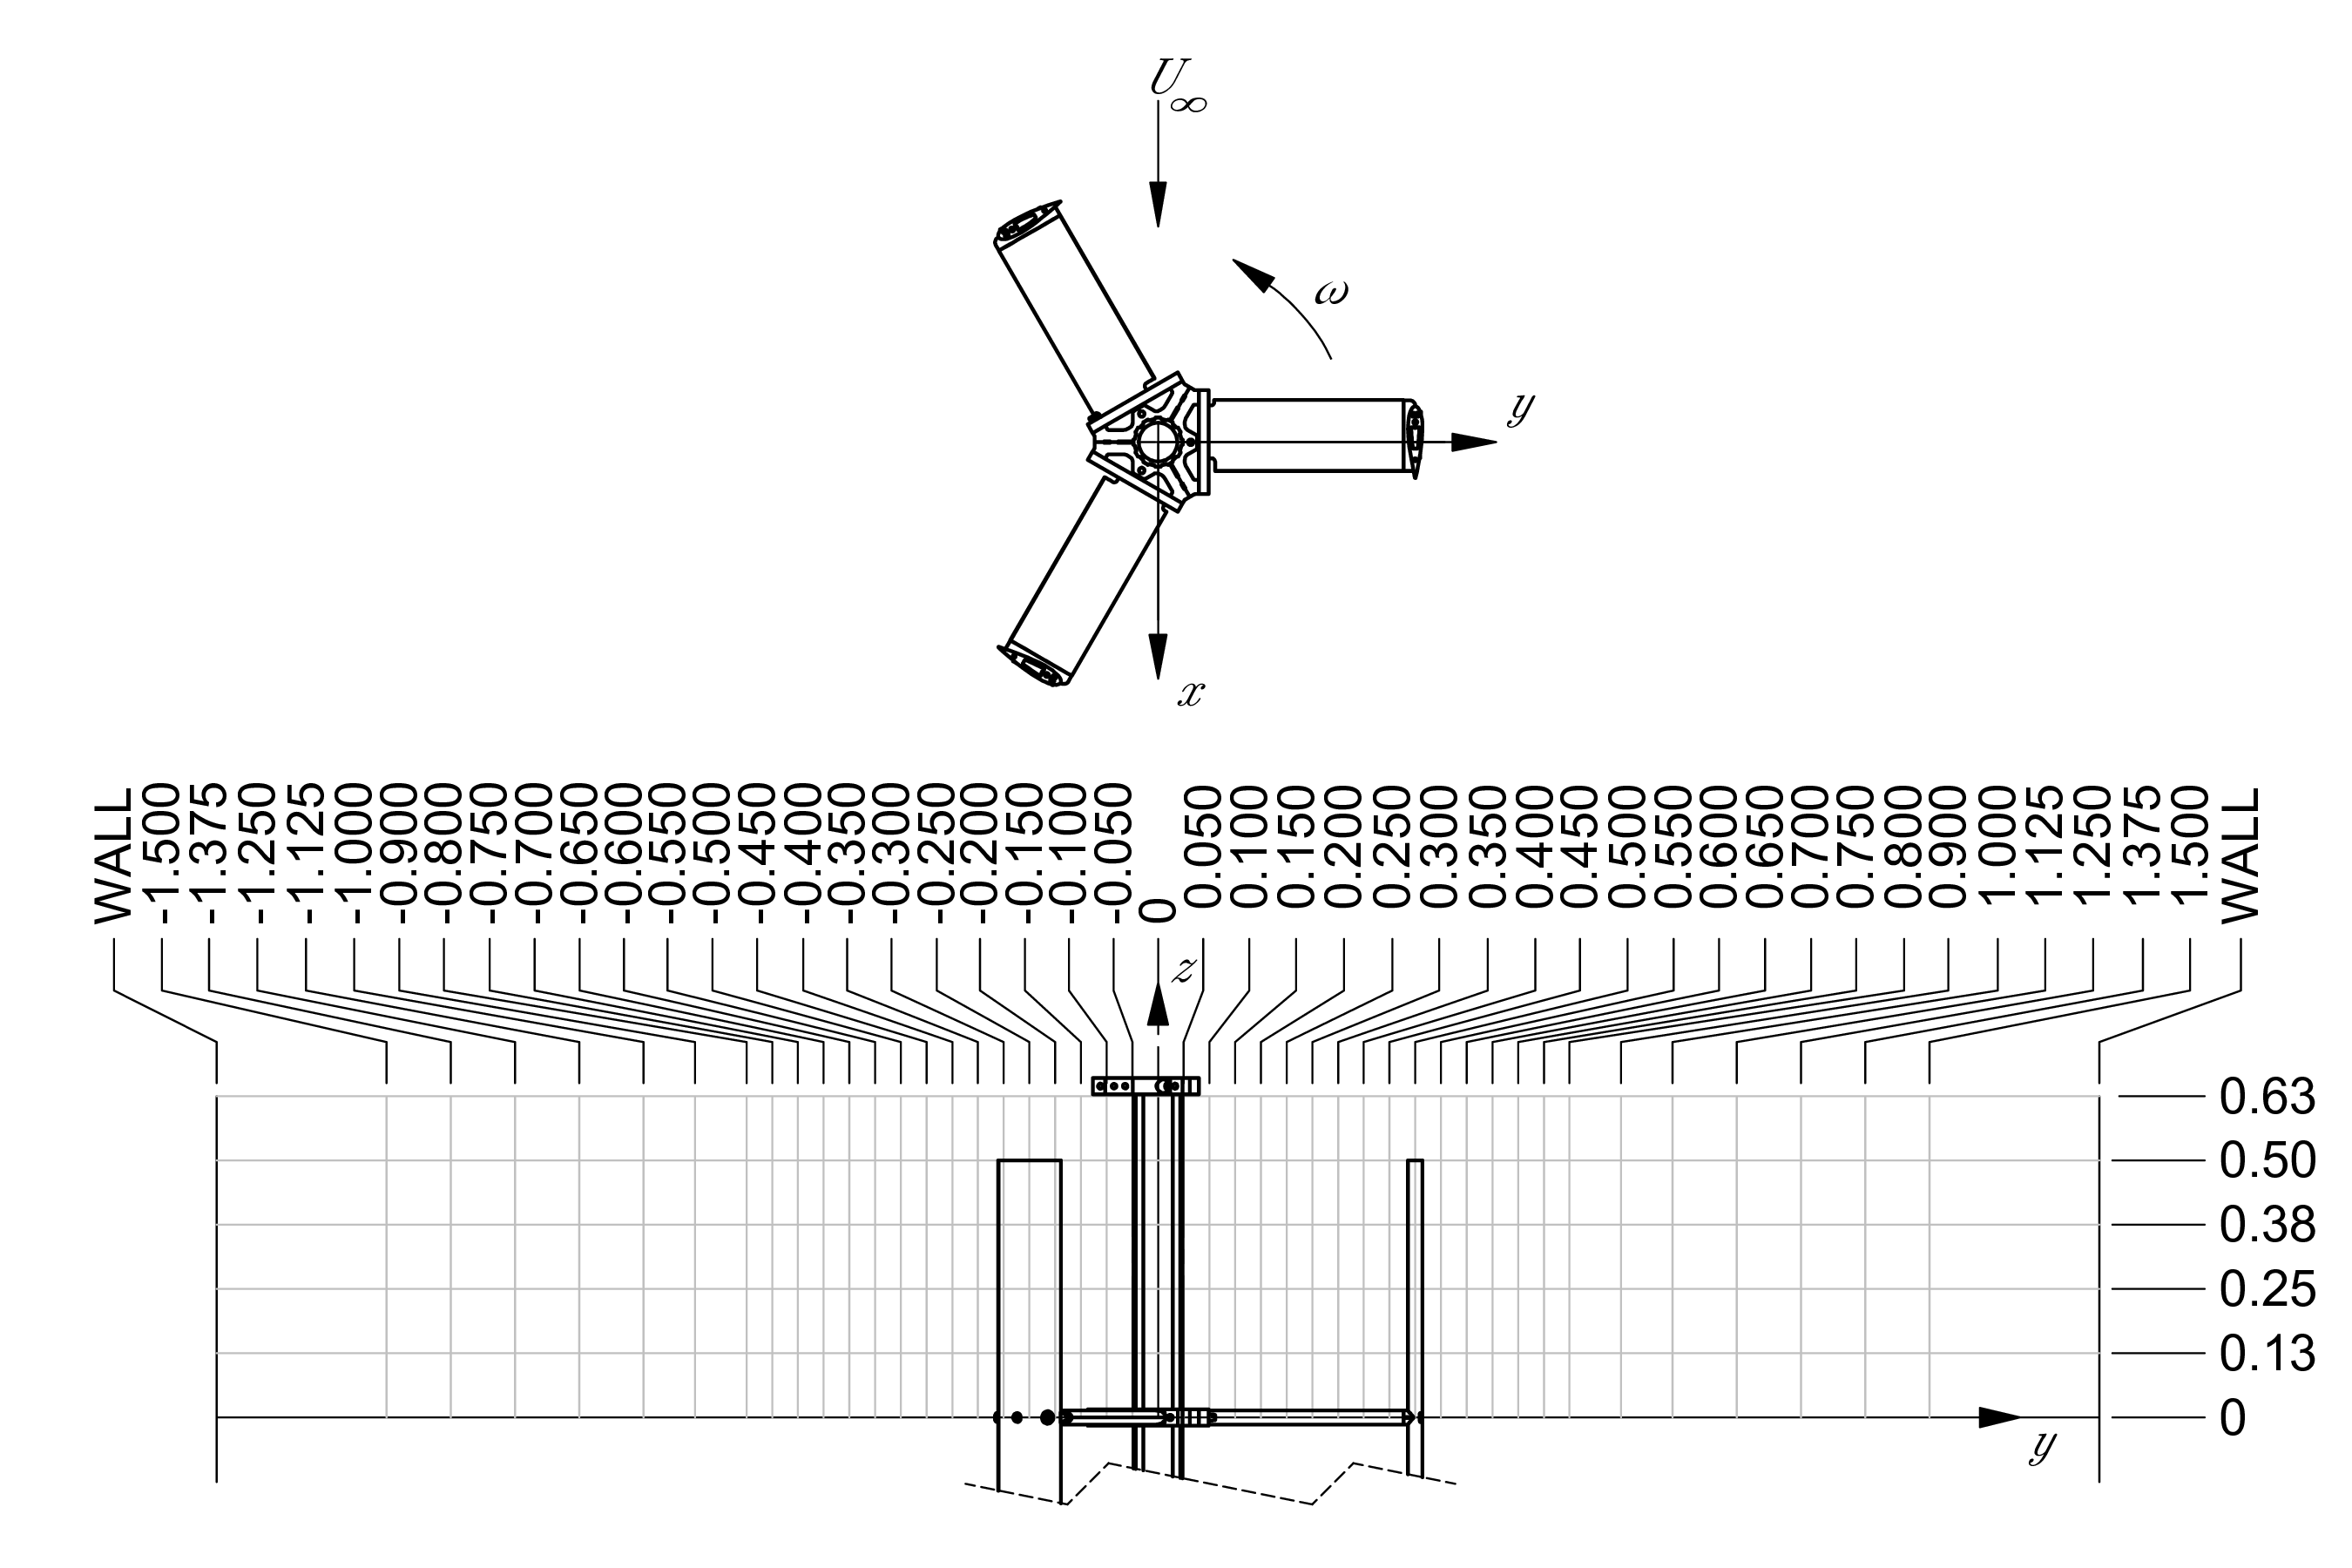
\includegraphics[width=0.99\textwidth]{unh-rvat-coord-sys}
    
    \caption{Wake measurement coordinate system and grid.}
    
    \label{fig:RVAT-baseline-wake-coordinates}
\end{figure}

For the power and drag measurements, the ADV was placed at the quarter height
$z/H = 0.25$, with $z/H=0$ corresponding to the turbine center. A duplicate set
of measurements were also taken for $z/H = 0$ to show how quarter height and
center line measurements differ as a function of tip speed ratio. One additional
transverse wake profile was then acquired at $z/H = 0.25$ for a
lower-than-optimal tip speed ratio to increase the effects of dynamic stall.


\section{Results and discussion}

\subsection{Data processing}

Data from each tow were extracted where the quantities of interest---torque,
drag, and velocity---had reached an approximately stationary mean value. The
time series were then trimmed further such that they correspond to an integer
number of turbine blade passages, to minimize bias from periodicity. Wake data
collection runs included 30 blade passages, which corresponds to approximately
16.5 seconds or 3300 velocity samples at each measuring station. Drag from the
mounting structure, a.k.a. tare drag, was measured by towing with the turbine
removed, and then subtracted from the turbine measurements to provide a better
estimate of the overall drag on the turbine rotor and shaft alone. Similarly,
tare torque was measured by driving the turbine support shaft and bearings in
air and regressing these values linearly with respect to shaft angular velocity.
This tare torque was then added to the measured turbine torque in
post-processing to provide a more accurate estimate for the true hydrodynamic
torque.

As described in Chapter~\ref{chap:exp-setup}, the tank was seeded with 11 $\mu$m
mean diameter hollow glass spheres to achieve adequate beam correlation and
signal-to-noise ratios. No filtering was used on the velocity data, i.e.,
statistics were computed using all raw samples from the measurement interval.
For computing partial derivatives of velocity quantities, a central difference
scheme was employed. For the boundaries of the measurement plane, an
inward-facing second-order scheme was used. The data processing and plotting
code, along with the reduced dataset are available from
\cite{Bachant2014-RVAT-baseline}.


\subsection{Turbine performance}

Performance curves showing the overall power and drag coefficients of the
turbine are shown in Figure~\ref{fig:RVAT-baseline-perf}. The drag coefficient
monotonically increases with increasing tip speed ratio over the entire range
tested, and the power coefficient reaches a maximum of 26\% around a tip speed
ratio $\lambda=1.8$--$1.9$, where the drag coefficient is 0.96. These curves
informed the selection of the optimal tip speed ratio $\lambda_0 = 1.9$ as the
operating point for detailed near-wake characterization. We expect that at this
tip speed ratio the turbine blades will be operating in dynamic stall over a
part of the turbine rotation \cite{Scheurich2011}, reaching maximum angles of
attack of approximately 35 degrees, and that this will be a significant
contributor to the near-wake structure. Note that the maximum power coefficient
could likely be improved with simple geometric modifications, e.g., changing the
blade pitch \cite{Fiedler2009}, but for this study the geometry was meant to be
as simple as possible, therefore the blade pitch was left at zero.

\begin{figure}
    \centering
    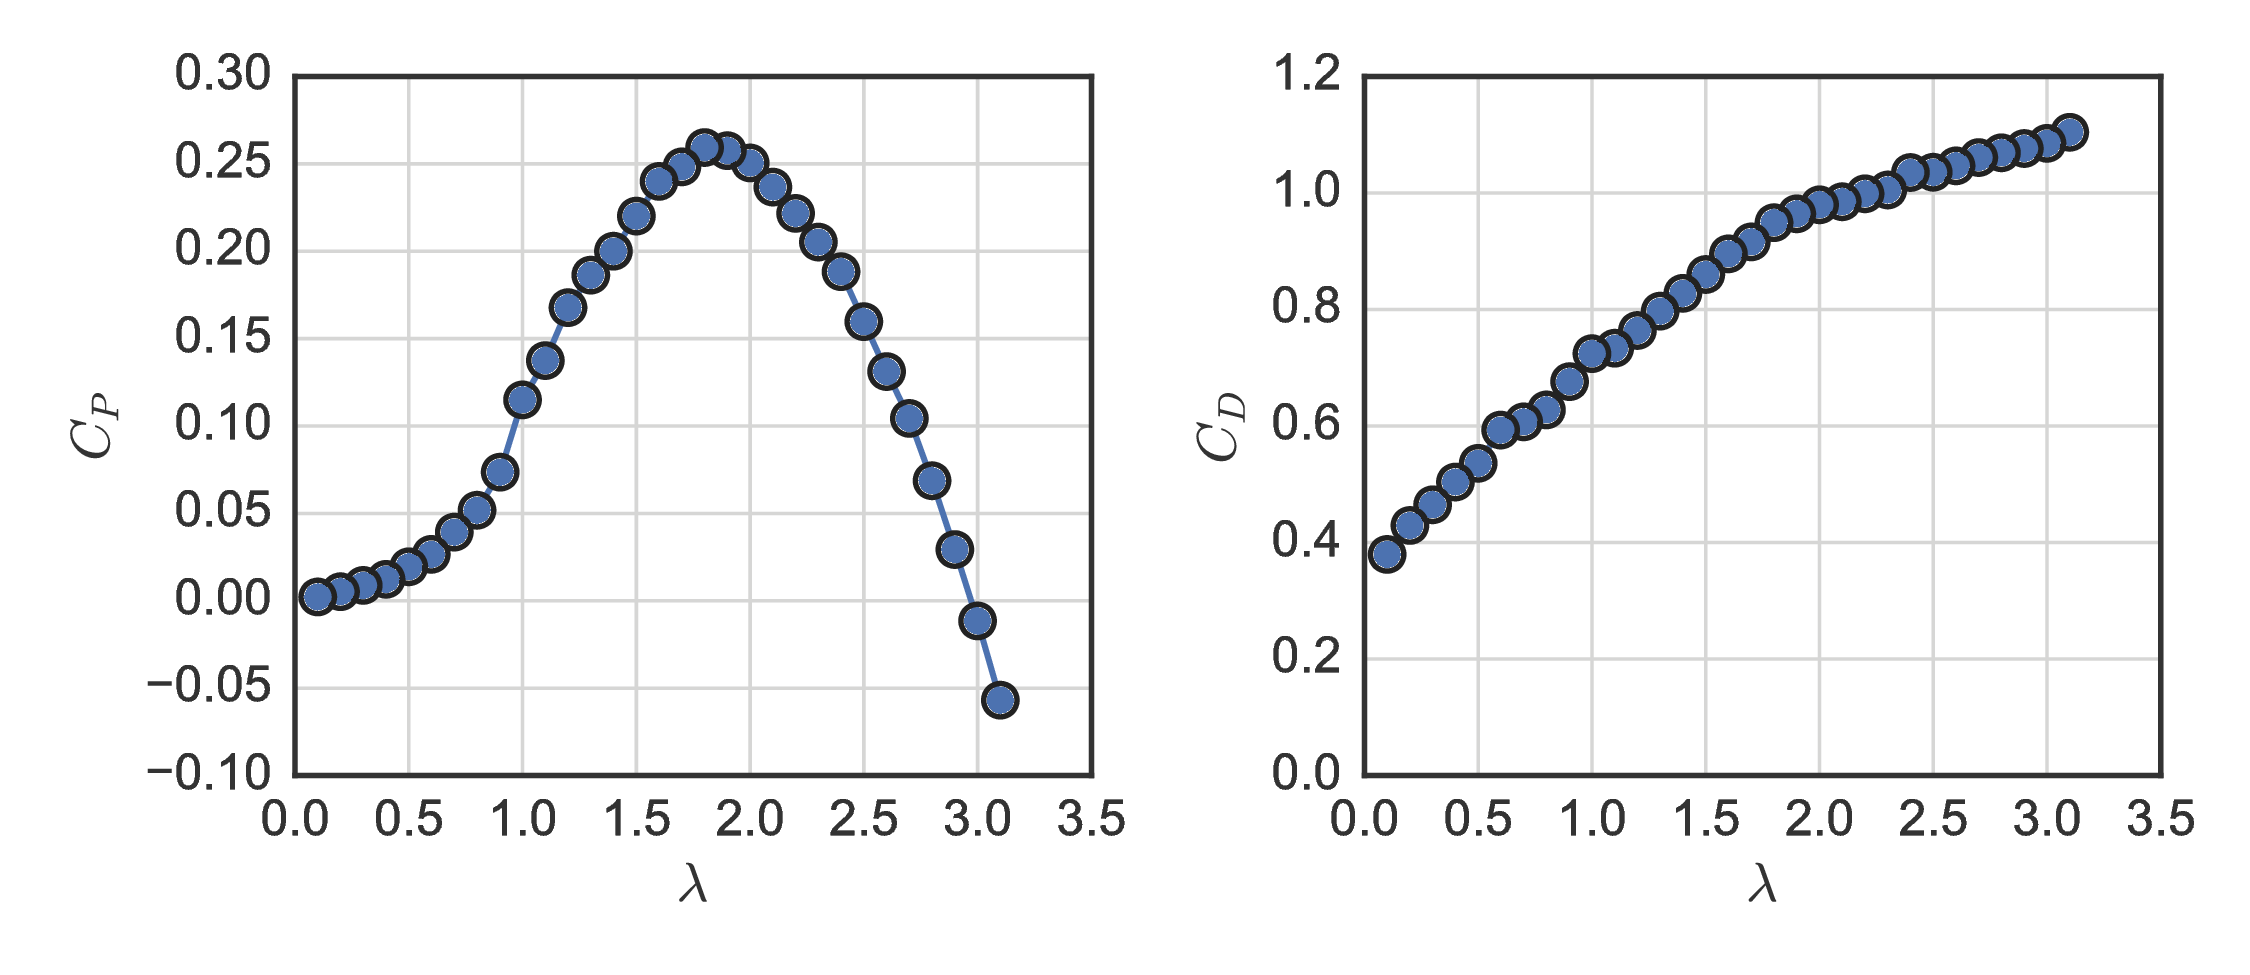
\includegraphics[width=0.9\textwidth]{RVAT-baseline_perf}
    \caption{Mean turbine power (left) and drag (right) coefficients plotted
        versus tip speed ratio.}
    \label{fig:RVAT-baseline-perf}
\end{figure}


\subsection{Wake characteristics}

The near-wake of the turbine was described in terms of its mean velocity,
streamwise vorticity, Reynolds stresses, and turbulence kinetic energy. Dominant
time scales were identified and evaluated for their contribution to the turbulent
spectra. Finally, the processes that lead to replenishment of momentum and
energy in the wake were investigated, with the goal of explaining the CFT's
relatively fast wake recovery.


\subsubsection{Momentum and vorticity}

The mean velocity measured in the wake at one turbine diameter downstream is
shown in Figure~\ref{fig:RVAT-baseline-meancontquiv}. The most obvious
characteristics are the asymmetry and three-dimensionality of the flow field.
The peak momentum deficit is shifted towards the right side of the turbine
(looking upstream). We can also see the effects of blade tip vortex shedding,
where flow is moving downward and to the left, creating strong streamwise mean
vorticity near the blade tip at $y/R=-1$, contours for which are shown in
Figure~\ref{fig:RVAT-baseline-xvorticity}. The asymmetry may explain
observations of counter-rotating turbine pairs helping speed wake recovery
\cite{Dabiri2011}.

\begin{figure}
    \centering
    
    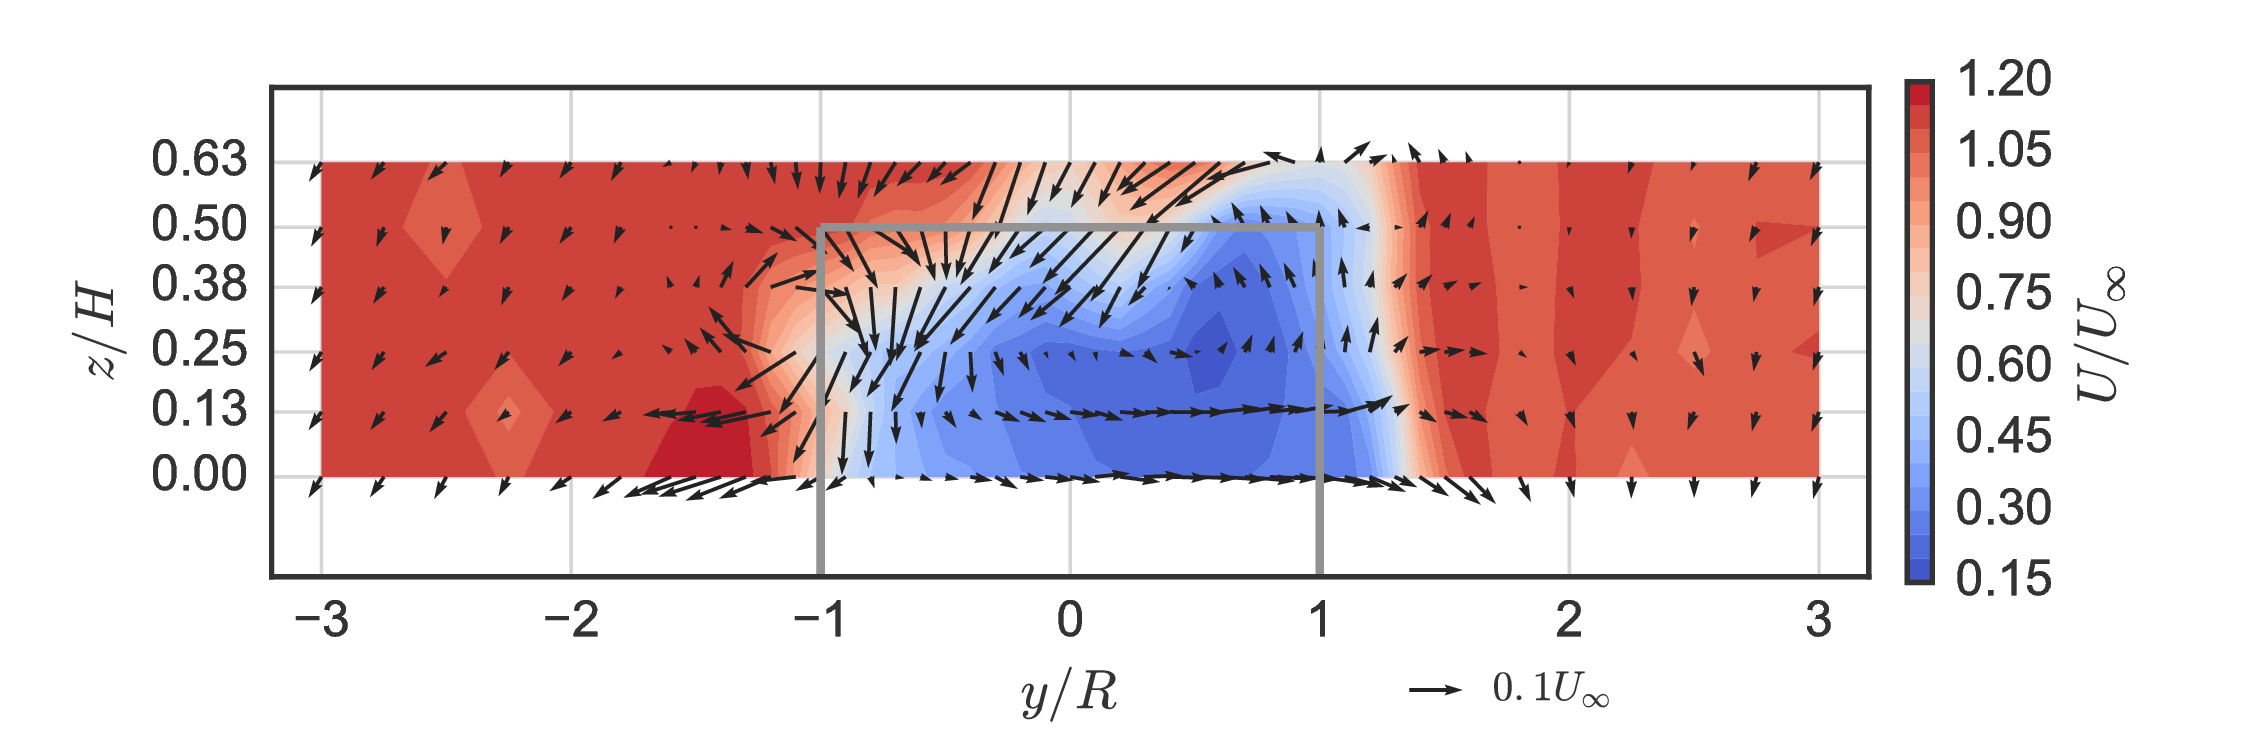
\includegraphics[width=0.9\textwidth]{RVAT-baseline_meancontquiv}
    
    \caption{Mean velocity at $\lambda=1.9$. Vectors are cross-stream and
        vertical velocities; contours are streamwise velocity. View is looking
        upstream, with the turbine frontal area indicated by the solid gray lines.}
    
    \label{fig:RVAT-baseline-meancontquiv}
\end{figure}

The generation of streamwise vorticity with opposing directions highlights once
again the three-dimensionality of the wake of this turbine, and its difference
from an axisymmetric swirling wake such as that of an axial-flow turbine. The
two regions of counter-rotating vorticity act like an asymmetrical doublet,
propelling fluid downward towards the turbine centerline.

Compared with the rotating cylinder wake measurements of Lam~\cite{Lam2009}, we
see a similar asymmetry in the mean streamwise velocity. The wake is less
asymmetrical with respect to the wake centerline for the turbine compared to the
rotating cylinder for the same non-dimensional rotation rate, although some of
these differences may be due to the cylinder experiments' lower Reynolds
numbers. Compared with the end effects of a finite cylinder
wake~\cite{Sumner2004}, we do see generation of a counter-rotating vortex pair,
though for a non-rotating cylinder these are symmetric, which is not the case
for the turbine wake, where the vortex pair seems to be tilted. The turbine's
wake is also similar to a finite cylinder wake in a sense that there is a mean
downward velocity directly behind the wake generator. These similarities and
differences give some perspective regarding the use of cylinders for turbine
simulators in physical model studies of arrays, which was considered
by~\cite{Pierce2013}.

Compared with an axial-flow turbine wake~\cite{Cal2010}, and a rotating actuator
disk model~\cite{Wu2011}, axisymmetric streamwise vorticity or swirl is not
observed here, which is one of the reasons for the wakes' differing dynamics.
This can be explained as a consequence of the conservation of angular momentum,
where the AFT imparts a streamwise rotation along its axis due to torque
generation, where the CFT imparts a torque that is perpendicular to the flow.
The AFT mean swirl only propels fluid away from its axis, while the CFT induces
mean flow into its momentum deficit region, albeit in a asymmetric fashion.

\begin{figure}
    \centering
    
    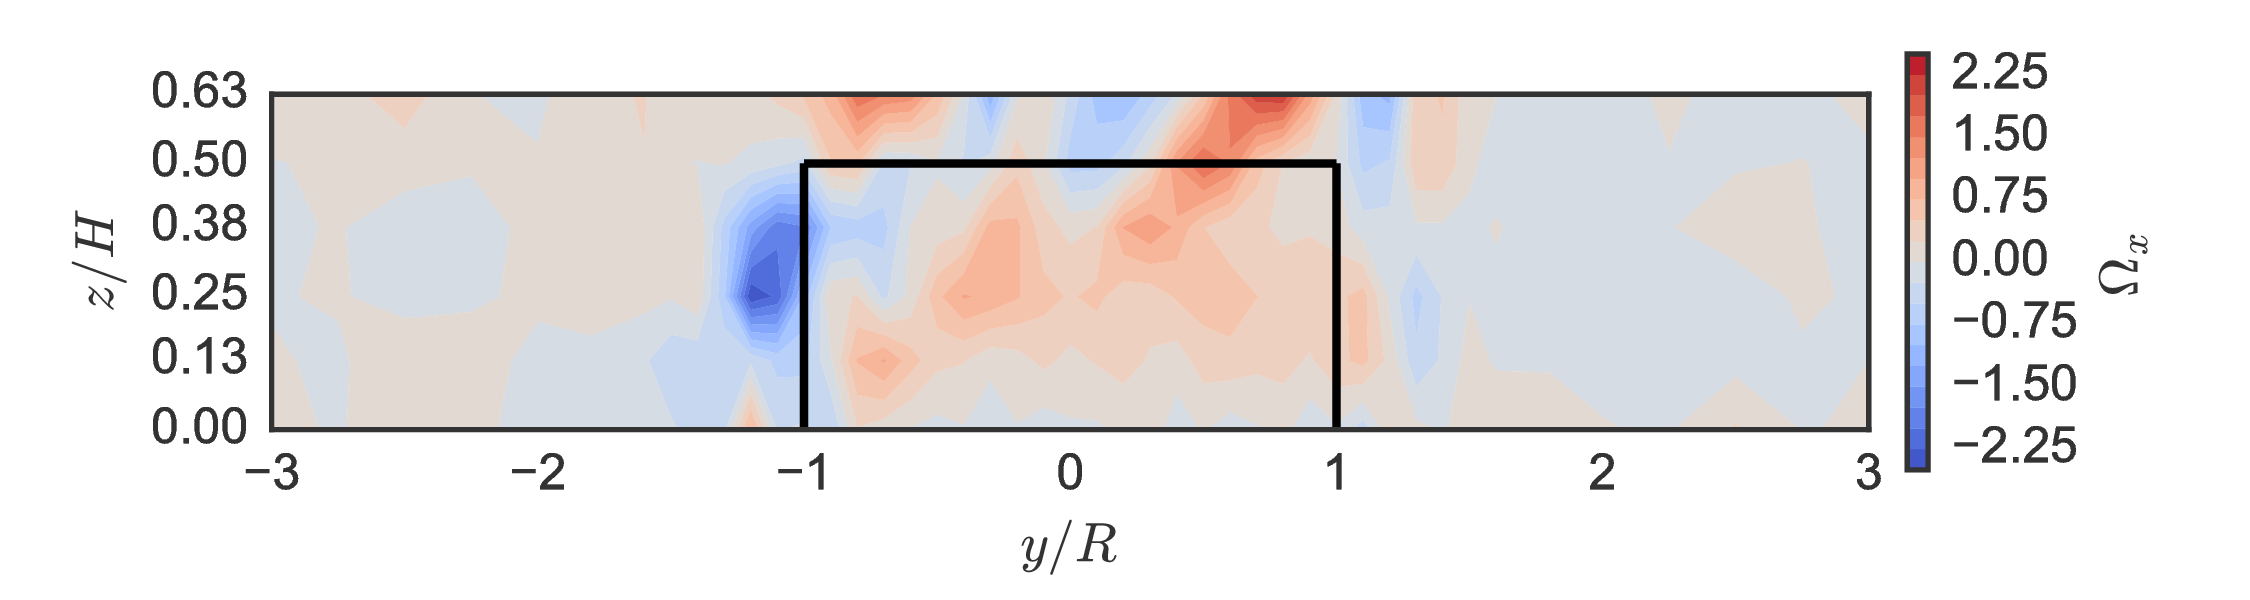
\includegraphics[width=0.9\textwidth]{RVAT-baseline_xvorticitycont}

    \caption{Contours of mean streamwise vorticity. Note that this perspective
        is looking upstream and therefore negative values indicate clockwise
        rotation.}
    
    \label{fig:RVAT-baseline-xvorticity}
\end{figure}

Reynolds shear stress contours, shown in Figure~\ref{fig:Re-stress}, quantify the
replenishment of mean momentum by turbulent transport. Regions of high
$\overline{u'v'}$ as well as the observed asymmetry correspond to the regions of
high gradients of streamwise velocity, indicating regions of high turbulence
production.


\begin{figure}
    \centering

    \begin{subfigure}{\textwidth}
        \centering
        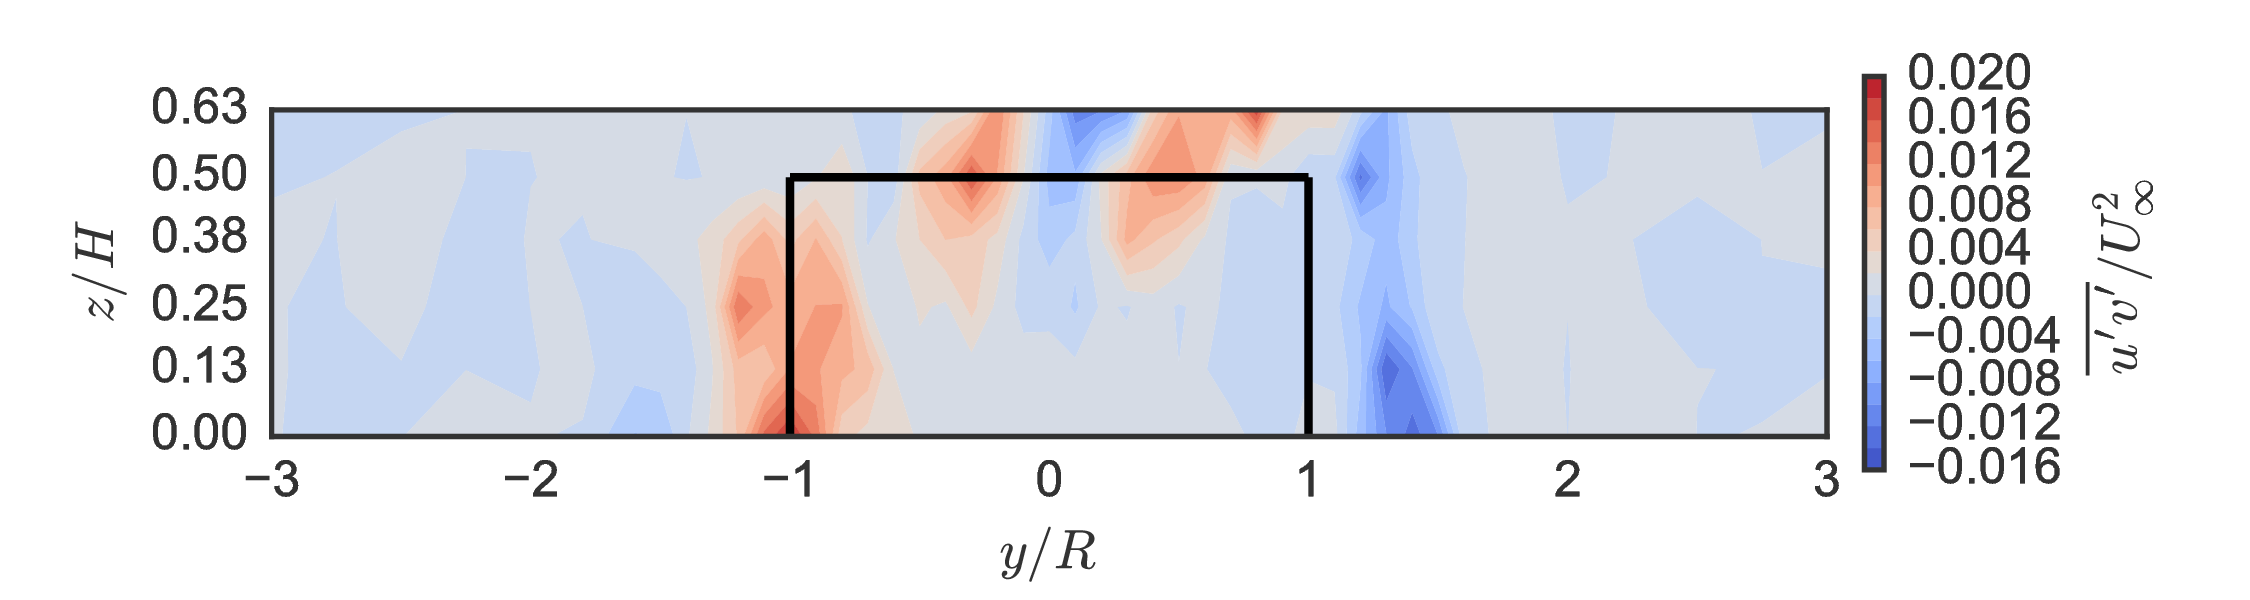
\includegraphics[width=0.8\textwidth]{RVAT-baseline_meanupvpcont}
        \caption{}
        \label{fig:RVAT-baseline-uvcont}
    \end{subfigure}
    
    \begin{subfigure}{\textwidth}
        \centering
        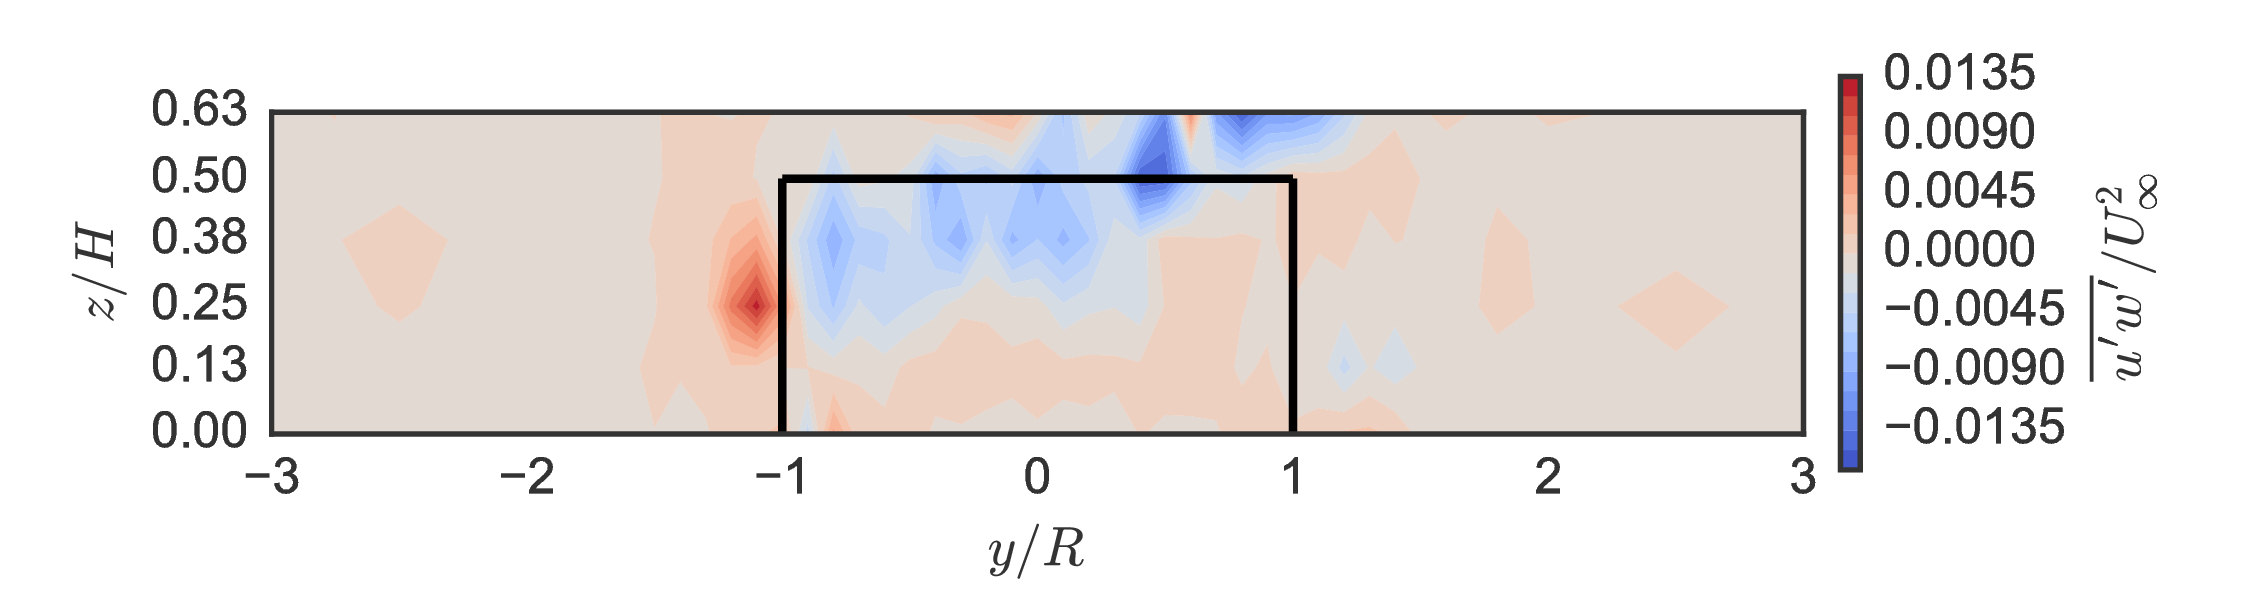
\includegraphics[width=0.8\textwidth]{RVAT-baseline_meanupwpcont}
        \caption{}
        \label{fig:RVAT-baseline-uwcont}
    \end{subfigure}
    
    \caption{Contours of (a) streamwise--cross-stream and (b)
        streamwise--vertical Reynolds shear stress.}
    
    \label{fig:Re-stress}
\end{figure}

To quantify the relative importance of mean and turbulent transport processes,
we rearrange the streamwise Reynolds-averaged momentum equation to isolate terms
contributing to its streamwise derivative. Assuming the flow is stationary in
the mean and incompressible, the equation becomes

\begin{equation}
    \begin{split}
        \frac{\p U}{\p x}  =  
        \frac{1}{U} \bigg{[}
        & - V\frac{\p U}{\p y}
        - W\frac{\p U}{\p z} \\
        & -\frac{1}{\rho}\frac{\p P}{\p x} \\
        & - \frac{\p}{\p x} \overline{u'u'}
        - \frac{\p}{\p y} \overline{u'v'}
        - \frac{\p}{\p z} \overline{u'w'} \\
        & + \nu\left(\frac{\p^2 U}{\p x^2}
        + \frac{\p^2 U}{\p y^2}
        + \frac{\p^2 U}{\p z^2} \right)
        \bigg{]}.
    \end{split}
\label{eq:momentum}
\end{equation}

From the experimental measurements, all of the terms on the right hand side were
computed except for the streamwise pressure gradient and the streamwise ($x$)
derivatives of the Reynolds and viscous stresses; the latter two terms are
expected to be small under a thin shear layer assumption. Totals for all these
terms, normalized by $D/U_\infty$ to assess nondimensional mean momentum
recovery per turbine diameter of downstream distance are plotted in
Figure~\ref{fig:mombargraph}. We see that as expected, viscous diffusion is
almost negligible. The two Reynolds stress transport terms are both significant,
but the vertical advection term dominates, and the horizontal advection term
contributes negatively, corresponding to streamlines diverging around the
turbine. The flow essentially behaves like an inviscid three-dimensional,
non-axisymmetric turbulent wake. If we sum all the terms we obtain a total wake
recovery rate at $x/D=1$ of 12\% per turbine diameter, which would be
interesting to compare with an axial-flow turbine in similar conditions.

\begin{figure}
    \centering
    
    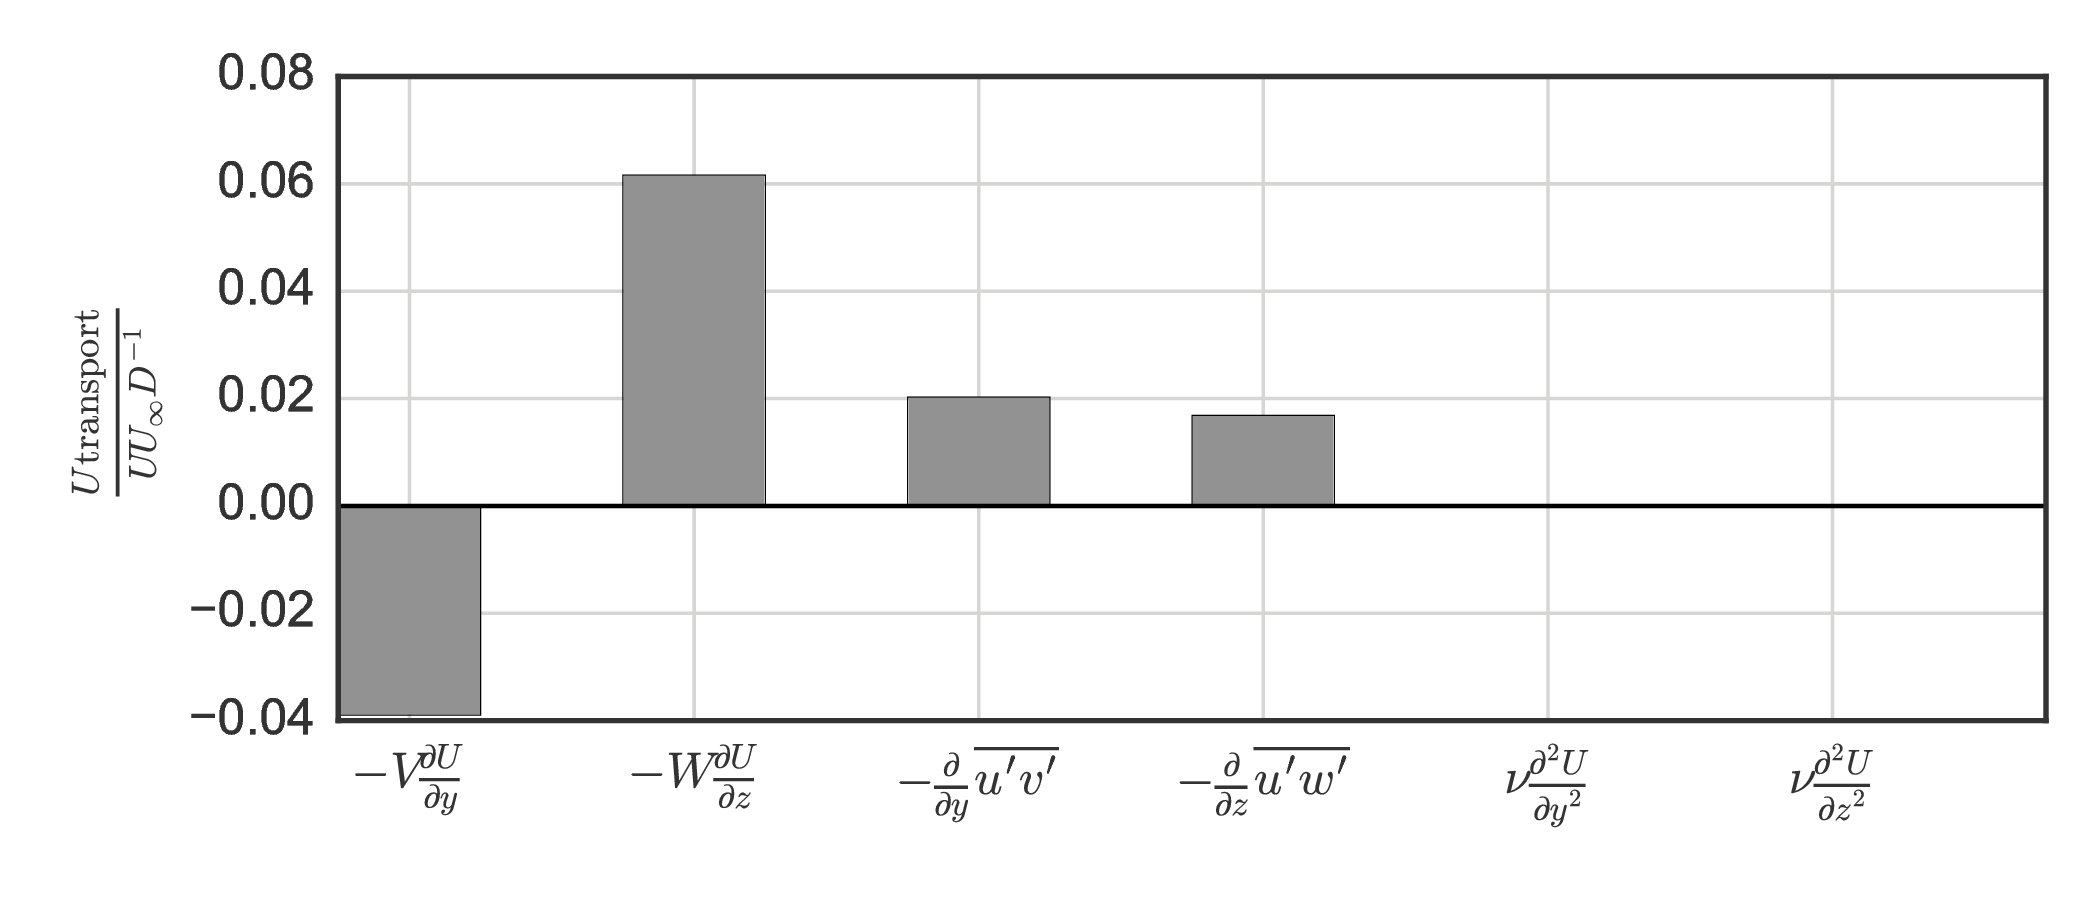
\includegraphics[width=0.9\textwidth]{RVAT-baseline_mombargraph}
    
    \caption{Estimates for the contributions to mean streamwise momentum
        recovery in the streamwise direction, multiplied by two (due to assumed
        symmetry), averaged over the measurement plane, and normalized by the
        average streamwise velocity, freestream velocity, and turbine diameter.}
    
    \label{fig:mombargraph}
\end{figure}


\subsubsection{Dominant time scales}

Spectral densities were computed using a fast Fourier transform (FFT) based
algorithm, with a Hanning window applied to the time series. Spectral values
were averaged over 4 adjacent frequencies to reduce noise and increase
confidence intervals. Figure~\ref{fig:RVAT-baseline-fpeak} shows the peak
frequency---normalized by the turbine angular frequency---of the cross-stream
velocity energy spectra at each measurement point. We can see how unsteadiness
in the flow is induced primarily at the blade passage frequency, or three times
$f_\mathrm{turbine}$. Note that some higher peak frequencies can also be seen in
this plot, out in regions of low turbulence intensity. This is due to both the
noise floor of the ADV and the wakes of the guy wire supports.

Spectral concentration $\Psi$ is quantified by normalizing the peak value of the
spectral density by the total variance of the signal multiplied by the
spectrum's Fourier frequency interval $\Delta f$, i.e.,
\begin{equation}
    \Psi \equiv \frac{S_{\max} \Delta f}{\sigma^2},
    \label{eq-spec_cont}
\end{equation}
where $\Delta f \equiv 1/(N \Delta t)$, $N$ is the total number of samples, and
$\Delta t$ is the sampling interval. For a pure harmonic $\Psi = 1$, indicating
all variance contained within a single frequency. This metric provides further
characterization of the turbulence in terms of its range of scales, rather than
the overall variance or turbulence intensity.

A plot of this concentration is also shown in
Figure~\ref{fig:RVAT-baseline-fstrength}, where it is evident that energy is
more concentrated towards the side of the  turbine where the blades move
upstream, likely seeing lower angles of attack, and therefore boundary layer
separation occurring further towards the trailing edge of the blade. This
concentration is indicative of more coherent motion, or extraction of
energy/momentum from the flow without intense separation, whereas on the
opposite side of the turbine, turbulence generated by the dynamic stall process
is increasing the diffusion of shed vorticity. This effect can be further
illustrated looking at sample spectra for turbine torque coefficient and
cross-stream velocity components at two points on opposite sides of the turbine,
shown in Figure~\ref{fig:RVAT-baseline-multispec}, where the cross-stream
velocity at the side of the turbine inducing massive separation shows a smaller
peak in its spectrum at the blade passage frequency.

\begin{figure}
    \centering
    
    \begin{subfigure}{\textwidth}
        \centering
        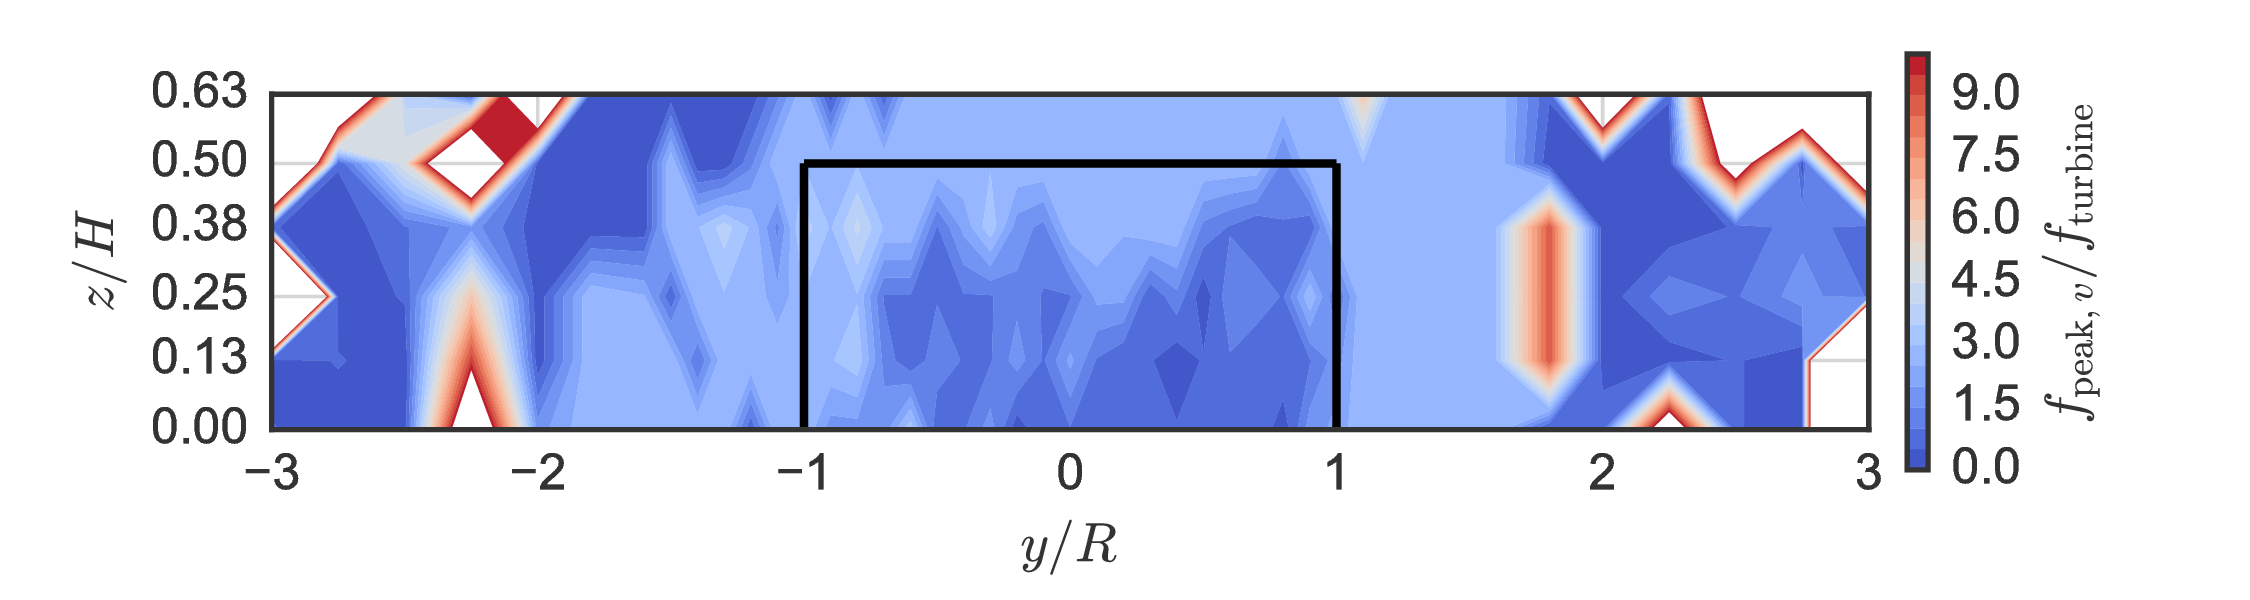
\includegraphics[width=0.9\textwidth]{RVAT-baseline_fpeak_vcont}
        \caption{}
        \label{RVAT-baseline-fpeak}
    \end{subfigure}
    
    \begin{subfigure}{\textwidth}
        \centering
        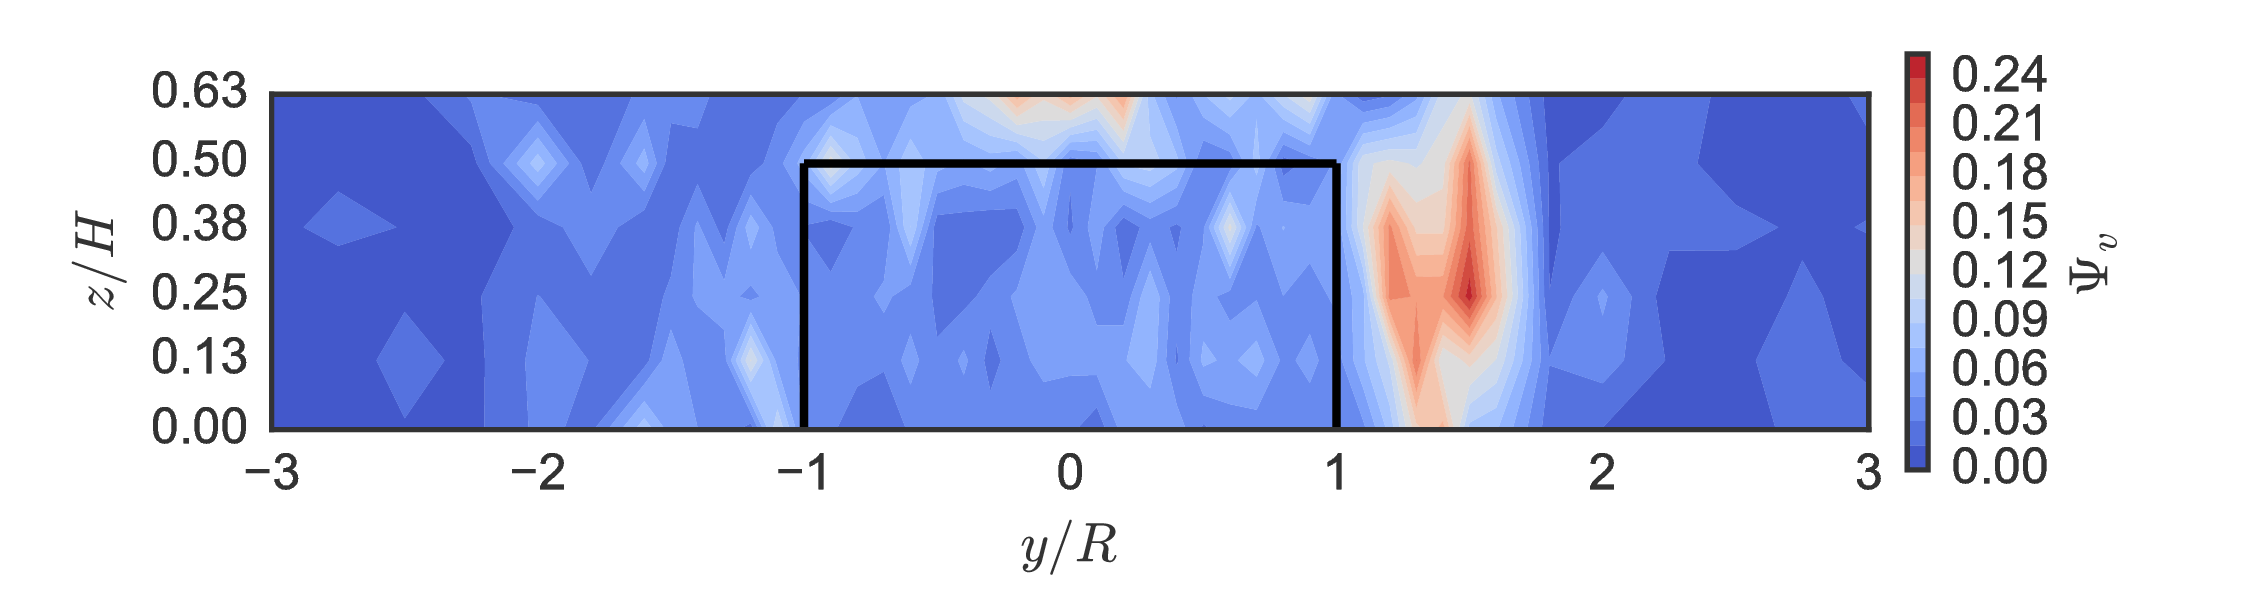
\includegraphics[width=0.9\textwidth]{RVAT-baseline_fstrength_vcont}
        \caption{}
        \label{RVAT-baseline-fstrength}
    \end{subfigure}

    \caption{Cross-stream velocity energy spectra (a) peak frequency normalized by
        turbine angular frequency and (b) spectral concentration. Note
        that white regions have values higher than the maximum value of the color
        bar, caused by both noise and wakes of the guy wire supports.}
    
    \label{fig:RVAT-baseline-fcont}
\end{figure}

\begin{figure}
    \centering

    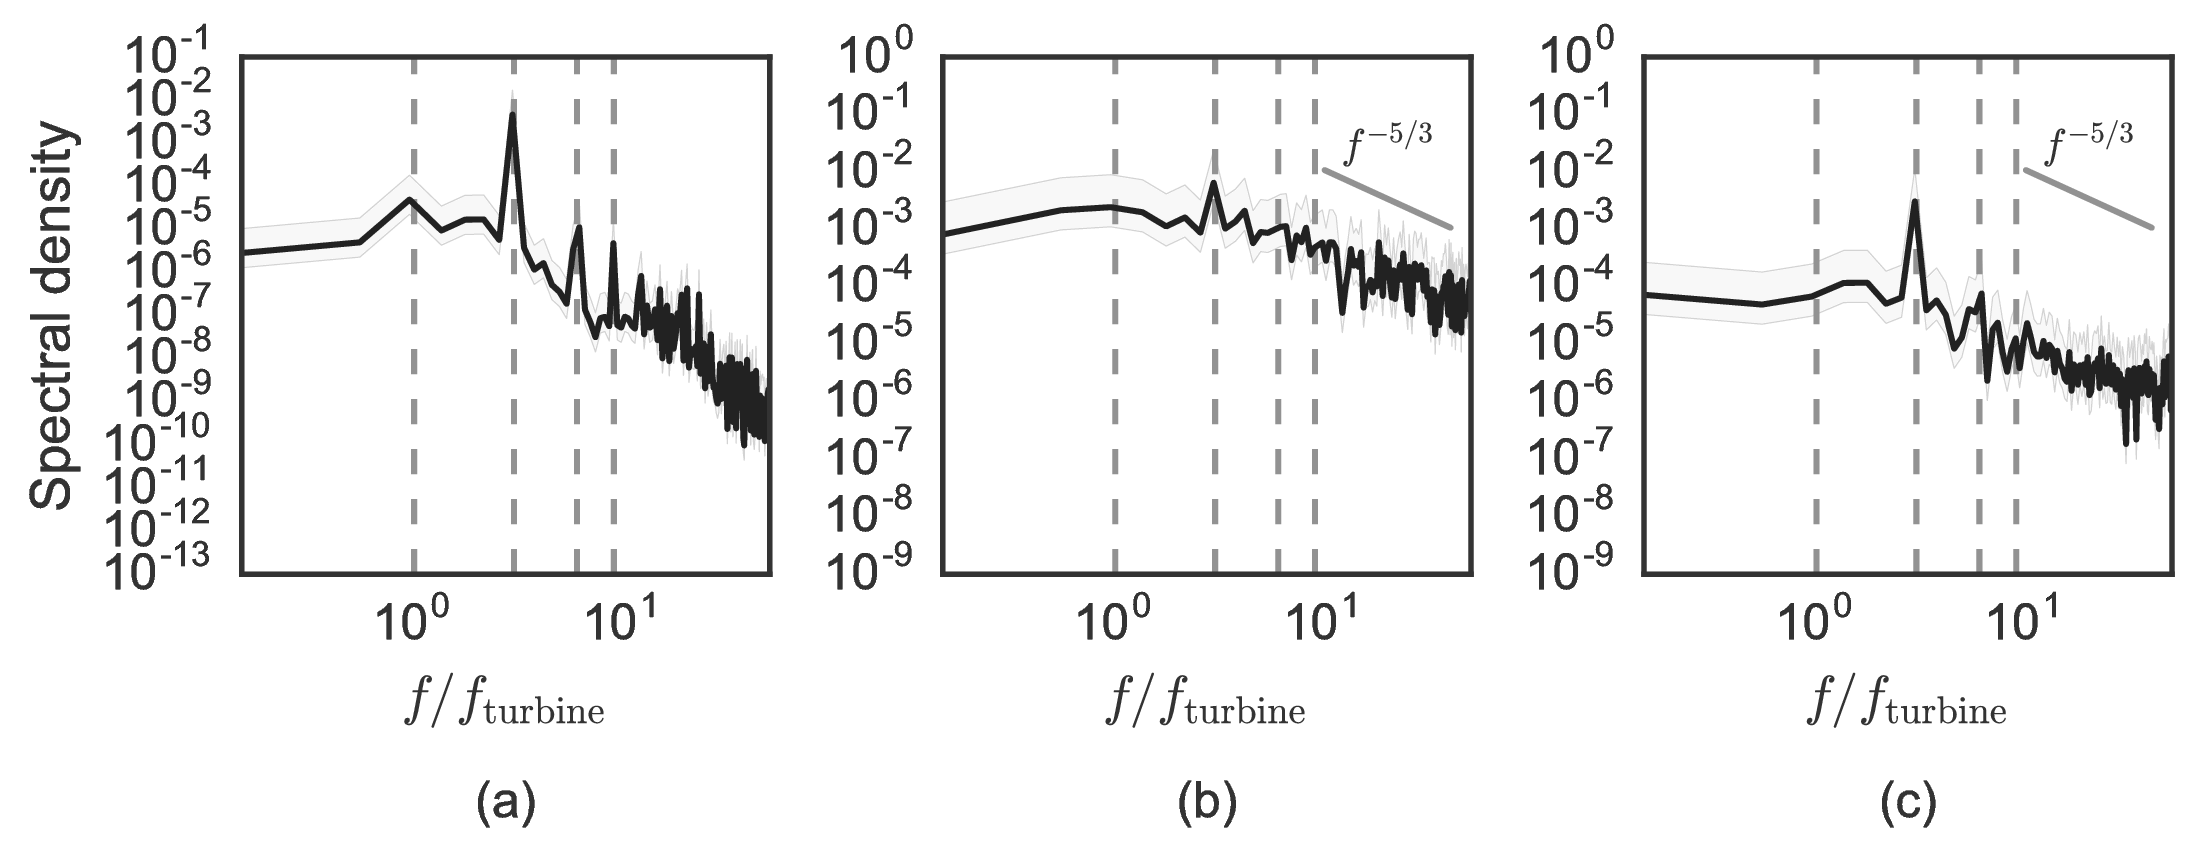
\includegraphics[width=0.95\textwidth]{RVAT-baseline_multispec}

    \caption{Spectral density for (a) torque coefficient, (b) cross-stream
        velocity at $y/R = -1$; $z/H = 0.25$, and (c) cross-stream velocity at $y/R
        = 1.5$; $z/H = 0.25$. Dashed vertical lines indicate $[1, 3, 6, 9]$ times
        the turbine rotational frequency and the shaded gray region indicates the
        95\% confidence interval for a $\chi^2$ variable with 8 degrees of
        freedom---twice the number of frequencies over which spectral values were
        averaged to reduce noise.}
    
    \label{fig:RVAT-baseline-multispec}
\end{figure}


\subsubsection{Kinetic energy}

Contours of turbulence kinetic energy are shown in
Figure~\ref{fig:RVAT-baseline-kcont}. The turbulence kinetic energy is
concentrated near the top and left side of the turbine, as a result of the blade
tip and dynamic stall vortex shedding, respectively. The lower turbulence
kinetic energy on the $+y$ side of the turbine corresponds with the more
concentrated spectral energy of velocity unsteadiness in this area. This can be
interpreted as the lift-induced vorticity being shed with less separation
compared to the $-y$ side of the turbine, where turbulence is being generated
and redistributing energy across a larger bandwidth. This brings up one
potential improvement to actuator line models: Modulating turbulence fields at
the occurrence of dynamic stall.

\begin{figure}
    \centering

    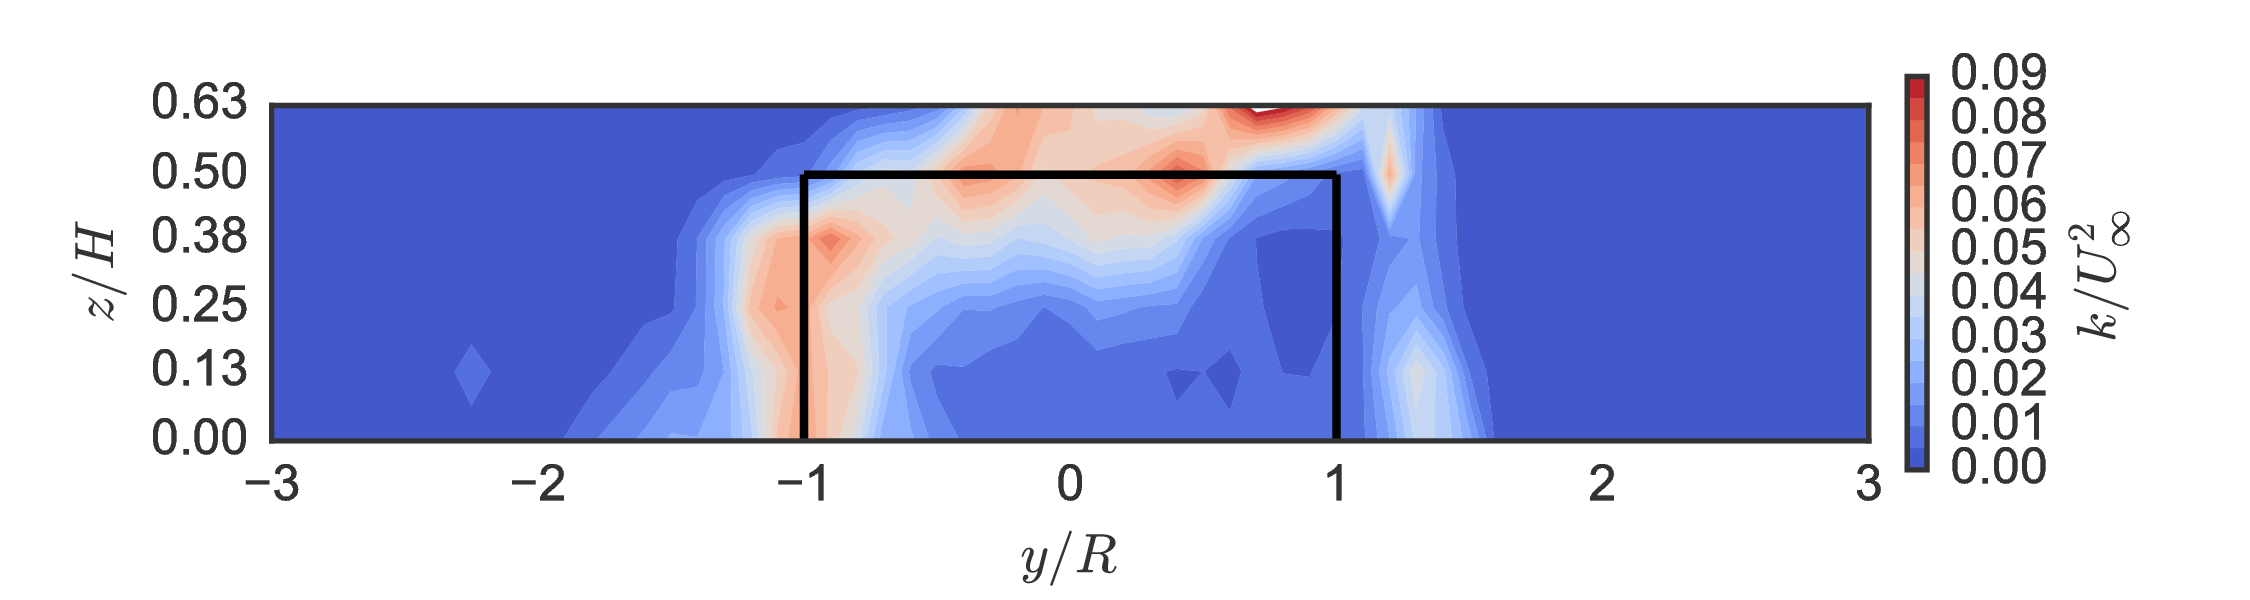
\includegraphics[width=0.9\textwidth]{RVAT-baseline_kcont}

    \caption{Contours of normalized turbulence kinetic energy. Turbine frontal
        area is indicated by solid black lines.}
    
    \label{fig:RVAT-baseline-kcont}
\end{figure}

Like the analysis of the mean streamwise momentum, the mechanisms which play the
most important role in mean kinetic energy recovery as the wake evolves in the
streamwise direction are now examined. The transport equation for the kinetic
energy $K$ associated with the mean flow \cite{TennekesAndLumley}, rearranged to
isolate the streamwise recovery can be written as
\begin{equation}
    \begin{split}
        \frac{\p K}{\p x}
        =
        \frac{1}{U}
        \bigg{[}
        & - \underbrace{V \frac{\p K}{\p y}}_{y\text{-adv.}}
        - \underbrace{W \frac{\p K}{\p z}}_{z\text{-adv.}}
        % Pressure work:
        - \frac{1}{\rho}\frac{\p}{\p x_j} P U_i \delta_{ij}
        % Work by viscous forces
        + \frac{\p}{\p x_j} 2 \nu U_i S_{ij}
        % Turbulent transport of K
        - \underbrace{
            \frac{1}{2}\frac{\p}{\p x_j} \overline{u_i' u_j'} U_i
        }_{\text{Turb. trans.}} \\
        % Production of k
        & + 
        \underbrace{
            \overline{u_i' u_j'} \frac{\p U_i}{\p x_j}
        }_{k\text{-prod.}}
        - 
        \underbrace{
            2 \nu S_{ij}S_{ij}
        }_{\text{Mean diss.}}
        \bigg{]}.
    \label{eq-K_full}
    \end{split}
\end{equation}
The terms of interest are labeled---advection in the cross-stream and vertical
directions, energy transport by turbulent fluctuations, production of turbulence
kinetic energy $k$ through mean shear, and the dissipation due to mean viscous
shear forces. For the tensor terms, streamwise derivatives were ommitted, since
the measurements were limited to a single streamwise distance.
Table~\ref{tab:RVAT-baseline-eqs} lists all components kept for the computation
of each transport term.

\begin{table}
    \centering
    \begin{tabular}{c|c}
        Term in Eq.~\ref{eq-K_full} & Implementation \\ 
        \hline  
        $y$-adv. & $-\frac{V}{U}\frac{\p K}{\p y}$ \\ 
        $z$-adv.  & $-\frac{W}{U}\frac{\p K}{\p z}$ \\ 
        Turb. trans. ($y$) & $-\frac{1}{2U} \big{[} \frac{\p }{\p y}\overline{u'v'}U 
        + \frac{\p }{\p y}\overline{v'v'}V + \frac{\p }{\p y}\overline{w'v'}W \big{]} $\\ 
        Turb. trans. ($z$)  & $-\frac{1}{2U} \big{[} \frac{\p }{\p z}\overline{u'w'}U 
        + \frac{\p }{\p z}\overline{v'w'}V + \frac{\p }{\p z}\overline{w'w'}W \big{]} $\\ 
        $k$-prod.  & $\frac{1}{U} \big{[} \overline{u'v'}\frac{\p U}{\p y}
        + \overline{v'v'}\frac{\p V}{\p y} 
        + \overline{w'v'}\frac{\p W}{\p y} $ \\
        & $ + \overline{u'w'}\frac{\p U}{\p z}
        + \overline{v'w'}\frac{\p V}{\p z}
        + \overline{w'w'}\frac{\p W}{\p z}
        \big{]} $ \\ 
        Mean diss.   & $ - \frac{2 \nu}{U} \big{[}
        \big{(} \frac{\p U}{\p y} \big{)}^2
        + \big{(} \frac{\p U}{\p z} \big{)}^2
        + \big{(} \frac{\p V}{\p y} \big{)}^2 $ \\
        & $
        + \big{(} \frac{\p V}{\p z} \big{)}^2
        + \big{(} \frac{\p W}{\p y} \big{)}^2
        + \big{(} \frac{\p W}{\p z} \big{)}^2
        \big{]} $ \\ 
    \end{tabular} 
    \caption{Terms used to compute contributions to mean kinetic energy recovery.}
    \label{tab:RVAT-baseline-eqs}
\end{table}

Figure~\ref{fig:RVAT-baseline-Kturbtrans} shows estimates of mean kinetic energy
transport by turbulent fluctuations. The structure of this plot indicates that
the turbulent fluctuations transport mean kinetic energy inward towards regions
of lower mean momentum and lower mean kinetic energy. The signs of the terms
plotted here can be understood from Figures 6 and 4. Note that despite lower
turbulence kinetic energy on the $+y$ side of the turbine, magnitudes of the
turbulent transport are similar on both.


\begin{figure}
    \centering
    
    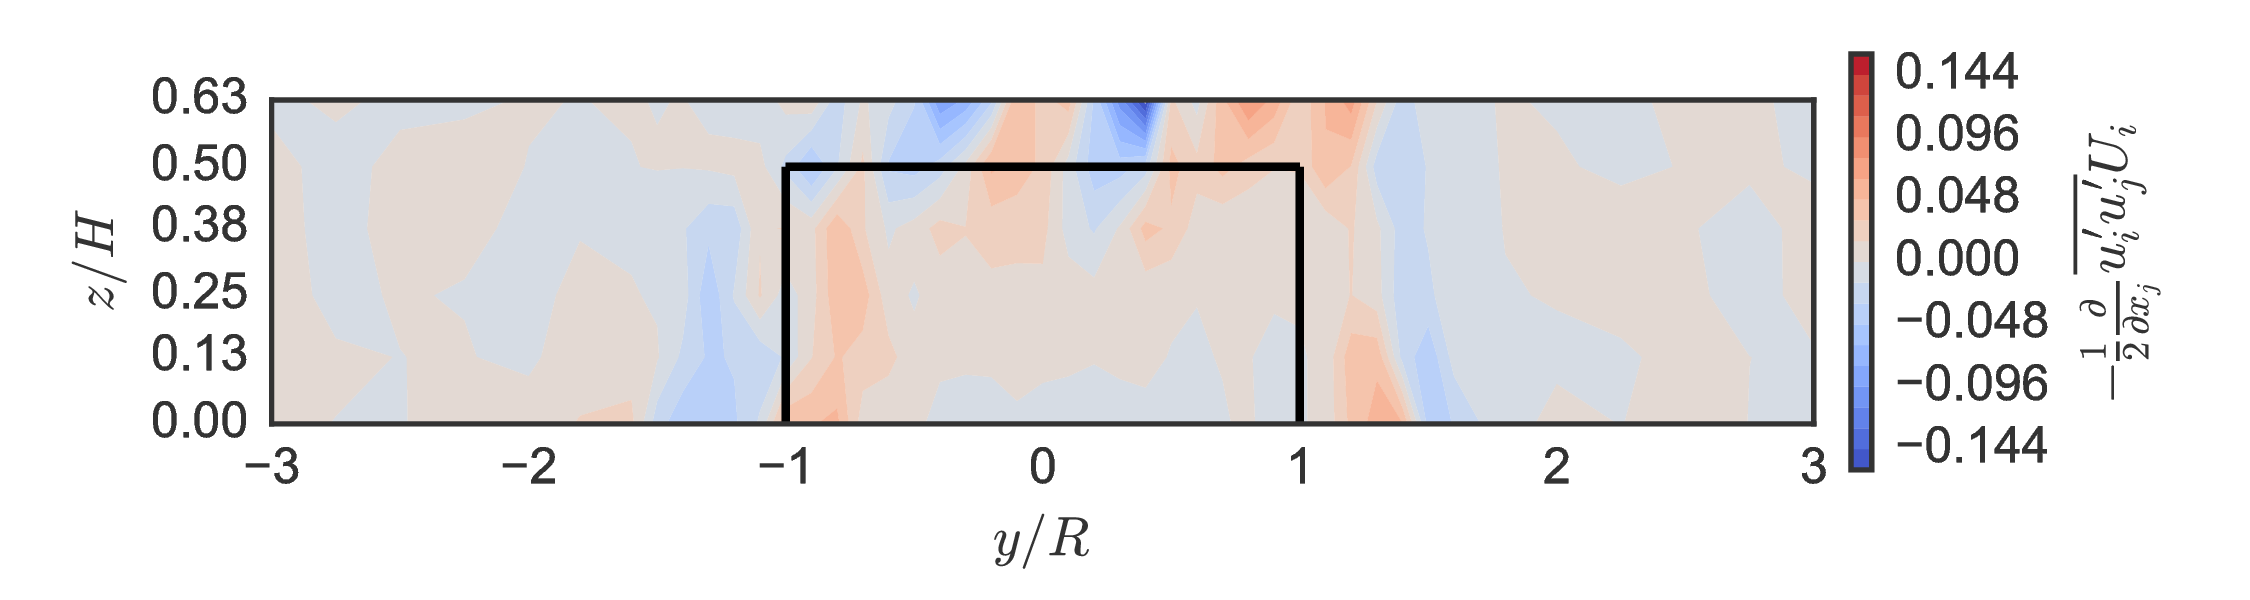
\includegraphics[width=0.9\textwidth]{RVAT-baseline_Kturbtranscont}

    \caption{Contours of estimated mean kinetic energy transport by turbulent
        fluctuations, where streamwise derivatives are omitted. Turbine frontal area
        is indicated by solid black lines.}
    
    \label{fig:RVAT-baseline-Kturbtrans}
\end{figure}

Contributions to mean kinetic energy recovery from various mechanisms were
averaged over the  measurement plane using the trapezoidal rule.
Figure~\ref{fig:RVAT-baseline-Kbargraph} shows the normalized sum of each
quantity to show their relative size. As with the momentum, the cross-stream
mean advection contributes negatively since the flow is accelerating around the
turbine due to its pressure disturbance, where streamlines diverge.

Viscous dissipation due to mean shear is essentially negligible compared to
the other terms, which is to be expected in a high Reynolds number shear flow a 
short distance downstream of the shear flow (wake) generator (CFT).

Production of turbulence kinetic energy acts to reduce mean kinetic energy, as
expected for the mean kinetic energy equation. The turbulent transport terms,
separated by the direction of their divergence, i.e., ``$y$-turb.'' is a sum of
all terms with $\p / \p y$ in them and ``$z$-turb.'' is a sum of all terms with
$\p / \p z$ in them, are about the same order of magnitude, both roughly an
order of magnitude smaller than the vertical advection term, which is the
largest. It should be re-stated that the terms in
Figure~\ref{fig:RVAT-baseline-Kbargraph} were evaluated in the near wake, in a
measurement plane at $x/D=1$ shown in
Figure~\ref{fig:RVAT-baseline-wake-coordinates}.

Compared to the observations of Kinzel \etal~\cite{Kinzel2012}, where the
turbulent transport terms were found to be not large enough to replenish turbine
power output, it can be seen here that it is most likely vertical advection that
plays the most important role in enhancing the wake recovery, not the turbulence
quantities. This is likely a consequence of the unique vorticity generation and
interaction from lift production, (dynamic) stall vortices, and blade end
effects.

\begin{figure}
    \centering
    
    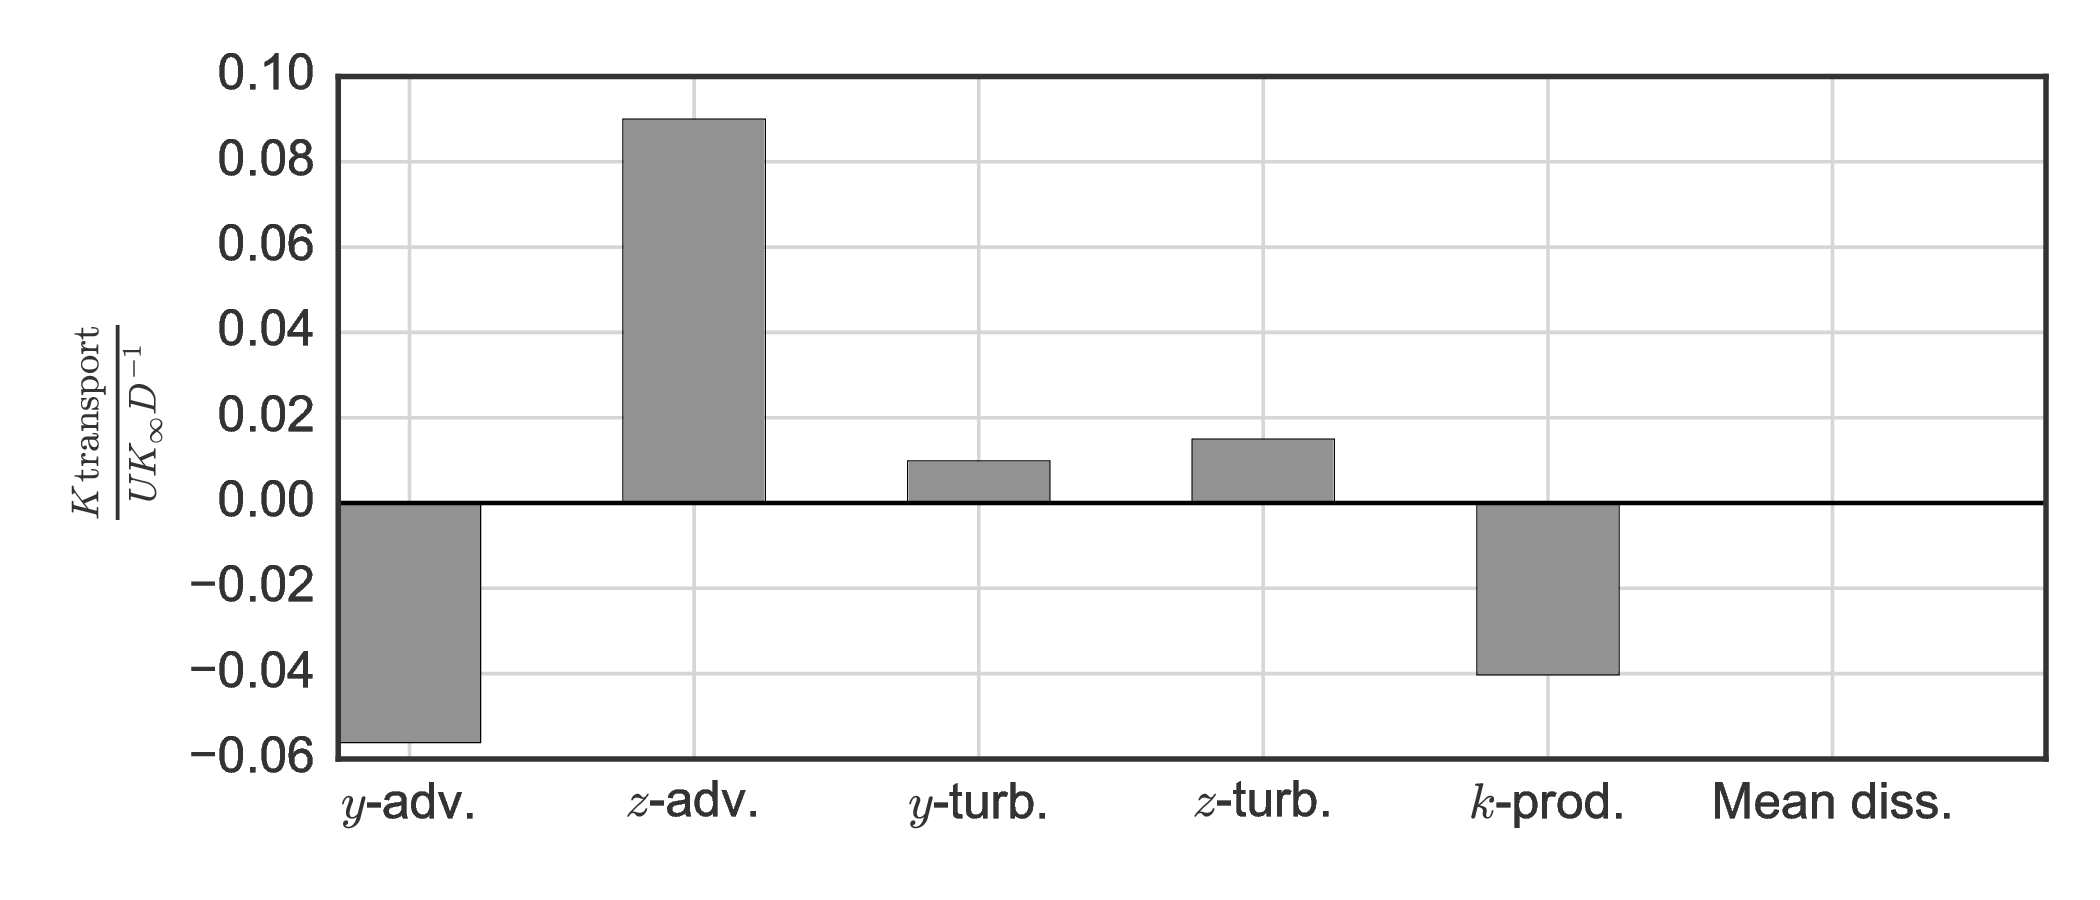
\includegraphics[width=0.9\textwidth]{RVAT-baseline_Kbargraph}

    \caption{Estimates for the contributions to mean kinetic energy recovery in
        the streamwise direction, multiplied by two (due to assumed symmetry),
        averaged over the measurement plane, and normalized by the average
        streamwise advection velocity, freestream kinetic energy, and turbine
        diameter.}
    
    \label{fig:RVAT-baseline-Kbargraph}
\end{figure}


\subsection{Effects of tip speed ratio}

Low tip speed ratio may occur temporarily during a gust inflow condition, may be
caused by malfunctioning controls, or may be the optimal operating point for a
high solidity turbine. From our measurements we can observe how mean velocities
at two fixed points downstream of the turbine axis vary with tip speed ratio.
These velocity components are plotted in
Figure~\ref{fig:RVAT-baseline-mean-vel-vs-tsr}. Mean streamwise velocity deficit
at $z/H = 0$ increases with tip speed ratio, which is expected in light of the
drag measurements. However, mean velocity deficit at the quarter height is
highest at tip speed ratios corresponding to high power coefficient, but
decreases at higher values of $\lambda$. Mean vertical velocity at the turbine
center remains relatively constant across the entire operating envelope.
However, mean vertical velocity at the quarter height shows a markedly higher
downward component at higher $\lambda$, corresponding to the similar
aforementioned trend of decreasing streamwise velocity deficit at that location.
Asymmetry about $y/R=0$ is seen in the mean cross-stream velocity at values of
$\lambda$ away from those of highest power output, with a mean component in the
positive $y$-direction. These effects may be attributed to a shift in the blade
position at which maximum loading occurs, therefore changing the strength and
orientation of the blade tip vortices.

\begin{figure}
    \centering
    
    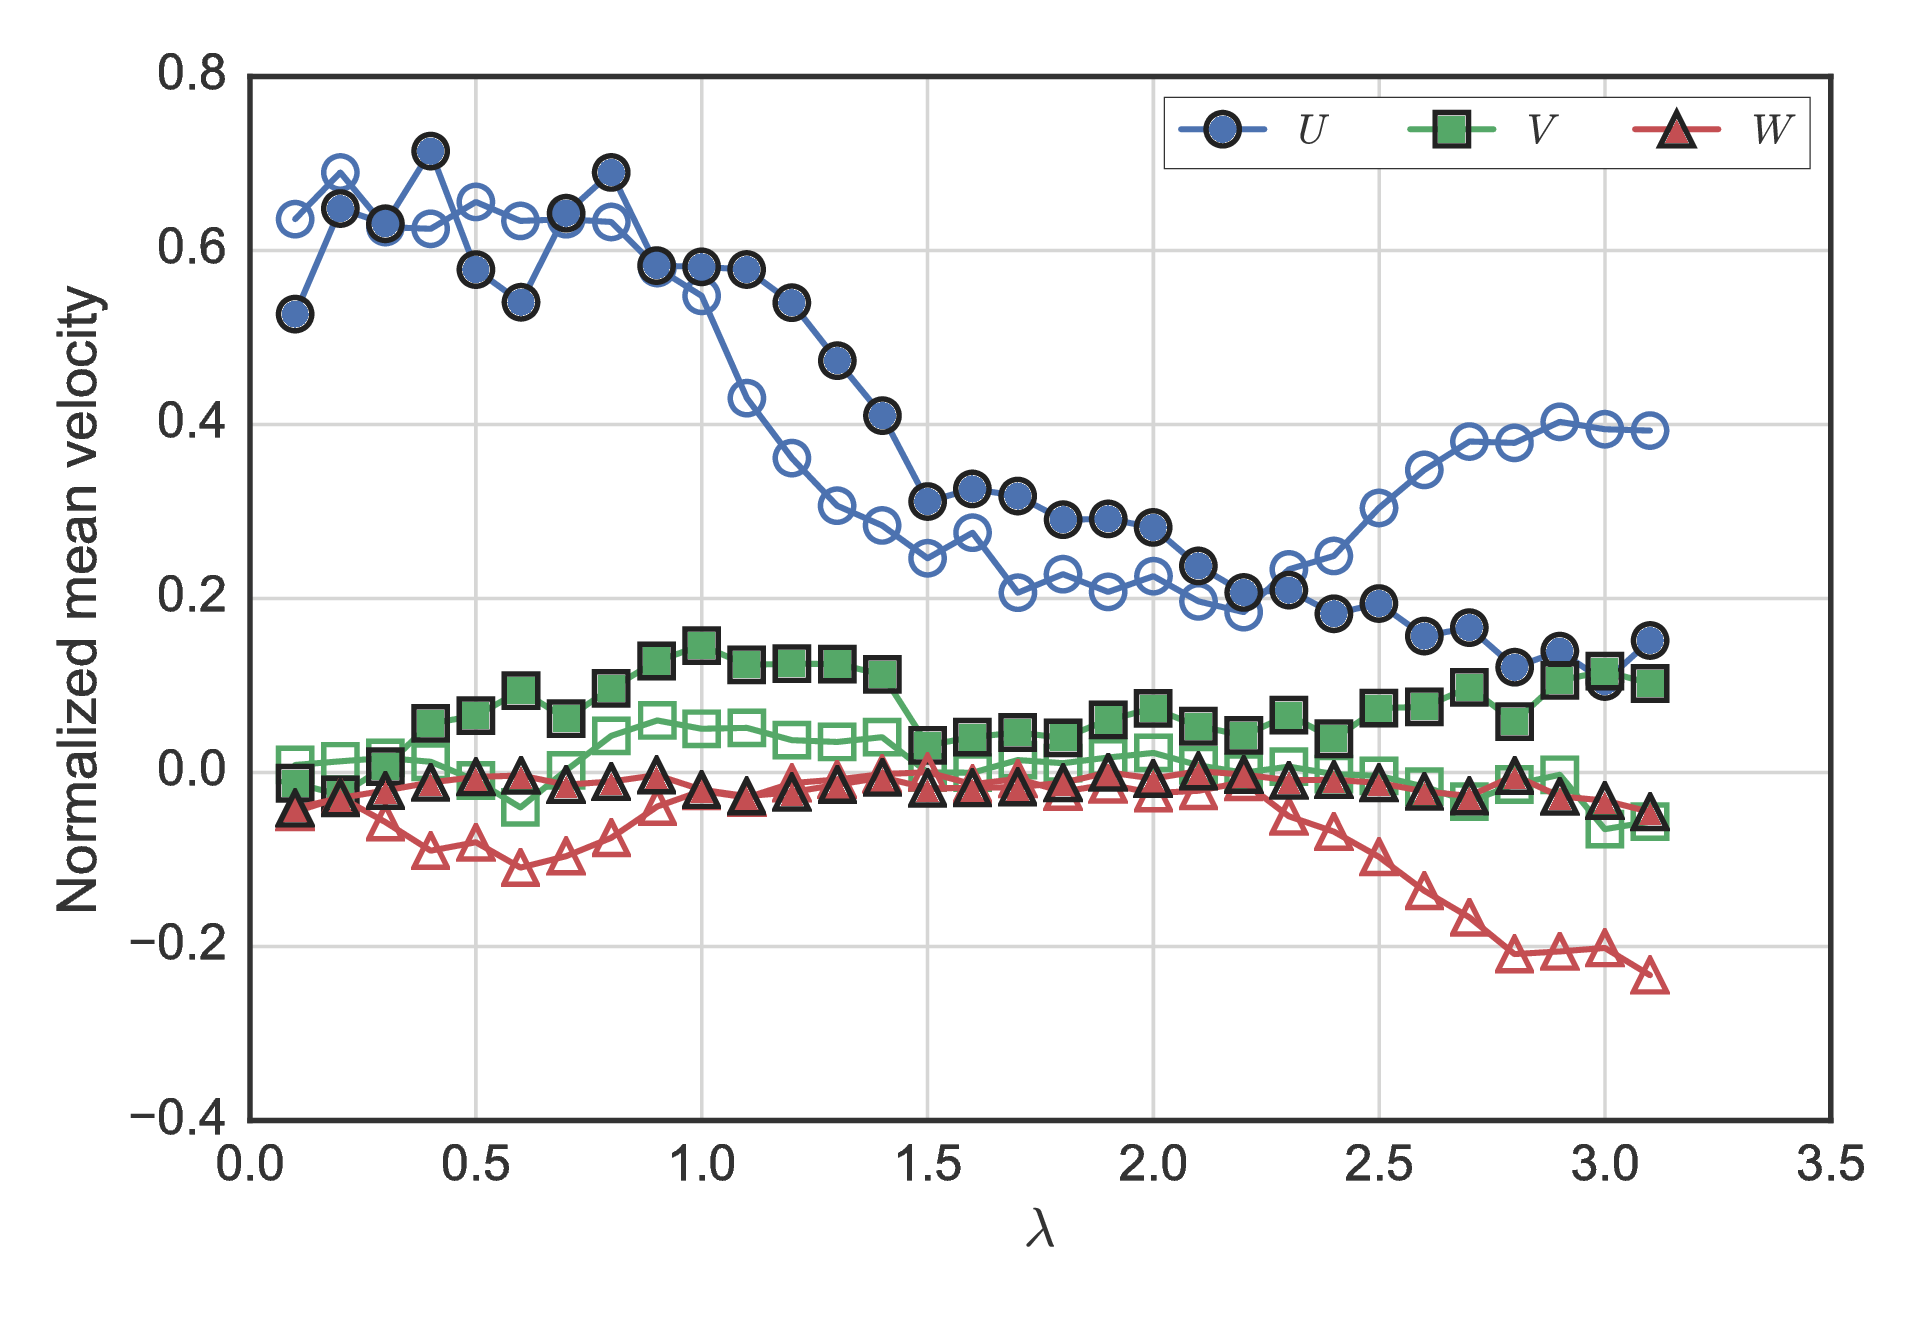
\includegraphics[width=0.75\textwidth]{RVAT-baseline_mean_vel_vs_tsr}

    \caption{Normalized centerline mean velocity components at $x/D=1$ versus
        tip speed ratio. Filled markers indicate measurements at $z/H=0$, while open
        markers indicate those at $z/H=0.25$.}

    \label{fig:RVAT-baseline-mean-vel-vs-tsr} 
\end{figure}

Next we want to look more closely at the effects of lowering $\lambda$, thereby
increasing maximum blade angle of attack and inducing increased stalling
behavior. Quarter height streamwise mean velocity profiles for the two tip speed
ratios of interest are shown in Figure~\ref{fig:RVAT-baseline-meanu-2tsrs}. Some
similarities can be identified with the study by Brochier \etal, namely the
assymetry of the mean velocity profile and how its shape changes on the side of
the turbine where the blade faces into the flow---positive $y$ for our
experiments and negative for theirs~\cite{Brochier1986}.

Figure~\ref{fig:RVAT-baseline-meanw-2tsrs} shows mean vertical velocity profiles
for the two tip speed ratios of interest. The large gradient appearing at
negative values of $y$, suspected to be the result of blade tip vortices,
remains a approximately the same location. However, the peak seen at $y/R = 1.2$
is decreased for the lower tip speed ratio case.

Figure~\ref{fig:RVAT-baseline-meanv-2tsrs} shows profiles of mean cross-stream
velocity for both $\lambda$ values. Unlike the streamwise and vertical profiles,
these show relatively large differences at our two tip speed ratios of interest,
indicating significant fluid motion---on the order of 10\% of the free stream
velocity---to the left on the left edge of the rotor at $\lambda=1.9$ and to the
right at the right edge of the rotor at $\lambda = 1.4$. This shows how by
changing tip speed ratio, and therefore the location of peak blade loading,
there may be potential for control over transverse diversion of the flow in the
near-wake.

Regarding turbulence kinetic energy in the wake, profiles of which for the two
tip speed ratios are shown in Figure~\ref{fig:RVAT-baseline-k-2tsrs}, we can
make similar comparisons with the very low $Re$ study of Brochier
\etal~\cite{Brochier1986}. Their results show two peaks on opposite sides of the
rotor axis, with the lower tip speed ratio case having a relatively higher peak
on one side, which should correspond to negative $y$ values in our case. This is
somewhat in agreement with our results, though the value at the origin for our
case is relatively higher, which may be due to the larger shaft wake. However,
when we compare our two profiles, we notice for the lower value of $\lambda$
there is higher average turbulence levels throughout the center region. This
appears to be caused by more intense blade stall, beginning earlier along the
upstream blade path, i.e., at higher positive values of $y$.

\begin{figure}
    \centering
    
    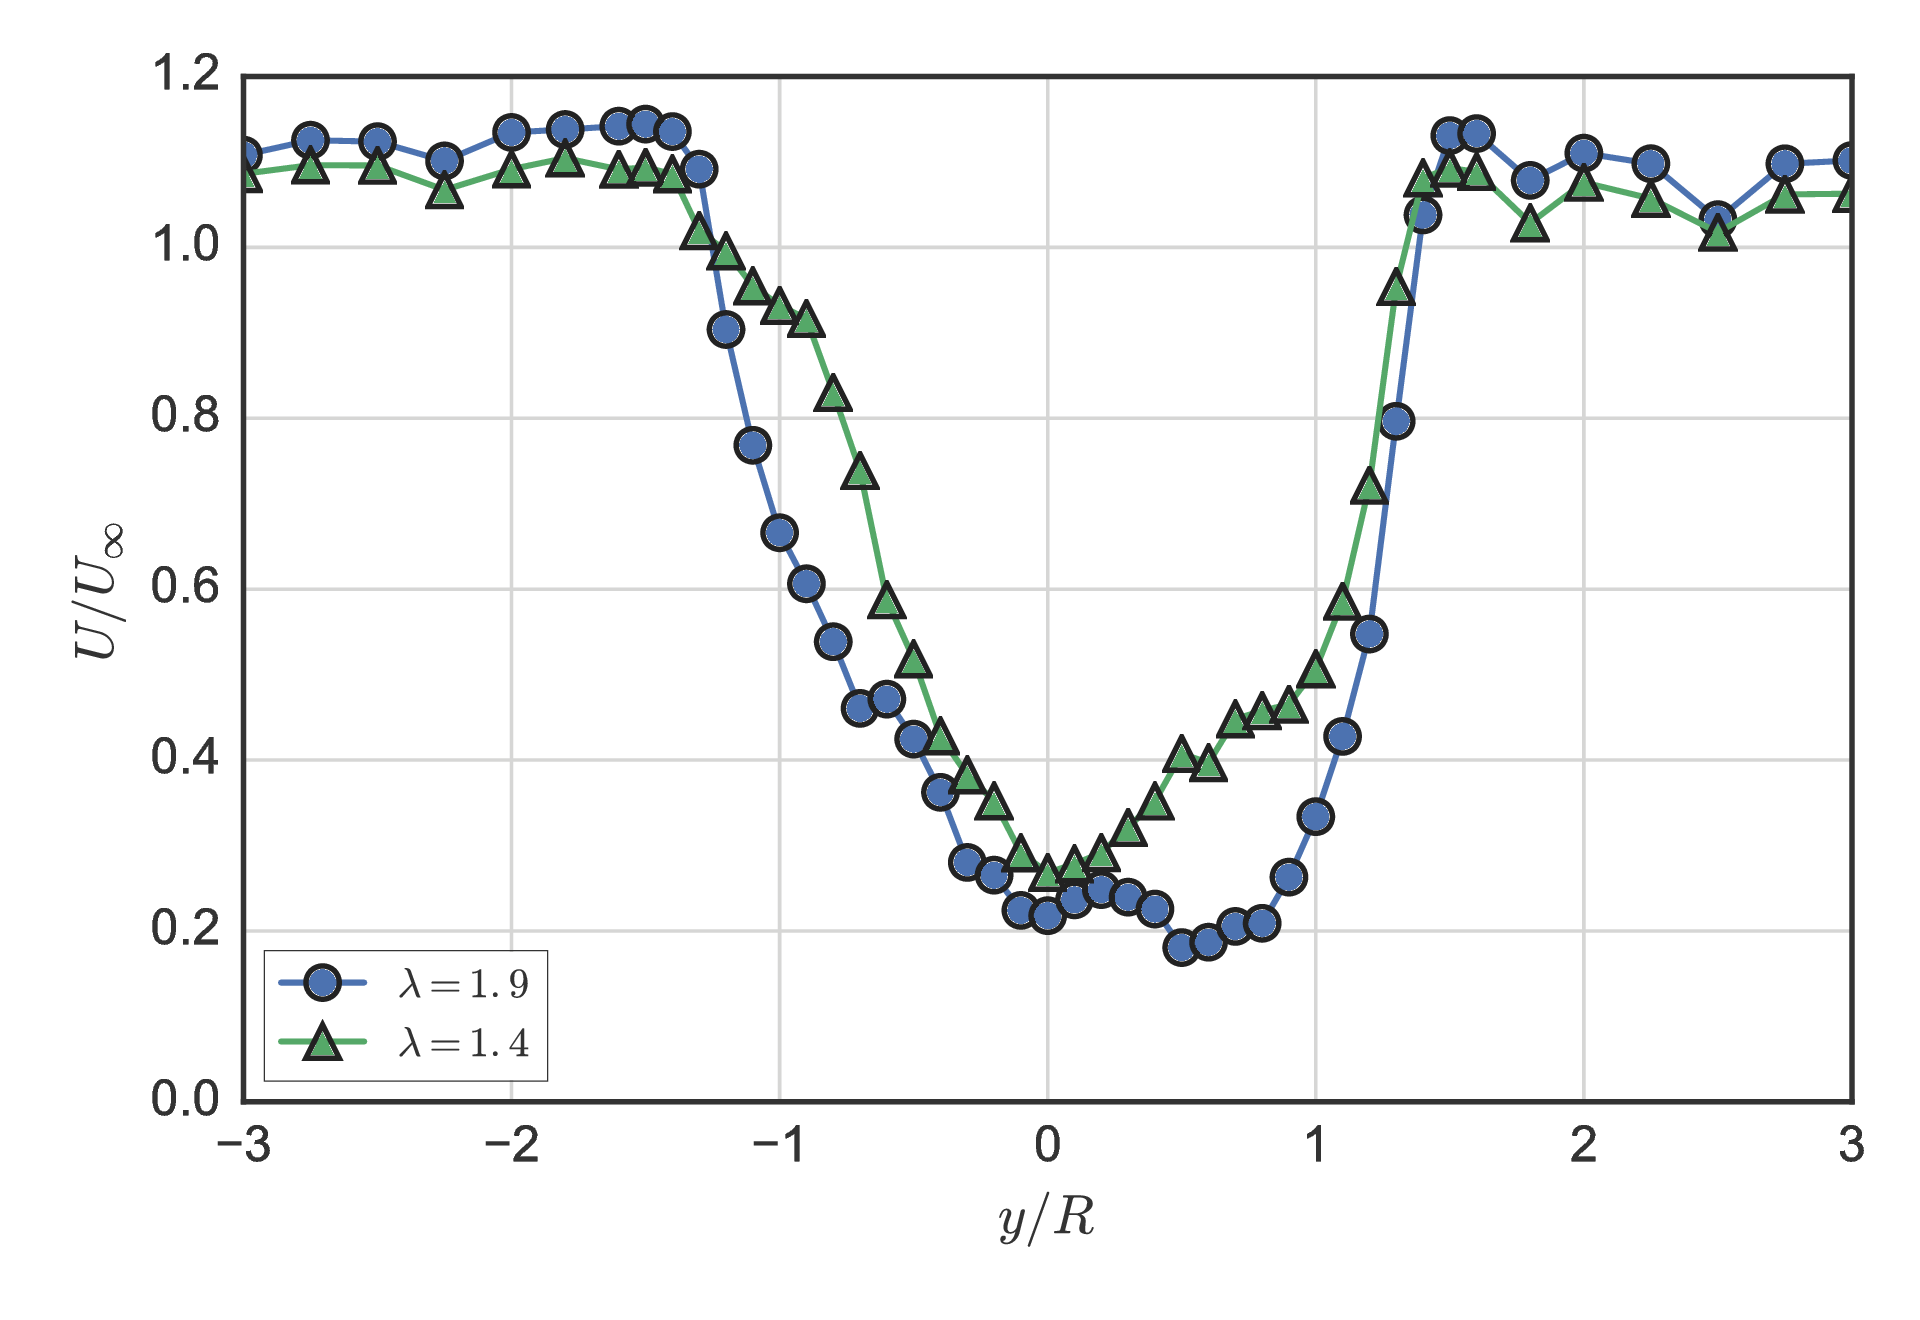
\includegraphics[width=0.75\textwidth]{RVAT-baseline_meanu_2tsrs}

    \caption{Streamwise mean velocity profiles for $\lambda = 1.9$ and
        $\lambda=1.4$ at $x/D=1$ and $z/H = 0.25$.}

    \label{fig:RVAT-baseline-meanu-2tsrs} 
\end{figure}

\begin{figure}
    \centering
    
    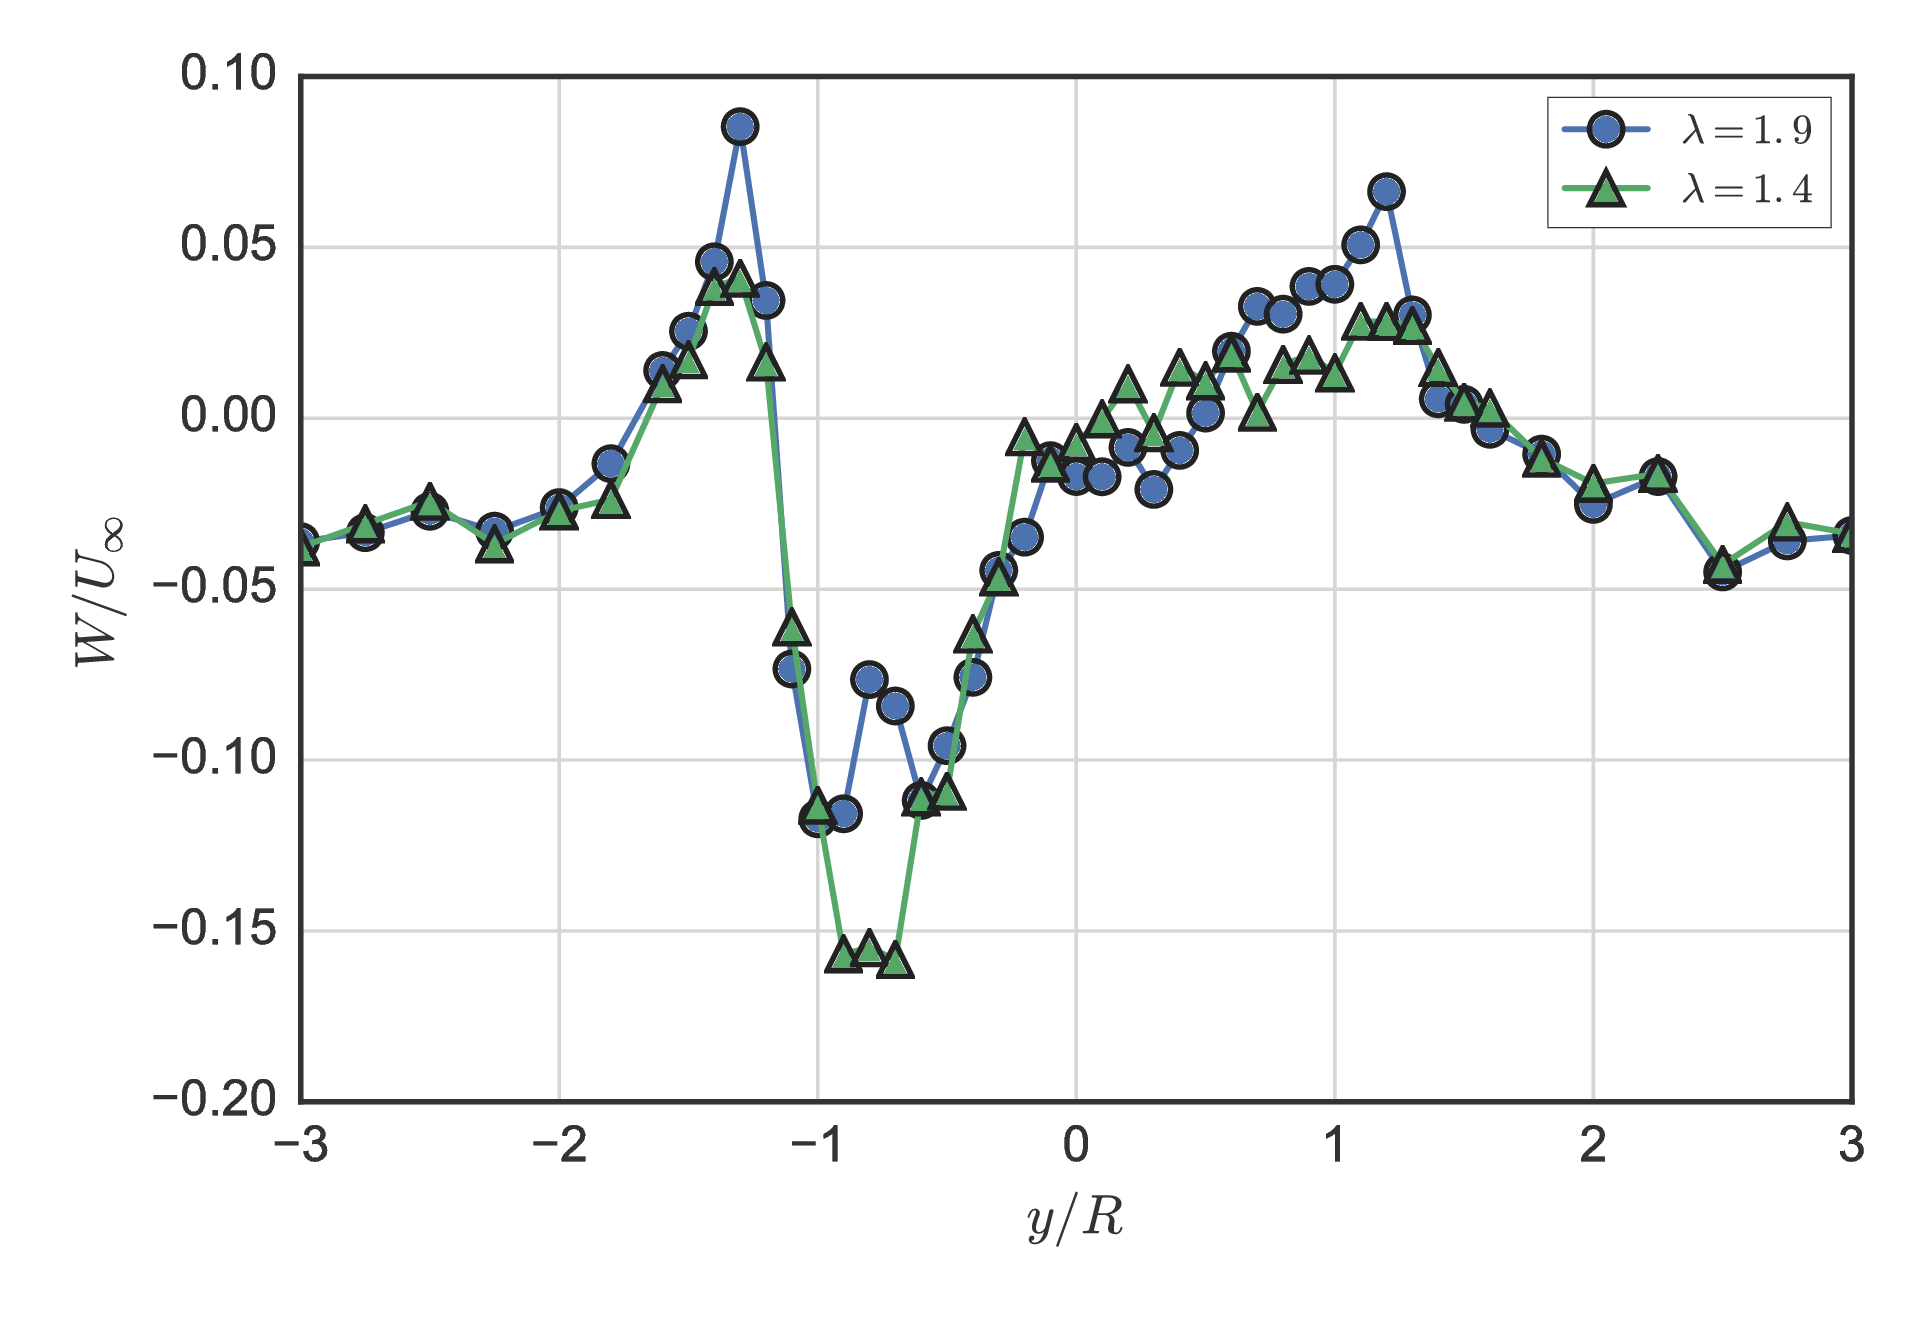
\includegraphics[width=0.75\textwidth]{RVAT-baseline_meanw_2tsrs}

    \caption{Mean vertical velocity profiles for $\lambda = 1.9$ and
        $\lambda=1.4$ at $x/D=1$ and $z/H = 0.25$.}

    \label{fig:RVAT-baseline-meanw-2tsrs} 
\end{figure}

\begin{figure}
    \centering
    
    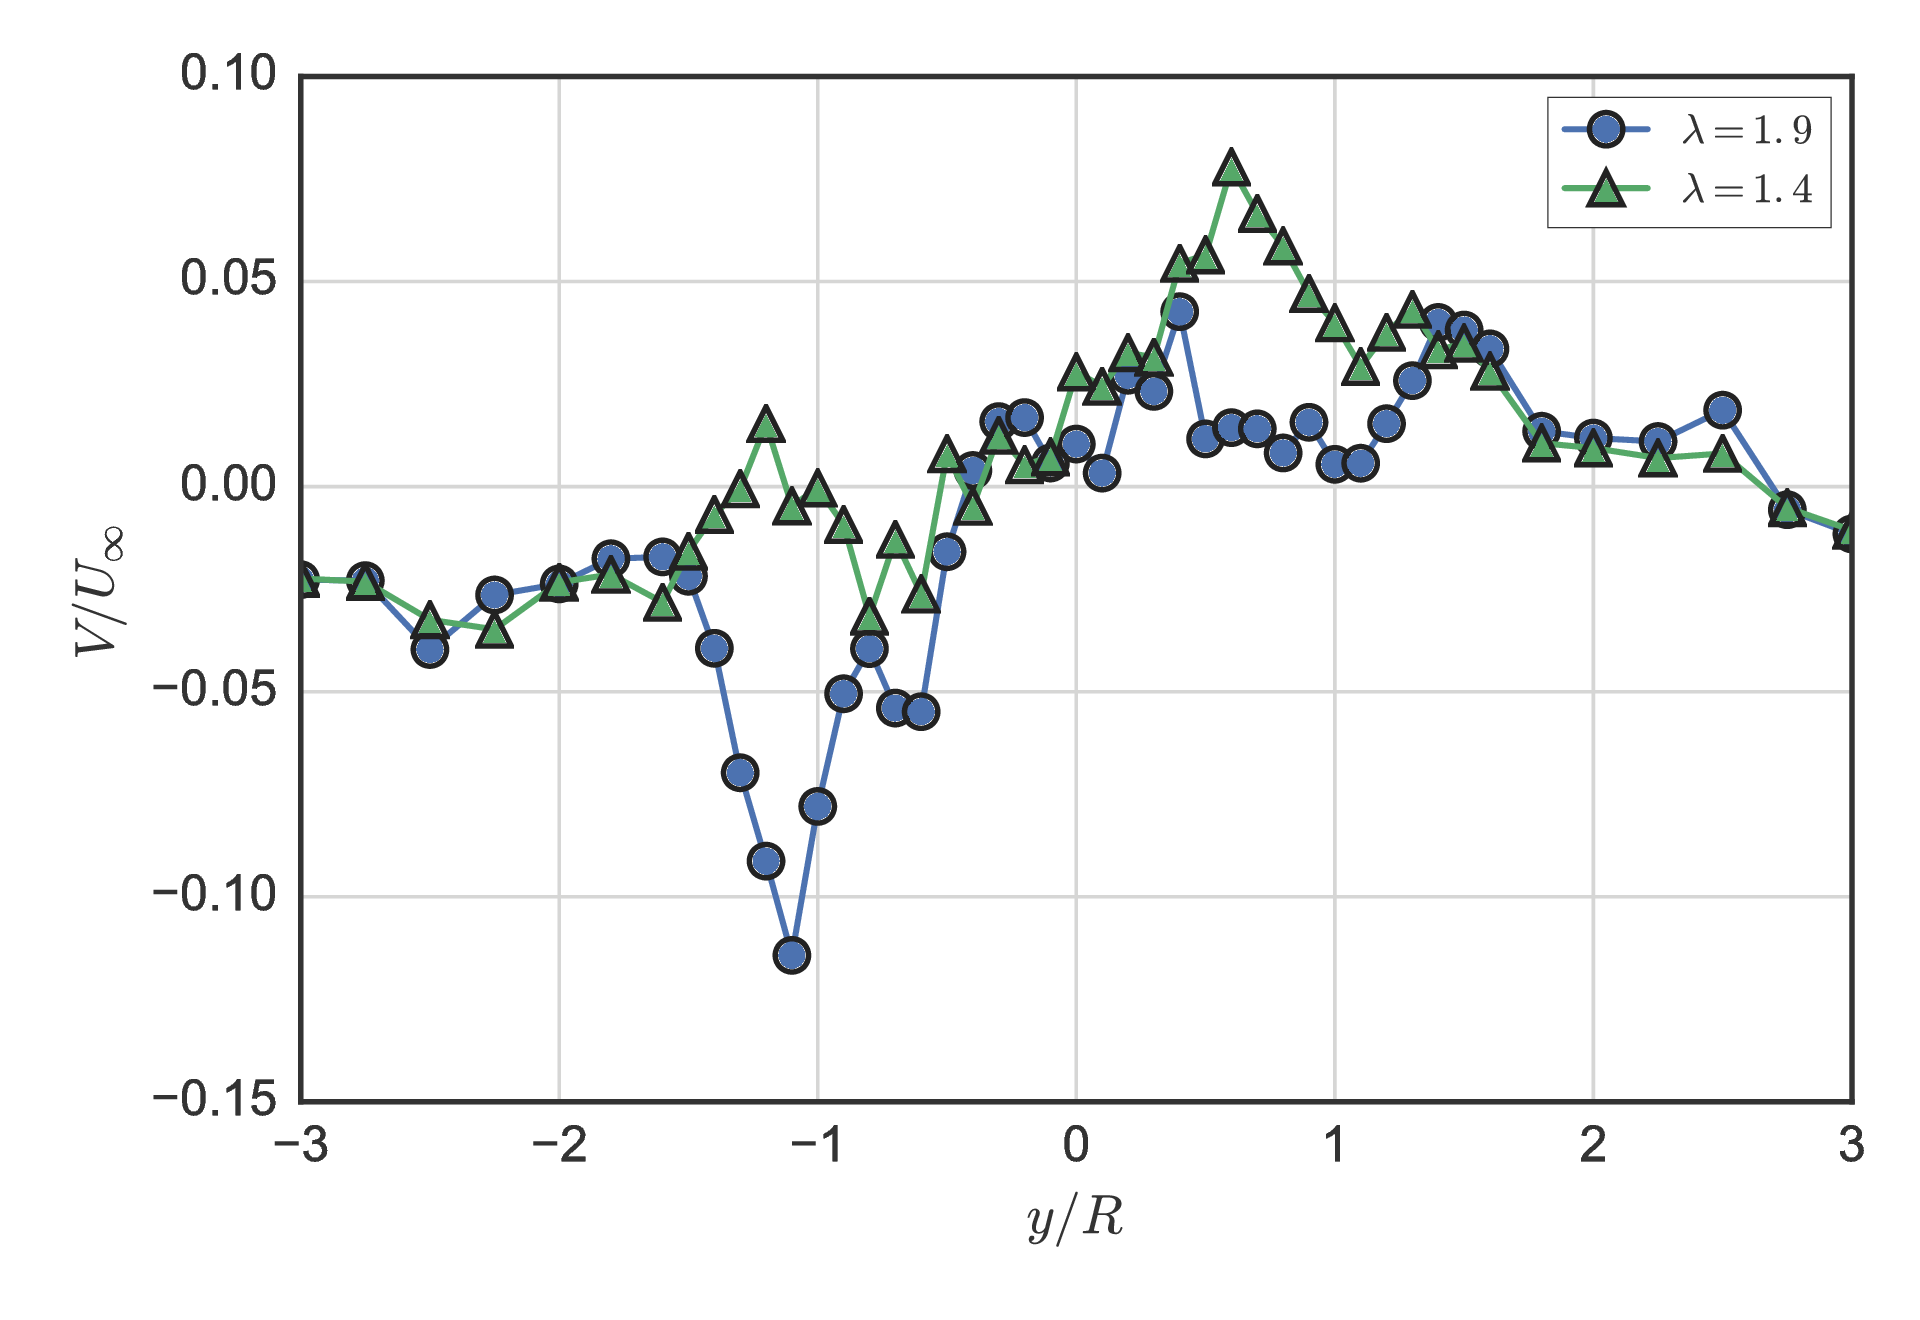
\includegraphics[width=0.75\textwidth]{RVAT-baseline_meanv_2tsrs}

    \caption{Mean cross-stream velocity profiles for $\lambda = 1.9$ and
        $\lambda=1.4$ at $x/D=1$ and $z/H = 0.25$.}

    \label{fig:RVAT-baseline-meanv-2tsrs} 
\end{figure}

\begin{figure}
    \centering
    
    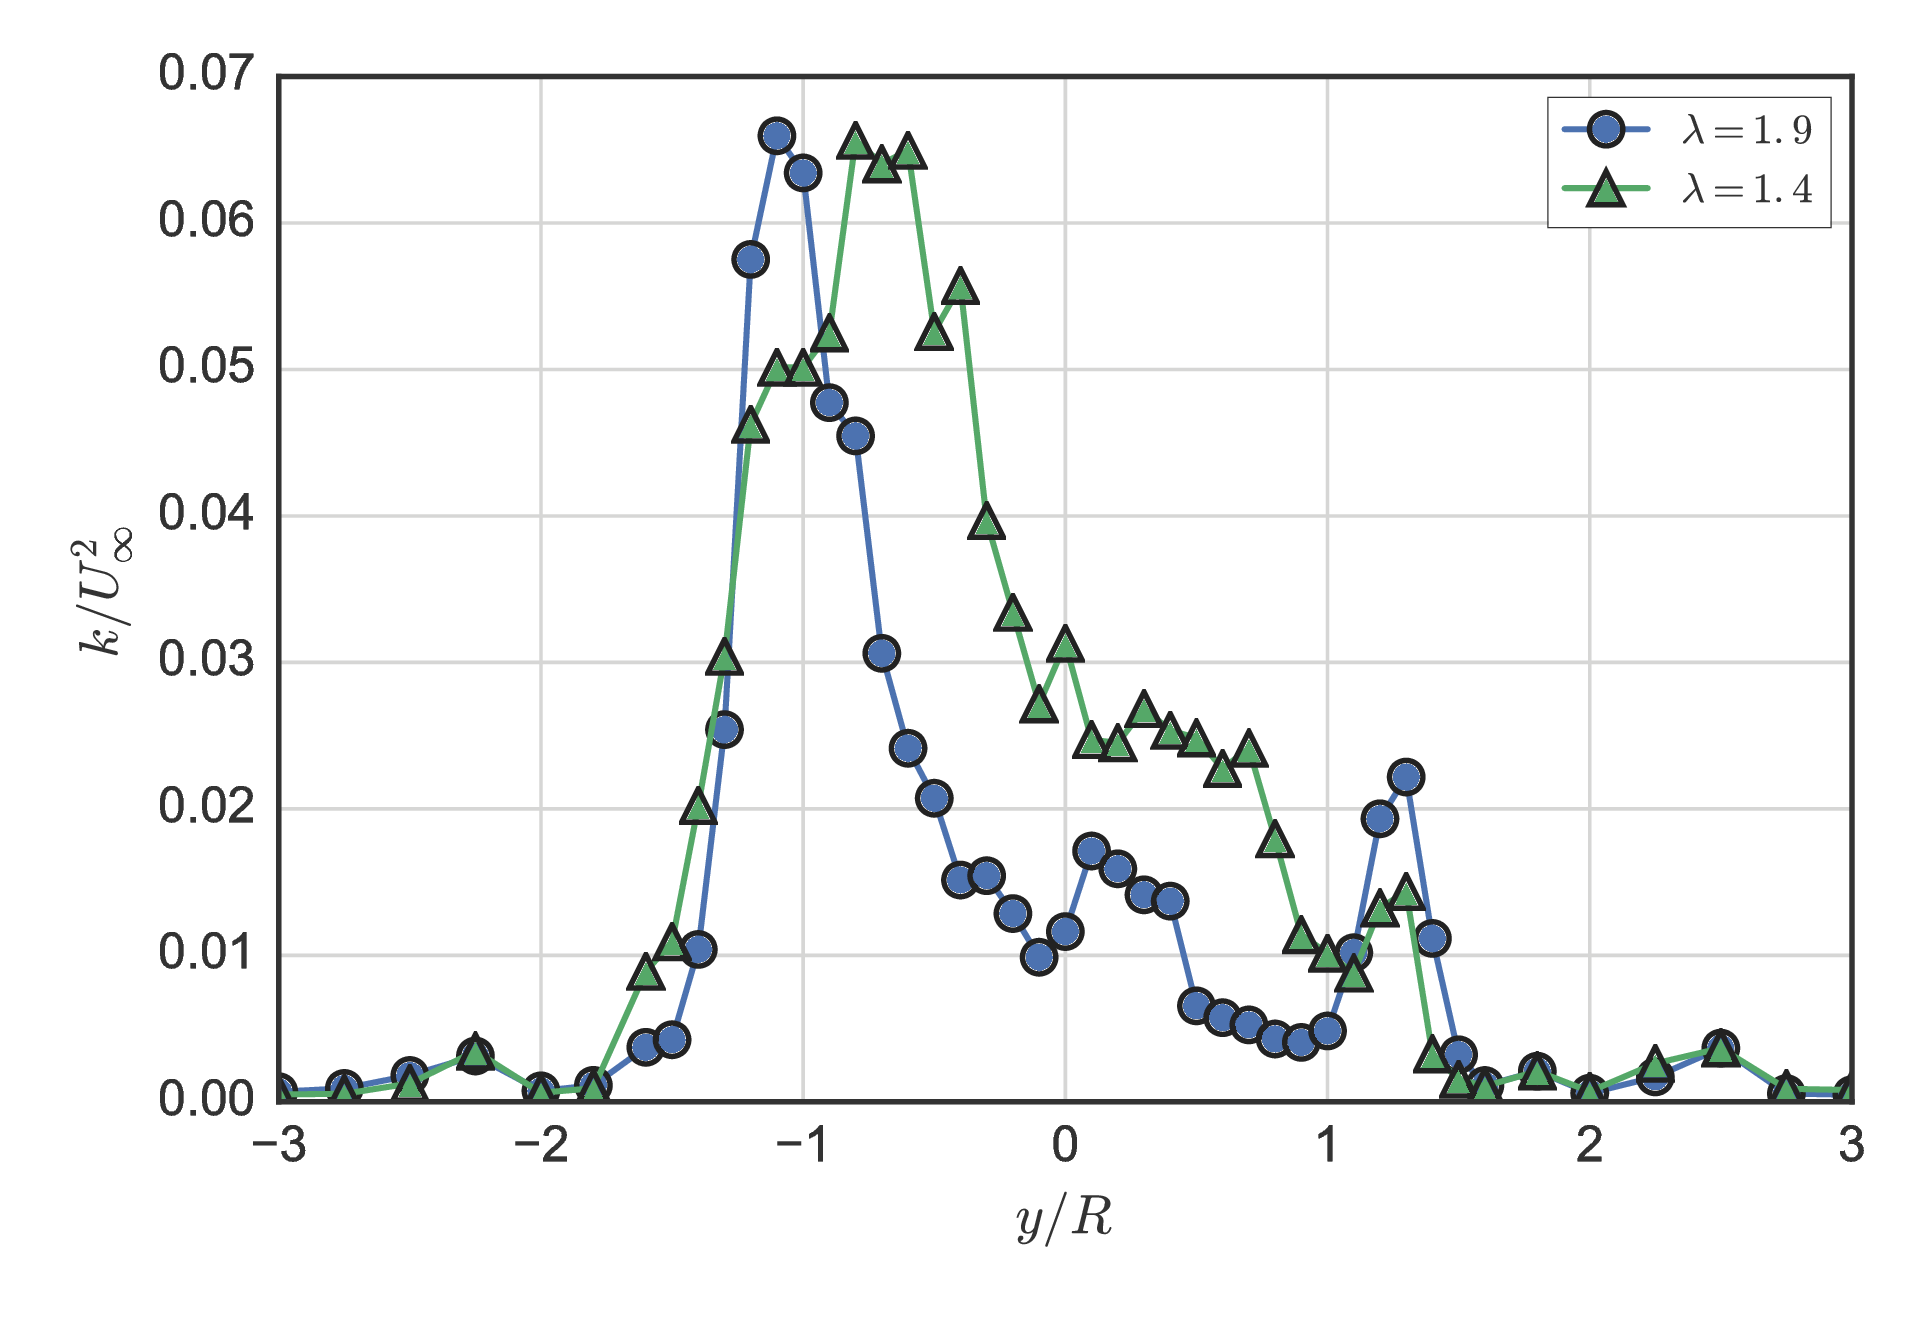
\includegraphics[width=0.75\textwidth]{RVAT-baseline_k_2tsrs}

    \caption{Turbulence kinetic energy for $\lambda = 1.9$ and
        $\lambda=1.4$ at $x/D=1$ and $z/H = 0.25$.}

    \label{fig:RVAT-baseline-k-2tsrs} 
\end{figure}


\subsection{Comparison with an actuator disk}

The actuator disk model, commonly used in modern large-eddy simulations of wind
farms \cite{Stevens2014}, parameterizes turbine forcing on the flow field as a
steady streamwise force applied over the frontal area of the turbine. The model
is attractive due to its relatively simple implementation; it does not require
the meshing of actual turbine geometry, making it computationally feasible to
simulate large turbine arrays. For example, the turbine array being installed by
ORPC in Cobscook Bay, Maine was laid out with a RANS actuator disk model, where
cross-flow turbines were represented inside the mesh over three cells
\cite{Nelson2013}. Furthermore, the actuator disk force coefficients are not
time dependent, allowing for simulation of, e.g., tidal cycles without the need
for small time steps to resolve unsteady turbine forcing.

Here the experimental measurements are compared and contrasted with the
near-wake of an actuator disk model, to illustrate how this model would
represent a cross-flow turbine in an array simulation. Since one of the
potential benefits of cross-flow turbines is to be able to be spaced more
closely in an array installation, the near-wake dynamics will be more important
than those of an axial-flow turbine.

For axial-flow turbines, the actuator disk model can be enhanced with a rotating
axial velocity component, which gives better results than a simple volume force
\cite{Wu2011}, but to our knowledge this technique has not been applied
(adapted) to cross-flow turbines. Nevertheless, in the present study the
ability of a simple streamwise force distributed over a cylindrical volume to
mimic the near-wake of a cross-flow turbine was evaluated. As described in
previous sections, the asymmetry of the turbine's wake indicates that a uniform
streamwise force from the actuator disk will likely not capture the wake
accurately.

\todo[inline]{Check OpenFOAM version used for AD simulation.}

The open source CFD package \textit{OpenFOAM} was used to solve the RANS
equations with the turbine represented by an actuator disk, which is
implemented as a force or sink in the momentum equation, applied over a selected
volume of cells in the mesh.

The cross-section of the domain is the same as that of the tow tank used for the
experimental measurements. The actuator disk is technically not a disk, but a 1
m diameter by 1 m tall cylinder, mimicking the turbine swept area. The domain
extends 2 m upstream and 8 m downstream.  The background mesh consists of 96,
64, and 48 points in the $x$, $y$, and $z$ directions, respectively. The cells
in the volume enclosed by the actuator disk region are refined by a factor of
two, giving a total of  approximately $3 \times 10^5$ hexahedral cells. A
snapshot of the mesh is shown in Figure~\ref{fig:AD-mesh}. Boundary conditions
are set to approximate the tow tank environment, i.e., the velocity at the
bottom and walls is set to the free stream value. The free surface was not
modeled---the domain had a rigid lid with a slip velocity boundary condition---a
reasonable approximation for low Froude numbers. Inputs to \textit{OpenFOAM}'s
\texttt{actuationDiskSource} are given in Table~\ref{tab:AS}, and the case files
for this simulation are available from \cite{Bachant2014-OF-AS-case-files}.

\begin{figure}
    \centering

    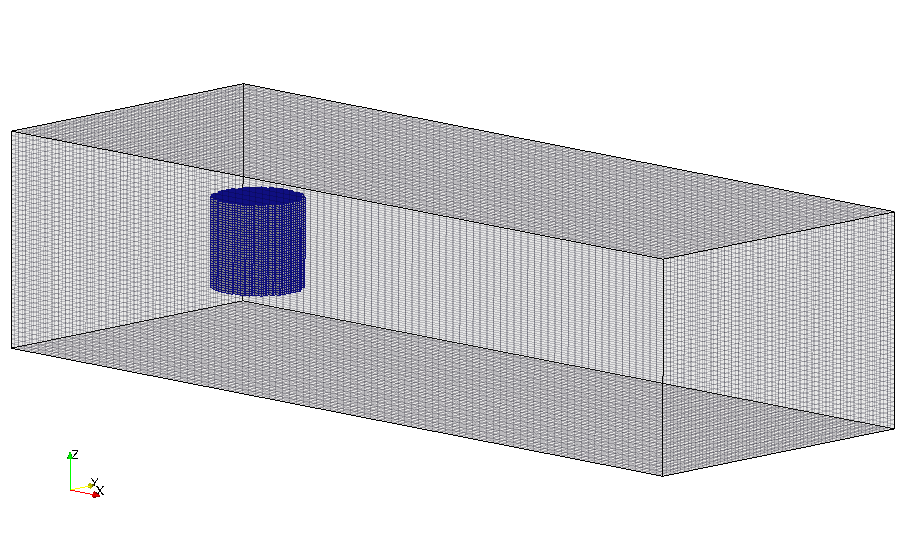
\includegraphics[width=0.9\textwidth]{AD_mesh}

    \caption{Snapshot of the computational mesh for the actuator disk RANS
        simulation.}
    
    \label{fig:AD-mesh}
\end{figure}

\begin{table}
    \begin{center}
        \begin{tabular}{r|l}
            \texttt{Cp} & \texttt{0.26} \\ 
            \texttt{Ct} & \texttt{0.96} \\ 
            \texttt{diskArea} & \texttt{1.0} \\ 
            \texttt{upstreamPoint} & \texttt{(-1.0 0 0)} \\ 
        \end{tabular} 
        \caption{Input parameters for the actuator surface using \textit{OpenFOAM}'s
            \texttt{actuationDiskSource}.}
    \label{tab:AS}
    \end{center}
\end{table}

The turbulence is modeled with a standard $k$-$\epsilon$ closure, with
relatively low levels of inlet turbulence kinetic energy and dissipation, $2
\times 10^{-4}$ and $3 \times 10^{-5}$, respectively. These low free stream
values were chosen to approximate the tow tank ambient conditions.

Results for the mean velocity field are presented in
Figure~\ref{fig:AD-contours}, in a manner similar to that of
Figure~\ref{fig:RVAT-baseline-meancontquiv}, for comparison. The vertical mean
flow, which was determined to be an important driver of near-wake dynamics in
the experiments, is absent. In fact, it contributes negatively to streamwise
wake recovery. This means that all momentum and energy transport back into the
deficit in the wake created by the turbine will need to be facilitated by
turbulent transport (and viscous diffusion, to a much lesser degree). Note also
how acceleration due to blockage is much lower compared to the experiments
despite matching the overall drag coefficient.

Figure~\ref{fig:AD-streamwise} shows the downstream evolution of the centerline
streamwise velocity, and the terms that contribute to its streamwise derivative
averaged over various constant-$x$ planes. Note how very close to the turbine,
the streamwise pressure gradient is contributing significantly to the increase
in $U$, despite the fact that the turbine creates a positive pressure gradient
along the centerline. The large pressure-driven increase in streamwise velocity
makes sense considering the fact that the values are averaged over the entire
cross-section of the domain, which includes a large area of flow acceleration
around the turbine, where the streamwise pressure gradient is negative. Just
after the turbine, $-\p P / \p x$ drops off very quickly and then acts to
decrease streamwise momentum slightly as the static pressure recovers moving
downstream.

We can see that the streamwise momentum recovers very slowly, only starting to
recover around $x=7D$, which can be mostly attributed to the low inflow
turbulence levels, chosen to mimic the tow tank environment. This can be further
understood by looking at the transport terms plotted on the right in
Figure~\ref{fig:AD-streamwise}, where we see all terms are quite small when
compared with the experimental results from the turbine. Rather than the
advection terms, which contribute negatively, the turbulent transport---here
modeled using the $k$--$\epsilon$ eddy viscosity $\nu_t$---is driving the
streamwise evolution, despite being very small. One way to increase the wake
recovery in such a model is to have the actuator disk ``inject'' turbulence
quantities to increase the eddy viscosity \cite{James2011, Nelson2013}. However,
this will likely still not be sufficient to predict evolution and interaction in
closely-spaced arrays of CFTs, since neither the significant vertical mean 
velocities in the CFT wake, nor any coherent vortical structures 
due to blade, shaft, or strut forces are captured by the actuator disk model.

It could be argued that the actuator disk model should not be judged this way as
it is well known that it is a poor predictor of near-wake characteristics,
however, these models are common in engineering practice when calculating
performance of turbine arrays, as previously mentioned. The experiments reported
here have shown that the use of these models would likely be a source of large
uncertainty if applied to cross-flow turbine installations.

\begin{figure}
    \centering
    
    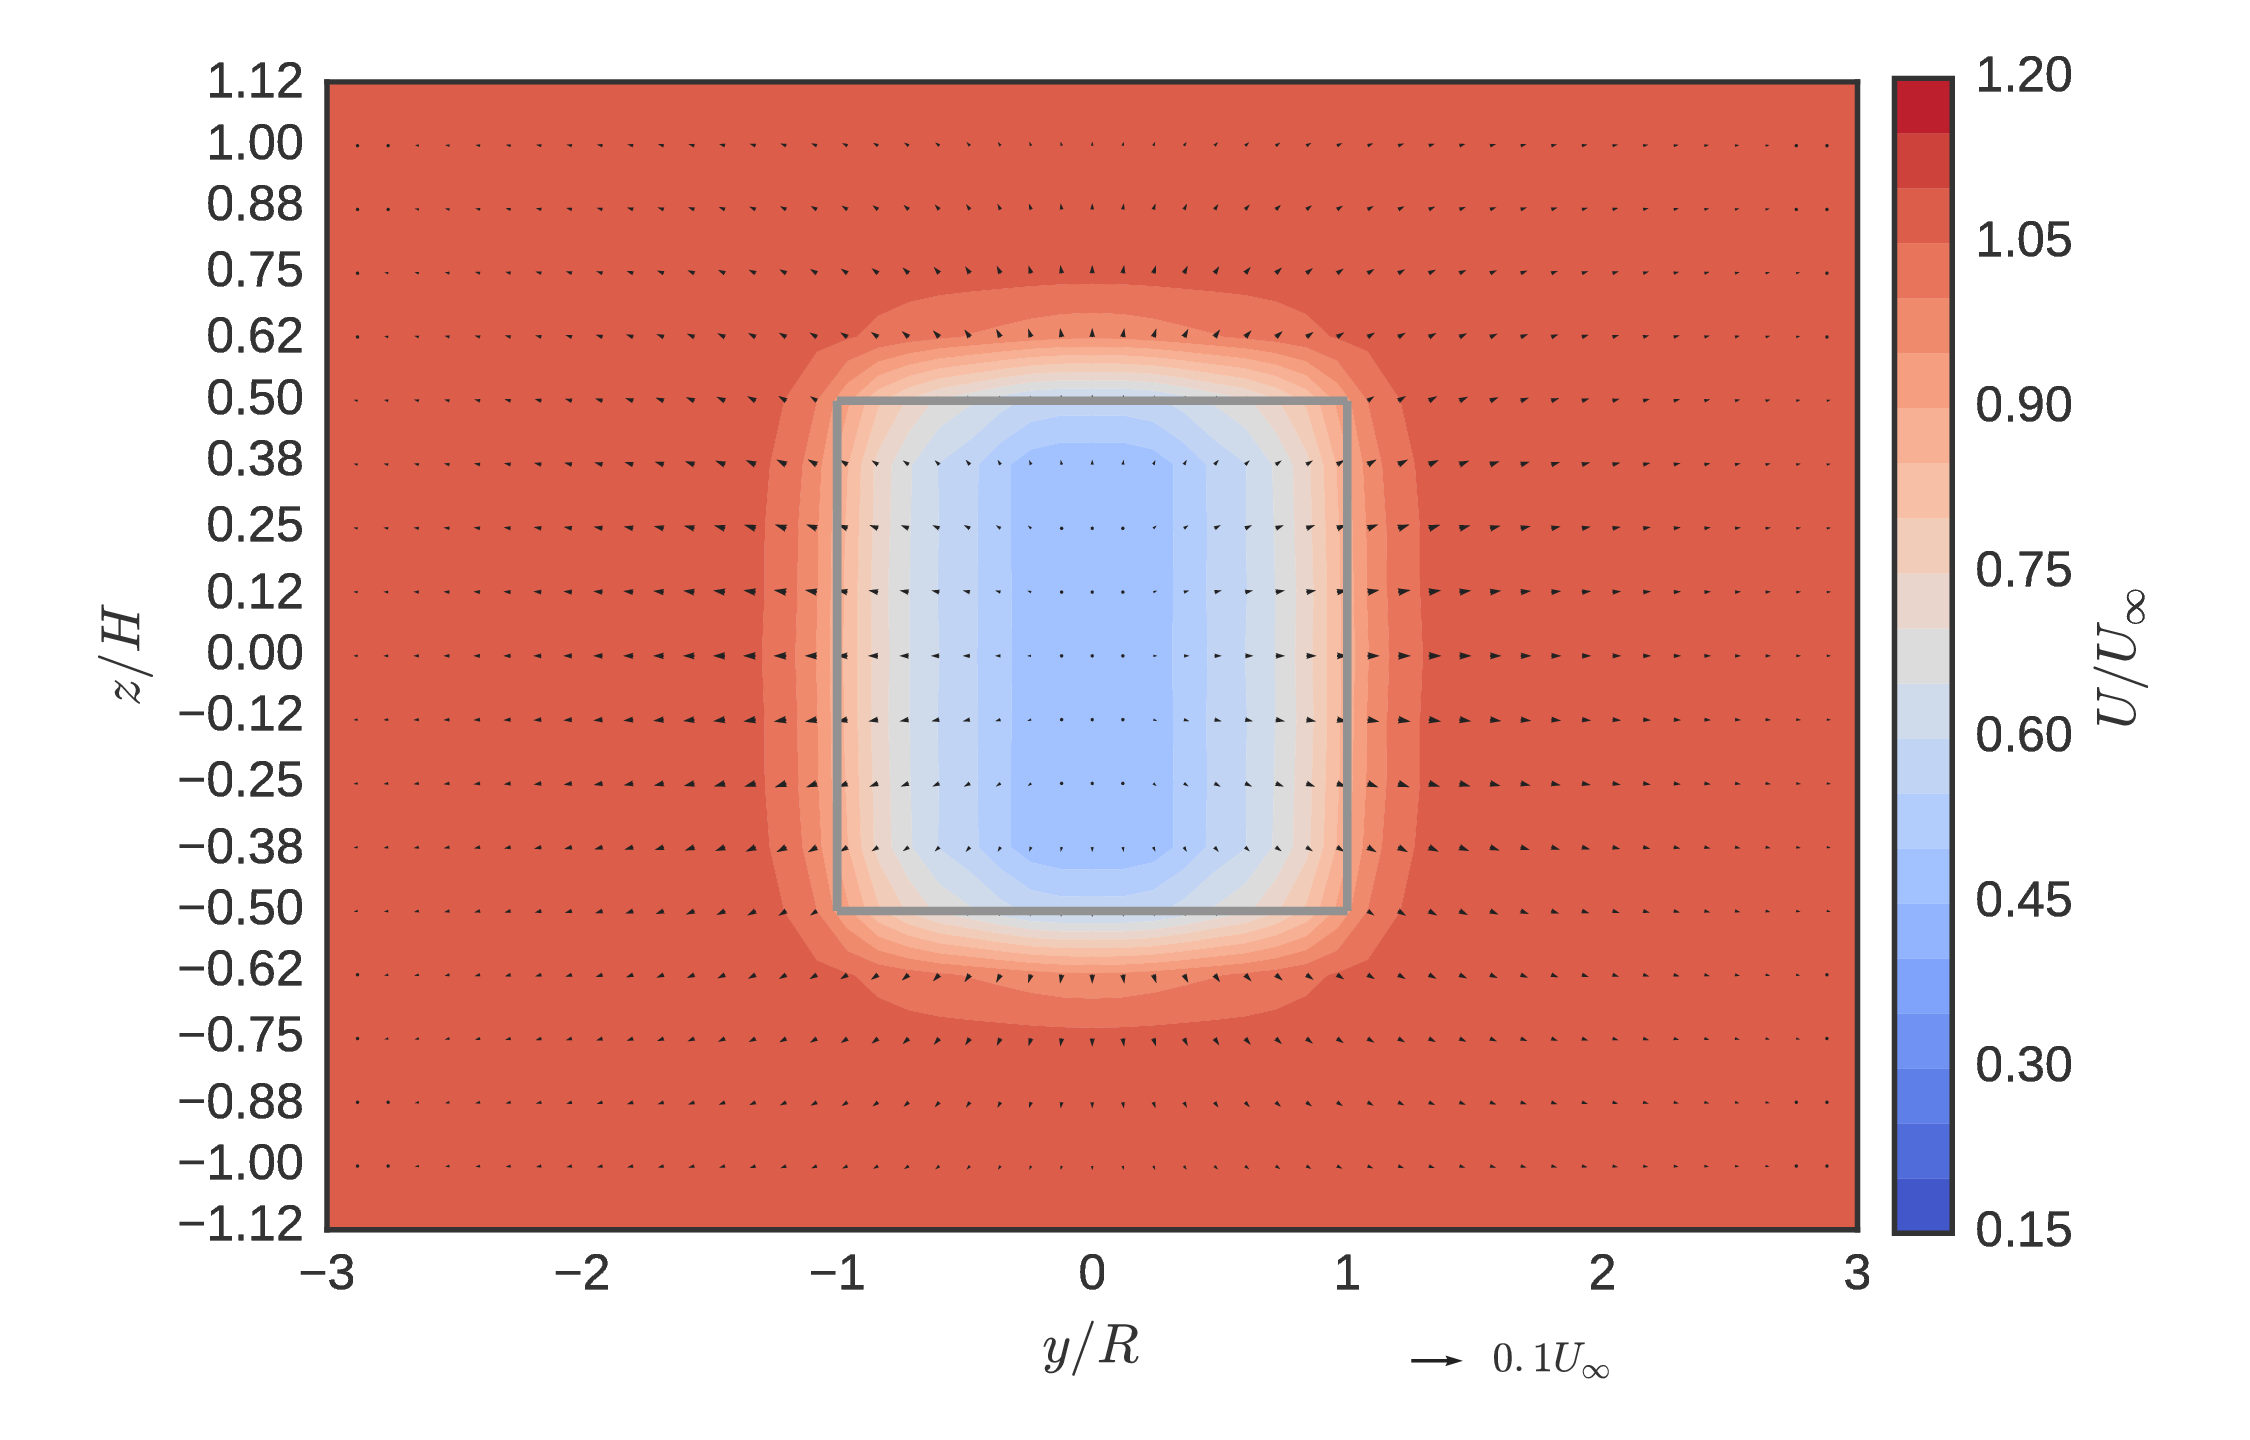
\includegraphics[clip, trim=0 0.25in 0 0.5in,
    width=0.75\textwidth]{AD_meancontquiv}

    \caption{Mean velocity predictions at $x/D=1$ from the RANS actuator disk
        numerical model. Vectors are cross-stream and vertical velocities; contours
        are streamwise velocity.}
    
    \label{fig:AD-contours}
\end{figure}

\begin{figure}
    \centering 
    
    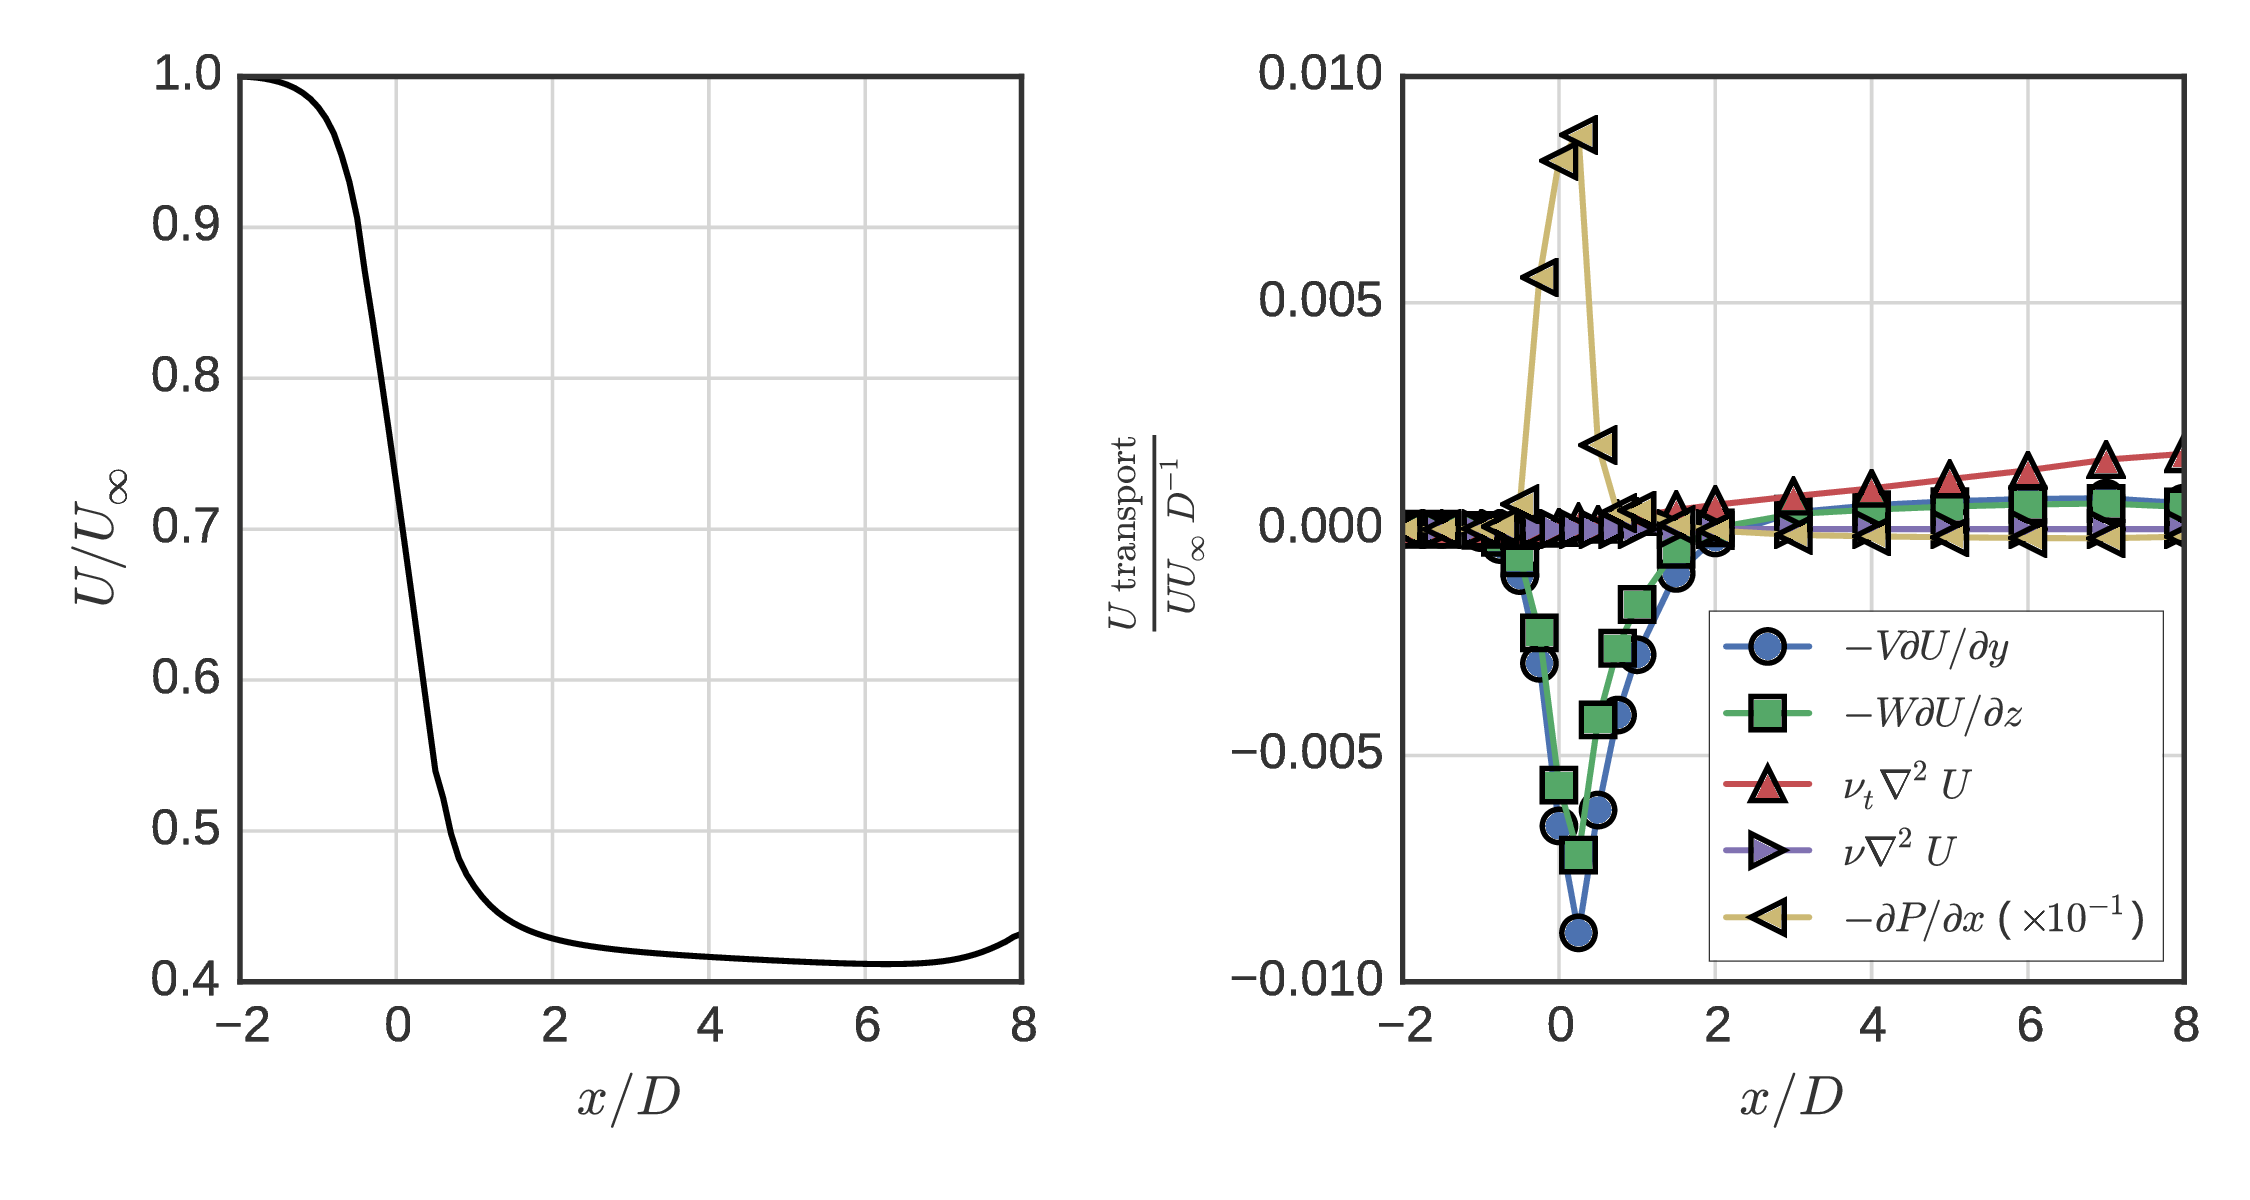
\includegraphics[width=0.9\textwidth]{AD_streamwise}
    
    \caption{Downstream evolution of the centerline streamwise velocity (left)
        and normalized momentum transport terms (right) averaged over $y$--$z$
        slices from the actuator disk RANS simulation.} 
    
    \label{fig:AD-streamwise}
\end{figure}

\section{Conclusions}

Detailed measurements were performed in the near-wake of a vertical axis
cross-flow turbine operating at peak power coefficient. The following essential
features were identified:

\begin{enumerate}
    \item Asymmetry and three-dimensionality in the mean velocity field. 
    
    \item Mean streamwise swirling flow, or vorticity produced by blade tip and
    dynamic stall vortex shedding, which propels fluid towards the wake's center
    and makes mean vertical advection the largest contributor to streamwise
    momentum and mean kinetic energy recovery.
    
    \item Asymmetric turbulence generation due to the effects of dynamic stall
    being more pronounced on one side of the turbine.
\end{enumerate}

The most dominant timescale induced into the wake is the blade passage period. 
The $+y$ side of the turbine contains more coherent motion at this
frequency, as stalling is less prevalent there. The reduced separation due to 
stall also leads to lower magnitudes of turbulence kinetic energy on the $+y$ 
side. 

Regarding recovery of the mean streamwise momentum and kinetic energy, it was
calculated from the wake velocity measurements that vertical advection is more
than twice as large as transport by turbulent fluctuations, which may explain
why CFT wakes entrain free stream kinetic energy more effectively than their AFT
counterparts. The importance of the vertical flow created by the turbine showed
that array flow simulations will need to be carried out in three dimensions to
produce accurate results. Considering how high power coefficient estimates are
in 2-D simulations \cite{Li2013}, it logically follows that 3-D effects
significantly decrease the power output of a single turbine, but this uncaptured
power helps pull more power from outside the array. This also raises interesting
questions with respect to how cross-flow turbine blades should be
``terminated'', i.e., reducing blade tip vortices by winglets or inhibiting them
with end struts or end disks, as commonly done, may increase the performance of
individual CFTs, however, free ends that produce tip vortices may be
advantageous in an array setting to increase the wake recovery rate.
Furthermore, it hints at the possibility of using vortex generators might be
added to horizontal-axis or axial-flow turbines to help entrain more mean
kinetic energy from above.

A commonly used, simple turbine forcing parameterization---an actuator
disk---was assessed for predicting the near-wake characteristics of this turbine
with a RANS simulation. The actuator disk model was found to be a poor
representation of a CFT, despite its computational efficiency and use in
research and industry. It is suggested that an actuator disk with a non-uniform
force distribution or a collection of actuator lines~\cite{Sorensen2002,
    Shamsoddin2014} may produce the asymmetry and unsteadiness that is
characteristic of the CFT near-wake and will be necessary to predict performance
of closely-spaced arrays that cross-flow turbines are thought to enable. The
actuator line method is investigated later in Chapter~\ref{chap:ALM}.

% Chapter on Re dep experiments
\chapter{Reynolds number effects on the performance and near-wake of a high
solidity cross-flow turbine} \label{chap:Re-dep}

In this chapter, we will take a step back and investigate whether the results
from Chapter~\ref{chap:RVAT-baseline} were obtained at a large enough scale to
be considered relevant to full scale applications. Note that most of the content
here has been reproduced or adapted from~\cite{Bachant2016-Energies}.

Scaled physical models are often used in science and engineering to approximate
real-world systems. The principle of dynamic similarity allows for
geometrically-scaled systems to be dynamically identical if certain
nondimensional physical parameters are matched. In the case of fluid systems,
the most important nondimensional parameter is often the Reynolds number, $Re$,
which quantifies the importance of inertial forces over viscous forces on the
flow physics \cite{Acheson1990}: $Re = Ul/\nu$, where $U$ and $l$ are
characteristic velocity and length scales, respectively, and $\nu$ is the fluid
kinematic viscosity. The~other common dynamical scale, for systems with a free
surface, is the Froude number $Fr = U/\sqrt{gl}$, where $g$ is the gravitational
acceleration. Matching both the Froude and Reynolds number is not possible for a
scaled model in a given fluid, which is illustrated by the relation $Re =
l^{3/2} g^{1/2} Fr / \nu$, since $Re$ scales linearly with $l$, or the geometric
scale. In general, the geometric scale of a physical model is not necessarily
the same as its dynamical scale. As such, hereafter, we will use the word
``scale'' to refer to this dynamical scale or the Reynolds number and assume the
Froude number is small enough to be negligible.

With regards to wind and marine hydrokinetic (MHK) turbines, scaled physical
models are used to validate predictive numerical models, predict full-scale
performance of individual turbines and design or investigate arrays of devices.
Scaled models have the benefit of being significantly less expensive; however, a
key question is whether or not an acceptable scale mismatch exists.
Similarly,~it is questionable whether numerical models validated with physical
model data obtained orders of magnitude away from prototype scale should be
considered validated at all. An example of the errors that can result from the
extrapolation of small-scale experiments can be found in \cite{Baker1991}.

The performance and wake characteristics of cross-flow (often vertical-axis)
turbines (CFTs) depend on turbine solidity, blade profile (lift/drag, dynamic
stall at reduced frequency of turbine rotation, symmetry, thickness, camber),
blade pitch, number of blades, strut drag, operational parameters, such as tip
speed ratio, and on the Reynolds number \cite{Para2002}. Note that an average
blade chord Reynolds number, $Re_{c,\mathrm{avg}} \approx \lambda U_\infty c/
\nu$, can be expressed in terms of tip speed ratio $\lambda = \omega R/
U_\infty$, where $U_\infty$ is the free stream velocity, $c$ is the blade chord
length, $\nu$ is the fluid kinematic viscosity, $\omega$ is the rotor's angular
velocity, and $R$ is the rotor radius. The value of $\lambda$ at which a turbine
reaches peak performance in general decreases with turbine solidity $Nc/(\pi D)$
\cite{Templin1974}, which allows for the use of a simpler Reynolds number based
on turbine diameter $Re_D = U_\infty D/\nu$.

Solidity often directly correlates with the chord-to-radius ratio $c/R$. Rotors
with $c/R \ge 0.1$ are considered to have high solidity \cite{Fiedler2009}, for which
so-called flow curvature or virtual camber effects become significant
\cite{Migliore1980}. These effects arise from the blade sections' circular
paths and can complicate the comparison with the behavior of an airfoil in a linear
flow.

Blackwell \emph{et al.} \cite{Blackwell1976} investigated the effects of
Reynolds number on the performance of a 2 m diameter Darrieus vertical-axis
cross-flow wind turbine with NACA 0012 blades. By varying wind tunnel speed, the
turbine was made to operate at an approximately constant blade chord Reynolds
number $Re_c$ ranging from $1 \times 10^5$ to $3 \times 10^5$. In this regime,
the turbine power coefficient $C_P$ was shown to be sensitive to $Re_c$, with
sensitivity diminishing at the higher Reynolds numbers, especially for turbines
of lower solidity ($Nc/R$, where $N$ is the number of blades and $R$ is the
turbine's maximum radius). More recently, Polagye and Cavagnaro
\cite{Polagye2013b} observed significant Reynolds number sensitivity for a high
solidity helical cross-flow turbine, and Bravo \emph{et al.} \cite{Bravo2007}
observed the power coefficient of a straight-bladed VAWT to become Reynolds
number independent at $Re_c \approx 4 \times 10^5$. Bachant and Wosnik
\cite{Bachant2014} observed Reynolds number independence of the power
coefficient at the optimal tip speed ratio for a high solidity cross-flow
turbine at $Re_D \approx 10^6$ or $Re_{c,\mathrm{avg}} \approx 2 \times 10^5$.

The wake of a 2D cross-flow turbine in the dynamic stall regime has been studied
via laser Doppler velocimetry by Brochier \emph{et al.} \cite{Brochier1986} and
in 3D with particle image velocimetry (PIV) by Fujisawa and Shibuya
\cite{Fujisawa2001}. However, both of these studies were performed at very low
Reynolds numbers: $Re_D = 10^4$ and $10^3$, respectively. Tescione \emph{et al.}
\cite{Tescione2014} studied the wake of a vertical-axis wind turbine at its
optimal tip speed ratio in a wind tunnel using stereo PIV at an approximate
blade chord Reynolds number $Re_c = 1.7 \times 10^5$; very close to the
$Re$-independence criteria reported in \cite{Bachant2014}, though it was not
confirmed if this was indeed a $Re$-independent state. The two lower $Re$
experiments tended to focus on the effects of dynamic stall, whereas the higher
$Re$ experiment mostly concerned the mean velocity and tip vortex effects.
Whereas the value of these studies was in elucidating the complex wake dynamics
of cross-flow turbines, they also motivated the more systematic investigation of
scale effects undertaken here.

Scale effects on axial-flow or horizontal-axis wind turbines are better
understood, and investigators have methods for compensating. Krogstad and
Adaramola \cite{Krogstad2012a} observed Reynolds number independence of the
performance of a 0.9 m diameter axial-flow turbine rotor at $Re_D \approx 5
\times 10^5$ in wind tunnel tests. Their turbine blades had an S826 profile
along their entire span, a profile chosen for its $Re$-independence. Walker
\emph{et al.} \cite{Walker2014} similarly chose a NACA 63-618 foil for their
axial-flow turbine tests in a towing tank, which were performed at a mid-span
Reynolds number $Re_c = 4 \times 10^5$. McTavish \emph{et al.}
\cite{McTavish2013} showed how the near-wake expansion for an axial-flow rotor
is increased at higher Reynolds numbers, concluding that physical models should
be designed with $Re$-independence in mind if they are to be run at low $Re$. It
is uncertain, however, if these methods work equally well for cross-flow
turbines.

When designing or studying arrays, it is common to use very small
(geometrically) scaled \mbox{devices \cite{Chamorro2011, Chamorro2011b}}. It is
therefore important to realize the limitations of evaluating both the power
output of turbines and the wake recovery when the Reynolds number is very far
from full scale. Sometimes,~the models used are not turbines, but
wake-generating objects, e.g., porous disks, that are meant to replicate the
wakes of real turbines \cite{Goldenberg1983}. In this case, it is of interest to
determine at what Reynolds number one might be able to realistically study wake
flows in an array and also to evaluate the effectiveness of a wake generator. In
other words, a wake generator may do a fine job simulating a scaled turbine, but
how well can it simulate a full-scale device? Note that for a porous disk, the
Reynolds number of interest is based on diameter, since it is the scaling of the
far-wake dynamics that~ matters.

Vertical-axis wind turbine array field experiments have revealed that improved
wake recovery allows for closer spacing when compared to conventional axial-flow
propeller-type \mbox{turbines \cite{Dabiri2011, Kinzel2012}}. It~was observed
experimentally that a high solidity vertical-axis cross-flow turbine's near-wake
produces a unique vertical mean velocity field, generated by blade tip vortex
shedding, the advection by which is the largest contributor to streamwise
momentum and energy transport or recovery \cite{Bachant2015-JoT}. In~this study,
we seek to replicate those same momentum and energy balance considerations at
multiple Reynolds numbers, to examine the implications on how scaled,
\emph{i.e.}, low Reynolds number experiments, may be used to study flows in
turbine arrays.


\subsection{Modes of Reynolds number dependence}

It is of interest to examine how Reynolds number scaling affects both the blade
loading, \emph{i.e.}, turbine performance, and the near-wake. Typically, static
airfoil data show that the static stall angle increases with blade chord
Reynolds number $Re_c$ \cite{Jacobs1937}. A review of Reynolds number effects on
airfoil behavior is presented in \cite{Lissaman1983}. In general, airfoil
performance, often characterized by the profile's lift-to-drag ratio, is
enhanced as the boundary layer on the foil transitions to turbulence closer to
the leading edge, which enables it to advance further downstream against the
adverse pressure gradient on the suction side, delaying separation to higher
angles of attack. For smooth airfoils, this transition can cause a dramatic
increase in foil performance at a blade chord Reynolds number on the order of
\mbox{$10^5$ \cite{McMasters1980}}. Note~that there is a distinct lack of highly
reliable data for airfoils in this transitional regime and below. An evaluation
of the various databases relevant to cross-flow turbines is presented in
\cite{Bedon2014}.

Static foil performance does not tell the whole story for a cross-flow turbine.
The azimuthal, and therefore, temporal, variation of $\alpha$ in a cross-flow
turbine implies dynamic loading, encountering dynamic stall for tip speed ratios
near and below those of maximum rotor torque \cite{Para2002}. Bousman
\cite{Bousman2000-evaluation} states that dynamic stall is relatively
insensitive to Reynolds number for $Re=1.0 \times 10^5$ to $2.5 \times 10^5$,
judging from measurements on a pitching VR-7 foil in a wind and water tunnel,
since the loading is dominated by vortex shedding. However, Singleton and Yeager
Jr. \cite{Singleton2000} state that the effect of Reynolds number on dynamic
stall remains an unsolved question.

Despite lower lift on the blades at lower $Re$, we expect stronger tip vortex
shedding \cite{Yoon2005}. As~mentioned previously, the dynamic stall vortex
shedding is not expected to be highly sensitive to Reynolds number, though a
larger separation bubble at lower $Re$ may induce higher levels of turbulence as
shed vortices become unstable and break down.

Chamorro \emph{et al.} \cite{Chamorro2012} showed that turbulence statistics in
an horizontal-axis or axial-flow wind turbine wake became $Re$-independent at
$Re_D \approx 1 \times 10^5$ and that mean velocity profiles became
$Re$-independent slightly earlier at $Re_D \approx 5 \times 10^4$. Note that in
this study, the tip chord Reynolds number was not reported, but is estimated to
be $Re_c \approx 4 \times 10^4$ at $Re_D=1 \times 10^5$. It is therefore our
objective to observe similar scaling relationships for a cross-flow turbine
near-wake.


\section{Updates to experimental setup}

After the baseline experiments performed in Chapter~\ref{chap:RVAT-baseline},
the sodium hypochlorite solution in the tow tank induced mild corrosion on the
UNH-RVAT rotor and test bed mounting frame's bare aluminum surfaces. To prevent
subsequent surface roughening, the turbine and frame were cleaned, scoured,
primed, and painted flat black. It should be noted that this did not appreciably
change the baseline performance curve and wake characteristics, which were
remeasured in this experiment.


\section{Experimental test plan}

Approximately 1500 tows were conducted for the study reported here; each tow was
used for a single data point on either a performance curve or wake map. Each
performance curve consisted of 31~tows, where during each tow, the mean turbine
tip speed ratio was held constant, ranging from 0.1 to 3.1 in 0.1 increments.
Full performance curve data were acquired for tow speeds from 0.4 to 1.2 m/s in
0.2 m/s increments, for which the turbine diameter and approximate blade chord
Reynolds number are presented in Table~\ref{tab:Re}. Performance was also
measured for $\lambda=1.9$ at tow speeds $[0.3, 0.5, 0.7, 0.9, 1.1, 1.3]$ m/s
for two tows each.

Each wake map was generated by positioning the ADV, which measured three
components of velocity at a 200 Hz sampling frequency, at 270 different
locations, varied in the cross-stream and vertical directions at one turbine
diameter downstream ($x/D=1$). These locations had vertical coordinates from the
turbine centerline up to $z/H=0.625$, ranging in the cross-stream direction $y/R
= \pm 3$. These locations are shown in Figure~\ref{fig:wake-locations}.

\begin{table}[ht]
\centering
\begin{tabular}{c|c|c}
    Tow Speed (m/s) & $Re_D$ & $Re_{c,\mathrm{ave}}$ ($\lambda = 1.9$) \\
    \hline
    0.3 & $0.3 \times 10^6$ & $0.8 \times 10^5$ \\
    0.4 & $0.4 \times 10^6$ & $1.1 \times 10^5$ \\
    0.5 & $0.5 \times 10^6$ & $1.3 \times 10^5$ \\
    0.6 & $0.6 \times 10^6$ & $1.6 \times 10^5$ \\
    0.7 & $0.7 \times 10^6$ & $1.9 \times 10^5$ \\
    0.8 & $0.8 \times 10^6$ & $2.1 \times 10^5$ \\
    0.9 & $0.9 \times 10^6$ & $2.4 \times 10^5$ \\
    1.0 & $1.0 \times 10^6$ & $2.7 \times 10^5$ \\
    1.1 & $1.1 \times 10^6$ & $2.9 \times 10^5$ \\
    1.2 & $1.2 \times 10^6$ & $3.2 \times 10^5$ \\
    1.3 & $1.3 \times 10^6$ & $3.4 \times 10^5$ \\
\end{tabular}
\caption{Turbine diameter and approximate blade chord Reynolds numbers for the
    tow speeds used in the experiment.}
\label{tab:Re}
\end{table}
\unskip


\begin{figure}
    \centering

    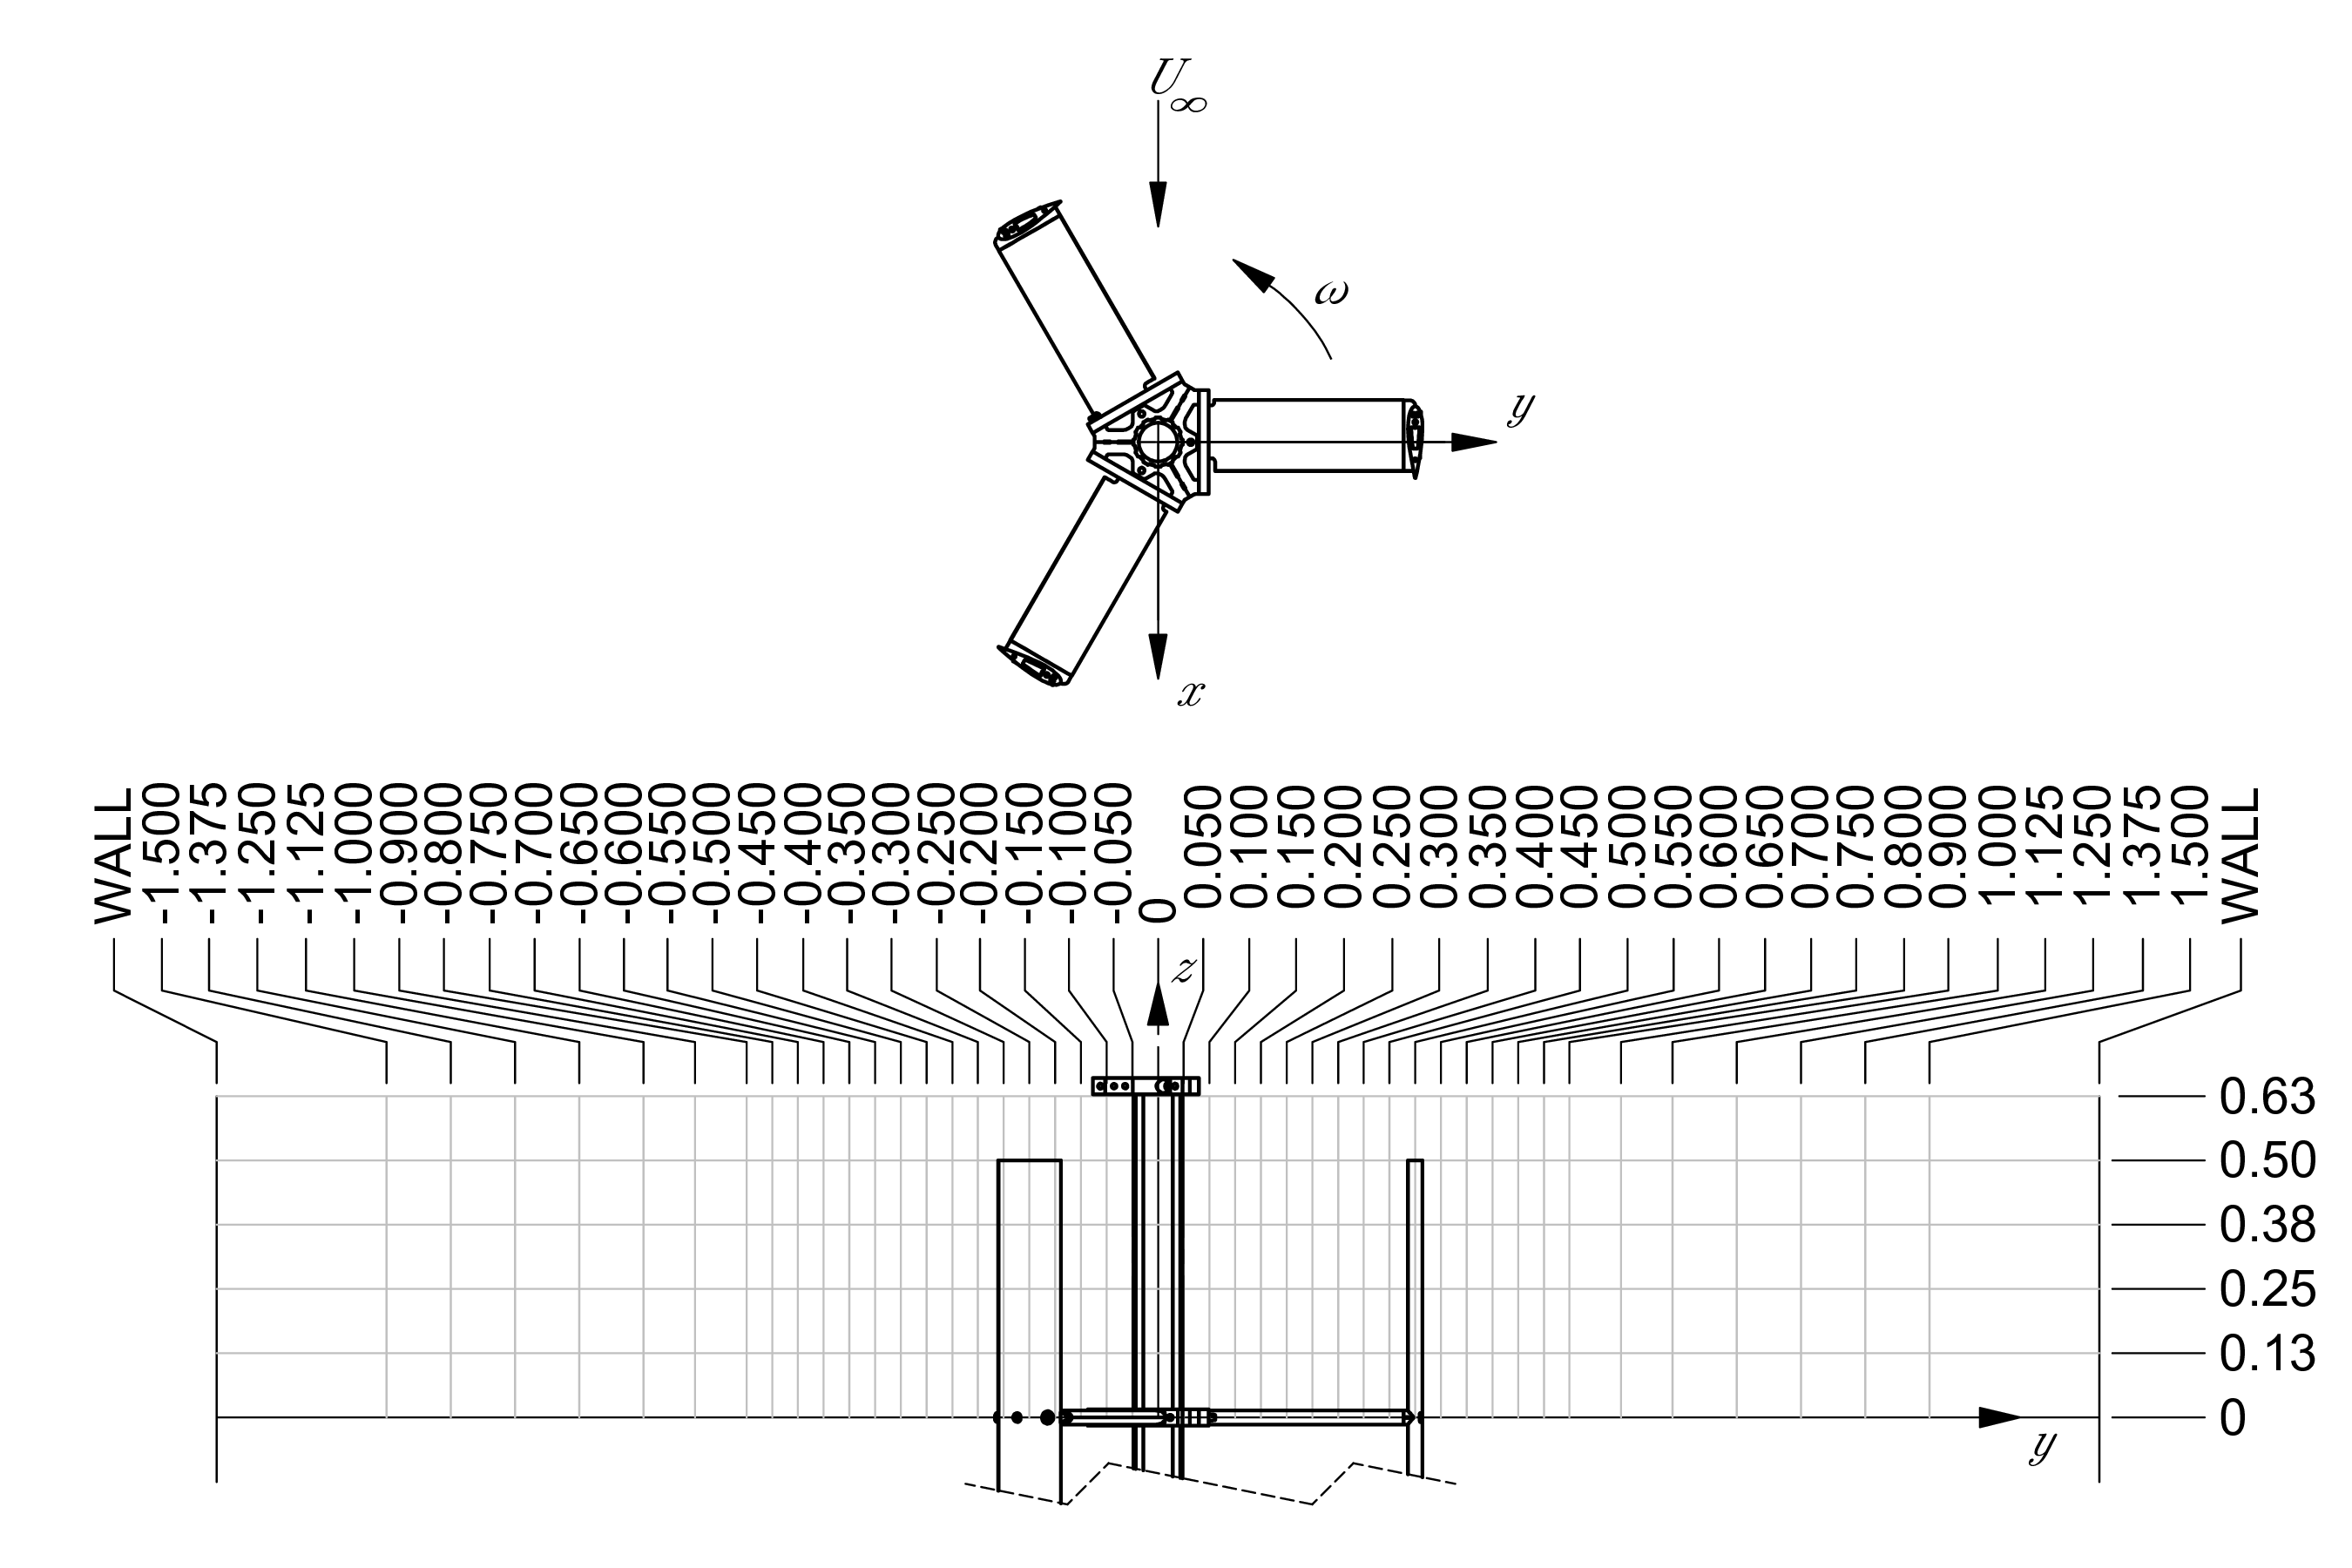
\includegraphics[width=0.9\textwidth]{unh-rvat-coord-sys}

    \caption{Wake measurement coordinate system and locations. Dimensions are in
        meters.}

    \label{fig:wake-locations}
\end{figure}


\subsection{Data processing}

From each set of tows, a standard time interval was set, which allowed the
turbine performance and wake to reach a quasi-periodic state. Each run was
analyzed to compute statistics over this interval, truncating the end slightly
to achieve an integer number of blade passages. Turbine shaft angular velocity
and tow carriage speed were calculated using a second order central differencing
scheme on the respective position measurements. Power and drag coefficients were
calculated as instantaneous quantities using the carriage speed as the free
stream velocity.

Wake velocity data were filtered for spurious ``spikes'' by removing data points
8 standard deviations, or 0.9 m/s, from the mean. The experimental data and code
for processing and visualization are available from
\cite{Bachant2016-RVAT-Re-dep}.


\subsection{Uncertainty}

Uncertainties from systematic and random error were estimated and combined using
the methods outlined in Section~\ref{sec:uncertainty}. For the Reynolds number
dependence of turbine performance, error bars are included on the plots.
Expanded uncertainty estimates for mean wake velocities (averaged over all runs)
are listed in Table~\ref{tab:vel-unc}.

\begin{table}[ht]
\centering
\begin{tabular}{c|c|c|c}
    $U_\infty$ (m/s) &   $U$ (m/s) &  $V$ (m/s) &  $W$ (m/s) \\
    \hline
    $0.4$ & $1 \times 10^{-2}$ & $7 \times 10^{-3}$ & $6 \times 10^{-3}$ \\
    $0.6$ & $1 \times 10^{-2}$ & $8 \times 10^{-3}$ & $8 \times 10^{-3}$ \\
    $0.8$ & $2 \times 10^{-2}$ & $1 \times 10^{-2}$ & $1 \times 10^{-2}$ \\
    $1.0$ & $2 \times 10^{-2}$ & $1 \times 10^{-2}$ & $1 \times 10^{-2}$ \\
    $1.2$ & $2 \times 10^{-2}$ & $1 \times 10^{-2}$ & $1 \times 10^{-2}$ \\
\end{tabular}
\caption{Average expanded uncertainty estimates (with 95\% confidence) for mean
    velocity measurements at each tow speed.}

\label{tab:vel-unc}
\end{table}


\section{Results and discussion}

\subsection{Performance}

Complete power and rotor drag (also known as thrust) coefficient curves for
various Reynolds numbers are plotted in Figures~\ref{fig:cp-curves} and
\ref{fig:cd-curves}, respectively. In general, maximum $C_P$ increases with
Reynolds number. The power coefficient curves also show a slight downward shift
in the optimal tip speed ratio (peak~performance) with increasing Reynolds
number, from about $\lambda \approx$ 2.0 to 1.9. This is caused by the stall
delay from a more turbulent boundary layer on the blade suction side. There is
essentially no change in the shape of the drag coefficient curves, merely a
slight upward shift in $C_D$ with increasing~ $Re$.

\begin{figure}
    \centering
    
    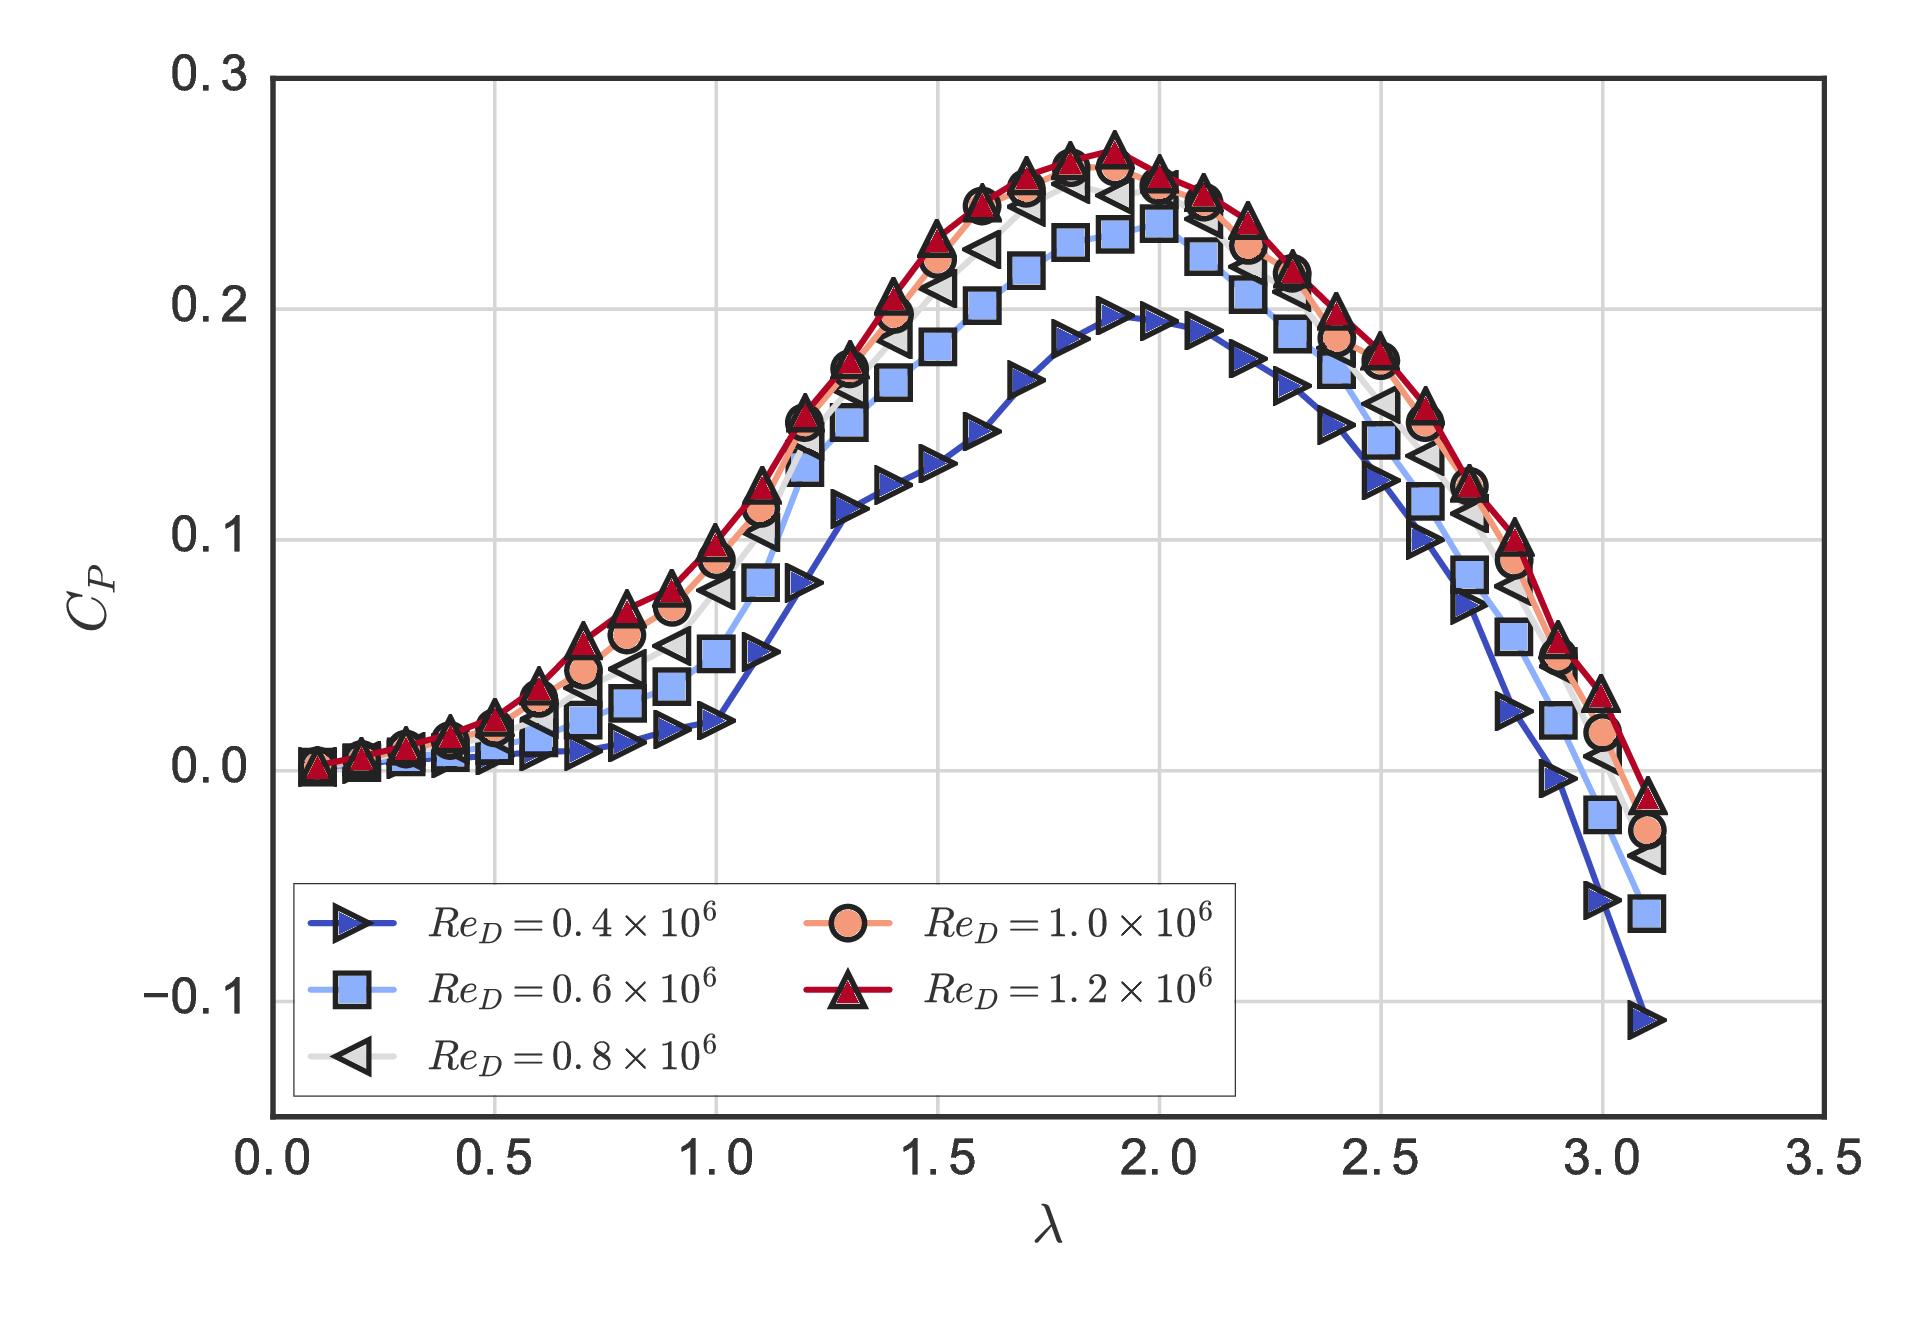
\includegraphics[width=0.75\textwidth]{RVAT-Re-dep_cp_curves}
    
    \caption{Mean power coefficient curves plotted for multiple Reynolds numbers.}
    
    \label{fig:cp-curves}
\end{figure}

\begin{figure}
    \centering
    
    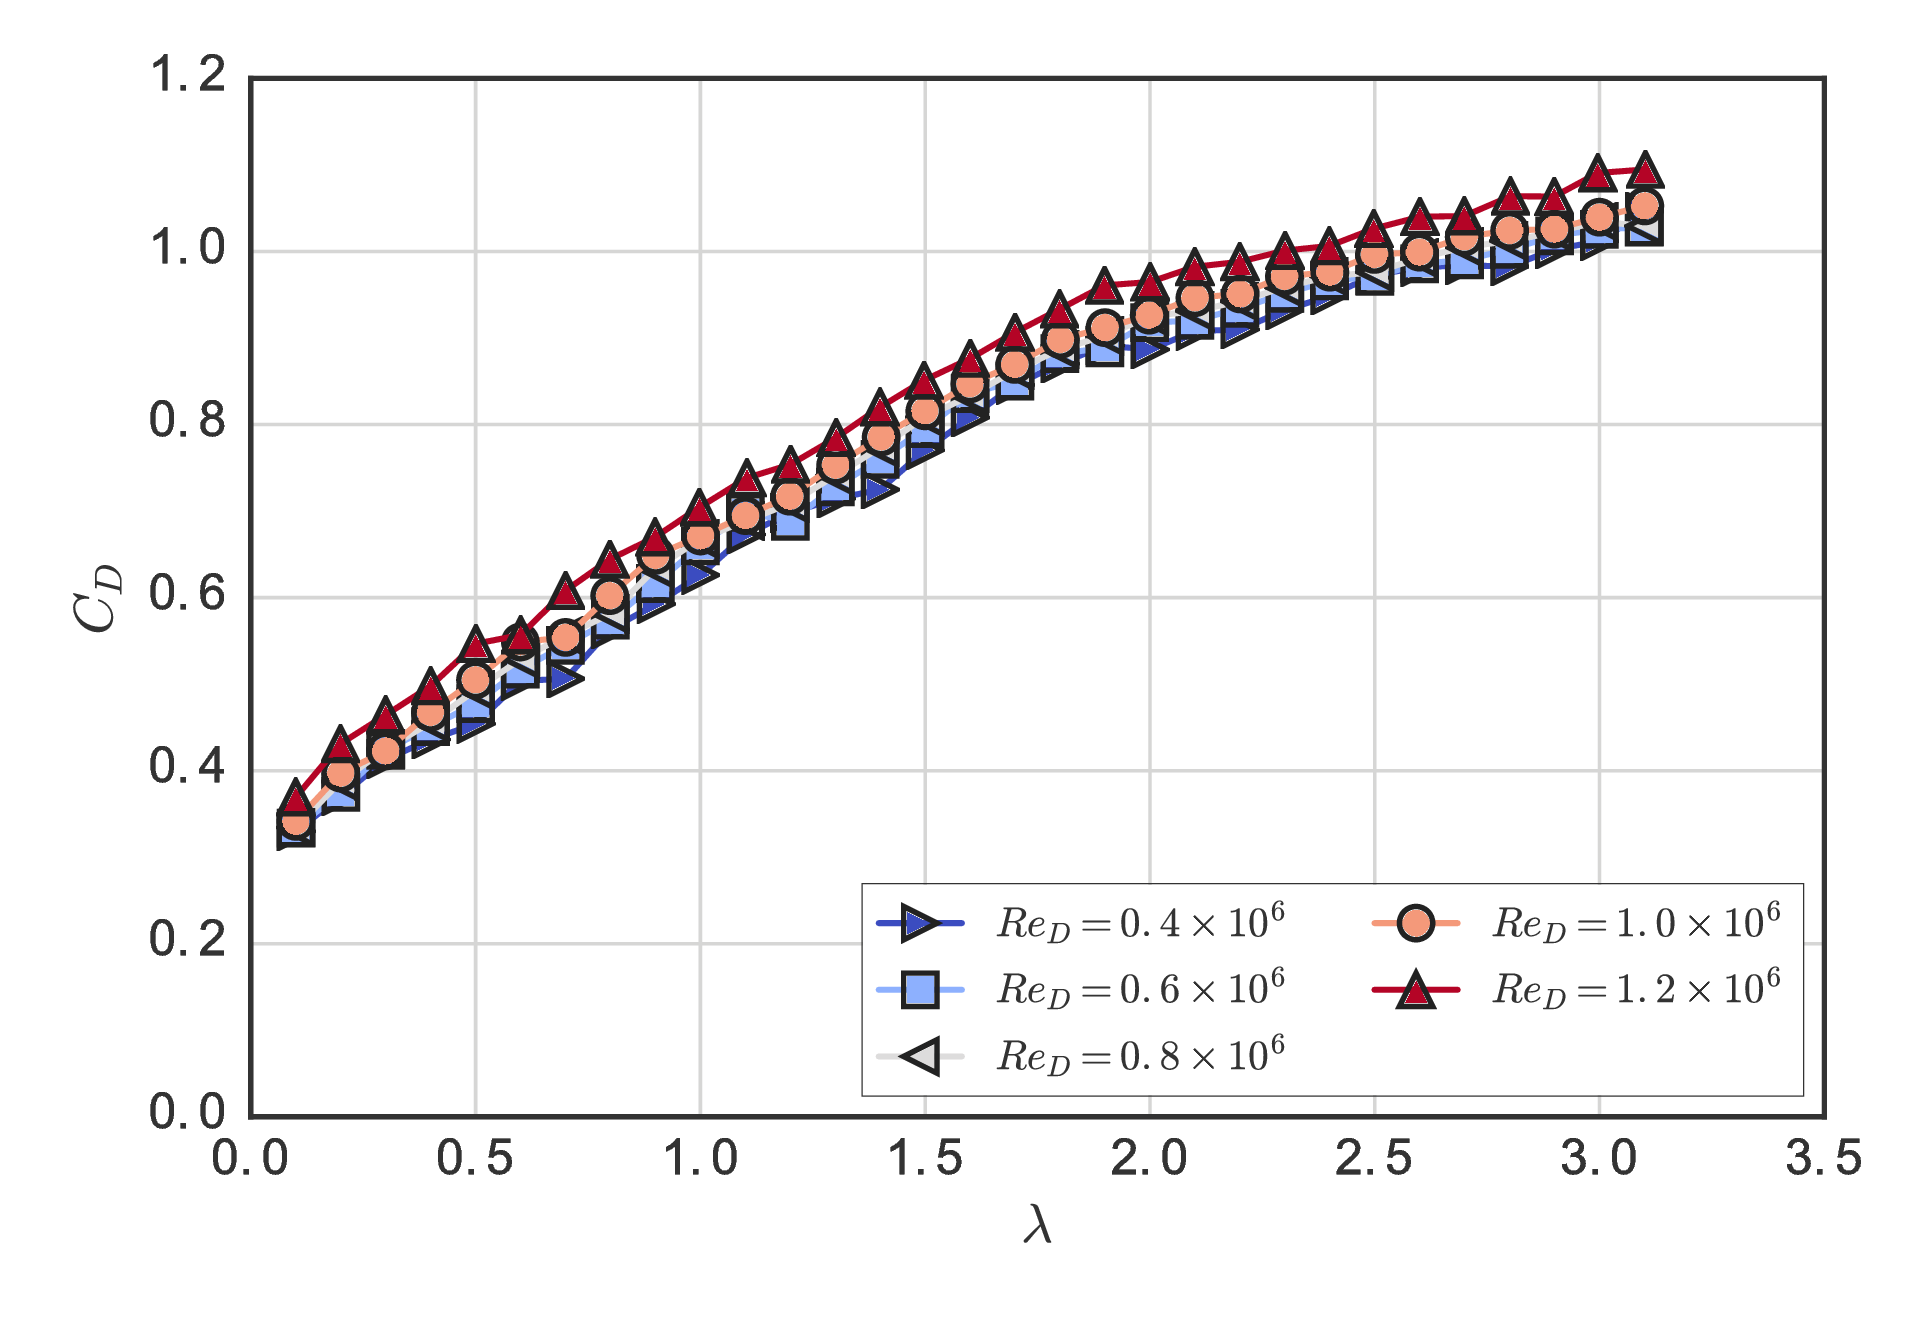
\includegraphics[width=0.75\textwidth]{RVAT-Re-dep_cd_curves}
    
    \caption{Mean rotor drag coefficient curves plotted for multiple Reynolds
        numbers.}
    
    \label{fig:cd-curves}
\end{figure}

Mean power and drag coefficients at $\lambda=1.9$ are plotted versus the
Reynolds number in Figure~\ref{fig:perf-Re-dep}. Note that the large error bars
for $C_P$ at low $Re$ are dominated by systematic error estimates for the torque
transducer, since torque values are at the lower end of its measurement range.
However, the uncertainty due to random error or repeatability remains relatively
low. There is a drastic improvement in $C_P$ with increasing Reynolds number at
the lower end of the $Re$ range. The power coefficient then becomes essentially
$Re$-independent at $Re_D = 0.8 \times 10^6$, which corresponds to an
approximate average blade chord Reynolds number $Re_{c, \mathrm{ave}} = 2.1
\times 10^5$. This threshold is consistent with the behavior of the blade
boundary layer transitioning from laminar to turbulent, thereby promoting either
the suppression or reattachment of the laminar separation bubble
\cite{Lissaman1983}.


\begin{figure}
    \centering
    
    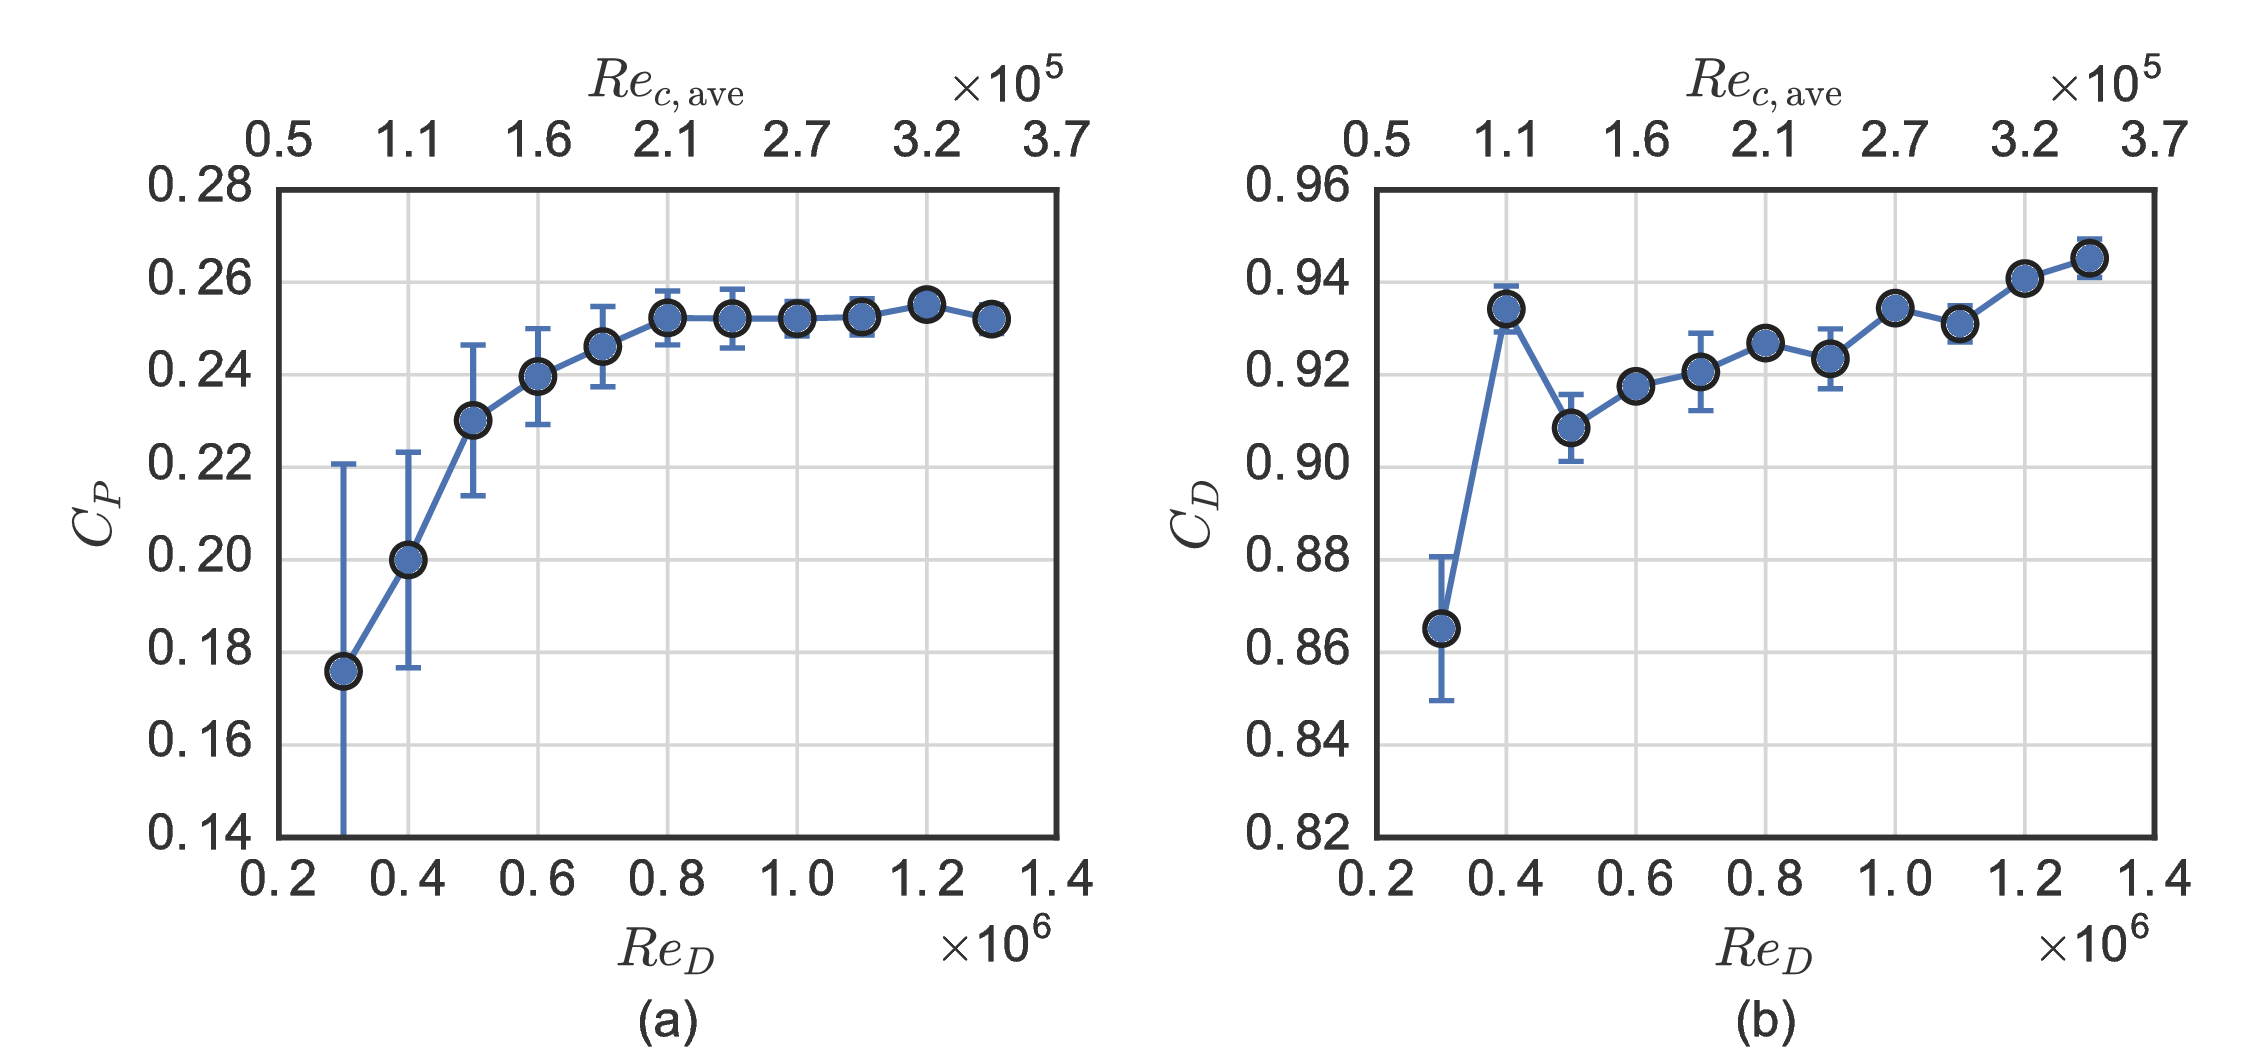
\includegraphics[width=0.9\textwidth]{RVAT-Re-dep_perf_re_dep}
    
    \caption{UNH-RVAT measured mean (a) power and (b) drag coefficients at
        $\lambda=1.9$ plotted versus the Reynolds number. Error bars indicate
        expanded uncertainty estimates for 95\% confidence, which for $C_P$ is dominated
        by systematic error estimates from the torque transducer operating at the lower
        end of its measurement range.}
    
    \label{fig:perf-Re-dep}
\end{figure}

The behavior of the mean rotor drag coefficient $C_D$ is similar, though the
changes are less dramatic. This is likely due to cross-flow turbine geometry,
where increases in blade drag at lower $Re$ somewhat offset the reduction in
lift, causing the total streamwise force to vary less than the rotor torque.
The tendency for $C_D$ to continue increasing with $Re$ may also include the
effects of an increasing Froude number (from faster tow speeds), which increases
free surface deformation and wave drag during towing without increasing flow
through the turbine.


\subsubsection{Relation to static foil characteristics}

To help understand, and possibly predict, the $Re$-sensitivity on turbine
performance, a series of static foil coefficient datasets were computed with the
viscous panel method code XFOIL \cite{Drela1989}, a commonly-used tool for
airfoil analysis, e.g., \cite{Castelli2011, Walker2014}, implemented as part of
the open source turbine design software QBlade \cite{Marten2013}. Simulations
were run for an angle of attack range of 0$^{\circ}$ to 40$^{\circ}$, in
increments of 0.5$^{\circ}$. Solver parameters used were 100 panels, a fixed
speed, zero Mach number, \texttt{NCrit=9} (default $\mathrm{e}^n$ transition
criteria parameter for an average wind tunnel), and no forced boundary layer
transition. Characteristics were computed for the approximate average blade
chord Reynolds numbers encountered in the tow tank experiments.

To investigate the effects of the blades' ``virtual camber'' due to their
circular path \cite{Migliore1980}, the XFOIL calculations were performed for
20\% thick foils with 0\% (NACA 0020), 2\% (NACA 2520), and 4\% (NACA 4520)
camber about their half-chord location. A 4\% camber approximates the maximum
distance between the blade chord line and path for the UNH-RVAT, and the 2\%
camber takes into account the reduction in virtual flow curvature from the
non-curved inflow velocity by dividing by the tip speed ratio $\lambda=1.9$.

Results from the XFOIL calculations for the airfoil profiles are shown in
Figure~\ref{fig:foil-Re-dep}, where values of the maximum lift coefficient
$C_{l_{\max}}$, minimum drag coefficient $C_{d_{\min}}$, and maximum
lift-to-drag ratio are normalized (to visualize relative differences in scaling
between the foils) and plotted versus $Re_c$. In general, larger camber
is associated with decreased foil performance at lower Reynolds number. The data
and processing code for these calculations is available from
\cite{Bachant2016-NACAXX20-XFOIL}.

\begin{figure}
    \centering
    
    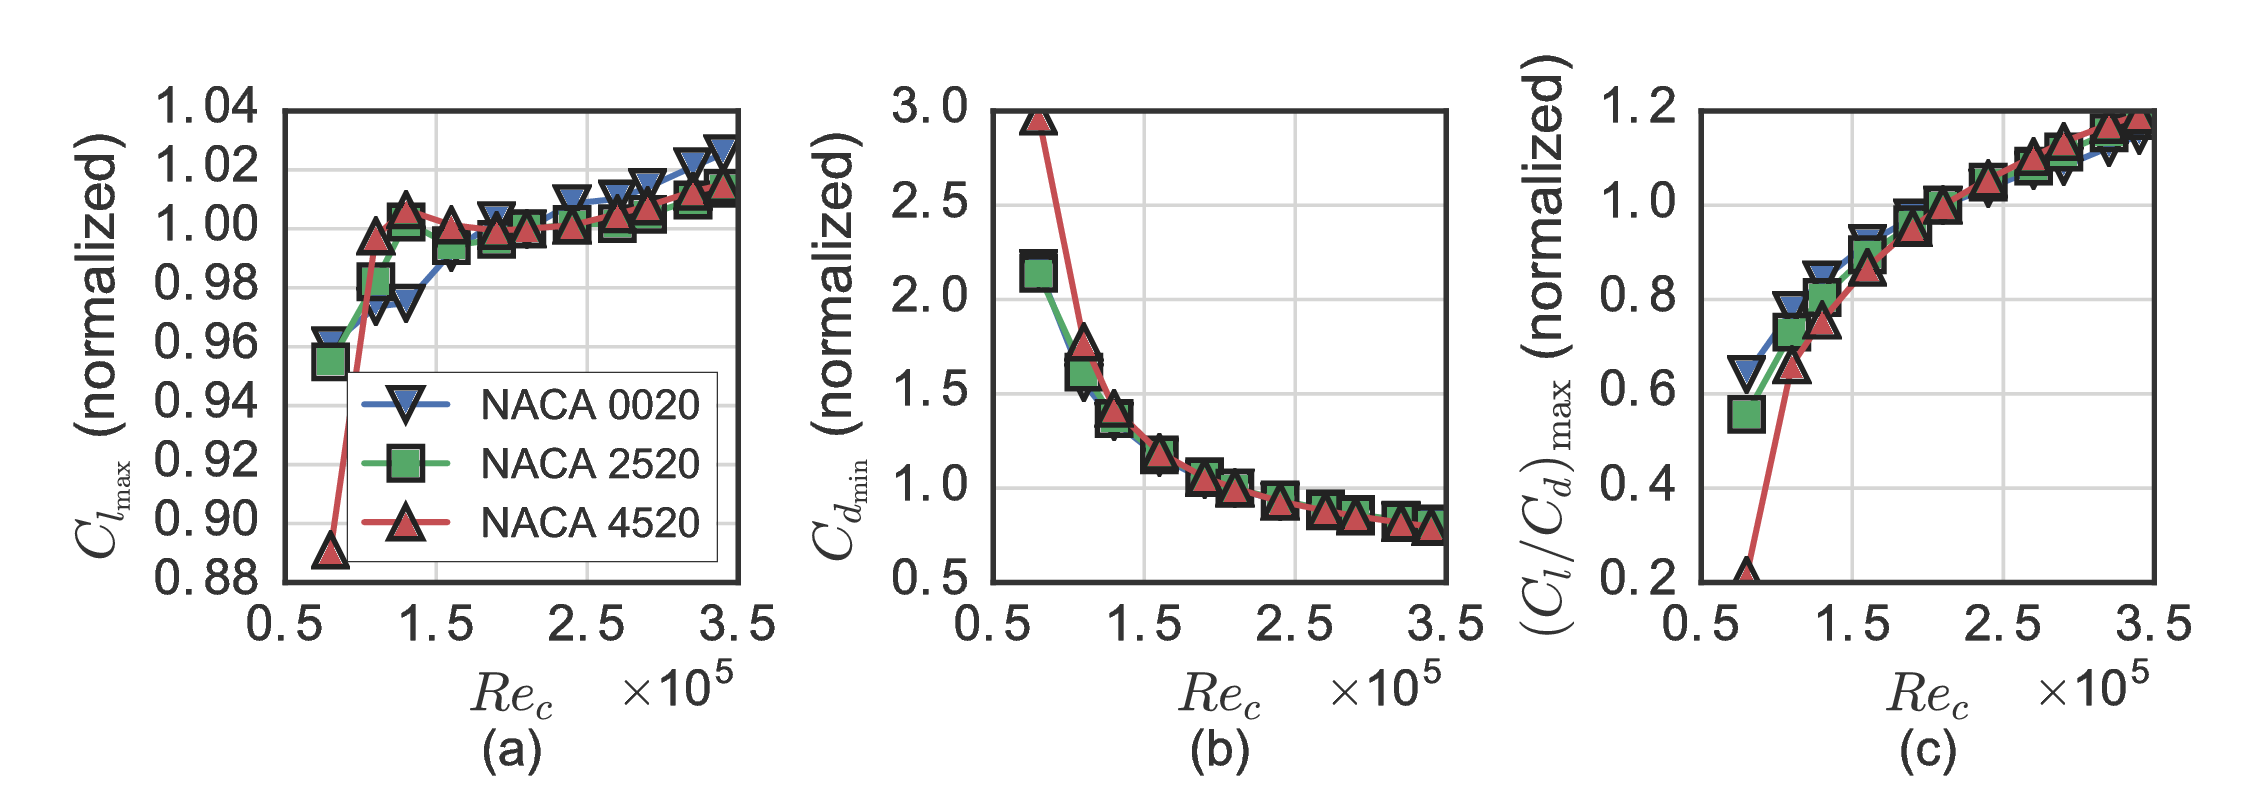
\includegraphics[width=0.95\textwidth]{NACAXX20-XFOIL_all_foils_re_dep}
    
    \caption{Normalized maximum (a) lift coefficient, (b) drag coefficient, and
        (c) lift-to-drag ratio computed by XFOIL at various $Re_c$  for each
        profile.}
    
    \label{fig:foil-Re-dep}
\end{figure}

In conjunction with the cross-flow turbine blade kinematics, the foil
coefficients were used to approximate turbine performance by calculating the
peak torque coefficient on the upstream half of the blade path. The turbine
torque coefficient $C_T$ can be related to the blade section chordwise force
coefficient $C_c$ by:
\begin{equation}
    C_T = \frac{C_c c}{2R} \frac{|U_\mathrm{rel}|^2}{U_\infty^2},
    \label{eq:ct}
\end{equation}
where the blade section chordwise force coefficient (for zero preset pitch) is
given by:
\begin{equation}
    C_c = C_l \sin \alpha - C_d \cos \alpha.
    \label{eq:cc}
\end{equation}

The relative blade velocity $U_\mathrm{rel}$ was calculated by vector addition
of the free stream velocity and the opposite of the blade tangential velocity.
Note that this neglects any induction, \emph{i.e.}, slowing of the free stream
by the turbine forces, which would be present in a momentum/streamtube model.
Since~the goal of this approach was not to predict absolute performance, but
rather to gain insight into relative changes with $Re$, this method was deemed
acceptable, as it is extremely simple and fast to~compute.

Values for the blade angle of attack, relative velocity, and torque coefficient
are plotted in Figure~\ref{fig:blade-kinematics} for the upstream half of
rotation of the turbine. The effects of static stall are clearly present in the
torque coefficient plot, and by the time the angle of attack has decreased below
the static stall angle, the relative velocity is so low that there is not much
contribution to the torque coefficient.

\begin{figure}
    \centering
    
    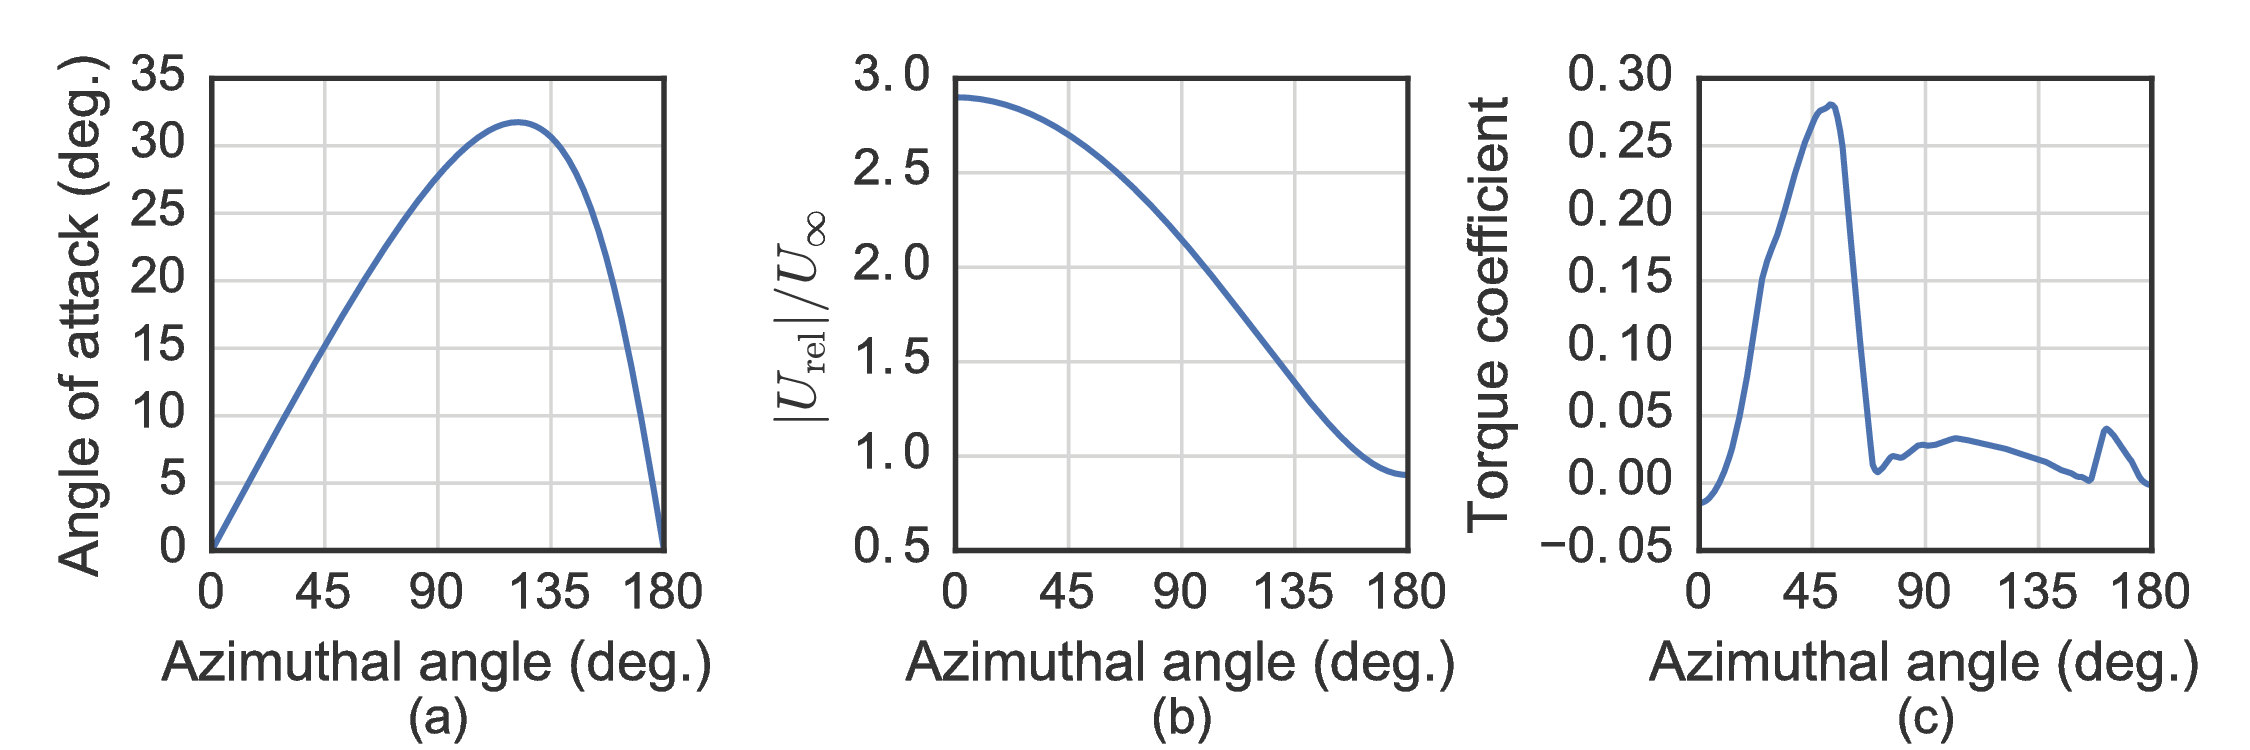
\includegraphics[width=0.95\textwidth]{NACAXX20-XFOIL_foil_kinematics_ct}
    
    \caption{Geometric (a) angle of attack, (b) relative velocity , and (c)
        torque coefficient calculated with a NACA 0020 foil operating at
        $\lambda=1.9$.}
    
    \label{fig:blade-kinematics}
\end{figure}

Results for the normalized peak torque coefficient for each foil are plotted
versus $Re_c$ in Figure~\ref{fig:foils-C_T-Re-dep}. It is interesting
that the convergence of $C_{T_\mathrm{max}}$ with increasing Reynolds number is
more dramatic than any of the common foil performance characteristics plotted in
Figure~\ref{fig:foil-Re-dep}, meaning that the cross-flow turbine's unique
kinematics must be taken into account when attempting to predict the effect of
transitional Reynolds numbers on turbine performance.

From the peak torque coefficient metric plotted in
Figure~\ref{fig:foils-C_T-Re-dep}, the Reynolds number independence is achieved
at lower values and more dramatically. We see that the trend of the
(non-cambered) NACA 0020 curve matches almost perfectly up to $Re_c \approx 2.1
\times 10^5$, but then continues to increase slowly and linearly with $Re$. This
is not matched by the experimental data, which at higher $Re$ looks more like
the cambered foil results. Though this method does not provide absolute
predictions of turbine performance, it predicts the transitional Reynolds number
regime for cross-flow turbine performance using only 2D static airfoil
characteristics, \emph{i.e.}, the Reynolds number scaling of the peak $C_T$
computed this way behaves much like that of the measured turbine performance.

\begin{figure}
    \centering
    
    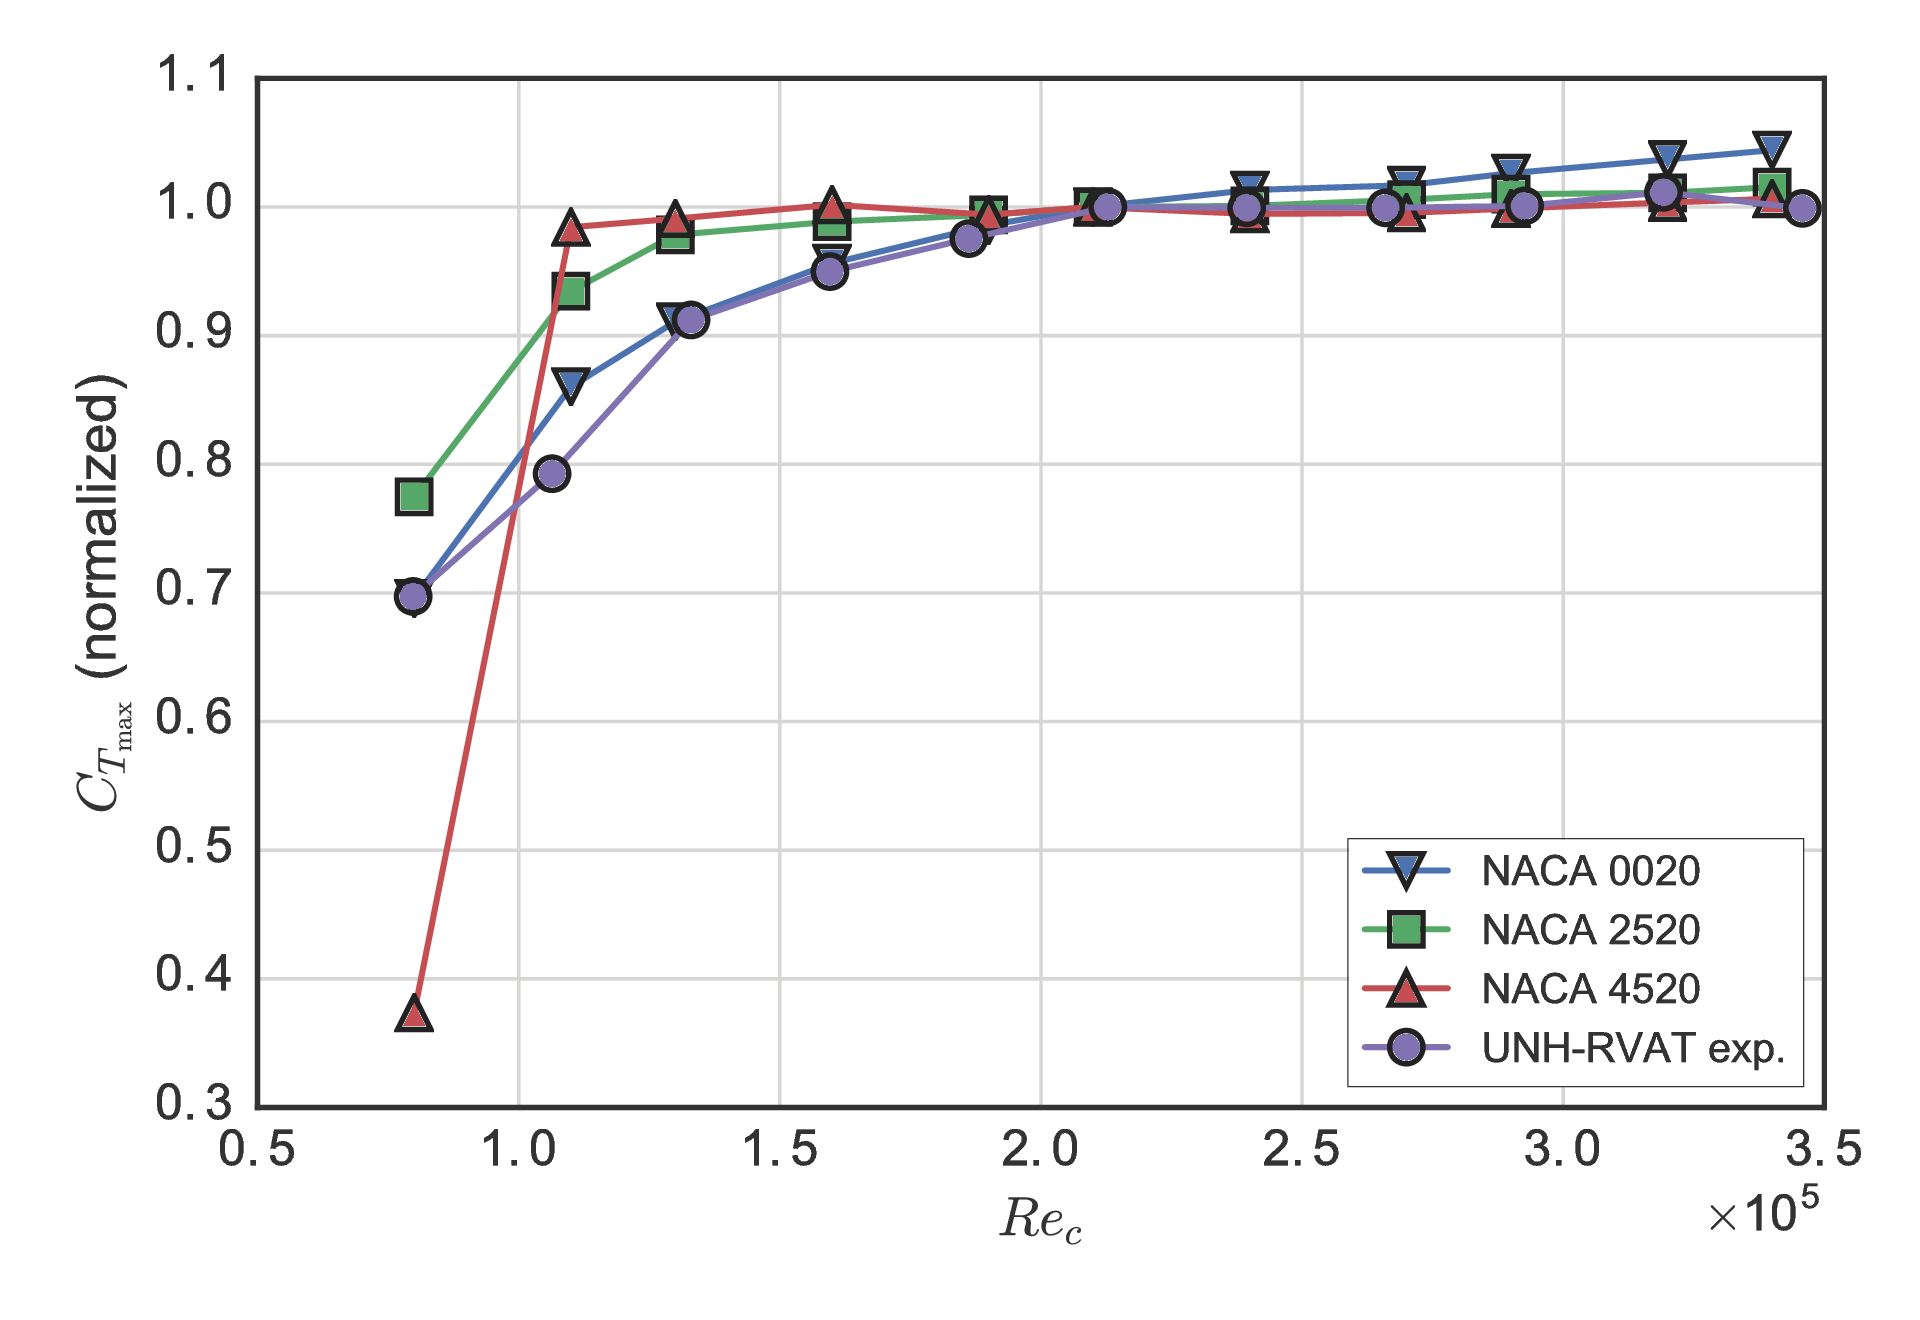
\includegraphics[width=0.75\textwidth]{NACAXX20-XFOIL_cft_re_dep_foils}
    
    \caption{Reynolds number dependence of the normalized peak torque
        coefficient calculated from static foil coefficients and blade kinematics,
        compared to experimental data from a cross-flow turbine. Note that the
        experimental data represents the mean torque coefficient, not the maximum.}
    
    \label{fig:foils-C_T-Re-dep}
\end{figure}


\subsection{Wake characteristics}

The near-wake of this turbine at $x/D=1$, $\lambda=1.9$, along with momentum and
kinetic energy balances at a $Re_D = 1.0 \times 10^6$ were discussed in
\cite{Bachant2015-JoT}. Similar data were taken for the experiment here, and the
results for the mean velocity field and turbulence kinetic energy calculated
from wake maps of 270 individual measurements (tows) are shown in
Figures~\ref{fig:meancontquiv} and \ref{fig:kcont}, respectively, looking
upstream towards the turbine. With respect to the mean velocity field, we see
asymmetry and a mean vortex structure created by blade tip vortex shedding. The
effects of the tip vortices are also seen in the turbulence kinetic energy
measurements, along with turbulence generated by the blades undergoing dynamic
stall on the $-y$ side of the turbine.

These same wake maps were measured for $Re_D = 0.4 \times 10^6$, $0.6 \times
10^6$, $0.8 \times 10^6$, and $1.2 \times 10^6$. Qualitatively, these look very
similar, so they have not been plotted here, though profiles at $z/H=0.0$ are
compared in Figure~\ref{fig:profiles} to illustrate the subtlety of the
differences at different $Re$. We will instead compare and contrast the wake
behavior by examining spectra and wake transport terms in the equations that
govern the downstream evolution of mean momentum and kinetic energy.

\begin{figure}
    \centering
    
    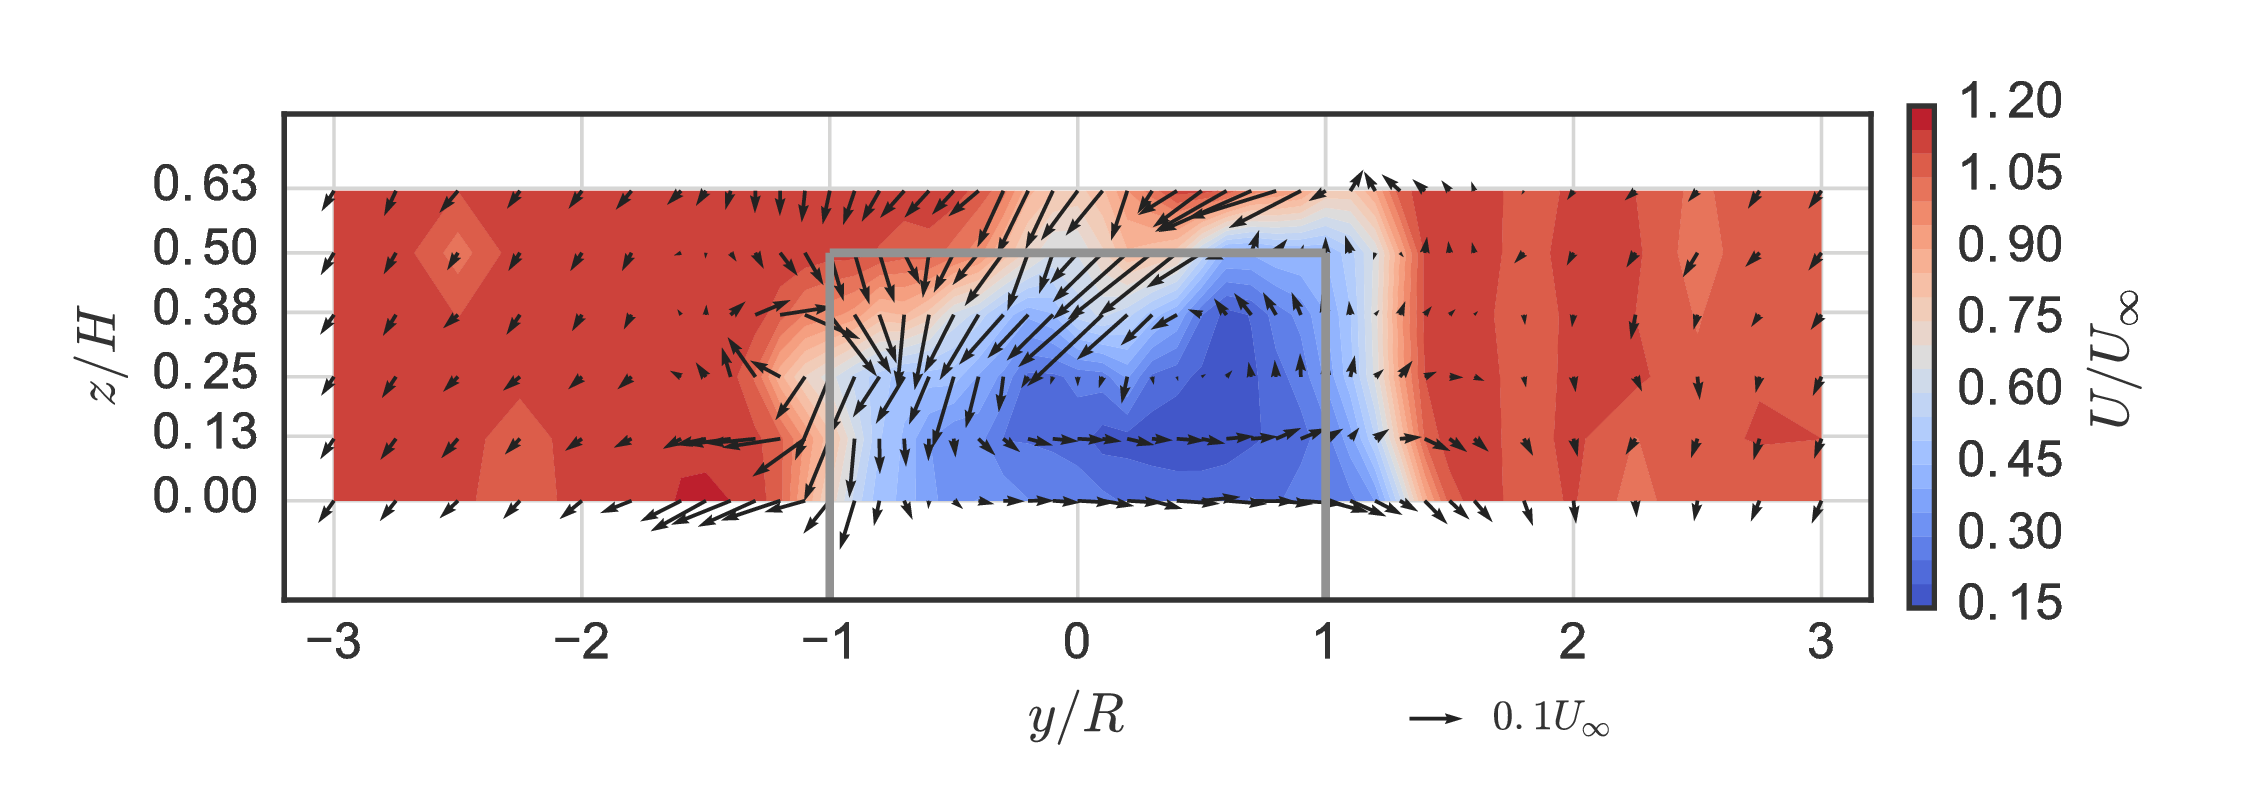
\includegraphics[width=0.85\textwidth]{RVAT-Re-dep_meancontquiv_10}
    
    \caption{Mean velocity field at $x/D=1$, $\lambda=1.9$, and $Re_D=1.0 \times
        10^6$.}
    
    \label{fig:meancontquiv}
\end{figure}

\begin{figure}
    \centering
    
    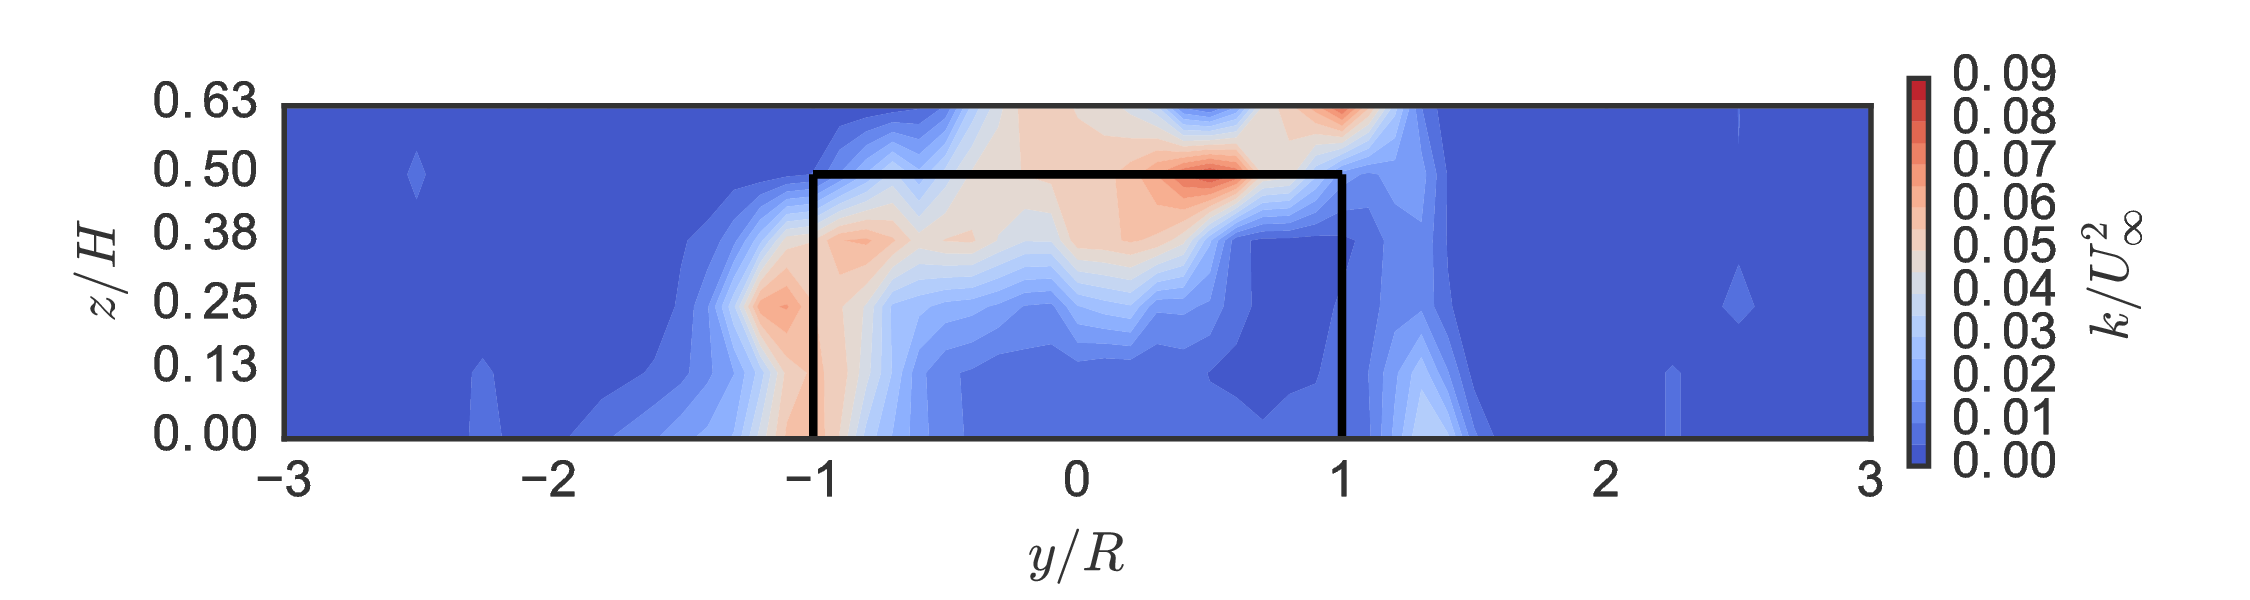
\includegraphics[width=0.85\textwidth]{RVAT-Re-dep_k_contours_10}
    
    \caption{Turbulence kinetic energy at $x/D=1$, $\lambda=1.9$, and $Re_D=1.0
        \times 10^6$.}
    
    \label{fig:kcont}
\end{figure}

\begin{figure}[ht]
    \centering
    
    \includegraphics[width=0.9\textwidth]{RVAT-Re-dep_mean_u_k_profiles}
    
    \caption{Mean streamwise velocity (a) and turbulence kinetic energy (b)
        profiles at $z/H=0.0$. Turbine diameter Reynolds number $Re_D$ is indicated
        by the legend.}
    
    \label{fig:profiles}
\end{figure}

\todo[inline]{Profiles fig should have legend in lower left.}


\subsubsection{Dominant timescales and turbulence spectra}

Spectra of the cross-stream velocity normalized by the free stream were computed
using a fast Fourier transform-based method, applying a Hanning window and
averaging over four adjacent frequency bands to decrease confidence intervals.
These spectra are plotted in Figure~\ref{fig:wake-spectra} for regions on either
side of the turbine. On the $-y$ side of the turbine, there is broadband
turbulence produced by blade stall, and on the $+y$ side, there is a clear peak
in the spectra caused by the blade passage. We see that on both sides, there is
higher spectral energy at lower Reynolds numbers. On the $+y$ side of the
turbine, we notice higher spectral energy at the blade passage frequency's first
harmonic, or $6 f_\mathrm{turbine}$. This is likely due to the blade's shed
vorticity being less stable at higher $Re$.

\begin{figure}
    \centering
    
    \includegraphics[width=0.85\textwidth]{RVAT-Re-dep_wake_spectra}
    
    \caption{Cross-stream velocity (normalized by $U_\infty$) spectra at
        $z/H=0.25$, $y/R=-1.0$ ($-0.5$ m in Figure~\ref{fig:wake-locations}) (a) and
        $y/R=1.5$ ($+0.75$ m in Figure~\ref{fig:wake-locations}) (b). Dashed
        vertical lines indicate $[1, 3, 6, 9]$ times the turbine rotational
        frequency. Shaded regions indicate 95\% confidence intervals assuming a
        $\chi^2$~distribution.}
    
    \label{fig:wake-spectra}
\end{figure}


\subsubsection{Transport of mean momentum and kinetic energy}

Similar to the baseline analysis performed in Chapter~\ref{chap:RVAT-baseline},
the relative importance of various physical processes on mean streamwise
momentum and kinetic energy transport/recovery in the streamwise direction were
assessed at each Reynolds numbers. The governing equations were rearranged to
isolate the streamwise partial derivative ($\partial / \partial x$) for the
quantities of interest~\cite{Bachant2015-JoT}, i.e., streamwise momentum and
mean kinetic energy.

Results from the terms that can be computed from the experimental data i.e.,
excluding $\partial / \partial x$) from the right-hand sides of
Equations~(\ref{eq:momentum}) and (\ref{eq:K-full}) are plotted in
Figures~\ref{fig:mom-bar-graph} and \ref{fig:K-bar-graph}, respectively.
Derivatives were computed using a second order finite difference scheme, with
central differencing for interior points and inward facing schemes for the
boundaries. A weighted average for each term was then calculated based on the
grid spacing. We note that similar to \cite{Bachant2015-JoT}, the vertical
advection at this point in the wake is the dominant contributor to positive wake
recovery, caused by the unique vortex pattern created by the blade tips and
blade wakes.

\begin{figure}
    \centering
    
    \includegraphics[width=0.9\textwidth]{RVAT-Re-dep_mom_bar_graph}
    
    \caption{Normalized streamwise momentum transport quantities computed as
        weighted averages from Equation~\ref{eq:momentum}.}
    
    \label{fig:mom-bar-graph}
\end{figure}

\begin{figure}
    \centering
    
    \includegraphics[width=0.9\textwidth]{RVAT-Re-dep_K_trans_bar_graph}
    
    \caption{Normalized mean kinetic energy transport quantities computed as
        weighted averages based on Equation~(\ref{eq:K-full}), omitting the
        non-measured streamwise derivatives. Note that directions of the turbulent
        transport terms refer to the directions of their partial derivatives.}
    
    \label{fig:K-bar-graph}
\end{figure}

We see that in general, levels of turbulent transport are slightly lower at
larger Reynolds numbers. The viscous diffusion and dissipation, though still
three orders of magnitude smaller than the other terms, do increase at low
Reynolds numbers, which is consistent with the physical meaning of the Reynolds
number itself. From these results, one might expect that the viscous effects
will become significant to the wake dynamics as the Reynolds number is decreased
below $Re_D \sim 10^4$.

Transport due to cross-stream advection appears to become more negative at
higher $Re$. This~could be a consequence of increasing free surface deformation
(higher $Fr$), which then decreases the effective flow cross-sectional area
downstream of the turbine, forcing more flow to accelerate around the sides of
the turbine. Note that we also observe slightly higher drag coefficients at
higher $Re$ (potentially for the same reason), which also helps explain larger
negative values of cross-stream advection.

The totals for all of the wake transport terms calculated in
Figures~\ref{fig:mom-bar-graph} and \ref{fig:K-bar-graph} are plotted in
Figure~\ref{fig:RVAT-Re-dep-wake-trans-totals}. We see that in general, the wake
transport of both mean streamwise momentum and kinetic energy is enhanced at
lower Reynolds numbers and levels off consistent with the behavior of the
turbine power coefficient. This is an important consideration if studying
sub-scale models of turbine arrays, where increased levels of wake recovery
could motivate different ideal array configurations when compared to full-scale
turbines if the scale model Reynolds number is too low.

\begin{figure}
    \centering
    
    \includegraphics[width=0.75\textwidth]{RVAT-Re-dep_wake_trans_totals}
    
    \caption{Normalized transport totals from Figures~\ref{fig:mom-bar-graph}
        (streamwise momentum, $U$) and \ref{fig:K-bar-graph} (mean kinetic energy,
        $K$) plotted versus the Reynolds number.}
    
    \label{fig:RVAT-Re-dep-wake-trans-totals}
\end{figure}

\todo[inline]{Make labels more specific.}


\section{Conclusions}

In this study, it was demonstrated that the performance of a high solidity
($c/R=0.28$) cross-flow turbine becomes essentially $Re$-independent at a
Reynolds number based on the turbine diameter $Re_D \approx 10^6$ or an
approximate Reynolds number based on the blade chord $Re_c \approx 2 \times
10^5$. The power coefficient values on the left-hand side of the $C_P$-$\lambda$
curve are reduced more than those on the right-hand side at low $Re$ due to
deeper stalling. The $Re$-independent threshold corresponds to that at which the
foil suction surface boundary layer becomes turbulent before having to recover
static pressure against the adverse pressure gradient, highlighted in
\cite{Lissaman1983, McMasters1980, Carmichael1981}.

We propose a method for predicting the Reynolds number dependence of a cross-flow
turbine using static airfoil characteristics and turbine blade kinematics:
\begin{enumerate}
    \item Acquire static lift and drag coefficient data for the desired blade
    profile.
    
    \item For azimuthal angles of 0 to 180 degrees and a given tip speed ratio,
    calculate the geometric angle of attack and relative velocity magnitude from
    the blade and undisturbed free stream velocity (taken as unity) vectors.
    
    \item With arrays of geometric angle of attack and relative velocity
    magnitude, calculate the blade chordwise force and then the rotor torque
    coefficient from Equations~(\ref{eq:ct}) and (\ref{eq:cc}), respectively.
    
    \item Extract the maximum value of $C_T$, and repeat this process for static
    foil data at multiple $Re$.
\end{enumerate}

It was shown that the peak torque coefficient computed this way shows similar
Reynolds number sensitivity as the experimental results for an actual turbine,
making it a better predictor than conventional quantifications of airfoil
performance, e.g., the lift-to-drag ratio. Note that this method is not
restricted to standard symmetrical NACA foils, though those evaluated here with
higher camber were more sensitive at lower $Re$, but had smaller slopes in the
linear~regime.

In the near-wake of the turbine, we observed lower levels of turbulence with
increasing Reynolds number, along with lower levels of turbulent transport with
respect to mean streamwise momentum and mean kinetic energy recovery in the
streamwise direction. Vertical advection, the largest transport mechanism
measured, showed little $Re$-dependence, whereas the negative effects of
cross-stream advection were enhanced at high $Re$, which may be due to larger
free surface deformation effectively reducing the near-wake's cross-sectional
area. Despite being orders of magnitude smaller than other transport processes,
viscous diffusion increased rapidly with decreasing $Re$ and is expected to
become significant to the wake dynamics around $Re_D \sim 10^4$. Overall, the
total wake transport measured leveled off at essentially the same Reynolds
number that the performance did: $Re_D \approx 0.8 \times 10^6$.

From these results, we recommend that physical model tests of cross-flow
turbines be performed at $Re_D \sim 10^6$ or greater to provide reasonable
predictions of full-scale performance. This threshold also applies to the
validation of predictive engineering models, especially for high-fidelity CFD
models where the boundary layer is to be resolved, since transition to
turbulence plays an important role in overall blade loading. Note that in our
case, blockage, though reasonably low, may be increasing flow through the
turbine compared to a free case, which could mean $Re$ thresholds for free flows
could be slightly higher, though a reliable blockage correction algorithm has
not yet been agreed upon for CFTs~\cite{Cavagnaro2014}.

If using scaled physical models to predict array performance, where turbine
power output is measured, it may also be important to keep all turbines in the
regime where the power coefficient varies linearly to avoid exaggerated power
deficiencies for downstream turbines, despite similarities in wake
characteristics. Results here also suggest that low Reynolds number physical
model studies of turbine arrays may see exaggerated levels of wake recovery,
leading to inadequate or inappropriate spacing or layouts.
% Chapter on RM2 experiments, including wake, Re dep, strut drag
\chapter{Experimental characterization of a low-solidity cross-flow turbine}

For the low solidity RM2, the performance was characterized at multiple Reynolds
numbers, with the near-wake at only one, for comparing to the RVAT baseline
data.

\subsection{Turbine model}

The RM2 CFT was initially conceptualized by Sandia National Labs for the US
Department of Energy to be a generic case for numerical modeling
\cite{Barone2011}, specifically Sandia's CACTUS vortex model. With the blade and
strut parameters specified, a turbine model was designed and machined from
6061-T6 aluminum. The hub design mimicked that of the smaller scale RM2 build by
the Saint Anthony Falls Laboratory (SAFL) \cite{Hill2014}, though the blade to
strut connections were more streamlined.

\section{Experimental test plan}
% Chapter on blade-resolved RANS
\chapter{On the use of blade-resolved computational fluid
    dynamics}\label{chap:CFD}

In this chapter we will evaluate the effectiveness of modern high-fidelity
computational fluid dynamics (CFD) for predicting the performance and near-wake
characteristics observed for the UNH-RVAT. The content presented here has been
submitted for publication as~\cite{Bachant2016-BR-CFD}.

Despite the development of many simple engineering models based on blade element
momentum or vortex methods, it remains difficult to predict the performance of
cross-flow turbines (CFTs, often vertical-axis turbines or VATs) for all
cases---namely when solidity, or blade chord-to-radius ratio is high---a common
characteristic of smaller rotors, and those designed for marine hydrokinetic
(MHK) applications. With computing power becoming evermore available and
affordable, CFD based on the Reynolds-averaged Navier--Stokes (RANS) equations
has become an attractive method for predicting the performance of cross-flow
turbines. Since a direct numerical simulation (DNS) of all scales at realisitc
Reynolds numbers is not currently feasible, turbulence be modeled. However, with
an appropriate turbulence model, blade-resolved RANS presents a more physically
realistic first principles based approach versus simpler models based on
momentum theory or potential flow. However, CFD can be computationally expensive
when done in three dimensions, which may be necessary in some cases.

\nomenclature{DNS}{Direct numerical simulation.}

There are many examples in the literature of 2-D cross-flow turbine simulations
with widely varying results. Balduzzi et al.~\cite{Balduzzi2016} provides
a summary of recent efforts and an attempt to standardize a methodology for
using Reynolds-averaged Navier--Stokes (RANS) to correctly predict performance
of a 2-D CFT. Howell et al.~\cite{Howell2010}, performed both 2-D and 3-D
simulations of a high solidity cross-flow turbine using a $k$--$\epsilon$
renormalization group (RNG) turbulence model. The results from the 2-D
simulations over-predicted power coefficient, while the 3-D case matched well
with wind tunnel measurements near the tip speed ratio of maximum power. In
general, 3-D simulations are less common, but have begun to appear more
frequently recently---a testament to the progress towards higher computing
power.

An overview of 3-D blade-resolved cross-flow turbine simulations reported in the
literature is presented in Table~\ref{tab:cfd-refs}. The $k$--$\omega$ SST RANS
turbulence model is shown to be a popular choice due to its success in
predicting flows with adverse pressure gradients and
separation~\cite{Menter2003}. Higher fidelity methods that resolve the large
scales of turbulence, such as large eddy and detached eddy simulation have also
been used. Note that for all the studies listed, model validation was performed
for either performance or wake predictions---not both---and in some case omitted
entirely.

\begin{table}
    \centering
    \begin{tabular}{c|c|c|c}
        Author & Turbulence modeling & Perf. val. & Wake val. \\
        \hline
        Alaimo et al.~\cite{Alaimo2015} & $k$--$\epsilon$ RANS & N/A & N/A \\
        Marsh et al.~\cite{Marsh2015} & SST RANS & \cite{Rawlings2008} & N/A \\
        Orlandi et al.~\cite{Orlandi2015} & SST RANS & \cite{Akins1989,Mertens2003} & N/A \\
        Lam \& Peng~\cite{Lam2016} & SST RANS \& IDDES\tablefootnote{Improved delayed detached eddy simulation.} & N/A & \cite{Tescione2014} \\
        Nini et al.~\cite{Nini2014} & Spalart--Allmaras RANS & N/A & \cite{Battisti2011} \\
        Boudreau \& Dumas~\cite{Boudreau2015} & Spalart--Allmaras DDES\tablefootnote{Delayed detached eddy simulation.} & N/A & N/A \\
        Li et al.~\cite{Li2013} & SST RANS \& Smagorinsky--Lilly LES & \cite{McLaren2011} & N/A \\
        Howell et al.~\cite{Howell2010} & $k$--$\epsilon$ RNG\tablefootnote{Renormalization group.} RANS & \cite{Howell2010} & N/A
    \end{tabular}

    \caption{Selected 3-D blade-resolved cross-flow turbine simulations reported
    in the literature, turbulence modeling employed, and performance and/or wake
    studies used for validation. Note the Li et al. study used periodic boundary
    conditions and is technically considered 2.5-D.}

    \label{tab:cfd-refs}
\end{table}

\nomenclature{DES}{Detached eddy simulation.}
\nomenclature{DDES}{Delayed detached eddy simulation}
\nomenclature{IDDES}{Improved delayed detached eddy simulation.}
\nomenclature{RNG}{Renormalization group.}

Modeling the boundary layer flows on cross-flow turbine blades is essential to
predicting the blade loading. This flow condition presents a challenge due to
the dynamically changing inflow velocity and angle of attack---which often
exceeds static stall values and causes dynamic stall. Furthermore, the ability
to predict the occurrence and interdependence of boundary layer transition to
turbulence and separation can have dramatic influence on the blade loading and
therefore the predicted turbine power output. These challenges present
significant obstacles to the prospect of using CFD to replace wind tunnel or
tank testing of physical models.

To date, little computational work has been done to attempt to design arrays of
CFTs, despite their prospects for closer spacing compared with axial-flow
turbines (AFTs). For example, Araya et al.~\cite{Araya2014} modeled the flow
through a VAT array using ``leaky Rankine body'' potential flow singularities,
which was able to rank relative---though not absolute---performance of array
configurations. Goude and Agren~\cite{Goude2010} used a 2-D vortex method to
simulate a farm of cross-flow turbines, though this was not validated with
experiments. Durrani et al.~\cite{Durrani2011} used 2-D CFD to model a group of
cross-flow turbines, observing higher power output for a staggered
configuration, but also did not compare with experimental results. Giorgetti et
al.~\cite{Giorgetti2015} took a similar approach for 2-D array analysis using
turbine pairs inspired by Dabiri~\cite{Dabiri2011}, but again experimental
validation was not performed. Li and Calisal \cite{Li2010} used a 3-D vortex
line method to show mutually improved power output from two adjacent turbines,
though the simulations over-predicted the effectsby approximately 5\% compared
with experiments. Antheaume et al.~\cite{Antheaume2008} used a blade element
approach coupled with a 3-D RANS solver to also show how close spacing can
improve power output of CFTs.

In this study we set out to model the performance and near-wake of the high
solidity University of New Hampshire Reference Vertical-Axis Turbine (UNH-RVAT)
using the Reynolds-averaged Navier--Stokes equations discretized via the finite
volume method. Though studies in the literature generally focus on predicting
the turbine loading and the local blade boundary layer, we seek to model both
this and the larger scale flow produced by the rotor, i.e., the near-wake, which
is of interest for this particular turbine since it has been shown
experimentally that the near-wake's momentum and energy transport processes are
dominated by vertical advection \cite{Bachant2015-JoT}. It logically follows
that a 2-D simulation, which omits the vertical dimension, would not correctly
predict wake recovery and turbine--turbine interaction. However, it is of
interest to determine how wrong a 2-D model may be, since the lower
computational cost of 2-D simulations is attractive.

We seek to validate 2-D and 3-D blade-resolved RANS models against the UNH-RVAT
mechanical power and near-wake measurements. If the blade loading and velocity
in the near-wake match well enough, the flow field can potentially be inspected
in greater detail, i.e., we may be able to make observations of quantities not
measured experimentally, e.g., pressure, and gain greater insight into where the
dominant flow structures originate. This will ultimately help develop and
evaluate low-order wake generator models for use in turbine array modeling. In
summary, the questions we hope to answer here are:

\begin{enumerate}
    \item Can 2-D RANS be used for individual turbine and/or array design?

    \item How accurately can 3-D RANS predict performance?

    \item Can 3-D RANS ``interpolate'' the experimental results and provide
    insight to develop new low-order wake generators to represent CFTs?

    \item Does 3-D RANS realize the correct proportions of wake recovery
    mechanisms, i.e., are the 3-D blade-resolved results a good ``target'' for
    those a low-order model should produce?
\end{enumerate}


\section{Numerical setup}

In this study the UNH-RVAT baseline tow tank experiment was simulated using a
mean rotor tip speed ratio $\lambda=1.9$, which corresponds to the maximum
measured power coefficient. The tow speed or free stream velocity $U_\infty=1.0$
m/s gives a turbine diameter Reynolds number $Re_D \approx 10^6$, which
corresponds to the $Re$-independent state for both performance and near-wake
characteristics, as determined from previous experimental measurements
\cite{Bachant2014, Bachant2016-Energies}.

The turbines CAD geometry was prepared or ``cleaned'' for CFD by removing
details determined to be unnecessary, e.g., screw heads and axial shaft grooves,
which would complicate the meshing process and contribute very little to the
overall loading or flow modulation. A drawing of the physically and numerically
modeled geometries is presented in Figure~\ref{fig:cfd-cad}.

\begin{figure}
    \centering

    \includegraphics[clip, trim=0 1in 0 1in, width=0.8\textwidth]{BR-CFD_CAD}

    \caption{CAD drawings of the UNH-RVAT cross-flow turbine as designed (left)
        and cleaned for simulation (right).}

    \label{fig:cfd-cad}
\end{figure}

To close the RANS equations, two different turbulence models were
used---Menter's $k$--$\omega$ SST \cite{Menter1994} and the Spalart--Allmaras
(SA) one equation model \cite{Spalart1992}. Both closures use the eddy-viscosity
approach---the SA employing a single additional scalar transport equation and
the SST two. The SST model was chosen due to its prominence in the literature
for simulating separating flows, which we assumed to be present in the current
problem in the form of dynamic stall. The SA model was shown by Ferreira
et al.~\cite{Ferreira2007} to match experimental particle image
velocimetry (PIV) results for a CFT in dynamic stall, though this was a somewhat
low Reynolds number case ($5 \times 10^4$). Further justification for using the
SA model for this case comes from Crivellini and D'Alessandro
\cite{Crivellini2014}, where they successfully modeled the laminar separation
bubble and subsequent boundary layer transition to turbulence at Reynolds
numbers similar to those investigated here.

\nomenclature{SST}{Shear stress transport.}


\subsection{Computational mesh}

The computational domain was a rectangular volume 3.66 m long, 3.66 m wide, and
2.44 m tall (for 3-D), with the turbine located 1.52 m from the inlet, and
centered vertically with a vertical axis, designed to match the tow tank
dimensions for comparison with previous experiments. The rotor geometry was
located at the center of a cylindrical sliding mesh interface, which rotated at
a mean tip speed ratio $\lambda=1.9$ with a sinusoidal oscillation at the blade
passage frequency---with and amplitude of 0.19 and the first peak at 1.4
radians---to mimic the slight deviation from the mean tip speed ratio observed
in the experiments. The 2-D mesh overview is shown in
Figure~\ref{fig:2d-br-mesh} and the blade mesh detail is shown in
Figure~\ref{fig:blade-mesh}.

Meshes were generated using OpenFOAM's blockMesh and snappyHexMesh utilities.
Mesh topology consists of a background hexahedral mesh, which is refined in all
three directions by a factor of 2 in a rectangular region containing the turbine
and near-wake (0.9 m upstream, 1.3 m downstream, $\pm 0.9$ m cross-stream, and
$\pm 0.8$ m vertically). Cells adjacent to the turbine shaft and struts are
refined by a factor of 4, while cells adjacent to the blades are refined by a
factor of 6. To capture the boundary layer, 20 layers are added next to the
blades with an expansion ratio of 1.2. Overall mesh refinement is controlled by
a single parameter---the number of cells in the streamwise direction, $N_x$.

\begin{figure}
    \centering

    \includegraphics[width=0.8\textwidth]{BR-CFD_2D_mesh}

    \caption{Overview of the 2-D computational mesh.}

    \label{fig:2d-br-mesh}
\end{figure}


\begin{figure}
    \centering

    \includegraphics[width=0.7\textwidth]{BR-CFD_2D_blade_mesh_closeup}

    \caption{Detailed view of the 2-D computational mesh near the blades.}

    \label{fig:blade-mesh}
\end{figure}


\subsection{Solver}

Simulations were run using the pimpleDyMFoam solver from the open-source finite
volume CFD package OpenFOAM, version 2.3.x. pimpleDyMFoam uses a hybrid
PISO-SIMPLE algorithm for pressure-velocity coupling and is compatible with
dynamic meshes. An Euler scheme was used to advance the simulation forward in
time. The case files required to replicate the simulations are available from
\cite{Bachant2016-UNH-RVAT-2D-OpenFOAM-SST, Bachant2016-UNH-RVAT-2D-OpenFOAM-SA,
Bachant2016-UNH-RVAT-3D-OpenFOAM-SST, Bachant2016-UNH-RVAT-3D-OpenFOAM-SA}.


\subsection{Initial and boundary conditions}

Initial and boundary conditions were set to match those of the tow tank as well
as possible. The velocity at the inlet, bottom, and side walls was fixed to 1
m/s to match the tow tank case, while the top boundary condition was a slip
velocity condition. Pressure was held fixed at the outlet. Note that in 2-D the
top and bottom boundary conditions are ``empty,'' which is an OpenFOAM
convention to indicate two-dimensionality.

Since the mesh was only refined next to the blade surfaces in order to resolve
the boundary layer profile, no wall functions were used. However, wall functions
were used for the other turbine surfaces, i.e., struts, hub, and shaft, and for
the tank sidewalls, bottom, and top.


\section{Model verification}

Both the $k$--$\omega$ SST and Spalart--Allmaras RANS model cases were verified
for convergence of the turbine mean power coefficient with respect to grid
spacing and time step using 2-D domains. The grid topology was fixed, but the
number of cells per domain length was scaled proportionally, maintaining the
same background mesh cell aspect ratio. Results for this parameter sweep are
shown in Figure~\ref{fig:2d-br-verification}, from which the final number of
streamwise grid points $N_x = 70$ was chosen. This corresponds to a total cell
count of approximately $5 \times 10^4$ for the 2-D cases and 16 million for the
3-D case.

\begin{figure}
    \centering

    \includegraphics[width=0.9\textwidth]{BR-CFD_verification}

    \caption{Time step (left) and grid size (right) dependence for the 2-D case
        with both the SST and SA turbulence models. Time step dependence was carried
        out with $N_x=70$ and grid size dependence with the time steps annotated for
        each turbulence model.}

    \label{fig:2d-br-verification}
\end{figure}

Time step dependence was evaluated using the 2-D $N_x=70$ grid, the results from
which are shown in Figure~\ref{fig:2d-br-verification}. It was seen that the
Spalart--Allmaras model converged well with decreasing time step, leading to a
final time step of 0.001 s. The results from the SST model show a local minimum
at $\Delta t = 0.002$ s, with some divergence for smaller time steps. The local
minimum was chosen as the final time step to run the simulations. Note that the
SST model's convergence behavior may be due to its specific implementation in
OpenFOAM, and not indicative of the nature of the model equations. Verification
studies for CFTs with this level of detail in the literature are not common,
though the final time step is comparable to others \cite{Balduzzi2016}.


\section{Results}

Turbine operation in all cases was simulated for 10 seconds, or approximately
six rotor revolutions. Computations for the 3-D cases were run on 192 processes
(24 nodes $\times$ 8 cores each) and took on the order of 1,000 CPU hours per
second of simulated time. The 2-D simulations were run on a single processor and
took on the order of one CPU hour per second.

Performance statistics were computed after the first revolution onward and flow
statistics were calculated over the time interval spanning $5$--$10$ seconds, or
approximately three rotor revolutions, from time series downsampled to 50 Hz. It
is assumed that the downsampling frequency is high enough above the blade
passage frequency such that differences from the variance (for computing
turbulence statistics) in the original velocity will be negligible.


\subsection{Performance prediction}

Predictions for both the mean rotor power and drag coefficients are shown in
Figure~\ref{fig:br-cfd-perf-bar-chart}. In general, the 2-D CFD cases both
significantly overpredict turbine loading and therefore mechanical power output,
which is likely due to their increased blockage ratio, unresolved blade end
effects, and lack of blade support struts.

The 3-D simulations fair better at predicting the experimental measurements. The
Spalart--Allmaras model's mean power coefficient was 0.24 while the SST's was
0.33, which represent a 6\% under- and 30\% overprediction, respectively,
compared with the experiments. The apparent overprediction of rotor drag
coefficient could be an effect of the experimental procedure, where the ``tare
drag'' from the turbine mounting structure was measured without a turbine
installed, then subtracted in post-processing. Technically the local flow field
will have changed, and hence the tare drag will change as well.

\begin{figure}
    \centering

    \includegraphics[width=0.95\textwidth]{BR-CFD_perf_bar_chart}

    \caption{Power (left) and drag (right) coefficient predictions from
        experiments and each numerical model.}

    \label{fig:br-cfd-perf-bar-chart}
\end{figure}


\subsection{Wake characteristics}

Visualizations of the complex vorticity field generated by the turbine are
presented for the 2-D and 3-D Spalart--Allmaras cases in
Figure~\ref{fig:br-vorticity-3d} and Figure~\ref{fig:br-vorticity-3d},
respectively. It can be seen how the upstream blade---as it turns back into the
streamwise direction---is shedding a large amount of spanwise vorticity due to
the separated flow. In the 3-D case, strong tip vortices are also present, which
trace the ``contracting'' wake flow on the $-y$ side of the turbine associated
with the induced vertical velocity field. The 3-D dynamic stall vortex also
shows asymmetry about the $x$--$y$ mid-rotor plane; once again highlighting the
importance of three-dimensional effects on wake dynamics.

\begin{figure}
    \centering

    \includegraphics[width=0.75\textwidth]{BR-CFD_2D_vorticity_SA_964}

    \caption{Instantaneous vorticity contours (at $t=9.64$ s) computed for the
        2-D Spalart--Allmaras case.}

    \label{fig:br-vorticity-2d}
\end{figure}

\begin{figure}
    \centering

    \includegraphics[width=0.75\textwidth]{BR-CFD_3D_vorticity_SA_964_10-threshold}

    \caption{Iso-vorticity contours (at $t=9.64$ s) colored by the streamwise
        component of vorticity for the 3-D Spalart--Allmaras case.}

    \label{fig:br-vorticity-3d}
\end{figure}

Mean velocity profiles at one turbine diameter downstream are shown in
Figure~\ref{fig:br-cfd-profiles}. The 2-D results suffer from a blockage
mismatch, i.e., keeping the proximity of the walls constant increases the
blockage ratio. The 3-D results, however, show good agreement with the
experiments.

\begin{figure}
    \centering

    \includegraphics[width=0.95\textwidth]{BR-CFD_profiles}

    \caption{Mean velocity (left) and turbulence kinetic energy (right) profiles
        at $x/D=1$ from 2-D simulations, 3-D simulations ($z/H=0$), and experiments
        \cite{Bachant2015-JoT}.}

    \label{fig:br-cfd-profiles}
\end{figure}

Turbulence kinetic energy profiles are also shown in
Figure~\ref{fig:br-cfd-profiles}. The turbulence kinetic energy is calculated as
\begin{equation}
    k = k_{\mathrm{RA}} + \frac{1}{2} \left(
    \overline{U^\prime}^2 +
    \overline{V^\prime}^2 +
    \overline{W^\prime}^2 \right),
    \label{eq:k}
\end{equation}
where $U^\prime = U - \overline{U}$ and $k_{\mathrm{RA}}$ is the kinetic energy
calculated by the turbulence model, which is zero for the SA model.

\nomenclature{$k$}{Turbulence kinetic energy.}

Both Spalart--Allmaras cases do a poor job predicting the turbulence kinetic
energy in the flow, since it must be resolved as variance in the velocity field.
The 2-D SST model does a good job predicting the peak in $k$ at $y/R=-1$, though
is missing the smaller peak at $y/R=-1$. This is once again likely due to
blockage issues, where local tip speed ratio is decreased, increasing the
blades' instantaneous angle of attack at this location on the downstream
passage. In contrast, the 3-D SST model predicts the $+y$ peak in turbulence
kinetic energy very well, though the $-y$ peak magnitude is overpredicted by
about 30\%. We also see some smearing of $k$ across the center of the rotor,
which is likely due to exaggerated levels of the turbulent eddy viscosity.


\subsubsection{Mean velocity in three dimensions}

In order to visualize the mean velocity field, vector arrows for the mean
cross-stream and vertical components are superimosed on top of contours of the
streamwise component at $X/D=1$ in Figure~\ref{fig:br-cfd-mean-velocity}. Both
CFD models predict the general structure of the mean velocity well, though the
SA case has a slightly larger vertical mean flow component, which could be due
to stronger tip vortex generation, or lower diffusivity compared with the SST
model.

\begin{figure}
    \centering
    \begin{subfigure}[b]{\textwidth}
       \centering

        \includegraphics[clip, trim=0 0.1in 0.3in 0.2in,
        width=0.65\textwidth]{RVAT-Re-dep_meancontquiv_10}

       \caption{Mean velocity field at $x/D=1$ from experiments
           \cite{Bachant2016-RVAT-Re-dep}.}

       \label{fig:br-cfd-meancontquiv-exp}
   \end{subfigure}

   \begin{subfigure}[b]{\textwidth}
       \centering

        \includegraphics[clip, trim=0 0.2in 0 0.15in,
        width=0.72\textwidth]{BR-CFD_meancontquiv_kOmegaSST}

       \caption{Mean velocity at $x/D=1$ computed by the 3-D SST model.}

       \label{fig:meancontquiv-SST}
   \end{subfigure}

   \begin{subfigure}[b]{\textwidth}
       \centering

        \includegraphics[clip, trim=0 0.2in 0 0.15in,
        width=0.72\textwidth]{BR-CFD_meancontquiv_SpalartAllmaras}

       \caption{Mean velocity at $x/D=1$ computed by the 3-D SA model.}

       \label{fig:meancontquiv-SA}
   \end{subfigure}

    \caption{Mean velocity from experiments and 3-D CFD cases. Solid gray lines
        indicate turbine frontal area and dashed lines indicate experimental
        measurement plane.}

    \label{fig:br-cfd-mean-velocity}
\end{figure}


\subsubsection{Turbulence kinetic energy contours}

Turbulence kinetic energy contours for the experimental measurements and each
CFD case at $x/D=1$ are presented in Figure~\ref{fig:br-cfd-kcont}. As seen in
the profiles in Figure~\ref{fig:br-cfd-profiles}, the SA model is resolving very
little of the flow unsteadiness. In contrast, the SST model does a good job
predicting the locations and magnitudes of various peaks in $k$. These are
generated along the top of the turbine via tip vortex shedding, and the $-y$
side of the turbine via dynamic stall. We do however see the smearing effect
from the dynamic stall vortex centered around $z/H=0$, which is likely more of
an issue with wake evolution rather than wake generation.

\begin{figure}
    \centering
    \begin{subfigure}[b]{\textwidth}
        \centering

        \includegraphics[width=0.95\textwidth]{RVAT-Re-dep_k_contours_10}

        \caption{Turbulence kinetic energy at $x/D=1$ from experiments
            \cite{Bachant2016-RVAT-Re-dep}.}

        \label{fig:kcont-exp}
    \end{subfigure}

    \begin{subfigure}[b]{\textwidth}
        \centering

        \includegraphics[width=0.95\textwidth]{BR-CFD_kcont_kOmegaSST}

        \caption{Turbulence kinetic energy at $x/D=1$ computed by the 3-D SST
            model.}

        \label{fig:kcont-SST}
    \end{subfigure}

    \begin{subfigure}[b]{\textwidth}
        \centering

        \includegraphics[width=0.95\textwidth]{BR-CFD_kcont_SpalartAllmaras}

        \caption{Turbulence kinetic energy at $x/D=1$ computed by the 3-D SA
            model.}

        \label{fig:kcont-SA}
    \end{subfigure}

    \caption{Turbulence kinetic energy from experiments and 3-D CFD cases. Solid
        black lines indicate turbine frontal area.}

    \label{fig:br-cfd-kcont}
\end{figure}


\subsubsection{Momentum recovery}

To get an overall idea of the wake recovery predicted by each model, we
rearrange the streamwise component of the Navier--Stokes equation to isolate
$\partial U / \partial x$---following Bachant and
Wosnik~\cite{Bachant2015-JoT}---and compute each term at $X/D = 1$ to compare
with the experimental results.

We use the RANS models' eddy viscosity to calculate the turbulent transport via
\begin{equation}
    \text{Turb. trans.} = \nu_t \nabla^2 \vec{U},
    \label{eq:turb-trans}
\end{equation}
which is a different approach from those taken on the experiments, where
Reynolds stresses were measured, but $x$-derivatives were not:
\begin{equation}
    \text{Turb. trans. (exp.)} =
    -\left(
    \frac{\partial}{\partial y} \overline{u^\prime v^\prime}
    +
    \frac{\partial}{\partial z} \overline{u^\prime w^\prime}
    \right).
\end{equation}
As such, we should not be surprised if the CFD models predict higher levels of
turbulent transport than the experiments.

Normalized weighted averages for each recovery term at $x/D=1$ are computed and
multiplied by the cross-sectional area of the measurement plane, or the channel
width in the 2-D cases. Results are shown in a bar chart in
Figure~\ref{fig:br-cfd-recovery}. Consistent with the relatively large Reynolds
number regime, viscous transport is essentially negligible compared with other
mechanisms. Cross-stream advection---or the tendency of streamlines to diverge
and reduce the streamwise momentum---produces a negative effect for all cases,
though the 3-D SST model predicts significantly lower values. Vertical advection
is by definition zero for the 2-D cases. The 3-D cases show varying
results---with the SST model overpredicting and SA underpredicting the vertical
velocity's effect on replenishing streamwise momentum.

Turbulent transport and streamwise pressure gradient terms show the largest
discrepancy between results. The 3-D SST case, despite doing a good job
predicting turbulence kinetic energy, significantly overpredicts the turbulent
transport term, while other CFD cases are comparable with the experiment. This
seems to be balanced by a large adverse pressure gradient, which is also present
to a smaller degree in the 3-D SA case. Interestingly, in contrast, both 2-D CFD
cases create a wake where the pressure gradient is acting to slightly accelerate
the flow at $x/D=1$. Unfortunately, pressure data were not acquired from the
experiment, though the 3-D delayed detached eddy simulation (DDES) of Boudreau
and Dumas \cite{Boudreau2015} concur with the adverse pressure gradient
condition.

\begin{figure}
    \centering

    \includegraphics[width=0.9\textwidth]{BR-CFD_mom_bar_graph}

    \caption{Weighted sum normalized momentum recovery terms for each CFD case
        and experiments\cite{Bachant2016-RVAT-Re-dep} at $x/D=1$.}

    \label{fig:br-cfd-recovery}
\end{figure}


\section{Conclusions}

A cross-flow turbine was modeled using the $k$--$\omega$ SST and
Spalart--Allmaras (SA) Reynolds-averaged Navier--Stokes turbulence models to test
their abilities to predict turbine performance and near-wake dynamics. It was
observed that when modeled in 2-D, the performance is over-predicted compared to
the data from the tow tank experiments, which was expected due to omission of
blade end effects, support strut drag, and increased blockage. Vertical (or
axial) wake dynamics were unresolved in the 2-D model, despite being identified
as a significant contributor to streamwise wake recovery, which casts doubt on
the 2-D model's applicability as a tool to study array spacing effects.

The 3-D blade-resolved RANS simulations predicted turbine performance and
near-wake quite well, where the SA model results were closest to the
experimentally measured performance. The SA model's effectiveness gives hope for
the prospect of replacing some physical modeling with blade-resolved CFD.
However, the  overprediction of power coefficient by the SST model highlights
the level of technological and economic risk involved with CFD. That is to say,
the SST model, despite being considered relatively trustworthy in these flow
conditions, would overestimate power output by 30\%.

Both the SST and SA models did a good job predicting the mean velocity field at
one turbine diameter downstream, but the SST model was more effective at
predicting turbulence kinetic energy, since it is solved for in the turbulence
model equations. Streamwise momentum recovery terms were computed from the CFD
results over an entire cross-section of the domain at $x/D=1$. Values for
transport due to the mean pressure gradient and turbulent fluctuations varied a
lot between the two turbulence models. Both models, however, we able to at least
qualitatively resolve the vertical velocity field, which will be crucial to
predicting the performance of closely spaced CFTs.

The effectiveness at predicting the mean velocity field gives credibility to the
prospect of using the computed flow field to interpolate the experimental
results, such that the CFD results can be used as a target for a low-order wake
generator or force parameterization. These results may also help develop new tip
loss corrections for blade element type models, which currently only exist for
axial-flow rotors, since they provide access to the pressure and shear forces
over the entire blade surface, which were not measured experimentally.
Ultimately, however, the computational cost of 3-D simulations---about 1,000 CPU
hours per simulated second (or roughly 10,000 CPU hours per operating
point)---may be too expensive to be used for CFT engineering work, especially
considering the uncertainty involved compared with physical model studies. Since
the 3-D wake results appeared to be only weakly asymmetrical in the $x$--$y$
plane about $z/H=0$, it may be possible to reduce computing power by only
modeling the top half of the rotor and using a symmetry boundary condition at
the mid-plane. However, 3-D blade-resolved RANS will likely not be practical for
turbine array simulations for quite some time, and until they are, low-order
models will need to be developed and improved for this purpose.


\section{Acknowledgments}

Thanks to Vincent S. Neary and Sandia National Labs for the use of their Red
Mesa high performance computing cluster to run the simulations.

\nomenclature{SNL}{Sandia National Labs.}

% Chapter on developing ALM and its results
\chapter{Development and evaluation of an actuator line model for cross-flow
    turbines}\label{chap:ALM}

Despite its apparent---but not completely certain---effectiveness for predicting
the performance and wake of a single turbine, blade-resolved CFD presents a huge
computational expense since it must resolve fine details of the blade boundary
layers, and must be performed in three dimensions, which will preclude its use
for array analysis until the availability of computing power increases
sufficiently. It is therefore necessary to explore simpler models that can
predict the turbine loading and flow field with acceptable fidelity, but that
are economical enough to not require high performance computing, at least for
individual devices.

Very fast solution times can be obtained with blade element momentum (BEM)
models, such as the double multiple streamtube (DMST) approached developed by
Paraschivoiu~\cite{Para1988}. However, their poor performance for high solidity
turbines \cite{Joo2015}, makes them less attractive, particular for marine
hydrokinetic applications. Their description of the flow field is very crude as
well, simply computing the momemtum contained within discretized streamtubes,
which cannot resolve any of the complicated flow structures shed by the rotor.

Blade element based vortex line methods can be computationally
feasible---ranging from an expense close to BEM up to that of 2-D blade-resolved
CFD. The cost is a function of the number of vortex elements, which for free
vortex methods increases at each time step, slowing down the calculation as it
marches forward in time. Vortex methods can resolve more flow details than BEM.
However, since the flow is governed by the Laplace equation, nonlinear effects
such as the turbulent transport will not be included, which we have determined
in experiments to be the same order of magnitude as the mean vertical advection.

It is therefore desirable to retain a Navier--Stokes description of the flow
field and use an actuator-type model for parameterizing the turbine loading,
which dramatically drives down computational expense by removing the need for
complicated meshes with many fine cells to resolve the boundary layers near the
blade surfaces. As shown in Chapter~\ref{chap:RVAT-baseline}, the conventional
uniform actuator disk is not a good candidate for a cross-flow turbine wake
generator, never mind the fact that it does not typically compute performance
predictions. There are then two actuator methods that use blade element theory
to compute blade loading and therefore generate a wake that more closely
resembles that of an actual turbine. These are the actuator cylinder or
swept-surface model (ASSM) and the actuator line model (ALM). The ASSM solves
for the average blade loading along its path and applies this as a constant body
force term in the momentum equation. The ALM takes a similar approach but is an
unsteady method, resolving the blade element locations in time.

The ALM, originally developed by Sorensen and Shen \cite{Sorensen2002}, has
become popular for modeling axial-flow or horizontal-axis turbines, and has been
shown in blind tests to be competitive with blade-resolved
CFD~\cite{Krogstad2013, Pierella2014}. The ALM combined with large-eddy
simulation has become the state-of-the-art for modeling entire wind
farms~\cite{Archer2013, Churchfield2012, Sorensen2015, Fleming2013,
    Fleming2014}. Like other blade element techniques, the effectiveness of the ALM
for AFTs is in part due to the quasi-steady nature of the flow in the blade
reference frame, and the relatively rare occurrence of stall.

The ASSM and ALM were implemented to model a very low Reynolds number 2-D
cross-flow turbine experiment in a flume using large-eddy simulation
(LES)~\cite{Shamsoddin2014}. Performance predictions for this case were not
reported, but the ALM was shown to be more effective at postdicting the wake
characteristics measured in the experiments by Brochier \emph{et
    al.}~\cite{Brochier1986}.

It is therefore proposed that an actuator line model may be the optimal
combination of high-fidelity flow modeling that includes performance
predictions, but with reduced computational expense. Here we will develop and
evaluate its effectiveness for cross-flow turbines.


\section{Theory}

The actuator line model is based on the classical blade element theory combined
with a Navier--Stokes description of the flow field. The ALM treats turbine
blades as lines of blade elements, for which 2-D profile lift and drag
coefficients are given. For each blade element, relative flow velocity and angle
of attack are computed by adding the vectors of relative blade motion and the
local fluid velocity. The blade lift and drag forces are calculated as
\begin{equation}
    F_l = \frac{1}{2} \rho A_\mathrm{elem} C_l |\vec{U}_\mathrm{rel}|^2,
\end{equation}
and
\begin{equation}
    F_d = \frac{1}{2} \rho A_\mathrm{elem} C_d |\vec{U}_\mathrm{rel}|^2,
\end{equation}
where $\rho$ is the fluid density, $A_\mathrm{elem}$ is the blade element
planform area (span $\times$ chord), $\vec{U}_\mathrm{rel}$ is the local
relative velocity, and $C_l$ and $C_d$ are the sectional lift and drag
coefficients, chosen from a table per the local angle of attack. The forces are
then projected onto the rotor coordinate system to calculate torque, overall
drag, etc. Forces from the turbine shaft and blade support struts are computed
in a similar way. After the force on the actuator lines from the flow is
computed, it is then added to the Navier--Stokes equations as a body force or
momentum source (per unit density, assuming incompressible flow):
\begin{equation}
    \frac{\mathrm{D} \vec{u}}{\mathrm{D} t} = - \frac{1}{\rho} \nabla p + \nu
    \nabla^2 \vec{u} + F_\mathrm{turbine}.
\end{equation}


\section{Blade element discretization}

In the ALM, a turbine is a collection of actuator lines, which themselves are
collections of actuator line elements (ALEs). The position of each ALE is a
point in space indicating its quarter-chord location. The element is further
defined by its chord direction vector, chord length, span direction vector, span
length, and velocity vector.

An actuator line is created from defined geometry points, between which ALE
parameters are interpolated linearly. This way, an actuator line can be defined
by fewer geometry points than element locations. For example, an AL with
straight planform boundaries---e.g. a straight or tapered wing---only needs two
geometry points to be fully defined. Figure~\ref{fig:AL-geom} shows and example
schematic of a tapered actuator line with three geometry points at the
half-chord locations and six total elements. Note that the middle geometry point
is technically redundant, but is shown for illustrative purposes. For actuator
lines that represent bluff bodies, e.g., shafts, the chord mount offset is set
to 1/4, such that the element location is centered along the line of geometry
points.

\begin{figure}
    \centering
    
    \includegraphics[width=0.9\textwidth]{alm-geometry}
    
    \caption{Actuator line geometry. Filled circles indicate geometry points
        whereas squares indicate actuator line element locations.}
    
    \label{fig:AL-geom}
\end{figure}


\section{Determining inflow velocity}

In momentum methods, the inflow velocity is determined by solving for the axial
and angular induction factors \cite{Manwell2002}. However, using Navier--Stokes
methods, it is somewhat unclear how to calculate the velocity vector used to
compute the angle of attack and relative velocity, though we have access to much
more information about the flow. Sorensen and Shen used an actuator line
element's position to determine the inflow velocity for an axial-flow turbine
\cite{Sorensen2002}. Similarly, Shamsoddin and Porte-Agel use the velocity at a
blade element's location in their actuator line simulation of a vertical-axis
turbine using LES \cite{Shamsoddin2014}. NREL's SOWFA ALM for OpenFOAM also uses
the velocity at the actuator line element location for computing inflow velocity
and local angle of attack with no corrections \cite{Churchfield2013}.

Schito and Zasso developed an effective velocity model (EVM) for computing
actuator forces in Navier--Stokes simulations \cite{Schito2014}. Their EVM
proposes that inflow velocity should be sampled along a line perpendicular to
the mean relative flow direction. They ultimately chose a the line to be 1.5
chord lengths upstream of the actuator point (i.e. quarter-chord location). A
sampling line was chosen to be 5 times the local mesh cell length. Finally, an
angle of attack correction is proposed
\begin{equation}
    \Delta \alpha = \frac{c}{M} (1.2553 - 0.0552 C_d) C_l,
    \label{eq:EVM-dalpha}
\end{equation}
where $c$ is the chord length, $M$ is the mesh size, and $C_l$ and $C_d$ are the
lift and drag coefficients, respectively. Note that the constants in
Equation~\ref{eq:EVM-dalpha} were determined from a calibration with 2-D
blade-resolved CFD for a NACA 0012 foil and are not assumed to be universal.

The EVM, despite showing robustness for its chosen validation case,
unfortunately involves determination of two unknown tuning parameters. To avoid
the additional effort and uncertainty in determining these, the inflow velocity
was sampled at the element quarter-chord location using OpenFOAM's
\texttt{interpolationCellPoint} class, which provides a linear weighted
interpolation using cell values. This algorithm helps keep the sampled velocity
``smooth'' compared with using the cell values themselves, especially when
elements are moving in space as they are in a turbine, since meshes will likely
have a cell size on the same order as the chord length, and will move on the
order of one cell length per time step.


\section{Static foil coefficient data}

Static input foil coefficient data were taken from Sheldahl and
Klimas~\cite{Sheldahl1981}---a popular database developed for CFTs, which
contains values over a wide range of Reynolds numbers. NACA 0021 coefficients
were used for both turbines, despite the fact that the UNH-RVAT is constructed
from NACA 0020 foils, as a NACA 0020 dataset is not available---it is assumed
the small difference in foil thickness is negligible. Since pitching moment data
were only available at limited Reynolds numbers, two datasets were used: The
lowest for $Re_c \leq 3.6 \times 10^5$ and highest $Re_c \geq 6.8 \times 10^5$.
For each actuator line element, blade chord Reynolds number is computed based on
the sampled inflow velocity, and the static coefficients are then interpolated
linearly within the database.


\section{Force projection}

After the force on the ALE from the flow is calculated, it is then projected
back onto the flow field as a source term in the momentum equation. To avoid
instability due to sharp gradients, the source term is tapered from its maximum
value away from the element location by means of a spherical Gaussian function.
The width of this function $\eta$ is controlled by a single parameter
$\epsilon$, which is then multiplied by the actuator line element force and
imparted on a cell with distance $| \vec{r} |$ from the actuator line element
quarter chord location:
\begin{equation}
    \eta = \frac{1}{\epsilon^3 \pi^{3/2}} \exp 
    \left[ - \left( \frac{| \vec{r} |}{\epsilon} \right)^2 \right].
    \label{eq:projection}
\end{equation}

Troldborg~\cite{Troldborg2008} proposed that the Gaussian width should be set to
twice the local cell length $\Delta x$ in order to maintain numerical stability.

Jha \emph{et al.}~\cite{Jha2014} provides guidelines for choosing a projection
width.

Schito and Zasso \cite{Schito2014} found that a projection $\epsilon$ equal to
the local mesh length was optimal.

Martinez-Tossas and Meneveau \cite{Martinez-Tossas2015b} used a 2-D potential
flow analysis to determine that the optimal projection width for a lifting
surface is 14--25\% of the chord length. The width due to the wake caused by the
foil drag force was recommended to be on the order of the momentum thickness
$\theta$, which for a bluff body or foil at large angle of attack is related to
the drag coefficient ($O(1)$) by \cite{TennekesAndLumley}
\begin{equation}
    C_d = 2 \theta / l,
    \label{eq:mom-thickness}
\end{equation}
where $l$ is a reference length, e.g., diameter for a cylinder or chord length
for a foil.

Using these guidelines, three Gaussian width values were determined: one
relative to the chord length, one to the mesh size, and one to the momentum
thickness due to drag force. Each three were computed for all elements at each
time step, and the largest was chosen for the force projection algorithm. Using
this adaptive strategy, fine meshes could benefit from the increased accuracy of
more concentrated momentum sources, and coarse meshes would be protected from
numerical instability.

The Gaussian width due to mesh size $\epsilon_{\mathrm{mesh}}$ was determined
locally on an element-wise basis by estimating the size of the cell containing
the element as
\begin{equation}
    \Delta x \approx \sqrt[3]{V_\mathrm{cell}},
\end{equation}
where $V_\mathrm{cell}$ is the cell volume. To account for the possibility of non-unity aspect ratio cells, an additional factor $C_\mathrm{mesh}$, 2.0 by default, was introduced, giving
\begin{equation}
    \epsilon_{\mathrm{mesh}} = 2C_\mathrm{mesh} \Delta x.
\end{equation}


\section{Unsteady effects}

In the context of a turbine---especially a cross-flow turbine---the actuator
lines will encounter unsteady conditions, both in their angle of attack and
relative velocity. These conditions necessitate the use of unsteady aerodynamic
models to augment the static foil characteristics, both to capture the time
resolved response of the attached flow loading and effects of flow acceleration,
also know as added mass. Furthermore, the angles of attack encountered by a CFT
blade will often be high enough to encounter dynamic stall (DS). It is therefore
necessary to model both unsteady attached and detached flow to obtain accurate
loading predictions.


\subsection{Dynamic stall}

Dynamic stall is encountered when the blade angle of attack changes rapidly in
time and exceeds a certain threshold, often near the static stall angle
\cite{McCroskey1981}. The stall is characterized by an initial increase in lift
beyond static values as a vortex is shed from the foil's leading edge, after
which a drop in lift and large nose-down pitching moment occurs as the vortex is
advected downstream. As the angle of attack drops below the critical value, flow
reattaches, closing the so-called hysteresis loop. Dynamic stall has been shown
to be a significant positive contributor to performance in CFTs \cite{Para2002,
    Urbina2013}, therefore an accurate model is key.

\todo[inline]{Add figure showing dynamic stall cycle.}

DS models were first developed to improve predictive capability for helicopter
rotors, on which DS has significant effects on maneuverability and operational
envelope \cite{Bousman2000}. A summary of dynamic stall models developed for
helicopter rotors is presented in \cite{Leishman2006}. The simplest dynamic
stall models rely on semi-empirical correlations, e.g., the Gormont model
\cite{Gormont1973}, developed at the Boeing--Vertol Company. Several variants of
the Gormont model were developed for vertical-axis wind turbines, with varying
degrees of success; a summary is presented in \cite{Para2002}.

Leishman and Beddoes (LB) developed a semi-empirical model for unsteady
aerodynamics and dynamic stall, which is derived from the phenomenology of the
physics instead rather than pure empiricism \cite{Leishman1989}. Beddoes then
updated the model to the so-called third generation or ``3G'' version
\cite{Beddoes1993}. The LB DS models can be summarized conceptually based on the
following principles:
\begin{itemize}
    \item Dynamic conditions cause a time lag in effective angle of attack and
    lift force.
    
    \item Separation is determined by the Kirchoff flow approximation, which is
    also used to parameterize the normal force coefficient table based on the
    trailing edge separation point. This separation point also encounters a time
    lag.
    
    \item The separation initiates a vortex shedding cycle that causes an
    overshoot and subsequent undershoot in lift before returning to an attached
    flow condition.
\end{itemize}

Sheng et al. \cite{Sheng2008} developed an LB DS model variant targeted at low
Mach numbers. This model, along with the original and 3G LB DS model variants,
was tested for its effectiveness in cross-flow turbine conditions by Dyachuk et
al.~\cite{Dyachuk2014}, who concluded that the Sheng et al. variant results
matched most closely with experiments. In a similar study, the Sheng et al.
model also faired better than the Gormont model \cite{Dyachuk2015}, which
inspired its adoption here for the ALM.

Before the dynamic stall subroutine is executed, the static profile data for
each element is interpolated linearly based on local chord Reynolds number. The
profile data characteristics---static stall angle, zero-lift drag coefficient,
and separation point curve fit parameters---are then recomputed each time step
such that the effects of Reynolds number on the static data are included.

Inside the ALM, angle of attack is sampled from the flow field rather than
calculated based on the geometric angle of attack. Therefore, the implementation
of the LB DS model was such that the equivalent angle of attack
$\alpha_\mathrm{equiv}$ was taken as the sampled rather than the lagged
geometric value. A similar implementation was used by Dyachuk et al.
\cite{Dyachuk2015a} inside a vortex model.


\subsection{Added mass}

A correction for added mass effects, or the effects due to accelerating the
fluid, was taken from Strickland \emph{et al.}~\cite{Strickland1981}, which was
derived by considering a pitching flat plate in potential flow. In the blade
element coordinate system, the normal and chordwise (pointing from trailing to
leading edge, which is opposite the $x$-direction used by Strickland \emph{et
    al.}) coefficients due to added mass are
\begin{equation}
    C_{n_\mathrm{AM}} = -\frac{\pi c \dot{U_n}}{8 | U_\mathrm{rel} |^2}, 
\end{equation}
and
\begin{equation}
    C_{c_\mathrm{AM}} = \frac{\pi c \dot{\alpha} U_n }{8 | U_\mathrm{rel} |^2}, 
\end{equation}
respectively, where $U_n$ is the normal component of the relative velocity, and
dotted variables indicate time derivatives, which were calculated using a simple
first order backward finite difference. Similarly, the quarter-chord moment
coefficient due to added mass was calculated as
\begin{equation}
    C_{m_\mathrm{AM}} = -\frac{C_{n_\mathrm{AM}}}{4} 
        - \frac{U_n U_c}{8 | U_\mathrm{rel} |^2},
\end{equation}
where $U_c$ is the chordwise component of relative velocity. Note that the
direction of positive moment is ``nose-up,'' which is opposite that used by
Strickland \emph{et al.}.

The normal and chordwise added mass coefficients translate to lift and drag
coefficients by
\begin{equation}
    C_{l_\mathrm{AM}} = C_{n_\mathrm{AM}} \cos \alpha + C_{c_\mathrm{AM}} \sin
    \alpha,
\end{equation}
and
\begin{equation}
    C_{d_\mathrm{AM}} = C_{n_\mathrm{AM}} \sin \alpha - C_{c_\mathrm{AM}} \cos
    \alpha,
\end{equation}
respectively. The added mass coefficients were then added to those calculated by
the dynamic stall model.


\section{Flow curvature corrections}

The rotating blades of a cross-flow turbine will have varying angle of attack
along their chords for any given azimuthal location due to the circular
path---producing so-called flow curvature effects~\cite{Migliore1980}. This
makes it difficult to define a single angle of attack for use in the static
coefficient lookup tables. Furthermore, this effect is more pronounced for high
solidity ($c/R$) turbines. Two different flow curvature corrections were
considered; one by Goude \cite{Goude2012} and one by Mandal and Burton
\cite{Mandal1994}.

The Goude correction is derived by considering a flat plat moving along a
circular path in potential flow.

\begin{equation}
    \alpha = \delta + \arctan \frac{V_\mathrm{abs} \cos(\theta_b -
        \beta)}{V_\mathrm{abs} \sin(\theta_b - \beta) + \Omega R} - \frac{\Omega
        x_{0r}c}{V_\mathrm{ref}} - \frac{\Omega c}{4 V_\mathrm{ref}},
    \label{eq:Goude-curvature}
\end{equation}
where $\delta$ is the blade pitch angle, $V_\mathrm{abs}$ is the magnitude of
the local inflow velocity at the blade, $\theta_b$ is the blade azimuthal
position, $\beta$ is the direction of the inflow velocity, $\Omega$ is the
turbine's angular velocity, $R$ is the blade element radius, $x_{0r}$ is a
normalized blade attachment point along the chord, $c$ is the blade chord
length, and $V_\mathrm{ref}$ is the reference flow velocity for calculating
angle of attack.

Note that the code uses vector objects and their associated arithmetic in
software (thanks to OpenFOAM's \texttt{vector} class), which means the first two
terms in Equation~\ref{eq:Goude-curvature} are taken care of automatically given
the inflow velocity, chord direction, and element velocity vectors. Therefore,
the last two terms in Equation~\ref{eq:Goude-curvature} was simply added to the
scalar angle of attack. Note that for a cross-flow turbine, this correction
effectively offsets the angle of attack, which therefore increases its magnitude
on the upstream half of the blade path, and decreases its magnitude on the
downstream half, where the angle of attack is negative.

The Mandal--Burton flow curvature correction assumes that since the blade is
encountering a curvilinear flow, it can be treated as having virtual camber.
They introduce a factor to describe the variation of angle of attack from the
leading to trailing edge
\begin{equation}
    \Delta \alpha = \alpha_\mathrm{TE} - \alpha_\mathrm{LE},
    \label{eq:Mandal-Burton-alpha-diff}
\end{equation}
where TE and LE subscripts denote the values of angle of attack at the trailing
and leading edge, respectively. Calculating these values for an actuator line
element can be done by tracking the leading and trailing edge locations and
velocities, then performing the same vector arithmetic used to calculate the
quarter-chord angle of attack.

An incidence correction factor
\begin{equation}
    \alpha_c = \arctan \left( \frac{1 - \cos (\Delta \alpha / 2)}{\sin (\Delta
        \alpha / 2)} \right)
    \label{eq:Mandal-Burton-alpha-corr}
\end{equation}
is introduced and added to the uncorrected angle of attack. Like the Goude
model, $\alpha_c$ is positive on the upstream half of the turbine rotation and
negative on the downstream half. Both implementations are shown in
Listing~\ref{lst:flow-curvature}.

\begin{lstlisting}[float,caption=Flow curvature model implementation.,label=lst:flow-curvature]
    if (flowCurvatureModelName_ == "Goude")
    {
        angleOfAttackRad += omega_*(chordMount_ - 0.25)
                         * chordLength_/mag(relativeVelocity_);
        angleOfAttackRad += omega_*chordLength_/(4*mag(relativeVelocity_));
    }
    else if (flowCurvatureModelName_ == "MandalBurton")
    {
        // Calculate relative velocity at leading and trailing edge
        vector relativeVelocityLE = inflowVelocity_ - velocityLE_;
        vector relativeVelocityTE = inflowVelocity_ - velocityTE_;
    
        // Calculate vector normal to chord--span plane
        vector planformNormal = -chordDirection_ ^ spanDirection_;
        planformNormal /= mag(planformNormal);
        
        // Calculate angle of attack at leading and trailing edge
        scalar alphaLE = asin((planformNormal & relativeVelocityLE)
                       / (mag(planformNormal)*mag(relativeVelocityLE)));
        scalar alphaTE = asin((planformNormal & relativeVelocityTE)
                       / (mag(planformNormal)*mag(relativeVelocityTE)));
        
        scalar beta = alphaTE - alphaLE;
        
        angleOfAttackRad += atan2((1.0 - cos(beta/2.0)), sin(beta/2.0));
    }
\end{lstlisting}


\section{End effects}

Helmholtz's second vortex theorem states that vortex lines may not end in a
fluid, but must either form closed loops or extend to boundaries. Consequently
the lift distribution due to the bound vortex from foils of finite span must
drop to zero at the tips.

Glauert used Prandtl's lifting line theory to develop a tip loss correction
factor for the blade element analysis of an axial-flow rotor. This was further
developed for horizontal-axis wind turbines by Shen et al. \cite{Shen2005a}.
However, these corrections both depend on the axial-flow rotor tip speed ratio,
number of blades, and tip flow angle, which do not necessarily directly
correspond to cross-flow rotor parameters. Therefore, a more general end effects
model was sought.

From Prandtl's lifting line theory, the geometric angle of attack $\alpha$ of a
foil with an arbitrary circulation distribution can be expressed as a function
of nondimensional span $\theta$ as \cite{Anderson2001}
\begin{equation}
    \alpha (\theta) = \frac{2S}{\pi c (\theta)}
    \sum_1^N A_n \sin \theta
    + \sum_1^N n A_n \frac{\sin n \theta}{\sin \theta}
    + \alpha_{L = 0}(\theta),
    \label{eq:lifting-line}
\end{equation}
where $S$ is the span length, $c(\theta)$ is the chord length, and $N$ is the
number of locations or elements sampled along the foil. This relationship can be
rearranged into a matrix equation to solve for the unknown Fourier coefficients
$A_n$,
\begin{equation}
    [\alpha_m ] - \alpha_{L=0} = [D_{mn}][A_n],
\end{equation}
where
\begin{equation}
    D_{mn} = \sum_1^N \left[ \frac{2b}{\pi c_m} \sin n \theta_m + n \frac{\sin n
        \theta_m}{\sin \theta_m} \right].
\end{equation}

With the Fourier coefficients, the circulation distribution can be calculated as
\begin{equation}
    \Gamma (\theta) = 2SU_\infty \sum_1^N A_n \sin n \theta,
\end{equation}
which, via the Kutta--Joukowski theorem, provides the lift coefficient
distribution
\begin{equation}
    C_l(\theta) = \frac{-\Gamma (\theta)}{\frac{1}{2} c U_\infty}.
\end{equation}

We can therefore compute a correction function 
\begin{equation}
    F = C_l(\theta)/C_l(\theta)_{\max},
\end{equation}
which will be in the range $[0, 1]$, similar to the Glauert corrections, but
does not contain rotor parameters. The correction function for various methods
is compared in Figure~\ref{fig:end-effects}.

\begin{figure}
    \centering
    
    \caption{End effect correction function values for the Glauert, Shen et al.,
        and lifting line methods.}
    
    \label{fig:end-effects}
\end{figure}


\section{Software implementation}

The USA National Renewable Energy Laboratory (NREL) has developed and released
an actuator line modeling library, SOFWA~\cite{Churchfield2014b}, for simulating
horizontal-axis wind turbine arrays using the OpenFOAM finite volume CFD
library. OpenFOAM is free, open-source, and widely used throughout industry and
academia. Though SOWFA is also open-source, its procedural style would have
required significant effort and duplicate code to adapt for cross-flow turbines.
Thus, a new and more general ALM library was developed from the ground up that
could model both cross- and axial-flow turbines, as well as standalone actuator
lines. The actuator line model developed here, dubbed \textit{turbinesFoam}, was
also written as an extension library for OpenFOAM, and was developed freely and
openly from the start in order to increase community engagement and research
efficiency.

\textit{turbinesFoam} was written in OpenFOAM's style, using OpenFOAM's
\texttt{fvOptions} framework for adding source terms to equations at
runtime---see Listing~\ref{lst:fvOptions} for an example implementation within
the Navier--Stokes' momentum equation. Using the \texttt{fvOptions} framework
allows the CFT-ALM to be added to many of the solvers included in OpenFOAM,
meaning it can be readily used with RANS or LES, multiphase models (e.g., for
simulating the free surface in MHK installations), and even with heat transfer.
This is in contrast to SOWFA's implementation, which requires custom flow
solvers to be developed and maintained.

\begin{lstlisting}[float,caption=Adding source terms to the momentum equation in OpenFOAM.,label=lst:fvOptions]
    tmp<fvVectorMatrix> UEqn
    (
        fvm::ddt(U)
        + fvm::div(phi, U)
        + turbulence->divDevReff(U)
        ==
        fvOptions(U)
    );
\end{lstlisting}

OpenFOAM and \textit{turbinesFoam} are written in the C++ programming language,
which follows the object oriented programming paradigm. This characteristic
helped modularize the ALM code for increased readability and reuse. In
\textit{turbinesFoam}, a turbine is a software object that is composed of
actuator line objects, which themselves are composed of actuator line element
objects. Structuring the code this way allows isolation and reuse of the
functionality of individual components. For example, the actuator line object
was written such that is could be used outside the turbine context to ensure is
produces the correct forcing, without adding the complexity of rotation, other
actuator lines, etc. that would be present in a turbine rotor. The very same
actuator line objects can be used in both axial-flow and cross-flow rotors,
without having to copy code from one to the other. In contrast, the actuator
line model in \textit{SOWFA} uses a single software object to represent an
entire array of turbines, which necessitates iterating through many nested lists
down to the element level, which can be confusing to read.

OpenFOAM's data structures are designed to be inherently parallel via message
passing interface (MPI). By working within the library infrastructure the ALM
code was easily parallelized, which will facilitate its deployment on high
performance computing clusters for large flow simulations.

Since all applications are run from a command line and all input data is text
based, automation and integration with other tools is relatively
straightforward. Future enhancements could include coupling with software for
generating static foil data, e.g., XFOIL or other OpenFOAM solvers, turbine
controller models, structural analysis codes, and optimization tools, e.g.,
SNL's DAKOTA \todo[inline]{Get citation for DAKOTA.}, for both individual
turbines and array layouts.


\section{Results}

Both the high solidity UNH-RVAT and low to medium solidity RM2 turbines were
simulated using a $k$--$\epsilon$ Reynolds-averaged Navier--Stokes (RANS)
turbulence model. These rotors provide diverse parameters, which helped evaluate
the robustness of the ALM. The simulations were performed inside a domain
similar in size to that used in Chapter~\ref{chap:CFD}, with similar boundary
conditions. A slice of the mesh in the $x$--$y$ plane is shown in
Figure~\ref{fig:ALM-mesh}.

\begin{figure}
    
    \caption{$x$--$y$ planar slice of the mesh used for the ALM RANS
        simulations.}
    
    \label{fig:ALM-mesh}
\end{figure}

Similar numerical settings were used for each turbine as well. The Sheng et al.
DS model was used with the default coefficients given in \cite{Sheng2008}, and
the Goude flow curvature correction was employed. A second order backward
difference was used for advancing the simulation in time, and second order
linear schemes were used for the majority of the terms' spatial discretizations.
The only major difference between the two simulation configurations was that the
end effects model was deactivated for the RM2, since it reduced $C_P$ far below
the experimental measurements. This modification is at least consistent with the
RM2 blades' higher aspect ratio and tapered planform. Case files for the
UNH-RVAT and RM2 ALM simulations are available from XXX and XXX, respectively.
\todo[inline]{Cite ALM case files.}

The same foil coefficient data were used for all simulations---those for a NACA
0021 as reported by Sheldahl and Klimas \cite{Sheldahl1981}. Each rotor's shaft
was assumed to have a drag coefficient $C_d = 1.1$, and the blade support strut
end element drag coefficients were set to 0.05, to approximate the effects of
separation in the corners of the blade--strut connections.

Since the ALM is intended to be an engineering tool when coupled with RANS, it
was assumed that information about tip speed ratio due to control details would
not be known a priori, and was excluded, unlike the 3-D blade-resolved cases in
Chapter~\ref{chap:CFD}. Note that a systematic investigation of the effects of
sinusoidal $\lambda$ was not undertaken, but for the UNH-RVAT a one to two
percentage point increase in $C_P$ was observed when running with similar
parameters as the blade-resolved simulation.

To evaluate the ALM's ability to predict wake characteristics in a high fidelity
simulation, the UNH-RVAT was also modeled using the Smagorinsky large-eddy
simulation (LES) turbulence model \cite{Smagorinsky1963} in a domain that was
extended slightly to allow for further wake development. Spatial and temporal
grid resolution modifications are discussed below.


\subsection{Verification}

Verification for sensitivity to spatial and temporal grid resolution was
performed for both the UNH-RVAT and RM2 RANS cases, the results from which are
plotted in Figure~\ref{fig:RVAT-ALM-verification} and
Figure~\ref{fig:RM2-ALM-verification}, respectively. Both models displayed low
sensitivity to the number of time steps per revolution. Spatial grid dependence,
however, was more dramatic.

\todo[inline]{Make quantitative statements about verification studies.}

\begin{figure}
    \centering
    
    \caption{Temporal (left) and spatial (right) grid resolution sensitivity
        results for the UNH-RVAT ALM RANS model.}
    
    \label{fig:RVAT-ALM-verification}
\end{figure}

\begin{figure}
    \centering
    
    \caption{Temporal (left) and spatial (right) grid resolution sensitivity
        results for the RM2 ALM RANS model.}
    
    \label{fig:RM2-ALM-verification}
\end{figure}


\subsection{UNH-RVAT RANS}

Power and drag coefficient curves are plotted for the UNH-RVAT in
Figure~\ref{fig:RVAT-ALM-perf-curves}. The ALM was successful at predicting the
performance tip speed ratios up to $\lambda_0$, which suggests that dynamic
stall was being modeled accurately, but $C_P$ was overpredicted at high
$\lambda$. This may have been caused by the omission of additional parasitic
drag sources such as exposed bolt heads and other imperfections located far
enough from the axis to have a large effect at high rotation rates. In
Chapter~\ref{chap:RM2} we showed how these losses can be significant even with
carefully smoothed struts and strut-blade connections. Overprediction of
performance at high tip speed ratio could also be a consequence of the
Leishman--Beddoes dynamic stall model, which can also be seen in the Darrieus
VAWT momentum model results shown in Figure 6.70 of \cite{Para2002}.

\begin{figure}
    \centering
    
    \includegraphics[width=0.85\textwidth]{RVAT-ALM_perf-curves}
    
    \caption{Power and drag coefficient curves computed for the UNH-RVAT using
        the actuator line model with RANS.}
    
    \label{fig:RVAT-ALM-perf-curves}
\end{figure}

Figure~\ref{fig:RVAT-ALM-meancontquiv} shows mean velocity field for the
UNH-RVAT computed by the ALM RANS model. The assymetry was captured well, along
with some of the vertical flow due to blade tip vortex shedding, though the flow
structure is missing the detail present in the experiments and blade-resolved
RANS simulations. Overall, the wake appears to be over-diffused, which could be
a consequence of the relatively coarse mesh. Note that with the DS and flow
curvature corrections turned off, the direction of the mean swirling motion
reverses, which highlights the importance of resolving the correct azimuthal
location of blade loading.

\begin{figure}
    \centering

    \includegraphics[width=0.9\textwidth]{RVAT-ALM_meancontquiv}
    
    \caption{Mean velocity field at $x/D=1$ with the LB-SGC model, with and
        without the Goude flow curvature correction.}
    
    \label{fig:RVAT-ALM-meancontquiv}
\end{figure}

Turbulence kinetic energy contours (including resolved and modeled energy) are
shown in Figure~\ref{fig:RVAT-ALM-kcont}. The ALM was able to resolve the
concentrated area of $k$ on the $+y$ side of the turbine, but the turbulence
generated by the dynamic stall vortex shedding process is absent. This makes
sense since in the ALM, the DS model only modulates the body force term in the
momentum equation, which does not provide a mechanism for mimicking shed
vortices or turbulence.

\begin{figure}
    \centering

    \includegraphics[width=0.85\textwidth]{RVAT-ALM_kcont}
    
    \caption{Turbulence kinetic energy contours at $x/D=1$ predicted by the
        ALM.}
    
    \label{fig:RVAT-ALM-kcont}
\end{figure}

Profiles of mean streamwise velocity and turbulence kinetic energy are shown in
Figure~\ref{fig:RVAT-ALM-profiles}. Here the over-diffused or over-recovered
characteristic of the mean velocity deficit seen in
Figure~\ref{fig:RVAT-ALM-meancontquiv} is more apparent. This effect is also
seen in the profile of $k$, where energy is smeared over the center region of
the rotor.

\begin{figure}
    \centering
    
    \includegraphics[width=0.85\textwidth]{RVAT-ALM_wake-profiles}
    
    \caption{Mean streamwise velocity (left) and turbulence kinetic energy
        (right) profiles at $z/H=0$ for the UNH-RVAT ALM.}
    
    \label{fig:RVAT-ALM-profiles}
\end{figure}

Weighted averages for the momentum recovery terms were computed identically as
they were in Chapter~\ref{chap:CFD}, and are plotted in
Figure~\ref{fig:RVAT-ALM-recovery} along with the 3-D blade-resolved RANS
results and experiments. The most glaring discrepancy is the ALM's prediction of
positive cross-stream advection, which is caused by the lack of detail in the
tip vortex shedding. The total for vertical advection, however, is close to that
predicted by the 3-D blade-resolved Spalart--Allmaras model. Levels of turbulent
transport due to eddy viscosity and deceleration due to the adverse pressure
gradient are between those predicted by the 3-D blade-resolved $k$--$\omega$ SST
and SA models. Overall, however, one might expect the total wake recovery rate
to be comparable between all models, which suggests the ALM would be an
effective tool for assessing downstream spacing of subsequent turbines, though
any blade--vortex interaction of very tightly spaced rotors would likely not be
captured.

\begin{figure}
    \centering
    
    \includegraphics[width=0.85\textwidth]{RVAT-ALM_recovery-bar-chart}

    \caption{Weighted average momentum recovery terms for the UNH-RVAT actuator
        line model with a $k$--$\epsilon$ RANS closure, the two 3-D blade resolved
        RANS models described in Chapter~\ref{chap:CFD}, and the experiments in
        Chapter~\ref{chap:RVAT-baseline}}.
    
    \label{fig:RVAT-ALM-recovery}
\end{figure}


\subsection{RM2 RANS}

Figure~\ref{fig:RM2-ALM-perf-curves} shows the performance curves computed for
the RM2 by the ALM, and those from the tow tank experiments. As with the high
solidity RVAT, the drop in $C_P$ comes at higher $\lambda$.

\begin{figure}
    \centering
    
    \includegraphics[width=0.85\textwidth]{RM2-ALM_perf-curves}
    
    \caption{Power and drag coefficient curves computed for the RM2 using the
        ALM.}
    
    \label{fig:RM2-ALM-perf-curves}
\end{figure}

Figure~\ref{fig:RM2-ALM-meancontquiv} shows the mean velocity field computed
by the ALM for the RM2.

\begin{figure}
    \centering
    
    \includegraphics[width=0.9\textwidth]{RM2-ALM_meancontquiv}
    
    \caption{Mean velocity field at $x/D=0.93$ for the RM2 predicted by the
        ALM.}
    
    \label{fig:RM2-ALM-meancontquiv}
\end{figure}

Figure~\ref{fig:RM2-ALM-kcont} shows the ALM's turbulence kinetic energy
predictions in the near-wake of the RM2. Like for the UNH-RVAT, $k$ appears to
be concentrated on the $+y$ side of the rotor. However, overall levels of
turbulence are lower than for the UNH-RVAT, which is consistent with the
experimental results.

\begin{figure}
    \centering
    
    \includegraphics[width=0.9\textwidth]{RM2-ALM_kcont}
    
    \caption{Turbulence kinetic energy contours at $x/D=0.93$ behind the RM2
        predicted by the ALM.}
    
    \label{fig:RM2-ALM-kcont}
\end{figure}

\begin{figure}
    \centering
    
    \includegraphics[width=0.85\textwidth]{RM2-ALM_wake-profiles}
    
    \caption{Mean streamwise velocity (left) and turbulence kinetic energy
        (right) profiles at $x/D=0.93$ and $z/H=0$ for the RM2 ALM.}
    
    \label{fig:RM2-ALM-profiles}
\end{figure}

\begin{figure}
    \centering
    
    \includegraphics[width=0.85\textwidth]{RM2-ALM_recovery-bar-chart}
    
    \caption{Weighted average momentum recovery terms at $x/D=0.93$ for the RM2
        actuator line model with a $k$--$\epsilon$ RANS closure and the experiments
        described in Chapter~\ref{chap:RM2}}.
    
    \label{fig:RM2-ALM-recovery}
\end{figure}


\subsection{UNH-RVAT LES}

Since this was the most interesting wake structure...

Since the computational cost of LES is significantly higher than RANS,
verification was not performed. Instead, mesh resolution was chosen relative to
similar studies of turbine wake ALM. Of the studies surveyed
\cite{Shamsoddin2014,Archer2013,Martinez-Tossas2015a,Troldborg2007}, the mesh
resolution ranged from 18--64 points per turbine diameter. The mesh here was set
accordingly by using a 16 point per meter base mesh, and refining twice in a
region containing the turbine to produce a 64 point per turbine diameter/height
resolution. The solver was run with a 0.002 second time step, which is
significantly within the limit described by \cite{Martinez-Tossas2015}, where an
actuator line element may not pass through more than one cell per time step.

For the LES, the default Smagorinsky model coefficients were used. 

As a look towards the future prospect of simulating large CFT arrays in great
detail, a single CFT was placed in a large eddy simulation (LES). Turbine
geometry was identical to the UNH-RVAT case, but the domain was extended to look
at wake evolution father downstream.

\begin{figure}
    \caption{Snapshot of vorticity contours for the UNH-RVAT LES case.}
    
    \label{RVAT-LES}
\end{figure}

\todo[inline]{Add meancontquiv for RVAT LES case?}


The planar weighted sum of streamwise momentum recovery terms was computed in
the same was as for the RANS cases with the exception of the turbulent transport
term, which for the LES was computed from the $x$-component of the divergence of
the Reynolds stress tensor:
\begin{equation}
    \text{Turb. trans.} = -\frac{\partial}{\partial x_j}
    \overline{u^\prime u^\prime_j},
\end{equation}
where $U$ and $u$ (without subscripts) indicate streamwise components.

\todo[inline]{Add recovery terms for RVAT LES case?}


\section{Computational cost}

\todo[inline]{Move this section to conclusions or top-level results section like
    CFD chapter.}

Compared to blade-resolved RANS, the ALM can solve a standalone turbine case on
the order of CPU minutes per second of simulated time versus 1,000 CPU hours per
second---a savings of 4 orders of magnitude. However, the results for the ALM
are not quite as detailed. For example, the $-y$ tip vortex (where dynamic stall
is occurring) is not captured by the ALM.

The RANS simulations took "$O(0.1)$ CPU hours per second of simulated time,
while the LES took $O(10)$.


\section{Conclusions}

In this chapter the actuator line model has been developed and tested against
the cross-flow turbine validation datasets acquired in previous chapters.

Despite a small loss in accuracy, the ALM can do a reasonable job predicting the
performance and wake of a cross-flow turbine. It is therefore expected that this
tool will provide a much improved means of designing array layouts compared with
simple actuator disks, point sources, or superposition techniques---and all with
acceptable computational cost, i.e., not requiring HPC resources.

The ALM provides a more physical flow description compared to momentum and
vortex models, at a reasonable cost. The ALM has an important advantage over
vortex methods in that the computational expense is mainly due to solving the
flow field, which remains reasonably constant, where vortex methods increase in
computational complexity each time step. This is especially important for array
simulations, where for a given domain adding many turbines will be cheap in the
ALM compared to the rapidly increasing number of vortex elements generated by
each turbine. The ALM also drastically reduces computational effort compared to
blade-resolved CFD, while maintaining the unsteadiness of the wake not resolved
by a conventional actuator disk.

However, the mean flow structure and turbulence generation due to blade tip and
dynamic stall vortex shedding shows some discrepancy with experimental and
blade-resolved CFD. Extensions to the ALM to deal with these shortcomings should
be developed, e.g., a turbulence injection model as developed by James \emph{et
    al.} \cite{James2010} or a model that will ``turn'' the ALM body force vectors
to approach the effects of leading and trailing edge separation during dynamic
stall.

Thanks to the ALM's general implementation as a source term in OpenFOAM flow
solvers, the same model was run inside a higher fidelity large-eddy simulation.
The modular nature of the ALM using OpenFOAM's \texttt{fvOptions} framework
means that as turbulence modeling and computational power advance, the ALM can
continue to be used.

%%% Below from proposal introduction

If the proposed body force model is inadequate for postdicting our experimental
performance data, one possible strategy for improving accuracy is to generate
foil coefficient databases with more dimensions, e.g., blade pitch rate or local
turbulence levels. It may also be possible to modify the dynamic loading models
based on insight from the body-fitted grid simulations.

%%% End from proposal introduction

At the very least, the prospect of using ALM simulations to drive down
computational cost of RANS by nearly five orders of magnitude justifies further
development.

At contemporary levels of computing power, the ALM is a useful tool when HPC is
not feasible. Furthermore, if arrays of CFTs become make it to commercial scale,
the ALM combined with LES represents one of the highest fidelity tools
available.

From an engineering standpoint, the ALM was successful at ranking the two
turbines' performance. $\lambda_0$ was identified well for the UNH-RVAT, as well
as its maximum $C_P$. For the RM2, which was expected to be easier to model
thanks to its lower $c/R$ ratio, $C_{P_{\max}}$ was computed well, though
$\lambda_0$ was not. However, it may be desirable to operate the RM2 at slightly
higher $\lambda \approx 3.5$ to mitigate the fatigue loading due to stall, where
$C_P$ is close to $C_{P_{\max}}$, and the ALM was more successful.


\section{Future work}

Since the ALM relies on static foil coefficient data, it is crucial that more be
measured and published openly, to allow the exploration of new turbine designs.
There is some doubt regarding the veracity of the Sheldahl and Klimas NACA foil
data \cite{Bedon2014}. However, competing datasets at large laboratory scale
Reynolds numbers are rare, even for the standard symmetrical foils. CFD may play
a role in generating new data, but models must be rigorously validated, given
the difficulty in predicting stall and its importance on CFT blade loading.

The effects of local turbulence levels on foil coefficient data could be a model
worth developing, since stall delay could affect loading significantly.

The ALM should next be validated with far-wake data and/or data from two CFTs
operating in proximity of each other.

A better Reynolds number correction for foil data could be developed---one that
can successfully reshape the coefficient curves for the shifting stall point.

Rotor angular speed control via generator models could be included to test the
effectiveness of various control schemes, e.g., sinusoidal $\lambda$ set points,
which have been shown in some cases to improve mean power coefficient.
\todo[inline]{Get some information and a citation about UW's work on CFT
    controls.}

The ALM should be evaluated for its use in modeling CFT arrays.

The ALM and its associated loading models could be used to develop dynamic wall
functions for coarse blade-resolved RANS, which would provide yet another option
for reduced computational expense.

Flow curvature corrections should be examined in more detail, and it may be
beneficial to develop models to transform entire foil datasets to match their
virtual camber, as suggested by Migliore \emph{et al.}~\cite{Migliore1980}.

Since \textit{turbinesFoam} is compatible with OpenFOAM's volume of fluid (VOF)
multiphase flow solver \textit{interFoam}, the ALM's effectiveness should be
assessed for predicting the generation and interaction of turbines with surface
waves. The ADV positioning system developed in Chapter~\ref{chap:exp-setup}
could be retrofitted with a wave staff to measure and validate the free surface
disturbance, which could be key to predicting the effects of placing turbines in
channels at high blockage ratio.

The effects of separation at blade--strut attachment points should be further
studied. This may be one reason the turbine performance is overestimated at high
$\lambda$, since these effects scale approximately with
$\lambda^2$--$\lambda^3$.


\subsection{Turbulence injection}

Conventional blade element simulations use either momentum or vortex methods to
solve for the incident flow field, but these methods do not model the effects of
turbulence. With the actuator line model, there is the opportunity to improve
the physical realism by not only adding a source term to the momentum equation,
but also to the turbulence model equations. James \emph{et al.} \cite{James2010}
implemented an actuator disk model in a RANS model with a $k$--$\epsilon$
closure, which ``injected'' $k$ and $\epsilon$ from the actuator disks to more
realistically simulate the turbine's turbulent wake and enhance momentum
transport. However, to the author's knowledge injecting turbulence quantities
has never been done in an actuator line model.

The primary goal was to develop a simple model that use blade loading to compute
turbulence values to inject locally into the $k$--$\epsilon$ RANS model scalar
fields. Initial targets for local turbulence levels were established by
simulating a 2-D symmetrical NACA 0021 airfoil at $Re_c = 2 \times 10^5$ using
the $k$--$\omega$ SST turbulence model, given its favorable reputation for
predicting stall. The model results for the specific dissipation $\omega$ were
converted to $\epsilon$ by \cite{Wilcox1994}
\begin{equation}
    \epsilon = \beta^* \omega k.
\end{equation}

A snapshot of the mesh for the 2-D blade-resolved static foil case is shown in
Figure~\ref{fig:NACA-foil-mesh}. 30 seconds of unsteady flow over the foil were
simulated using OpenFOAM's \textit{pimpleFoam} solver and averages were
calculated over the final 20 seconds. Mean turbulence quantities were sampled
along a vertical line at one chord length behind the quarter chord, and the
maximum turbulence scalar value was stored. The goal here was not necessarily to
find injection rates that would correspond to experiments, but rather those that
would occur in a blade-resolved RANS case, though our results from
Chapter~\ref{chap:CFD} indicate that for the $k$--$\omega$ RANS model these may
be equivalent.

\begin{figure}
    \centering
    
    \caption{2-D NACA 0021 foil mesh at 20 degrees angle of attack.}
    
    \label{fig:NACA-foil-mesh}
\end{figure}

Mean turbulence kinetic energy contours next to the foil are shown in
Figure~\ref{fig:NACA-foil-k} and the foil force coefficients and sampled mean
turbulence values are shown in Figure~\ref{fig:NACA-foil-coeffs}. There is a
clear correlation between drag and turbulence in the foil wake, though
turbulence levels seem to saturate around the static stall angle. These features
motivated the development of a simple linear model for turbulence injection rate
as a function of drag coefficient.

\begin{figure}
    \centering
    
    \caption{Mean turbulence kinetic energy computed around the 2-D NACA 0021
        foil at 20 degrees angle of attack.}
    
    \label{fig:NACA-foil-k}
\end{figure}

\begin{figure}
    \centering
    
    \caption{Simulated force coefficients and turbulence quantities plotted
        versus angle of attack for a 2-D NACA 0021.}
    
    \label{fig:NACA-foil-coeffs}
\end{figure}

Turbulence kinetic energy was regressed linearly against the drag coefficient up
to the static stall angle, which was determined numerically as the angle of
attack at which $C_d$ first increased at more than 0.02 per degree. For angles
above static stall, the average value of $k$ was taken to be the limit for
turbulence injection. The turbulent dissipation $\epsilon$ was regressed
linearly against $k^{3/2}$, which was motivated by the relationship from the
standard $k$--$\epsilon$ model \cite{Wilcox1994}:
\begin{equation}
    \epsilon = C_\mu \frac{k^{3/2}}{l},
\end{equation}
where $C_\mu$ is a closure coefficient, typically 0.09.

Figure~\ref{fig:NACA-foil-fits} shows the simulation results plotted along with
their associated fit lines. The regressions and their resulting parameters
inspired injection rates for $k$ and $\epsilon$ of the form
\begin{equation}
    k_s = C_k \frac{U^3}{c} \min \left[ k_{\max} ,\, | m_k C_d +
    b_k | \right],
\end{equation}
and
\begin{equation}
    \epsilon_s = C_\epsilon \frac{k_s^{3/2}}{c},
\end{equation}
respectively, where $C_k$ and $C_\epsilon$ are tuning constants, $U$ is the
relative velocity magnitude, $c$ is the actuator line element chord length, and
$m_k$ and $b_k$ are the slope and intercept of the $k$ versus $C_d$ regression.

\begin{figure}
    \centering 
    
    \caption{Simulation results and linear regression models plotted for the 2-D
        NACA 0021 blade-resolved CFD simulation.}
    
    \label{fig:NACA-foil-fits}
\end{figure}

In practice, the model injection rate coefficients were tuned by trial-and-error
to fit the turbulence kinetic energy contours measured in the experiment. From
this perspective, the blade-resolved static foil modeling served to help
identify scaling relationships, but was not used to determine the coefficients
used in the ALM.

% Conclusions
\chapter{Conclusions}

To help meet the need for more high quality cross-flow turbine performance and
wake data---especially for higher solidity rotors---an automated turbine test
bed was developed as part of UNH's wave and tow tank, which increased the number
of possible tows per experiment by an order of magnitude while improving
repeatability. Two ``large laboratory scale'' turbines ($\sim 1$ m scale) were
designed, built, and tested: the high solidity UNH-RVAT, and the medium solidity
DOE/SNL RM2.

A baseline performance and near-wake measurement dataset was acquired for the
UNH-RVAT. A new method for assessing wake recovery was developed by rearranging
the streamwise mean momentum and mean kinetic energy equations to examine their
streamwise partial derivatives \cite{Bachant2015-JoT}. Weighted averages of
these terms were calculated from experimental data to assess the relative
balance of various transport mechanisms. For the UNH-RVAT, it was shown that the
mean vertical advection dominated in the near-wake region, which is caused by
the unique vorticity field generated by the bound and tip vortices.

Scale, or Reynolds number effects on the UNH-RVAT data were examined by
remeasuring performance and near-wake data at multiple tow speeds. It was shown
that the measurements became nearly $Re$-independent at a turbine diameter
Reynolds number $Re_D \sim 10^6$, which provides a good guideline for keeping
physical model tests relevant to full scale behavior.

A similar experimental campaign was undertaken for the RM2. Reynolds number
dependence showed a similar threshold, though the performance retained weak
linear $Re$-dependence at the highest speeds tested. This effect was also seen
when inspecting the maximum geometric torque coefficient computed from 2-D
static foil coefficient data produced by the XFOIL viscous panel code. Since the
UNH-RVAT has a higher solidity or chord-to-radius ratio, and therefore higher
virtual camber, the Reynolds number independence of its performance---estimated
by the geometric torque coefficient calculation---is more dramatic. The
near-wake of the RM2 overall showed lower levels of streamwise recovery, though
mean vertical advection was still dominant. The turbulence was generated more
symmetrically due to the rotors higher operational tip speed ratio, caused by
its lower solidity.

A blade-resolved RANS CFD model was evaluated for its ability to postdict the
UNH-RVAT baseline data, using both 2-D and 3-D configurations, and the
Spalart--Allmaras and $k$--$\omega$ SST turbulence models. As expected, the 2-D
models overestimated performance due to higher blockage and lack of end effects.
The lack of the vertical dimension also made them poor predictors of overall
wake dynamics, which precludes their use for analyzing arrays of turbines like
the UNH-RVAT, despite the computational feasibility. The 3-D models performed
better, with the Spalart--Allmaras model postdicting mean performance closest to
the experimental results. Both models did a good job resolving the qualitative
features of the near-wake's mean velocity field. Overall, 3-D blade-resolved
RANS presents a potentially less expensive, though less trustworthy alternative
to $Re$-independent physical model testing. However, the cost of 3-D
blade-resolved CFD really depends on availability of high performance computing
resources, much like physical model testing depends on the availability of
experimental facilities.

Motivated by the prospect of reducing the computational cost of 3-D CFD
simulations, an actuator line model was developed for cross-flow turbines and
implemented in a standard $k$--$\epsilon$ RANS model. The ALM was coupled with a
Leishman--Beddoes type semi-empirical dynamic stall model, end effects
correction, flow curvature correction, and an added mass model. Both the
UNH-RVAT and RM2 turbines were modeled with the RANS ALM. The performance curve
for the UNH-RVAT was well-postdicted for tip speed ratios below that of maximum
power output, but overpredicted above. For the RM2, however, the shape of the
$C_P$--$\lambda$ curve was not modeled correctly, though the maximum predicted
power coefficient was close to that observed in the experiments. To address this
issue, it is recommended that a more rigorous validation be performed with
respect to the LB DS model time constants. It is hypothesized that tip speed
ratio dependent time constants may improve mean performance predictions.

Wake predictions with the RANS ALM matched some of the qualitative near-wake
flow field characteristics seen in experiments, e.g., the mean vertical
advection, and production of turbulence kinetic energy on the $+y$ or upwind
facing side of the rotor. Neither of these matched perfectly with experiments,
but did a much better job representing a CFT wake than a simple actuator disk,
with minimal additional computational effort.

The UNH-RVAT was also modeled using large eddy simulation with a typical
Smagorinsky subgrid-scale model. Inside the LES, the ALM's mean performance
coefficient predictions at $\lambda=\lambda_0=1.9$ dropped about five percentage
points compared with RANS. However, the LES was able to resolve some of the
important qualitative features of the near-wake's mean velocity field, i.e., the
apparent mean vortex pair created by the blade tip vortex shedding. On the other
hand, levels of turbulence were significantly lower than those measured in the
experiment, which is thought to be an effect of the subgrid-scale modeling
delaying vortex breakdown. Therefore, it is recommended that wake measurements
be taken further downstream, and deeper investigation of SGS modeling be
undertaken in order to recommend which LES model might be most effective for
modeling arrays of cross-flow turbines.

On the whole, the work described here helps engineers better select initial CFT
rotor concepts, along with which methods should be used to predict their
suitability. Full scale prototyping is still the ``gold standard,'' while
physical modeling at $Re_D \sim 10^6$ can be effective. Both of these methods
are expensive, so it may be desirable to use 3-D blade-resolved RANS, despite
also being expensive, and its uncertainty with respect to turbulence modeling.
The actuator line model presents a good alternative when budgets are
constrained, allowing turbines to be simulated in a 3-D Navier--Stokes model
with typical computing resources, i.e., dropping the expense by two to four
orders of magnitude versus blade-resolved CFD for LES and RANS, respectively.
For designing arrays of turbines, the ALM at present is probably the best
balance between cost and accuracy, as its computational expense can be adjusted
by the turbulence modeling fidelity. Furthermore, the effects of, e.g., a free
surface or temperature/density stratification can easily be incorporated into
ALM simulations, opening up many opportunities for future investigation.

The products of this research---datasets, processing code, CAD files, simulation
case files, and the newly developed ALM software library turbinesFoam---have
been made freely and openly available. Besides improving transparency and
reproducibility, the open research paradigm also accelerates progress through
collaboration, allowing researchers to build on each other's work rather than
start anew. Working openly has already improved this research thanks to external
contributions, and it will hopefully improve others' as time goes on.


\backmatter
\bibliographystyle{abbrv}
\bibliography{library}

\appendix
\chapter{Sharing research products}
\doublespace

It is unknown how many experimental campaigns have been redundant due to lack of
openness in the research process. While one may argue this is good for the
repeatability of research, it can lead to ``reinvention of the wheel,'' whose
inefficiency is especially important in this age of diminishing research
funding. It was therefore a secondary goal of all the work performed herein was
to share the products in an open and useful manner.

One important objective is to distribute research products (code, data, CAD
files, etc.) openly, such that they are as useful and reproducible as possible.
It is also important that the code is set up to grow and evolve via
contributions from the community---one of the most significant advantages of the
open-source development model. One example occurred during this research, where
an OpenFOAM case, hosted openly on GitHub, received contributions from a random
user, since he or she was going to create something similar, but now didn't have
to.

Unfortunately, a lot of research code is merely described in publications, but
never released for adoption and improvement by the community. For example,
Shamsoddin and Porte-Agel have written a cross-flow turbine actuator line model
for LES, but have not made their code available or described results regarding
performance prediction \cite{Shamsoddin2014}. Even CACTUS, despite being
open-source, is simply distributed as a static archive for download, so there is
no clear procedure for users to contribute to the code.

To help correct this issue, the results of this research will be open-source and
hosted on GitHub.com to facilitate the inclusion of improvements by other
developers through their fork/pull mechanism. We have already implemented a
sharing strategy for experimental results using GitHub to host code and
processed data, and figshare.com for raw data, CAD files, and snapshots of code
or simulation settings used in specific publications
\cite{Bachant2014-RVAT-baseline, Bachant2014-RVAT-CAD,
Bachant2014-OF-AS-case-files, Bachant2015-RVAT-Re-dep-data}. We will continue to
share results in this way to ensure maximum impact from reuse, remixing, etc.
Furthermore, the library developed here will be openly available through all
stages of development (in fact, it is already), which will hopefully prevent
other developers from unknowingly working on similar projects, and collaborating
instead.


\todo[inline]{Clean up open turbine data sources.}

%%% Below is some rough information from some research I did searching for open data

I sent a request for the MEXICO data. You need to essentially fill out an NDA
since the turbine uses DTU airfoils, which are proprietary. I think you may have
an angle on this proposal that there is almost no truly open data out there by
the definitions of \url{http://opendatahandbook.org/guide/en/what-is-open-data/}

To get data from the NREL Phase VI Ames test, according to a post I saw on the
NREL forum, you need to write a specific request to an individual, and he may or
may not comply based on how inconvenient this is! See
\url{https://wind.nrel.gov/forum/wind/viewtopic.php?f=13&t=975}. Maybe necessary
when storage/bandwidth was limited, but probably not any more. I'd like to see
how big the data really is.

The UMN 2.5 MW wind turbine data is available to consortium members---this is
still not open. See
\url{http://www.eolos.umn.edu/facilities/eolos-wind-research-station}.

Data from the Lignarolo experiment is supposedly available, but requires access
to the article, which is behind a pay wall \cite{Lignarolo2014}.

At METS 2014, someone mentioned that they were perfectly happy to share their
data, but it was so plentiful that they didn't know what to do with it.

I believe that working in a closed or semi-closed fashion is exclusionary and
helps maintain research ``inequality,'' i.e., smaller or less-funded research
groups have lower potential to contribute since they do not have access to code
or data. This may not be attributable to a truly malicious motive to maintain
research ``dynasties,'' but it does have that effect. This is especially
apparent with code, where a group may need to re-implement a whole host of
algorithms in order to produce an incremental improvement that is quite easy for
an established group.



\end{document}
